\documentclass[ALICE,manyauthors]{cernphprep}
%DIF LATEXDIFF DIFFERENCE FILE
%DIF DEL ../version00/main.tex   Tue Jul  2 18:28:32 2019
%DIF ADD main.tex                Sat Jun 29 23:34:16 2019
\usepackage[comma,square,numbers,sort&compress]{natbib}
\usepackage{hyperref}
\usepackage{lineno}
\usepackage{xspace}

\usepackage[T1]{fontenc} % if needed
\usepackage{setspace}
\usepackage{capt-of}
\usepackage{epstopdf}
\usepackage{color}
\usepackage{multirow}
\usepackage{tabu}
 \usepackage[draft]{todonotes}

\usepackage{tabularx}
\usepackage{changepage}     
\usepackage[figuresright]{rotating}


\newcolumntype{?}{!{\vrule width 2pt}}
\newcolumntype{@}{!{\vrule width 1.5pt}}


\linenumbers
%DIF PREAMBLE EXTENSION ADDED BY LATEXDIFF
%DIF UNDERLINE PREAMBLE %DIF PREAMBLE
\RequirePackage[normalem]{ulem} %DIF PREAMBLE
\RequirePackage{color}\definecolor{RED}{rgb}{1,0,0}\definecolor{BLUE}{rgb}{0,0,1} %DIF PREAMBLE
\providecommand{\DIFaddtex}[1]{{\protect\color{blue}\uwave{#1}}} %DIF PREAMBLE
\providecommand{\DIFdeltex}[1]{{\protect\color{red}\sout{#1}}}                      %DIF PREAMBLE
%DIF SAFE PREAMBLE %DIF PREAMBLE
\providecommand{\DIFaddbegin}{} %DIF PREAMBLE
\providecommand{\DIFaddend}{} %DIF PREAMBLE
\providecommand{\DIFdelbegin}{} %DIF PREAMBLE
\providecommand{\DIFdelend}{} %DIF PREAMBLE
%DIF FLOATSAFE PREAMBLE %DIF PREAMBLE
\providecommand{\DIFaddFL}[1]{\DIFadd{#1}} %DIF PREAMBLE
\providecommand{\DIFdelFL}[1]{\DIFdel{#1}} %DIF PREAMBLE
\providecommand{\DIFaddbeginFL}{} %DIF PREAMBLE
\providecommand{\DIFaddendFL}{} %DIF PREAMBLE
\providecommand{\DIFdelbeginFL}{} %DIF PREAMBLE
\providecommand{\DIFdelendFL}{} %DIF PREAMBLE
%DIF HYPERREF PREAMBLE %DIF PREAMBLE
\providecommand{\DIFadd}[1]{\texorpdfstring{\DIFaddtex{#1}}{#1}} %DIF PREAMBLE
\providecommand{\DIFdel}[1]{\texorpdfstring{\DIFdeltex{#1}}{}} %DIF PREAMBLE
%DIF END PREAMBLE EXTENSION ADDED BY LATEXDIFF

\begin{document}
%%%%%%%%%%%%%%%%%%%%%%%%%%%%%%%%%%%%%%%%%%%%%%%%%%
% These are some new commands that may be useful 
% for paper writing in general. If other newcommands
% are needed for your specific paper, please feel 
% free to add here. 
%
% The currently available commands are organized in: 
% 1) Systems
% 2) Quantities
% 3) Energies and units
% 4) Detectors
% 5) particle species 
%%%%%%%%%%%%%%%%%%%%%%%%%%%%%%%%%%%%%%%%%%%%%%%%%%

% 1) SYSTEMS 
\newcommand{\pp}           {pp\xspace}
\newcommand{\ppbar}        {\mbox{$\mathrm {p\overline{p}}$}\xspace}
\newcommand{\XeXe}         {\mbox{Xe--Xe}\xspace}
\newcommand{\PbPb}         {\mbox{Pb--Pb}\xspace}
\newcommand{\pA}           {\mbox{pA}\xspace}
\newcommand{\pPb}          {\mbox{p--Pb}\xspace}
\newcommand{\AuAu}         {\mbox{Au--Au}\xspace}
\newcommand{\dAu}          {\mbox{d--Au}\xspace}

% 2) QUANTITIES 
\newcommand{\s}            {\ensuremath{\sqrt{s}}\xspace}
\newcommand{\snn}          {\ensuremath{\sqrt{s_{\mathrm{NN}}}}\xspace}
\newcommand{\pt}           {\ensuremath{p_{\rm T}}\xspace}
\newcommand{\meanpt}       {$\langle p_{\mathrm{T}}\rangle$\xspace}
\newcommand{\ycms}         {\ensuremath{y_{\rm CMS}}\xspace}
\newcommand{\ylab}         {\ensuremath{y_{\rm lab}}\xspace}
\newcommand{\etarange}[1]  {\mbox{$\left | \eta \right |~<~#1$}}
\newcommand{\yrange}[1]    {\mbox{$\left | y \right |~<~#1$}}
\newcommand{\dndy}         {\ensuremath{\mathrm{d}N_\mathrm{ch}/\mathrm{d}y}\xspace}
\newcommand{\dndeta}       {\ensuremath{\mathrm{d}N_\mathrm{ch}/\mathrm{d}\eta}\xspace}
\newcommand{\avdndeta}     {\ensuremath{\langle\dndeta\rangle}\xspace}
\newcommand{\dNdy}         {\ensuremath{\mathrm{d}N_\mathrm{ch}/\mathrm{d}y}\xspace}
\newcommand{\Npart}        {\ensuremath{N_\mathrm{part}}\xspace}
\newcommand{\Ncoll}        {\ensuremath{N_\mathrm{coll}}\xspace}
\newcommand{\dEdx}         {\ensuremath{\textrm{d}E/\textrm{d}x}\xspace}
\newcommand{\RpPb}         {\ensuremath{R_{\rm pPb}}\xspace}

% 3) ENERGIES, UNITS
\newcommand{\nineH}        {$\sqrt{s}~=~0.9$~Te\kern-.1emV\xspace}
\newcommand{\seven}        {$\sqrt{s}~=~7$~Te\kern-.1emV\xspace}
\newcommand{\twoH}         {$\sqrt{s}~=~0.2$~Te\kern-.1emV\xspace}
\newcommand{\twosevensix}  {$\sqrt{s}~=~2.76$~Te\kern-.1emV\xspace}
\newcommand{\five}         {$\sqrt{s}~=~5.02$~Te\kern-.1emV\xspace}
\newcommand{\twosevensixnn}{$\sqrt{s_{\mathrm{NN}}}~=~2.76$~Te\kern-.1emV\xspace}
\newcommand{\fivenn}       {$\sqrt{s_{\mathrm{NN}}}~=~5.02$~Te\kern-.1emV\xspace}
\newcommand{\LT}           {L{\'e}vy-Tsallis\xspace}
\newcommand{\GeVc}         {Ge\kern-.1emV/$c$\xspace}
\newcommand{\MeVc}         {Me\kern-.1emV/$c$\xspace}
\newcommand{\TeV}          {Te\kern-.1emV\xspace}
%\newcommand{\GeV}          {Ge\kern-.1emV\xspace}
\newcommand{\MeV}          {Me\kern-.1emV\xspace}
\newcommand{\GeVmass}      {Ge\kern-.2emV/$c^2$\xspace}
\newcommand{\MeVmass}      {Me\kern-.2emV/$c^2$\xspace}
\newcommand{\lumi}         {\ensuremath{\mathcal{L}}\xspace}

% 4) DETECTORS 
\newcommand{\ITS}          {\rm{ITS}\xspace}
\newcommand{\TOF}          {\rm{TOF}\xspace}
\newcommand{\ZDC}          {\rm{ZDC}\xspace}
\newcommand{\ZDCs}         {\rm{ZDCs}\xspace}
\newcommand{\ZNA}          {\rm{ZNA}\xspace}
\newcommand{\ZNC}          {\rm{ZNC}\xspace}
\newcommand{\SPD}          {\rm{SPD}\xspace}
\newcommand{\SDD}          {\rm{SDD}\xspace}
\newcommand{\SSD}          {\rm{SSD}\xspace}
\newcommand{\TPC}          {\rm{TPC}\xspace}
\newcommand{\TRD}          {\rm{TRD}\xspace}
\newcommand{\VZERO}        {\rm{V0}\xspace}
\newcommand{\VZEROA}       {\rm{V0A}\xspace}
\newcommand{\VZEROC}       {\rm{V0C}\xspace}
\newcommand{\Vdecay} 	   {\ensuremath{V^{0}}\xspace}

% 4) PARTICLE SPECIES 
\newcommand{\ee}           {\ensuremath{e^{+}e^{-}}} 
\newcommand{\pip}          {\ensuremath{\pi^{+}}\xspace}
\newcommand{\pim}          {\ensuremath{\pi^{-}}\xspace}
\newcommand{\kap}          {\ensuremath{\rm{K}^{+}}\xspace}
\newcommand{\kam}          {\ensuremath{\rm{K}^{-}}\xspace}
\newcommand{\pbar}         {\ensuremath{\rm\overline{p}}\xspace}
\newcommand{\kzero}        {\ensuremath{{\rm K}^{0}_{\rm{S}}}\xspace}
\newcommand{\lmb}          {\ensuremath{\Lambda}\xspace}
\newcommand{\almb}         {\ensuremath{\overline{\Lambda}}\xspace}
\newcommand{\Om}           {\ensuremath{\Omega^-}\xspace}
\newcommand{\Mo}           {\ensuremath{\overline{\Omega}^+}\xspace}
\newcommand{\X}            {\ensuremath{\Xi^-}\xspace}
\newcommand{\Ix}           {\ensuremath{\overline{\Xi}^+}\xspace}
\newcommand{\Xis}          {\ensuremath{\Xi^{\pm}}\xspace}
\newcommand{\Oms}          {\ensuremath{\Omega^{\pm}}\xspace}
\newcommand{\degree}       {\ensuremath{^{\rm o}}\xspace}

\newcommand{\vo}{$\rm{V^{0}}$}

\newcommand{\pT}{$p_{\mathrm{T}}$}

\newcommand{\pTnq}{$p_{\mathrm{T}}/n_{q}$}
\newcommand{\pTmT}{$(m_{\mathrm{T}}-m_{0})/n_{q}$}

\newcommand{\vtwo}{$v_{2}$}
\newcommand{\vthree}{$v_{3}$}
\newcommand{\vfour}{$v_{4}$}
\newcommand{\vfive}{$v_{5}$}
\newcommand{\vn}{$v_{n}$}

\newcommand{\etagap}{$|\Delta\eta|>0$}

\newcommand{\pion}{$\pi^{\pm}$}
\newcommand{\kaon}{$\rm{K}^{\pm}$}
\newcommand{\proton}{$\rm{p+\bar{p}}$}
\newcommand{\Ks}{$\rm{K^{0}_{S}}$}
\newcommand{\lambdas}{$\Lambda+\bar{\Lambda}$}

\newcommand{\GeV}{$\rm{GeV}/c$}
\newcommand{\sNN}{$\sqrt{s_{\mathrm{NN}}}=5.02$ TeV}

\newcommand{\red}[1]{{\color{red}{#1}}}

\newcommand{\minv}{$m_{\rm{inv}}$}

%%%%%%%%%%%%%%%  Title page %%%%%%%%%%%%%%%%%%%%%%%%
\begin{titlepage}
% the dates below correspond to CERN approval
% please don't touch: EB chairs will take care
\PHyear{XXXX}       % required, will be obtained from CERN
\PHnumber{XXX}      % required, will be obtained from CERN
\PHdate{Day Month}  % required, will be obtained from CERN
%%%%%%%%%%%%%%%%%%%%%%%%%%%%%%%%%%%%%%%%%%%%%%%%%%%%

%%% Put your own title + short title here:
\title{Non-linear flow modes of identified particles in Pb--Pb collisions at \sNN}
\ShortTitle{Non-linear flow modes of identified particles in Pb--Pb collisions}   % appears on left page headers

%%% Do not change the next lines
\Collaboration{ALICE Collaboration\thanks{See Appendix~\ref{app:collab} for the list of collaboration members}}
\ShortAuthor{ALICE Collaboration} % appears on right page headers, do not change

\begin{abstract}
\noindent The $p_{\mathrm{T}}$-differential non-linear flow modes, $v_{4,22}$, $v_{5,32}$, $v_{6,33}$ and $v_{6,222}$ for \DIFdelbegin \DIFdel{identified particles }\DIFdelend \DIFaddbegin \pion\DIFadd{, }\kaon\DIFadd{, }\proton\DIFadd{, }\Ks\DIFadd{, }\lambdas\DIFadd{~and $\phi$-meson }\DIFaddend have been measured for the first time in Pb--Pb collisions at \sNN~with the ALICE detector at the Large Hadron Collider. The results were obtained with a multi-particle \DIFdelbegin \DIFdel{correlation technique, namely the generic framework, }\DIFdelend \DIFaddbegin \DIFadd{technique, }\DIFaddend correlating the identified hadrons with \DIFdelbegin \DIFdel{the }\DIFdelend reference particles from a different pseudorapidity region. \DIFdelbegin \DIFdel{The second and third order anisotropic flow coefficients are mostly related to their corresponding initial spatial anisotropy. It has been shown that higher harmonics ($n > 3$) have significant contribution from lower order flow harmonics giving rise to }\DIFdelend %DIF > The second and third order anisotropic flow coefficients are mostly related to their corresponding initial spatial anisotropy. It has been shown that higher harmonics ($n > 3$) have significant contribution from lower order flow harmonics giving rise to non-linear flow modes in the higher flow harmonics. Thus, 
\DIFaddbegin \DIFadd{These }\DIFaddend non-linear \DIFdelbegin \DIFdel{flow modes in the higher flow harmonics. Thus, these non-linear }\DIFdelend observables probe the contribution of the second and third order symmetry plane angles in higher flow harmonics. \DIFdelbegin \DIFdel{Interestingly, all }\DIFdelend \DIFaddbegin \DIFadd{All }\DIFaddend the characteristic features observed in previous $p_{\mathrm{T}}$-differential measurements (e.g. $v_{2}$ and $v_{3}$) for various particle species are also present in the measurement of the non-linear flow modes , i.e. increase of magnitude \DIFdelbegin \DIFdel{by }\DIFdelend \DIFaddbegin \DIFadd{with }\DIFaddend increasing the centrality percentile, mass ordering at low $p_{\mathrm{T}}$ and particle type grouping in the intermediate $p_{\mathrm{T}}$ range. Hydrodynamical calculations (iEBE-VISHNU) that use different initial conditions and values of shear and bulk viscosity to entropy density ratios are confronted with the data at low transverse momenta. This comparison provides increased discriminatory power in the study of initial conditions as well as a new stringent \DIFdelbegin \DIFdel{constraint }\DIFdelend \DIFaddbegin \DIFadd{constraints }\DIFaddend to hydrodynamical calculations.

%The results for \pT~$< 3$ \GeV~are confronted with hydrodynamical model (iEBE-VISHNU) that uses two different initial conditions, one generated by A Multi-Phase Transport model (AMPT) which describes the expansion of the fire using a specific shear viscosity ($\eta/s$) of 0.08 and specific bulk viscosity ($\zeta/s$) of zero, coupled to a hadronic cascade model (UrQMD) and the other generated by TRENTo (Reduced Thickness Event-by-event Nuclear Topology) which uses a temperature dependent specific shear and bulk viscosity. 


\end{abstract}
\end{titlepage}

\setcounter{page}{2} %please do not remove this line
\tableofcontents
\newpage
\setcounter{page}{3}
%%%%%%%%%%%%%%%%%%%%%%%%%%%%%%%%
% begin main text
%%%%%%%%%%%%%%%%%%%%%%%%%%%%%%%%
\section{Introduction}
\label{Sec:Introduction}

Lattice quantum chromodynamics (QCD) calculations \cite{Borsanyi:2010cj,Bhattacharya:2014ara} suggest that at extremely high temperature and energy density a state of matter is produced in which quarks and gluons are no longer confined \DIFdelbegin \DIFdel{to }\DIFdelend \DIFaddbegin \DIFadd{into }\DIFaddend hadrons. This state of matter is called quark-gluon plasma (QGP) \cite{Shuryak:1984nq, Cleymans:1985wb, Bass:1998vz}. The main goal of heavy-ion collision experiments is to study the properties of the QGP, such as the speed of the sound\DIFdelbegin \DIFdel{in this medium}\DIFdelend , the equation of state and its \DIFdelbegin \DIFdel{transport properties, e.g. }\DIFdelend shear and bulk \DIFdelbegin \DIFdel{viscosity}\DIFdelend \DIFaddbegin \DIFadd{viscosities}\DIFaddend .

One of the observables sensitive to the properties of the QGP is the azimuthal angular distribution of particles emitted in the plane perpendicular to the beam axis. In a heavy ion collision, the overlap region of the colliding nuclei exhibits an irregular shape \cite{Bhalerao:2006tp, Alver:2008zza, Alver:2010gr, Alver:2010dn, Manly:2005zy}. This spatial irregularity is a superposition of the geometry, i.e. centrality of the collision \DIFaddbegin \DIFadd{reflected in the value of the impact parameter}\DIFaddend , and the \DIFdelbegin \DIFdel{anisotropic initial }\DIFdelend density profile of nucleons participating in the collision. Through interactions between partons and at later stages between the produced particles, this spatial irregularity is transferred into \DIFdelbegin \DIFdel{the }\DIFdelend \DIFaddbegin \DIFadd{an }\DIFaddend anisotropy in momentum space\DIFdelbegin \DIFdel{which }\DIFdelend \DIFaddbegin \DIFadd{. The latter }\DIFaddend is usually expressed by \DIFdelbegin \DIFdel{the }\DIFdelend \DIFaddbegin \DIFadd{a }\DIFaddend Fourier expansion of the azimuthal particle distribution \DIFaddbegin \DIFadd{\mbox{%DIFAUXCMD
\cite{Voloshin:1994mz,Poskanzer:1998yz} }%DIFAUXCMD
}\DIFaddend according to

\begin{equation}
\DIFdelbegin \DIFdel{E\frac{\mathrm{d}^3N}{\mathrm{d}p^3} = \frac{1}{2\pi}\frac{\mathrm{d}^2N}{p_{\mathrm{T}}\mathrm{d}p_{\mathrm{T}}\mathrm{d}\eta} }%DIFDELCMD < \Big\{%%%
\DIFdel{1 + 2}\DIFdelend \DIFaddbegin \DIFadd{\frac{\mathrm{d}N}{d\varphi} \propto }\DIFaddend \sum_{n=1}^{\infty} v_n(p_{\mathrm{T}},\eta) \cos[n(\varphi - \Psi_n)]\DIFdelbegin %DIFDELCMD < \Big\}%%%
\DIFdelend ,
\label{Eq:Fourier}
\end{equation}


%DIF > \begin{equation}
%DIF > E\frac{\mathrm{d}^3N}{\mathrm{d}p^3} = \frac{1}{2\pi}\frac{\mathrm{d}^2N}{p_{\mathrm{T}}\mathrm{d}p_{\mathrm{T}}\mathrm{d}\eta} \Big\{1 + 2\sum_{n=1}^{\infty} v_n(p_{\mathrm{T}},\eta) \cos[n(\varphi - \Psi_n)]\Big\},
%DIF > \label{Eq:Fourier}
%DIF > \end{equation}
\DIFaddbegin 

\DIFaddend \noindent where \DIFdelbegin \DIFdel{$E$, }\DIFdelend $N$, \DIFdelbegin \DIFdel{$p$, }\DIFdelend $p_{\mathrm{T}}$, $\varphi$ and $\eta$ are the \DIFdelbegin \DIFdel{energy, }\DIFdelend particle yield, \DIFdelbegin \DIFdel{total momentum, }\DIFdelend transverse momentum, azimuthal angle and pseudorapidity of particles, respectively, and $\Psi_n$ is the azimuthal angle of the symmetry plane of the $n^{\mathrm{th}}$-order coefficient~\cite{Bhalerao:2006tp,Alver:2008zza,Alver:2010gr,Alver:2010dn}. The parameter $v_{n}$ is the magnitude of the $n^{\mathrm{th}}$-order complex flow coefficient $V_n$, defined as $V_{n} = v_{n}e^{in\Psi_n}$, and can be calculated according to 

%DIF > \noindent where $E$, $N$, $p$, $p_{\mathrm{T}}$, $\varphi$ and $\eta$ are the energy, particle yield, total momentum, transverse momentum, azimuthal angle and pseudorapidity of particles, respectively, and $\Psi_n$ is the azimuthal angle of the symmetry plane of the $n^{\mathrm{th}}$-order coefficient~\cite{Bhalerao:2006tp,Alver:2008zza,Alver:2010gr,Alver:2010dn}. The parameter $v_{n}$ is the magnitude of the $n^{\mathrm{th}}$-order complex flow coefficient $V_n$, defined as $V_{n} = v_{n}e^{in\Psi_n}$, and can be calculated according to 
\DIFaddbegin 

\DIFaddend \begin{equation}
v_{n} = \langle{\cos[n(\varphi - \Psi_n)]}\rangle,
\label{Eq:vn}
\end{equation}

where the brackets denote an average over all particles in all events. Since the symmetry planes are not accessible experimentally, the flow coefficients are estimated solely from the azimuthal angles of the particles emitted in the transverse plane. Measurements of different anisotropic flow coefficients at both RHIC \cite{Adams:2003am,Abelev:2007qg,Adler:2003kt,Adare:2006ti} and the LHC \cite{Abelev:2014pua,Adam:2016nfo,Acharya:2018zuq} have not only confirmed the production of a strongly coupled quark gluon plasma (sQGP) but they have also constrained the value of \DIFaddbegin \DIFadd{its }\DIFaddend shear viscosity over entropy density ($\eta/s$) very close to the \DIFdelbegin \DIFdel{conjectured }\DIFdelend lower limit of $1/4\pi$ \DIFdelbegin \DIFdel{from }\DIFdelend \DIFaddbegin \DIFadd{conjectured by }\DIFaddend AdS/CFT \cite{Kovtun:2004de}. In addition, \DIFdelbegin \DIFdel{both viscous hydrodynamical calculations and measurements \mbox{%DIFAUXCMD
\cite{Adam:2016izf} }%DIFAUXCMD
}\DIFdelend \DIFaddbegin \DIFadd{the comarison between experimental data  \mbox{%DIFAUXCMD
\cite{Adam:2016izf} }%DIFAUXCMD
and both viscous viscous hydrodynamical calculations }\DIFaddend show that higher order flow coefficients and more importantly their transverse momentum dependence are more sensitive probes than lower order coefficients, i.e. \vtwo~and \vthree, of the initial spatial irregularity and its fluctuations \DIFaddbegin \DIFadd{\mbox{%DIFAUXCMD
\cite{Alver:2010dn}}%DIFAUXCMD
}\DIFaddend .\\ % since higher order flow coefficients, originating from fluctuations of the initial state, probe smaller spatial scales.
%The non-vanishing higher order flow coefficients, $v_n (n>2)$, are believed to originate mainly from the fluctuations in the initial energy density profile of the colliding nucleons \cite{}. Thus, higher order flow coefficients are better probes to to understand the initial density profile of the 
\DIFdelbegin \DIFdel{The }\DIFdelend \DIFaddbegin \DIFadd{This }\DIFaddend initial state spatial irregularity can be quantified with the standard (moment-based) anisotropy coefficients, $\epsilon_{n}$. Together with their corresponding initial symmetry planes, $\Phi_n$,  \DIFdelbegin \DIFdel{the initial anisotropy coefficients }\DIFdelend \DIFaddbegin \DIFadd{$\epsilon_{n}$ }\DIFaddend can be calculated from the transverse positions of the \DIFdelbegin \DIFdel{participating nucleons as \mbox{%DIFAUXCMD
\cite{Alver:2010gr,Alver:2010dn} 
}%DIFAUXCMD
}\DIFdelend \DIFaddbegin \DIFadd{nucleons participating in a collisions according to \mbox{%DIFAUXCMD
\cite{Teaney:2010vd,Teaney:2013dta}
}%DIFAUXCMD
}\DIFaddend 

\begin{equation}
\epsilon_{n}e^{in\Phi_n} = \frac{\langle{r^{n}e^{in\phi}}\rangle}{\langle r^n\rangle}  (\rm{for}~n>1),
\label{Eq:epsilonn}
\end{equation}

where the brackets denote \DIFdelbegin \DIFdel{the }\DIFdelend \DIFaddbegin \DIFadd{an }\DIFaddend average over the transverse position of all participating nucleons \DIFdelbegin \DIFdel{, $\phi$ is azimuthal angle and }\DIFdelend \DIFaddbegin \DIFadd{that have an azimuthal angle $\phi$ and a polar distance from the centre }\DIFaddend $r$\DIFdelbegin \DIFdel{the polar distance }\DIFdelend . Model calculations show that $V_2$ and to a large extent, $V_3$ are determined by their corresponding initial spatial anisotropy coefficients, $\epsilon_{2}$ and $\epsilon_{3}$, respectively \cite{Alver:2010gr}. It has been \DIFdelbegin \DIFdel{recently realised that $V_n~(n > 3)$ }\DIFdelend \DIFaddbegin \DIFadd{realised that for $n>3$, $V_n$ }\DIFaddend are not linearly correlated with their corresponding $\epsilon_{n}$ \DIFdelbegin \DIFdel{\mbox{%DIFAUXCMD
\cite{Bhalerao:2014xra}}%DIFAUXCMD
.
}\DIFdelend \DIFaddbegin \DIFadd{\mbox{%DIFAUXCMD
\cite{Bhalerao:2014xra,Alver:2010dn}}%DIFAUXCMD
.
%DIF > Alver:2010gr,Alver:2010dn} 
}\DIFaddend In fact, a cumulant-based definition of initial anisotropic coefficient suggests additional terms in the definition of $\epsilon_{n}$ for higher order flow coefficients ($n>3$). As an example, the fourth order spatial anisotropy is given by 
 \DIFdelbegin \DIFdel{\mbox{%DIFAUXCMD
\cite{Teaney:2013dta,Qian:2017ier} 
 }%DIFAUXCMD
}\DIFdelend 

\begin{equation}
\epsilon_{4}'e^{i4\Phi'_4} = \epsilon_{4}e^{i4\Phi_4}  + \frac{3\langle{r^{2}}\rangle^{2}}{\langle r^4\rangle}\epsilon_{2}^{2}e^{i4\Phi_2}.\DIFaddbegin \DIFadd{,
}\DIFaddend \label{Eq:epsilonnprime}
\end{equation}

\DIFaddbegin \DIFadd{where $\epsilon_{4}'$ is the cumulant-based spatial anisotropy coefficient \mbox{%DIFAUXCMD
\cite{Teaney:2013dta,Qian:2017ier}}%DIFAUXCMD
. }\DIFaddend This dependence on lower order initial anisotropies gives rise to additional terms in the higher order flow coefficients. As a result, $V_n~(n > 3)$ obtain contributions not only from the linear response of the system to $\epsilon_{n}$, but also \DIFaddbegin \DIFadd{a }\DIFaddend non-linear response proportional to the product of lower order initial spatial anisotropies \cite{Bhalerao:2014xra,Yan:2015jma}. 

\DIFdelbegin \DIFdel{It was shown in \mbox{%DIFAUXCMD
\cite{Acharya:2017zfg} }%DIFAUXCMD
that in }\DIFdelend \DIFaddbegin \DIFadd{In particular, it was shown that for }\DIFaddend a single event, $V_n$ with $n=4,5,6$ are decomposed to the linear ($V_{n}^{\mathrm{L}} $) and non-linear ($ V_{n}^{\mathrm{NL}}$) modes according to%DIF > in \cite{Acharya:2017zfg}

\vspace{-0.55cm}
\begin{align}
V_{4} &= V_{4}^{\mathrm{L}} + V_{4}^{\mathrm{NL}} = V_{4}^{\mathrm{L}} + \chi_{4,22}(V_{2})^2, \nonumber \\
V_{5} &= V_{5}^{\mathrm{L}} + V_{5}^{\mathrm{NL}} = V_{5}^{\mathrm{L}} + \chi_{5,32}V_{3}V_{2}, \nonumber \\
V_{6} &= V_{6}^{\mathrm{L}} + V_{6}^{\mathrm{NL}} = V_{6}^{\mathrm{L}} + \chi_{6,222}(V_{2})^3 + \chi_{6,33}(V_{3})^2 + \chi_{6,42}V_{2}V_{4}^{\mathrm{L}},
\label{Eq:V4V5V6}
\end{align}
\vspace{-0.55cm}

where $\chi_{n,mk}$, known as non-linear flow mode coefficients, quantify the contributions of the non-linear modes to the total $V_{n}$ \DIFdelbegin \DIFdel{\mbox{%DIFAUXCMD
\cite{Acharya:2017zfg}}%DIFAUXCMD
. }\DIFdelend \DIFaddbegin \DIFadd{\mbox{%DIFAUXCMD
\cite{Yan:2015jma, Acharya:2017zfg}}%DIFAUXCMD
. The magnitude of the $p_{\rm{T}}$-differential non-linear modes in higher order flow coefficients, $v_{n}^{\rm{NL}}$, can be written as: 
}\DIFaddend 

\DIFaddbegin \begin{align}
\DIFadd{v_{4,22}(p_{\rm{T}})}&\DIFadd{= \frac{\langle v_{4}(p_{\rm{T}})v_{2}^{2}\cos(4\Psi_{4}-4\Psi_{2})\rangle}{\sqrt{\langle v_{2}^{4}\rangle}} \approx \langle v_{4}(p_{\rm{T}})\cos(4\Psi_{4}-4\Psi_{2})\rangle, \label{Eq:V422}}\\
\DIFadd{v_{5,32}(p_{\rm{T}})}&\DIFadd{= \frac{\langle v_{5}(p_{\rm{T}})v_{3}v_{2}\cos(5\Psi_{5}-3\Psi_{3}-2\Psi_{2})\rangle}{\sqrt{\langle v_{3}^{2}v_{2}^{2}\rangle}} \approx \langle v_{5}(p_{\rm{T}})\cos(5\Psi_{5}-3\Psi_{3}-2\Psi_{2})\rangle, \label{Eq:V532}}\\
\DIFadd{v_{6,33}(p_{\rm{T}}) }&\DIFadd{= \frac{\langle v_{6}(p_{\rm{T}})v_{3}^{2}\cos(6\Psi_{6}-6\Psi_{3})\rangle}{\sqrt{\langle v_{3}^{4}\rangle}} \approx \langle v_{6}(p_{\rm{T}})\cos(6\Psi_{6}-6\Psi_{3})\rangle , \label{Eq:V633}}\\
\DIFadd{v_{6,222}(p_{\rm{T}}) }&\DIFadd{= \frac{\langle v_{6}(p_{\rm{T}})v_{2}^{3}\cos(6\Psi_{6}-6\Psi_{2})\rangle}{\sqrt{\langle v_{2}^{6}\rangle}} \approx \langle v_{6}(p_{\rm{T}})\cos(6\Psi_{6}-6\Psi_{2})\rangle,
\label{Eq:V6222}
}\end{align}

\noindent \DIFadd{where brackets denote an average over all events. The approximation is valid assuming a weak correlation between the lower ($n=2,3$) and higher ($n>3$) order flow coefficients.
}

\DIFaddend Various measurements of \DIFdelbegin \DIFdel{total flowcoefficients }\DIFdelend \DIFaddbegin \DIFadd{the }\pT\DIFadd{-differential anisotropic flow, $v_{n}$(}\pT\DIFadd{), of charged particles }\DIFaddend at the LHC \DIFdelbegin \DIFdel{\mbox{%DIFAUXCMD
\cite{Abelev:2014pua,Adam:2015eta,Adam:2016nfo,Acharya:2018zuq} }%DIFAUXCMD
and RHIC \mbox{%DIFAUXCMD
\cite{Adams:2003am,Abelev:2007qg,Adler:2003kt,Adare:2006ti} }%DIFAUXCMD
as a function of transverse momentum }\DIFdelend \DIFaddbegin \DIFadd{\mbox{%DIFAUXCMD
\cite{ALICE:2011ab, ATLAS:2012at, Chatrchyan:2013kba, Acharya:2018lmh} }%DIFAUXCMD
have provided a testing ground for hydrodynamical calculations that attempt to describe the dynamical evolution of the system created in heavy-ion collisions. Early predictions showed that }\pT\DIFadd{-differential anisotropic flow }\DIFaddend for different particle species \DIFdelbegin \DIFdel{have }\DIFdelend \DIFaddbegin \DIFadd{can reveal more information about the equation of state and hadronic rescattering phase \mbox{%DIFAUXCMD
\cite{Voloshin:1996nv,Huovinen:2001cy} }%DIFAUXCMD
as well as particle production mechanisms. In order to test these predictions, $v_{n}$(}\pT\DIFadd{) have been measured for different particle species at the LHC \mbox{%DIFAUXCMD
\cite{Abelev:2014pua,Adam:2015eta,Adam:2016nfo,Acharya:2018zuq} }%DIFAUXCMD
and RHIC \mbox{%DIFAUXCMD
\cite{Adams:2003am,Abelev:2007qg,Adler:2003kt,Adare:2006ti}}%DIFAUXCMD
. These measurements have }\DIFaddend revealed that an interplay between radial flow and \DIFdelbegin \DIFdel{the total flow coefficients }\DIFdelend \DIFaddbegin \DIFadd{anisotropic flow }\DIFaddend leads to a characteristic mass dependence in the low \DIFaddbegin \DIFadd{transverse momentum (}\DIFaddend $p_{\rm{T}}$\DIFaddbegin \DIFadd{) }\DIFaddend region ($p_{\rm{T}} < 3~{\rm GeV}/c$). For higher values of $p_{\rm{T}}$ (up to $6~{\rm GeV}/c$) results \DIFdelbegin \DIFdel{for all total flow coefficients }\DIFdelend indicate a particle type grouping where baryons have a larger magnitude than the one of mesons. This feature was explained in a dynamical model where flow develops at the partonic level followed by quark coalescence into hadrons \cite{Voloshin:2002wa,Molnar:2003ff}. This model assumes that the invariant spectrum of produced particles is proportional to the product of the spectra of their constituents and\DIFdelbegin \DIFdel{in turn flow }\DIFdelend \DIFaddbegin \DIFadd{, in turn, the flow coefficients }\DIFaddend of produced particles is \DIFdelbegin \DIFdel{a }\DIFdelend \DIFaddbegin \DIFadd{the }\DIFaddend sum of the \DIFdelbegin \DIFdel{flow }\DIFdelend \DIFaddbegin \DIFadd{$v_{n}$ values }\DIFaddend of its constituents. \DIFdelbegin \DIFdel{Previous measurements }\DIFdelend \DIFaddbegin \DIFadd{Measurements }\DIFaddend of lower order total flow coefficients exhibit number of constituent quarks (NCQ) scaling at RHIC \cite{Adare:2012vq} and the LHC \cite{Abelev:2014pua,Adam:2016nfo} at an approximate level of $\pm20$\% for $p_{\rm{T}} > 3$ \GeV.

The measurements of non-linear flow modes in different collision geometries challenge hydrodynamic models \DIFaddbegin \DIFadd{and have the potential }\DIFaddend to further constrain both the initial conditions of the collision system and its transport properties \cite{Acharya:2017zfg}. The \pT-dependent non-linear flow modes of identified particles are important observable for studying the characteristics of QGP. They not only put a stringent constraint on both the initial conditions of the collision system and its transport properties, i.e. $\eta/s$ and $\zeta/s$, but also allow to test the effect of late-stage interactions in the hadronic rescattering phase as well as the effect of particle production via \DIFaddbegin \DIFadd{the }\DIFaddend coalescence mechanism to the development of the mass ordering and particle type grouping \DIFaddbegin \DIFadd{\mbox{%DIFAUXCMD
\cite{ALICE:2011ab,Acharya:2018zuq}}%DIFAUXCMD
}\DIFaddend .

In this article, we report the first results of the $p_{\rm{T}}$-differential non-linear flow modes, $v_{4,22}$, $v_{5,32}$, $v_{6,33}$ and $v_{6,222}$ for \pion, \kaon, \proton, \Ks, \lambdas~and $\varphi$ measured in Pb--Pb collisions at \DIFdelbegin \DIFdel{the }\DIFdelend \DIFaddbegin \DIFadd{a }\DIFaddend centre of mass energy per nucleon pair \sNN\DIFdelbegin \DIFdel{~}\DIFdelend \DIFaddbegin \DIFadd{, recorded }\DIFaddend with the ALICE detector \cite{Aamodt:2008zz} at the LHC. The detectors and the selection criteria used in  this analysis are described in Sec. \ref{Sec:ExpSetup} and \ref{Sec:EventTrackIdentification}, respectively. %The charged particles are identified using signals from both the Time Projection Chamber (TPC) and the Time Of Flight (TOF) detectors described in Section \ref{Sec:ExpSetup} with the procedures in Section \ref{SubSec:Identification} and neutral particles on a statistical basis using an invariant mass technique, also described in Section \ref{SubSec:Identification}. 
The \DIFdelbegin \DIFdel{results are obtained with a generic framework described }\DIFdelend \DIFaddbegin \DIFadd{analysis methodology and technique is presented }\DIFaddend in Section \ref{Sec:Analysis method}\DIFdelbegin \DIFdel{and in detail in \mbox{%DIFAUXCMD
\cite{Bilandzic:2013kga}}%DIFAUXCMD
}\DIFdelend . In this article, the identified hadron under study and the charged reference particles are obtained from different, non-overlapping pseudorapidity regions. The correlations not related to the common symmetry plane (\DIFaddbegin \DIFadd{known as }\DIFaddend non-flow), like those arising from jets, resonance decays and quantum statistics correlations, are suppressed by using multi-particle correlations as explained in Section \ref{Sec:Analysis method} and the residual effect is assigned as a systematic uncertainty, described in Section \ref{Sec:Systematics}. All coefficients for charged particles were measured separately for particles and anti-particles and were found to be compatible within statistical uncertainties. The reported measurements are therefore an average of the results for the opposite charges. The results are reported within the pseudorapidity range $|\eta|<0.8$ at different collision centralities between 0--60\% range of Pb--Pb collisions. 






\section{Experimental setup}
\label{Sec:ExpSetup}
ALICE~\cite{Aamodt:2008zz,Abelev:2014ffa} is one of the four large experiments at the LHC, particularly designed to cope with the large charged-particle densities present in central Pb--Pb collisions~\cite{Aamodt:2010pb}. By convention, the $z$-axis is parallel to the beam direction, the $x$-axis is horizontal and points towards the centre of the LHC, and the $y$-axis is vertical and points upwards. The apparatus consists of a set of detectors located in the central barrel, positioned inside a solenoidal magnet which generates a $0.5$~T field parallel to the beam direction, and a set of forward detectors. 

The Inner Tracking System (\ITS)~\cite{Aamodt:2008zz} and the \DIFaddbegin \DIFadd{Time Projection Chamber }\DIFaddend \TPC~\cite{Alme:2010ke} are the main tracking detectors of the central barrel. The \ITS~consists of six layers of silicon detectors employing three different technologies. The two innermost layers, positioned at $r = 3.9$~cm and 7.6~cm,  are Silicon Pixel Detectors (\SPD), followed by two layers of Silicon Drift Detectors (\SDD) ($r = 15$~cm and 23.9~cm). Finally, the two outermost layers are double-sided Silicon Strip Detectors (\SSD) at $r = 38$~cm and 43~cm. The \TPC~has a cylindrical shape with an inner radius of about 85 cm, an outer radius of about 250 cm, and a length of 500 cm and it is positioned around the \ITS. It provides full azimuthal coverage in the pseudorapidity range $|\eta| < 0.9$. 

Charged particles were identified using the information from the \TPC~and the \TOF~detectors~\cite{Aamodt:2008zz}. The \TPC~allows for a simultaneous measurement of the momentum of a particle and its specific energy loss $\langle \mathrm{d}E/\mathrm{d}x \rangle$ in the gas. The detector provides a separation more than 2 standard deviations for the hadron species at $p_{\mathrm{T}} < 0.7$~GeV/$c$ and the possibility to identify particles on a statistical basis in the relativistic rise region of $\mathrm{d}E/\mathrm{d}x$ (i.e.~$2 < p_{\rm{T}} < 20$~GeV/$c$)~\cite{Abelev:2014ffa}. The $\mathrm{d}E/\mathrm{d}x$ resolution for the 5$\%$ most central Pb--Pb collisions is 6.5$\%$ and improves for more peripheral collisions. The \TOF~detector is situated at a radial distance of 3.7 m from the beam axis, around the \TPC~and provides a $3\sigma$ separation between $\pi$--K and K--$\rm{p}$ up to $p_{\mathrm{T}} = $ 2.5~GeV/$c$ and $p_{\mathrm{T}} = 4$~GeV/$c$, respectively~\cite{Abelev:2014ffa}. This is done by measuring the flight time of particles from the collision point with a resolution of about $80$~ps. The start time for the \TOF~measurement is provided by the T0 detectors, two arrays of Cherenkov counters positioned at opposite sides of the interaction points covering $4.6 < \eta < 4.9$ (T0A) and $-3.3 < \eta < -3.0$ (T0C). The start time is also determined using a combinatorial algorithm that compares the timestamps of particle hits measured by the TOF to the expected times of the tracks, assuming a common event time $t_{ev}$ \cite{Abelev:2014ffa}. Both methods of estimating the start time are fully efficient for \DIFdelbegin \DIFdel{the 50$\%$ most central }\DIFdelend Pb--Pb collisions \DIFaddbegin \DIFadd{up to 80\% centrality interval}\DIFaddend .

A set of forward detectors, the \VZERO~scintillator arrays~\cite{Abbas:2013taa}, were used in the trigger logic and for the determination of the collision centrality. The \VZERO~consists of two detectors, the \VZEROA~and the \VZEROC, \DIFdelbegin \DIFdel{that are }\DIFdelend positioned on each side of the interaction point\DIFdelbegin \DIFdel{and cover }\DIFdelend \DIFaddbegin \DIFadd{, covering }\DIFaddend the pseudorapidity ranges of $2.8 < \eta < 5.1$ and $-3.7 < \eta < -1.7$, respectively. 

For more details on the ALICE apparatus and the performance of the detectors, see Refs.~\cite{Aamodt:2008zz,Abelev:2014ffa}.

\newpage
\section{Event sample, track selection and particle identification}
\label{Sec:EventTrackIdentification}
\subsection{Trigger selection and data sample}
\label{SubSec:Event}
The analysis is performed on \DIFdelbegin \DIFdel{the }\DIFdelend minimum bias Pb--Pb collision data at \sNN~collected by ALICE in 2015. These events were triggered by the coincidence between signals from both V0A and V0C detectors. An offline event selection, exploiting the signal arrival time in V0A and V0C, measured with a 1 ns resolution, was used to discriminate beam induced-background (e.g. beam gas events) from collision events. This led to a reduction of background events in the analysed samples to a negligible fraction (< 0.1\%) \cite{Abelev:2014ffa}. Events with multiple reconstructed vertices were rejected by comparing multiplicity estimates from the V0 detector to tracking detectors at mid-rapidity, exploiting the difference in readout times between the systems. The fraction of pileup events left after applying the dedicated pileup removal criteria is \DIFdelbegin \DIFdel{found to be }\DIFdelend negligible. All events selected for the analysis had a reconstructed primary vertex position along the beam axis ($z_{vtx}$) within 10 cm from the nominal interaction point. After all the selection criteria, a filtered data sample of approximately 40 million Pb--Pb events in 0-60\% centrality interval \DIFdelbegin \DIFdel{were }\DIFdelend \DIFaddbegin \DIFadd{was }\DIFaddend analysed to produce the results presented in this article.

Events were classified according to fractions of the inelastic cross section. The 0-5\% interval represents the most central interactions (i.e. smallest impact parameter) and is referred to as most central collisions. On the other hand, the 50-60\% centrality interval corresponds to the most peripheral (i.e. largest impact parameter) collisions in the analysed sample. The centrality of the collision was estimated using the energy deposition measured in the V0 detectors. Details about the centrality determination can be found in Ref. \cite{Abelev:2013qoq}.

%DIF > \subsection{Track selection}
\DIFaddbegin 

\DIFaddend \subsection{\DIFdelbegin \DIFdel{Track selection}\DIFdelend \DIFaddbegin \DIFadd{Selection of primary }\pion\DIFadd{, }\kaon\DIFadd{~and }\proton\DIFaddend }
\label{SubSec:Track}
In this analysis, tracks are reconstructed using the information from the TPC and the ITS detectors. The tracking algorithm, based on the Kalman filter \cite{Billoir:1983mz,Billoir:1985nq}, starts from a collection of space points (referred to as clusters) inside the TPC, and provides the quality of the fit by calculating its $\chi^{2}$ value. Each space point is reconstructed at one of the TPC padrows, where the deposited ionisation energy is also measured. The specific ionisation energy loss $\langle{\rm{dE}/dx}\rangle$ is estimated using a truncated mean, excluding the 40\% highest-charge clusters associated to the track. The obtained $\langle{\rm{dE}/dx}\rangle$ has a resolution, which we later refer to as $\sigma_{\rm{TPC}}$. The tracks are propagated to the outer layer of the ITS, and the tracking algorithm attempts to identify space points in each one of the consecutive layers, reaching the innermost ones (i.e. SPD). The track parameters are then updated using the combined information from both the TPC and the ITS detectors. 

Primary charged pions, kaons and (anti-)protons were required to have at least 70 reconstructed space points out of the maximum of 159 in the TPC. The average of the track fit per TPC space point per degree of freedom (see \cite{Abelev:2014ffa} for details) was required to be below 4. These selections reduce the contribution from short tracks, which are unlikely to originate from the primary vertex. To further reduce the contamination by secondary tracks from weak decays or from the interaction with the material, only particles within a maximum distance of closest approach (DCA) between the tracks and the primary vertex in both the transverse plane (${\rm{DCA}}_{xy} < 0.0105 + 0.0350(p_{\rm{T}}~c/{\rm{GeV}})^{-1.1}$ cm) and the longitudinal direction ($\rm{DCA}_{z} < 2$ cm) were analysed. Moreover, the tracks were required to have at least two associated ITS clusters in addition to having a hit in either of the two SPD layers. This selection leads to an efficiency of about 80\% for primary tracks at \pT$ < $ 0.6 \GeV~and a contamination from secondaries of about 5\% at \pT $= 1$ \GeV~\cite{Abelev:2013vea}. These values depend on particle species and transverse momentum \cite{Abelev:2013vea}. \DIFaddbegin \DIFadd{These selection criteria are listed in Tab. \ref{SysVar}. }\DIFaddend Relevant selection criteria for tracks used for the reconstruction of \Ks, \lambdas~and $\phi$-meson are given in Sec. \ref{SubSec:K0sLambdaRec} and \ref{SubSec:PhiRec}.

\DIFdelbegin \subsection{\DIFdel{Identification of }%DIFDELCMD < \pion%%%
\DIFdel{, }%DIFDELCMD < \kaon%%%
\DIFdel{~$\rm{and}$ }%DIFDELCMD < \proton%%%
}
%DIFAUXCMD
\addtocounter{subsection}{-1}%DIFAUXCMD
%DIFDELCMD < \label{SubSec:Identification}
%DIFDELCMD < %%%
%DIF < \pion, \kaon~$\rm{and}$ \proton~identification
%DIF < (\pion), kaons (\kaon) and protons (\proton)
\DIFdelend %DIF > \subsection{Identification of \pion, \kaon~$\rm{and}$ \proton}
%DIF > \label{SubSec:Identification}
\DIFaddbegin 

\DIFaddend The particle identification (PID) for pions (\pion), kaons (\kaon) and protons (\proton) used in this analysis relies on the two-dimensional correlation between the number of standard deviations in units of the resolution from the expected signals of the TPC and the TOF detectors similar to what was reported in \cite{Abelev:2014pua,Adam:2016nfo,Acharya:2018zuq}. In this approach particles were selected by requiring their standard deviations from the $\langle d{\it E}/d{\it x}\rangle$ and $t_{\rm TOF}$ values to \DIFdelbegin \DIFdel{not only be the minimum among other candidate species and lie within }\DIFdelend \DIFaddbegin \DIFadd{be less than }\DIFaddend a $p_{\rm T}$-dependent \DIFdelbegin \DIFdel{maximum combined standard deviations for a given particle species and transverse momentum }\DIFdelend \DIFaddbegin \DIFadd{value, }\DIFaddend maintaining a minimum purity of 90\% for \pion, 75\% for \kaon~and 80\% for \proton. \DIFaddbegin \DIFadd{In order to further reduce the contamination from other species, the standard deviation of a given track was required to be the minimum among other candidate species. 
}\DIFaddend 

%DIF > The particle identification (PID) for pions (\pion), kaons (\kaon) and protons (\proton) used in this analysis relies on the two-dimensional correlation between the number of standard deviations in units of the resolution from the expected signals of the TPC and the TOF detectors similar to what was reported in \cite{Abelev:2014pua,Adam:2016nfo,Acharya:2018zuq}. In this approach particles were selected by requiring their standard deviations from the $\langle d{\it E}/d{\it x}\rangle$ and $t_{\rm TOF}$ values to not only be the minimum among other candidate species and lie within a $p_{\rm T}$-dependent maximum combined standard deviations for a given particle species and transverse momentum maintaining a minimum purity of 90\% for \pion, 75\% for \kaon~and 80\% for \proton. 
\DIFaddbegin 

\DIFaddend %their signal to lie within a $p_{\rm T}$-dependent maximum standard deviations from the $\langle d{\it E}/d{\it x}\rangle$ and $t_{\rm TOF}$ values expected for a given particle species and transverse momentum maintaining a minimum purity of 90\% for \pion, 75\% for \kaon~and 80\% for \proton. 

In addition, for the systematics (see section \ref{Sec:Systematics}) the minimum purity was required to be 80\%, a condition that becomes essential with increasing transverse momentum where the relevant detector response for different particle species starts to overlap.

\subsection{Reconstruction of \Ks\DIFaddbegin \DIFadd{, }\lambdas\DIFaddend ~and \DIFdelbegin %DIFDELCMD < \lambdas%%%
\DIFdelend \DIFaddbegin \DIFadd{$\phi$ meson}\DIFaddend }
\DIFdelbegin %DIFDELCMD < \label{SubSec:K0sLambdaRec}
%DIFDELCMD < %%%
\DIFdelend \DIFaddbegin \label{SubSec:K0sLambdaPhiRec}
\DIFaddend 

%The \Ks~and \lambdas~are electrically neutral particles which undergo a weak decay into a pair of the daughter products with opposite charges: \Ks $\rightarrow \pi^{+} + \pi^{-}$ or \lambdas $\rightarrow p(\bar{p})+\pi^{-}(\pi^{+})$ with branching ratios of 69.2\% \cite{Olive_2016} and 63.9\% \cite{Olive_2016}, respectively. These particles are reconstructed by identifying secondary vertices from which two oppositely-charged particles originate, namely \vo s. These candidates are obtained during the data processing based on the tracks geometry. 

%This pre-selected sample contains both true \vo~candidates and combinatorial background. The combinatorial background is suppressed by applying further criteria on characteristic "V"-shaped decay topology and reconstruction requirements on both daughters to eliminate \vo~candidates with low tracking quality.

In this analysis, the \Ks~and \lambdas~are reconstructed via the following fully hadronic decay channels: \Ks $\rightarrow \pi^{+} + \pi^{-}$ and  $\Lambda(\bar{\Lambda})\rightarrow p(\bar{p})+\pi^{-}(\pi^{+})$ with branching ratios of 69.2\% and 63.9\% \cite{Olive_2016}, respectively. The reconstruction is performed\DIFaddbegin \DIFadd{, as shown in Tab. \ref{tab:V0scuts}, }\DIFaddend by identifying the candidates of secondary vertices\DIFaddbegin \DIFadd{, }\DIFaddend denoted as \vo s, from which two oppositely-charged decay products originate. Such candidates are obtained during data processing by looking for characteristic V-shaped decay topology among reconstructed tracks.

The daughter tracks were reconstructed within $|\eta|<0.8$, while the criteria on the number of TPC space points, the number of crossed TPC padrows, and the percentage of the expected TPC space points used to reconstruct a track are identical to those applied for primary particles. In addition, the minimum DCA of daughter tracks to the primary vertex is 0.1 cm. Furthermore, the maximum DCA of daughter tracks to the secondary vertex is 0.5 cm to ensure that they are products of the same decay. To suppress the combinatorial background, \DIFdelbegin \DIFdel{the }\DIFdelend PID is applied for the daughter particles in the whole \pT~region by requiring the particle to be within 3$\sigma_{\rm TPC}$ for a given species hypothesis.

To reject secondary vertices arising from decays into more than two particles, the cosine of the pointing angle, $\theta_{p}$, is required to be larger than 0.998. This angle is defined as the angle between the momentum vector of the \vo~candidate assessed at its decay vertex and the line connecting the \vo~decay vertex to the primary vertex and has to be close to 1 as a result of momentum conservation. In addition, only the candidates reconstructed between 5 and 100 cm from the nominal primary vertex in radial direction are accepted. The lower value is chosen to avoid any bias from the efficiency loss when secondary tracks are being wrongly matched to clusters in the first layer of the ITS. To assess the systematic uncertainty related to the contamination from \lambdas~and electron-positron pairs coming from $\gamma$-conversions to the \Ks~sample, a selection in the Armenteros-Podolanski variables \cite{doi:10.1080/14786440108520416} is applied for the \Ks~candidates, rejecting ones with $q\le 0.2|\alpha|$. Here q is the momentum projection of the positively charged daughter track in the plane perpendicular to the \vo~momentum and $\alpha = (p_{\rm{L}}^{+} - p_{\rm{L}}^{-})/(p_{\rm{L}}^{+} + p_{\rm{L}}^{-})$ with $p_{\rm{L}}^{\pm}$ the projection of the positive or negative daughter tracks' momentum onto the momentum of the
\vo.

\DIFdelbegin \DIFdel{To obtain the }%DIFDELCMD < \pT%%%
\DIFdel{-differential yield of }%DIFDELCMD < \Ks%%%
\DIFdel{~and }%DIFDELCMD < \lambdas%%%
\DIFdel{~(which, together with background yields), are used for the signal extraction in Eq. \ref{Eq:dnmk}, invariant mass distributions at various }%DIFDELCMD < \pT%%%
\DIFdel{~intervals are parametrized as a sum of two Gaussian distribution and a third-order polynomial function. The latter is introduced to account for residual contamination (background yield) that are present in the }%DIFDELCMD < \Ks%%%
\DIFdel{~and }%DIFDELCMD < \lambdas%%%
\DIFdel{~signals after the topological and daughter track selections. The }%DIFDELCMD < \Ks%%%
\DIFdel{~and }%DIFDELCMD < \lambdas%%%
\DIFdel{~yields are extracted by integration of the Gaussian distribution. %DIF < The v_{n,mk}(\pT) results are reported for 1 < \pT < 6 GeV/c for \Ks and 1 < \pT < 6 GeV/c for \lambdas.
}\DIFdelend %DIF > \subsection{Reconstruction of $\phi$ meson}
%DIF > \label{SubSec:PhiRec}

\DIFdelbegin \subsection{\DIFdel{Reconstruction of $\phi$ meson}}
%DIFAUXCMD
\addtocounter{subsection}{-1}%DIFAUXCMD
%DIFDELCMD < \label{SubSec:PhiRec}
%DIFDELCMD < 

%DIFDELCMD < %%%
\DIFdelend The reconstruction of $\phi$ meson candidates is done via \DIFdelbegin \DIFdel{its following }\DIFdelend \DIFaddbegin \DIFadd{the }\DIFaddend hadronic decay channel: $\varphi \rightarrow {\rm K}^{+} + {\rm K}^{-}$ with a branching ratio of 48.9\% \cite{Olive_2016}. The $\phi$ meson candidates were reconstructed from the charged tracks passing all criteria for charged kaons, listed in Table~\ref{SysVar}. Kaon daughters are identified by utilising Bayesian PID approach \DIFaddbegin \DIFadd{\mbox{%DIFAUXCMD
\cite{Adam:2016acv} }%DIFAUXCMD
}\DIFaddend with a minimum probability threshold of $85\%$ using TPC and TOF detectors. Additionally, to reduce combinatorial background of $\phi$ candidates, a track is identified as kaon if it has the highest probability among all considered species ($e$,$\mu$,\pion,\kaon,\proton). The vector sum of all possible pairs of charged kaons are called $\phi$~candidates. The invariant mass distribution (${\rm M}_{inv}^{\rm K^{+}K^{-}}$) of $\phi$~candidates is then obtained in various \pT~intervals by subtracting a combinatorial background yield from the candidate yield. This combinatorial background yield is estimated from like-sign kaon pairs (unphysical $\phi$ state with total charge of $\pm2$) normalised to the candidate yield. 
\DIFdelbegin \DIFdel{To obtain the }%DIFDELCMD < \pT%%%
\DIFdel{-differential yield of $\phi$-mesons, the invariant mass distributions of the candidate yield is, after the aforementioned subtraction, parametrized as a sum of a Breit-Wigner distribution and a third-order polynomial function, the latter introduced to account for residual contamination.
}\DIFdelend 


%one for unlike-sign and the other for like-sign pairs. The like-sign kaon pairs represents purely the combinatorial background (unphysical $\phi$ state with total charge of $\pm2$). The unlike-sign pairs consist of two components: the decay of true $\phi$ mesons (representing the signal); and additional combinatorial background as well.


\section{Analysis method}
\label{Sec:Analysis method}
\DIFdelbegin %DIFDELCMD < 

%DIFDELCMD < %%%
\DIFdel{The magnitude of the $p_{\rm{T}}$}\DIFdelend \DIFaddbegin \DIFadd{In this article the }\pT\DIFaddend -differential non-linear \DIFdelbegin \DIFdel{modes in higher order flow coefficients, $v_{n}^{\rm{NL}}$, can be written as: 
}%DIFDELCMD < 

%DIFDELCMD < %%%
\begin{eqnarray*}
\DIFdel{v_{4,22}(p_{\rm{T}})}&\DIFdel{= \frac{\langle v_{4}(p_{\rm{T}})v_{2}^{2}\cos(4\Psi_{4}-4\Psi_{2})\rangle}{\sqrt{\langle v_{2}^{4}\rangle}} \approx \langle v_{4}(p_{\rm{T}})\cos(4\Psi_{4}-4\Psi_{2})\rangle, %DIFDELCMD < \label{Eq:V422}%%%
}\\
\DIFdel{v_{5,32}(p_{\rm{T}})}&\DIFdel{= \frac{\langle v_{5}(p_{\rm{T}})v_{3}v_{2}\cos(5\Psi_{5}-3\Psi_{3}-2\Psi_{2})\rangle}{\sqrt{\langle v_{3}^{2}v_{2}^{2}\rangle}} \approx \langle v_{5}(p_{\rm{T}})\cos(5\Psi_{5}-3\Psi_{3}-2\Psi_{2})\rangle, %DIFDELCMD < \label{Eq:V532}%%%
}\\
\DIFdel{v_{6,33}(p_{\rm{T}}) }&\DIFdel{= \frac{\langle v_{6}(p_{\rm{T}})v_{3}^{2}\cos(6\Psi_{6}-6\Psi_{3})\rangle}{\sqrt{\langle v_{3}^{4}\rangle}} \approx \langle v_{6}(p_{\rm{T}})\cos(6\Psi_{6}-6\Psi_{3})\rangle , %DIFDELCMD < \label{Eq:V633}%%%
}\\
\DIFdel{v_{6,222}(p_{\rm{T}}) }&\DIFdel{= \frac{\langle v_{6}(p_{\rm{T}})v_{2}^{3}\cos(6\Psi_{6}-6\Psi_{2})\rangle}{\sqrt{\langle v_{2}^{6}\rangle}} \approx \langle v_{6}(p_{\rm{T}})\cos(6\Psi_{6}-6\Psi_{2})\rangle,
%DIFDELCMD < \label{Eq:V6222}%%%
}\end{eqnarray*}
%DIFAUXCMD
%DIFDELCMD < 

%DIFDELCMD < \noindent %%%
\DIFdel{where brackets denote an average over all events. The approximation is valid assuming a weak correlation between the lower ($n=2,3$) and higher ($n>3$) order flow coefficients. In this analysis, each }\DIFdelend \DIFaddbegin \DIFadd{flow modes are calculated  according to Eqs. \ref{Eq:VA422}-\ref{Eq:VA6222} with a method explained in \mbox{%DIFAUXCMD
\cite{Bilandzic:2013kga}}%DIFAUXCMD
. Each }\DIFaddend event is divided into two subevents ``$\rm{A}$'' and ``$\rm{B}$'', covering the ranges $-0.8< \eta < 0.0$ and $0.0 <\eta< 0.8$, respectively. Thus $v_{n,mk}(p_{\rm{T}})$ is a weighted average of $v_{n,mk}^{\rm{A}}(p_{\rm{T}})$ and $v_{n,mk}^{\rm{B}}(p_{\rm{T}})$. The measured $v_{n,mk}^{\rm{A}} (v_{n,mk}^{\rm{B}})$ coefficients are calculated using $d^{\rm{A(B)}}_{n,mk}(p_{\rm{T}})$ and $c_{mkmk}$ multi-particle correlators. \DIFdelbegin \DIFdel{These correlators are calculated with a method generic framework. Details of this multi-particle correlation technique can be found in \mbox{%DIFAUXCMD
\cite{Bilandzic:2013kga}}%DIFAUXCMD
. }\DIFdelend In this analysis, $d^{\rm{A(B)}}_{n,mk}(p_{\rm{T}})$ is measured by selecting the identified hadrons (POIs) from subevent ``$\rm{A}$''(``$\rm{B}$'') and the reference particles from subevent ``$\rm{B}$''(``$\rm{A}$'') and $c_{mkmk}$ by selecting half of the reference particles from subevent ``$\rm{A}$'' and the other half from ``$\rm{B}$''. Thus, Eqs.\ref{Eq:V422} to \ref{Eq:V6222} for $v_{n,mk}^{\rm{A}}(p_{\rm{T}})$ translate to

\begin{align}
v_{4,22}^{\rm{A}}(p_{\rm{T}}) &= \frac{d_{4,22}^{\rm{A}}(p_{\rm{T}})}{\sqrt{c_{2222}}} =  \frac{\langle\langle \cos(4\varphi^{\rm{A}}_{1}(p_{\rm{T}})-2\varphi^{\rm{B}}_{2}-2\varphi^{\rm{B}}_{3})\rangle\rangle}{\sqrt{\langle\langle \cos(2\varphi^{\rm{A}}_{1}+2\varphi^{\rm{A}}_{2}-2\varphi^{\rm{B}}_{3}-2\varphi^{\rm{B}}_{4}) \rangle\rangle}}, \label{Eq:VA422} \\
v_{5,32}^{\rm{A}}(p_{\rm{T}}) &= \frac{d_{5,32}^{\rm{A}}(p_{\rm{T}})}{\sqrt{c_{3232}}} = \frac{\langle\langle \cos(5\phi^{\rm{A}}_{1}(p_{\rm{T}})-3\varphi^{\rm{B}}_{3}-2\varphi^{\rm{B}}_{2})\rangle\rangle}{\sqrt{\langle\langle \cos(3\varphi^{\rm{A}}_{1}+2\varphi^{\rm{A}}_{2}-3\varphi^{\rm{B}}_{3}-2\varphi^{\rm{B}}_{4}) \rangle\rangle}}, \label{Eq:VA532}\\
v_{6,33}^{\rm{A}}(p_{\rm{T}}) &= \frac{d_{6,33}^{\rm{A}}(p_{\rm{T}})}{\sqrt{c_{3333}}} =\frac{\langle\langle \cos(6\varphi^{A}_{1}(p_{\rm{T}})-3\varphi^{\rm{B}}_{2}-3\varphi^{\rm{B}}_{3})\rangle\rangle}{\sqrt{\langle\langle \cos(3\varphi^{\rm{A}}_{1}+3\varphi^{\rm{A}}_{2}-3\varphi^{\rm{B}}_{3}-3\varphi^{\rm{B}}_{4}) \rangle\rangle}}, \label{Eq:VA633}\\
v_{6,222}^{\rm{A}}(p_{\rm{T}}) &= \frac{d_{6,222}^{\rm{A}}(p_{\rm{T}})}{\sqrt{c_{222222}}} =\frac{\langle\langle \cos(6\varphi^{\rm{A}}_{1}(p_{\rm{T}})-2\varphi^{\rm{B}}_{2}-2\varphi^{\rm{B}}_{3}-2\varphi^{\rm{B}}_{4})\rangle\rangle}{\sqrt{\langle\langle \cos(2\varphi^{\rm{A}}_{1}+2\varphi^{\rm{A}}_{2}+2\varphi^{\rm{A}}_{3}-2\varphi^{\rm{B}}_{4}-2\varphi^{\rm{B}}_{5}-2\varphi^{\rm{B}}_{6}) \rangle\rangle}},
\label{Eq:VA6222}
\end{align}

%where $d^{\rm{A}}_{n,-m,-k}(p_{\rm{T}})$ and $c_{m,k,-m,-k}$ are each multi-particle correlations calculated with 2 subevent method generic framework. Details of this technique can be found in \cite{Bilandzic:2013kga}. 
where $\langle\langle\rangle\rangle$ denotes an average over all particles and events.
%The final measured $v_{n,mk}$ coefficients are calculated as a weighted average of $v_{n,mk}^{\rm{A}}$ and $v_{n,mk}^{\rm{B}}$ with the inverse of the square of the statistical uncertainty being the weight.

%The $v_{n,mk}(p_{\rm{T}})$ of the \Ks, \lambdas~and $\phi$ meson cannot directly be measured using Eq. \ref{Eq:VA422}-\ref{Eq:VA6222} as they cannot be identified on a particle-by-particle basis.

For inclusive charged hadrons, i.e. \pion, \kaon~and \proton, the $d_{n,mk}$ correlators are calculated on a track-by-track basis as a function of \pT~per centrality percentile. 
\DIFaddbegin 

\DIFaddend For particle species reconstructed on statistical basis from decay products, i.e. \Ks, \lambdas~and $\phi$ meson, the selected sample contains both signal and the combinatorial background. Therefore, for the aforementioned particle species, \DIFaddbegin \DIFadd{the }\DIFaddend $d_{n,mk}$ correlators are measured as a function of invariant mass (${\rm M_{inv}}$)~and \pT~per centrality percentile. The $d_{n,mk}$ vs. \minv~method is based on \DIFaddbegin \DIFadd{the }\DIFaddend additivity of correlations and is a weighted sum of the $d_{n,mk}^{\rm{sig}}$ and $d_{n,mk}^{\rm{bkg}}$ \DIFdelbegin \DIFdel{as described in
}\DIFdelend \DIFaddbegin \DIFadd{according to
}\DIFaddend 

\begin{equation}
d_{n,mk}({\rm M}_{\rm inv}) = \frac{N^{\rm sig}}{N^{\rm sig}+N^{\rm bkg}}({\rm M}_{\rm inv})d_{n,-m,-k}^{\rm sig}+\frac{N^{\rm bkg}}{N^{{\rm sig}}+N^{{\rm bkg}}}({\rm M}_{\rm inv})d_{n,-m,-k}^{\rm bkg}({\rm M}_{\rm inv})\DIFaddbegin \DIFadd{,
}\DIFaddend \label{Eq:dnmk}
\end{equation}

where $N^{\rm{sig}}$ and $N^{\rm{bkg}}$ are signal and background yields obtained for each \pT~interval and centrality percentile from fits to \Ks, \lambdas~and $\phi$ meson invariant mass distributions\DIFdelbegin \DIFdel{described in \ref{SubSec:K0sLambdaRec} and \ref{SubSec:PhiRec}. }\DIFdelend \DIFaddbegin \DIFadd{.%DIF >  described in \ref{SubSec:K0sLambdaRec} and \ref{SubSec:PhiRec}. 
To obtain the }\pT\DIFadd{-differential yield of }\Ks\DIFadd{~and }\lambdas\DIFadd{~(which, together with background yields), are used for the signal extraction in Eq. \ref{Eq:dnmk}, invariant mass distributions at various }\pT\DIFadd{~intervals are parametrized as a sum of two Gaussian distribution and a third-order polynomial function. The latter is introduced to account for residual contamination (background yield) that are present in the }\Ks\DIFadd{~and }\lambdas\DIFadd{~signals after the topological and daughter track selections. The }\Ks\DIFadd{~and }\lambdas\DIFadd{~yields are extracted by integration of the Gaussian distribution. %DIF > The v_{n,mk}(\pT) results are reported for 1 < \pT < 6 GeV/c for \Ks and 1 < \pT < 6 GeV/c for \lambdas.
Similarly, to obtain the }\pT\DIFadd{-differential yield of $\phi$-mesons, the invariant mass distributions of the candidate yield is parametrized as a sum of a Breit-Wigner distribution and a third-order polynomial function, the latter introduced to account for residual contamination.
}

\DIFaddend To extract $d_{n,mk}^{\rm{sig}}$, $d_{n,mk}({\rm M_{inv}})$ is fitted together with the fit values from the invariant mass distribution and parametrising $d_{n,mk}^{\rm{bkg}}({\rm M_{inv}})$ with a first order polynomial function. Figure \ref{d422_phi_meson} illustrates this procedure for \DIFaddbegin \DIFadd{the }\DIFaddend $\phi$-meson, with the invariant mass distribution \DIFdelbegin \DIFdel{for $\phi$-meson }\DIFdelend in the upper panel and the measurement of $d_{4,22}({\rm M_{inv}})$ in the lower panel. 

\begin{figure}[!htb]
\begin{center}
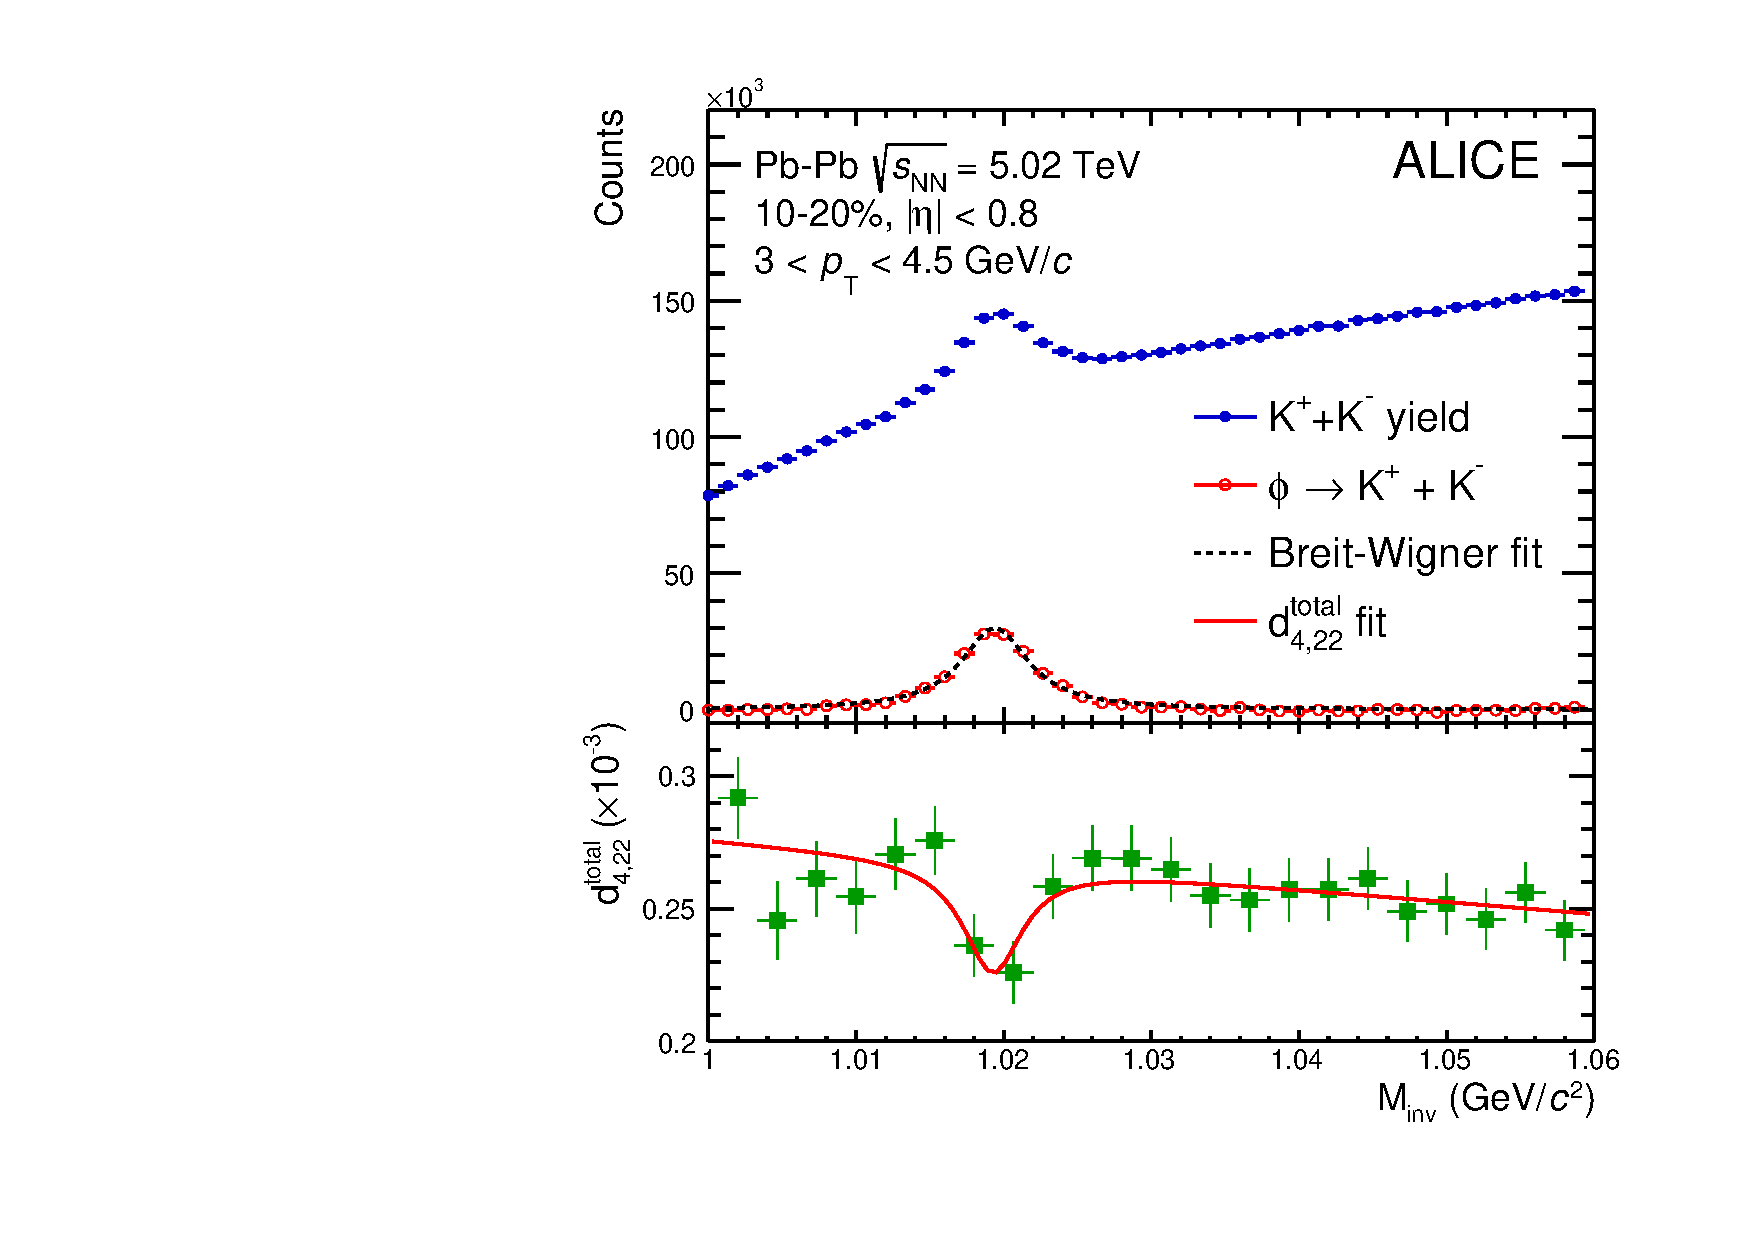
\includegraphics[scale=0.45]{figures/analysisMethod/flowmass_Phi.pdf}
\end{center}
\caption{Reconstruction and $d_{4,22}$ measurement of $\phi$-meson. Upper panel: extraction of $N^{\rm{sig}}$ and $N^{\rm{bkg}}$ by fitting the invariant mass ($m_{\rm{inv}}$) distribution for $\phi$-meson for $3<p_{\rm{T}}<4.5~{\rm GeV}/c$ at 10-20\% centrality interval, lower panel: extraction of $d_{4,22}^{sig}$ by fitting Eq. \ref{Eq:dnmk} to the invariant mass dependence of $d_{4,22}$}
\label{d422_phi_meson}
\end{figure}


%To estimate the signal and background yields, the invariant mass distributions of selected candidates are fitted with sum of the signal and background yields. 
\section{Systematic uncertainties}
\label{Sec:Systematics}
%The systematic uncertainties are estimated by varying the selection criteria for all particle species as well as topological reconstruction requirements for \Ks, \lambdas~and $\phi$.

The systematic uncertainties are estimated by varying the selection criteria for all particle species as well as topological reconstruction requirements for \Ks, \lambdas~and $\phi$. The contributions from different sources are extracted from the relative ratio of the \pT-differential $v_{n,mk}$ between the default selection criteria described in Section~\ref{Sec:EventTrackIdentification} and their variations summarised in Tabs.~\ref{SysVar} and \ref{tab:V0scuts}. Each source with a statistically significant contribution, i.e. $|x_1 - x_2| / \sqrt(|\sigma_{1}^{2} \pm \sigma_{2}^{2}|)  > 1$ (known as barlow check \DIFaddbegin \DIFadd{\mbox{%DIFAUXCMD
\cite{Barlow:2002yb}}%DIFAUXCMD
}\DIFaddend ) was fitted to create a smooth change along \pT~and then the value of these fits were added in quadrature to form the final value of the systematic uncertainties on the non-linear flow modes. An overview of the magnitude of the relative systematic uncertainties per particle species is given in Tab. \ref{SystematicsValues:PID} for \pion, \kaon~and \proton~and Tab. \ref{SystematicsValues:V0} for \Ks, \lambdas~and $\phi$-meson. Systematic uncertainties are grouped into five categories, i.e. event selection, tracking, particle identification, topological cuts and non-flow contribution and are described below.


\begin{table}
\centering
 \DIFdelbeginFL %DIFDELCMD < \resizebox{0.75\textwidth}{!}{\begin{tabular}[!b]{|l|c|c|}
%DIFDELCMD < \hline
%DIFDELCMD < Selection requirement & Default cut & Variations\\
%DIFDELCMD < \hline
%DIFDELCMD < \hline
%DIFDELCMD < Primary $vtx_{z}$ & $\pm$10cm & $\pm$6cm, $\pm$8cm\\ 
%DIFDELCMD < Centrality estimator  & V0M & CL0, CL1\\ 
%DIFDELCMD < Magnetic field polarity & both fields & ++, - - \\
%DIFDELCMD < pile-up rejection & strict & loose \\ \hline
%DIFDELCMD < Tracking mode & global (96) & hybrid (768)\\
%DIFDELCMD < Number of \TPC~space-points &70& 80, 90, 100\\
%DIFDELCMD < $\chi^2$ per \TPC~space-point & 4 & 2 \\
%DIFDELCMD < $\rm{DCA}_{xy}$ cm&$p_{\rm{T}}$ dependant& 0.2, 0.15~cm\\
%DIFDELCMD < $\rm{DCA}_{z}$ cm&2~cm& 0.2, 0.3~cm\\\hline
%DIFDELCMD < PID method & \pT-dependent &  tight \pT-dependent, Bayesian prob. >80\% \\ \hline
%DIFDELCMD < POI vs. RFP charges & All & ++, - - \\
%DIFDELCMD < $\eta$ gap & 0.0 & 0.4 \\ 
%DIFDELCMD < \hline
%DIFDELCMD < \end{tabular}}
%DIFDELCMD < %%%
\DIFdelendFL \DIFaddbeginFL \resizebox{0.75\textwidth}{!}{\begin{tabular}[!b]{|l|c|c|}
\hline
Selection requirement & Default & Variations\\
\hline
\hline
Primary $vtx_{z}$ & $\pm$10cm & $\pm$6cm, $\pm$8cm\\ 
Centrality estimator  & V0M & CL0, CL1\\ 
Magnetic field polarity & both fields & ++, - - \\
pile-up rejection & strict & loose \\ \hline
Tracking mode & global (96) & hybrid (768)\\
Number of \TPC~space-points &70& 80, 90, 100\\
$\chi^2$ per \TPC~space-point & 4 & 2 \\
$\rm{DCA}_{xy}$ cm&$p_{\rm{T}}$ dependant& 0.2, 0.15~cm\\
$\rm{DCA}_{z}$ cm&2~cm& 0.2, 0.3~cm\\\hline
PID method & \pT-dependent &  tight \pT-dependent, Bayesian prob. >80\% \\ \hline
POI vs. RFP charges & All & ++, - - \\
$\eta$ gap & 0.0 & 0.4 \\ 
\hline
\end{tabular}}
\DIFaddendFL \caption{List of the selection criteria and the corresponding variations used for the estimation of the systematic uncertainties of \pion, \kaon~and \proton}\label{SysVar}
\end{table}

\begin{table}
  \centering
  \DIFdelbeginFL %DIFDELCMD < \resizebox{0.75\textwidth}{!}{\begin{tabular}[!b]{|l|c|c|}
%DIFDELCMD <   \hline
%DIFDELCMD <   Selection requirements & Default cut & Variations\\
%DIFDELCMD <   \hline
%DIFDELCMD <   \hline
%DIFDELCMD <   Reconstruction method (\vo~finder) & offline & online \\
%DIFDELCMD <   TPC refit for both daughters & {\tt AliAODTrack::kTPCrefit} & --\\
%DIFDELCMD <   Kink vertex rejection & {\tt not AliAODVertex::kKink} & --\\
%DIFDELCMD <   Decay vertex (radial position) & 5 < r < 100 cm & 10 < r < 100 cm \\
%DIFDELCMD <   Cosine of pointing angle & > 0.998 & > 0.99 \\
%DIFDELCMD <   Number of crossed TPC clusters & > 70 & > 90 \\
%DIFDELCMD <   Number of TPC clusters used for PID & > 70 & > 90 \\
%DIFDELCMD <   Number of findable TPC clusters & > 1 & -- \\
%DIFDELCMD <   Ratio of crossed to findable TPC clusters & > 0.8 & > 1.0\\
%DIFDELCMD <   DCA decay products to primary vertex & > 0.1 cm  & > 0.3 cm\\
%DIFDELCMD <   DCA among daughters & < 0.5 cm & < 0.3 cm\\
%DIFDELCMD <   Daughter \pT~acceptance & -- & > 0.2 \GeV\\
%DIFDELCMD <   TPC PID on daugthers &  < 3$\sigma$ & -- \\
%DIFDELCMD <   %Lifetime & < 20 cm \\
%DIFDELCMD <   Armenteros-Podolanski (\Ks) & $q > 0.2 |\alpha|$ & --\\
%DIFDELCMD <   Daughter $\eta$ acceptance & $|\eta|$ < 0.8 & --\\
%DIFDELCMD <   Mother $\eta$ acceptance & $|\eta|$ < 0.8 & --\\
%DIFDELCMD <   Competing inv. mass rejection (\Ks) & < 5~\MeV$^2$ & --\\
%DIFDELCMD <   Competing inv. mass rejection (\lambdas) & < 10~\MeV$^2$ & --\\
%DIFDELCMD <   \hline 
%DIFDELCMD <   \end{tabular}}
%DIFDELCMD <  %%%
\DIFdelendFL \DIFaddbeginFL \resizebox{0.75\textwidth}{!}{\begin{tabular}[!b]{|l|c|c|}
  \hline
  Selection requirements & Default & Variations\\
  \hline
  \hline
  Reconstruction method (\vo~finder) & offline & online \\
  %TPC refit for both daughters & {\tt AliAODTrack::kTPCrefit} & --\\
  %Kink vertex rejection & {\tt not AliAODVertex::kKink} & --\\
  Decay vertex (radial position) & 5 < r < 100 cm & 10 < r < 100 cm \\
  Cosine of pointing angle & > 0.998 & > 0.99 \\
  Number of crossed TPC clusters & > 70 & > 90 \\
  Number of TPC clusters used for PID & > 70 & > 90 \\
  Number of findable TPC clusters & > 1 & -- \\
  Ratio of crossed to findable TPC clusters & > 0.8 & > 1.0\\
  DCA decay products to primary vertex & > 0.1 cm  & > 0.3 cm\\
  DCA among daughters & < 0.5 cm & < 0.3 cm\\
  Daughter \pT~acceptance & -- & > 0.2 \GeV\\
  TPC PID on daugthers &  < 3$\sigma$ & -- \\
  %Lifetime & < 20 cm \\
  Armenteros-Podolanski (\Ks) & $q > 0.2 |\alpha|$ & --\\
  Daughter $\eta$ acceptance & $|\eta|$ < 0.8 & --\\
  Mother $\eta$ acceptance & $|\eta|$ < 0.8 & --\\
  Competing inv. mass rejection (\Ks) & < 5~\MeV$^2$ & --\\
  Competing inv. mass rejection (\lambdas) & < 10~\MeV$^2$ & --\\
  \hline 
  \end{tabular}}
 \DIFaddendFL \caption{List of topological reconstruction requirements and cuts applied on \vo~candidates including variations for systematical uncertainty study where applicable.} \label{tab:V0scuts}
\end{table}

\DIFdelbegin \DIFdel{Effect of }%DIFDELCMD < {\it %%%
\DIFdel{event selection }%DIFDELCMD < } %%%
\DIFdelend \DIFaddbegin \DIFadd{The effects of event selection }\DIFaddend criteria on the measurements are studied by:  (i) varying \DIFaddbegin \DIFadd{the }\DIFaddend primary vertex position along the beam axis ($z_{vtx}$) from a nominal $\pm$10 cm to $\pm$8 cm and $\pm$6 cm; (ii) changing \DIFaddbegin \DIFadd{the }\DIFaddend centrality estimator from the signal amplitudes in the \DIFdelbegin %DIFDELCMD < \vo %%%
\DIFdelend \DIFaddbegin \DIFadd{V0 }\DIFaddend scintillator detectors to the multiplicity of TPC tracks or the number of SPD clusters; (iii) analysing events recorded for different magnetic field polarities independently; (iv) not rejecting events with tracks caused by pileup. 


\DIFdelbegin \DIFdel{Effect of }%DIFDELCMD < {\it %%%
\DIFdel{tracking}%DIFDELCMD < } %%%
\DIFdel{cuts are then studies by }\DIFdelend \DIFaddbegin \DIFadd{Systematic uncertainties induced by the selection criteria imposed at the track level were investigated by}\DIFaddend : (i) changing the tracking from global \DIFaddbegin \DIFadd{mode where combined track information from both TPC and ITS detectors are used }\DIFaddend to hybrid mode \DIFaddbegin \DIFadd{in which track parameters from TPC are used if the algorithm is unable to match the track reconstructed in the TPC with associated ITS clusters}\DIFaddend ; (ii) increasing the number of TPC space points from 70 up to 100 and (iii) \DIFdelbegin \DIFdel{the }\DIFdelend \DIFaddbegin \DIFadd{decreasing the value of the }\DIFaddend $\chi^{2}$ per TPC space point per degree of freedom from 4 to 2; (iv) varying the selection criteria on both the longitudinal and transverse components of the DCA to estimate the impact of secondary particles from a \DIFdelbegin \DIFdel{strick }\DIFdelend \DIFaddbegin \DIFadd{strict }\DIFaddend \pT-dependent cut to 0.15 cm and 2 cm to 0.2 cm, respectively.

%DIF > requiring the third layer of the ITS to be part of the track reconstruction rather than the first two layers only; (ii) using only tracks that have at least three hits per track in theI TS, complemented by tracks without hits in the first two layers of the ITS (in which case the primary interaction vertex is used as an additional constraint for the momentum determination);
\DIFaddbegin 


\DIFaddend Systematic uncertainties associated with the \DIFdelbegin %DIFDELCMD < {\it %%%
\DIFdel{particle identification }%DIFDELCMD < } %%%
\DIFdelend \DIFaddbegin \DIFadd{particle identification }\DIFaddend procedure were studied by varying the PID method from a \pT-dependent \DIFdelbegin \DIFdel{method described in \ref{SubSec:Identification} }\DIFdelend \DIFaddbegin \DIFadd{one described in \ref{SubSec:Track} }\DIFaddend to a stricter version where the purity increases to 95\% (\pion), 80\% (\kaon) and 80\% (\proton) across the entire \pT~range of study. The second \DIFdelbegin \DIFdel{method used is }\DIFdelend \DIFaddbegin \DIFadd{approach used relied on the }\DIFaddend Bayesian method with a probability of at least 80\% which gives an increase in purity to 97\% (\pion), 87\% (\kaon) and 90\% (\proton) across the entire \pT~range of study. 

\DIFdelbegin \DIFdel{The }%DIFDELCMD < {\it %%%
\DIFdelend \DIFaddbegin \DIFadd{In addition, the }\DIFaddend non-flow contribution \DIFdelbegin %DIFDELCMD < } %%%
\DIFdelend is studied by (i) selecting like sign pairs of particles of interest and reference particles to decrease the effect from decay of resonance particles; (ii) applying pseudorapidity gaps between the two subevents from $|\Delta\eta|>0.0$ to $|\Delta\eta|>0.4$.

The \DIFdelbegin %DIFDELCMD < {\it %%%
\DIFdel{topological cuts }%DIFDELCMD < } %%%
\DIFdelend \DIFaddbegin \DIFadd{topological cuts }\DIFaddend were also varied to account for \DIFaddbegin \DIFadd{the }\DIFaddend \vo~and $\phi$-meson reconstruction. The default \vo~finding method is described in Sec. \DIFdelbegin \DIFdel{\ref{SubSec:K0sLambdaRec}}\DIFdelend \DIFaddbegin \DIFadd{\ref{SubSec:K0sLambdaPhiRec}}\DIFaddend . These selection criteria are varied by (i) changing the reconstruction method for \vo~particles from offline to online\DIFdelbegin \DIFdel{method}\DIFdelend ; (ii) varying the minimum radial distance to the primary vertex at which the \vo~can be produced from 5 cm to 10 cm; (iii) changing the minimum value of cosine of pointing angle from 0.998 to 0.99; (iv) varying the minimum number of TPC space points crossed by the \vo~daughter tracks from 70 to 90; (v) changing the requirement on the minimum number of TPC space points that are used in the reconstruction of the \vo~daughter tracks form 70 to 90; (vi) requesting a minimum ratio of crossed to findable TPC clusters from 0.8 to 1.0; (vii) changing the minimum DCA of the \vo~daughter tracks to the primary vertex from 0.1 cm to 0.3 cm; (viii) changing the maximum DCA of the \vo~daughter tracks to the secondary vertex from 0.5 cm to 0.3 cm; (ix) requiring a minimum \pT~of the \vo~daughter tracks of 0.2 \GeV. 
\DIFdelbegin %DIFDELCMD < \\
%DIFDELCMD < %%%
\DIFdelend 

\DIFaddbegin \DIFadd{The contributions from each source were added in quadrature to form the total systematic uncertainties. This will be represented in all plots of this article as a box around each data point while the statistical uncertainty will be shown by the error bars.
}

\DIFaddend %Tables \ref{SystematicsValues:v422}, \ref{SystematicsValues:v532}, \ref{SystematicsValues:v633} and \ref{SystematicsValues:v6222} summarise the maximum deviations for each individual systematic source over all transverse momenta and centrality intervals in five aforementioned categories. %Selection criteria are grouped into different categories, i.e. event selection, tracking, particle identification, topological cuts and non-flow contribution.


%This change resulted in a minimum and maximum contribution of 0-2\% (\pion), 1-3\% (\kaon), 0-3\% (proton), 0\% (\Ks), 0-2\% (\lambdas) and 1\% ($\phi$-meson) for $v_{4,22}$ across the entire transverse momenta of interest and centrality intervals. Similar effect is observed for $v_{5,32}$ with a minimum and maximum contribution of 0-3\% (\pion), 1-3\% (\kaon), 1-4\% (proton), 0\% (\Ks) and 0-3\% (\lambdas). The variations resulted in larger systematic uncertainties for the sixth order non-linear modes with a minimum and maximum contribution of 3-5\% (\pion), 2-5\% (\kaon), 3-5\% (proton), 0\% (\Ks) and 1-3\% (\lambdas) for $v_{6,33}$ and 2-7\% (\pion), 2-7\% (\kaon) and 4-7\% (proton) for $v_{6,222}$.

\begin{table}[!ht]
\resizebox{\textwidth}{!}{\begin{tabular}{ |p{4.5cm} |l|c|c|c|c|c|c|c|c|c|c|c|c|}
\hline
\multicolumn{1}{| c |}{} & \multicolumn{3}{| c |}{ $v_{4,22}$ } & \multicolumn{3}{| c |}{ $v_{5,32}$} & \multicolumn{3}{| c |}{ $v_{6,33}$} & \multicolumn{3}{| c |}{ $v_{6,222}$} \\
\hline
Error source  & \pion &  \kaon & \proton &  \pion & \kaon & \proton &  \pion &  \kaon & \proton &  \pion &  \kaon & \proton \\ \hline  \hline
Primary $z_{vtx}$  & 0-2\% & 1-3\% & 0-3\% & 0-3\% & 1-3\% & 1-4\% & 3-5\% & 2-5\% & 3-5\% & 2-7\% & 2-7\% & 4-7\%\\
Centrality estimator  & 0-4\% & 1-4\% & 1-5\% & 0-4\% & 1-3\% & 2-4\% & 4-10\% & 4-10\% & 5-10\% & 3-10\% & 5-10\% & 4-10\%\\
Magnetic field polarity & 0-2\% & 0-3\% & 0-3\% & 0-4\% & 0-5\% & 0-5\% & 0-10\% & 0-10\% & 0-10\% & 0-10\% & 0-10\% & 0-10\% \\
Pileup rejection & 0-4\% & 0-4\% & 0-4\% & 0-5\% & 1-5\% & 0-5\% & 5-7\% & 5-10\% & 5-8\% & 4-10\% & 4-10\% & 2-10\%\\\hline
Tracking mode  & 1-4\% & 1-5\% & 1-4\% & 2-6\% & 3-5\% & 2-8\% & 0-8\% & 0-7\% & 3-8\% & 1-10\% & 4-10\% & 2-10\% \\
Number of \TPC~space-points &  1-2\% & 0-2\% & 0-2\% & 0-3\% & 1-3\% & 1-3\% & 4-8\% & 3-8\% & 3-8\% & 2-8\% & 4-8\% & 4-8\% \\
$\chi^2$ per \TPC~space-point & 0-2\% & 1-2\% & 1-3\% & 1-3\% & 1-3\% & 2-4\% & 3-5\% & 3-6\% & 3-6\% & 2-6\% & 4-7\% & 4-7\%\\
DCAxy & 0-2\% & 0-2\% & 1-3\% & 0-3\% & 1-3\% & 1-3\% & 2-7\% & 2-8\% & 4-8\% & 2-8\% & 4-8\% & 3-8\%\\
DCAz & 0-3\% & 0-2\% & 1-2\% & 1-2\% & 1-3\% & 2-3\% & 3-7\% & 3-7\% & 5-7\% & 2-7\% & 4-8\% & 2-8\%\\\hline
Particle identification & 1-5\% & 1-5\% & 1-3\% & 1-5\% & 2-5\% & 1-5\% & 5-10\% & 5-10\% & 6-12\% & 4-12\% & 6-15\% & 4-15\%\\\hline
POI vs. RFP charges & 0-2\% & 0-3\% & 2-3\% & 0-4\% & 0-4\% & 2-4\% & 0-4\% & 0-6\% & 0-6\% & 0\% & 0\% & 0\% \\ 
$\eta$ gap & 1-3\% & 1-4\% & 1-2\% & 1-4\% & 1-4\% & 1-5\% & 0-5\% & 0-5\% & 0-5\% & 0\% & 0\% & 0\%  \\\hline 
%\hline
\end{tabular}}
\caption{List of the maximum systematic uncertainties from each individual source for $v_{n,mk}$ of \pion, \kaon~and \proton. The uncertainties depend on the transverse momenta and centrality interval. Hence here maximum and minimum values are listed.}\label{SystematicsValues:PID}
\end{table}

\begin{table}[!ht]
\centering
\resizebox{0.75\textwidth}{!}{\begin{tabular}{ |p{6.7cm} |l|c|c|c|c|c|c|c|}
\hline
\multicolumn{1}{| c |}{} & \multicolumn{3}{| c |}{ $v_{4,22}$ } & \multicolumn{2}{| c |}{ $v_{5,32}$} & \multicolumn{2}{| c |}{ $v_{6,33}$} \\
\hline
Error source  & \Ks &  \lambdas & $\phi$ &  \Ks &  \lambdas & \Ks &  \lambdas   \\ \hline  \hline
Primary $z_{vtx}$  & 0\% & 0-2\% & 1\% & 0\% & 0-3\% & 0\% & 1-3\%\\ \hline
Tracking mode  & - & - & 2\% & - & - & - & - \\
Number of \TPC~space-points & 0-3\% & 1-2\% & 2\% & 0\% & 2\% & 0\% & 2\%  \\ \hline
Particle identification & - & - & 4-6\% & - & - & - & -\\\hline
Reconstruction method (\vo~finder) & 3-5\% & 2-3\% & N/A & 5\% & 1\% & 5\% & 1\%   \\
Decay radius & 3-5\% & 1-3\% & N/A & 5-6\% & 0-2\% & 5\% & 2\%\\
Ratio of crossed to findable TPC clusters & 0-2\% & 0-3\% & N/A & 0\%  & 1-2\% & 0\% & 3\%  \\
DCA decay products to primary vertex & 2-5\% & 2-4\% & N/A & 4-5\% & 2-3\% & 5\% & 2-3\%  \\
DCA between decay products & 0-3\% & 1-2\% & N/A & 0-4\% & 0-4\% & 0\% & 0-4\% \\
Pointing angle $\cos(\theta_{\rm p})$ & 3-4\% & 0-2\% & N/A & 3-4\% & 0-3\% & 3\% & 1\%  \\
Minimum \pT~of daughter tracks & 1-3\% & 0-1\% & N/A & 2-3\% & 2-3\% & 0\% & 0-3\%  \\ \hline
%$\eta$ gap & - & - & - & - & - & - & -  \\\hline 
%\hline
\end{tabular}}
\caption{List of the maximum systematic uncertainties from each individual source for $v_{n,mk}$ of \Ks, \lambdas~and $\phi$-meson. The uncertainties depend on the transverse momenta and centrality interval. Hence here maximum and minimum values are listed. "N/A" indicates that a certain check was not applicable to the given particle of interest. If a source was checked and proved to be of negligible effect, the field is marked with "-".}\label{SystematicsValues:V0}
\end{table}


%\begin{table}[!htb]
%\centering
%\begin{tabular}{ |p{7cm} |l|c|c|c|c|c|}
%\hline
%Error source  & \pion &  \kaon & \proton &  \Ks & \lambdas & $\phi$ \\ \hline  \hline
%Primary $z_{vtx}$  & 0-2\% & 1-3\% & 0-3\% & 0\% & 0-2\% & 1\%  \\
%Centrality estimator  & 0-4\% & 1-4\% & 1-5\% & - & - & -  \\
%Magnetic field polarity & 0-2\% & 0-3\% & 0-3\% & - & - & -  \\
%Pileup rejection & 0-4\% & 0-4\% & 0-4\% & - & - & -  \\\hline
%Tracking mode  & 1-4\% & 1-5\% & 1-4\% & - & - & 2\%  \\
%Number of \TPC~space-points & 1-2\% & 0-2\% & 0-2\% & 0-3\% & 1-2\% & 2\%  \\
%$\chi^2$ per \TPC~space-point & 0-2\% & 1-2\% & 1-3\% & - & - & -  \\
%DCAxy & 0-2\% & 0-2\% & 1-3\% & - & - & -  \\
%DCAz & 0-3\% & 0-2\% & 1-2\% & - & - & -  \\ \hline
%Particle identification & 1-5\% & 1-5\% & 1-3\% & - & - & 4-6\% \\\hline
%Reconstruction method (\vo~finder) & N/A & N/A & N/A & 3-5\% & 2-3\% & N/A  \\
%Decay radius & N/A & N/A & N/A & 3-5\% & 1-3\% & N/A  \\
%Ratio of crossed to findable TPC clusters & N/A & N/A & N/A & 0-2\% & 0-3\% & N/A  \\
%DCA decay products to primary vertex & N/A & N/A & N/A & 2-5\% & 2-4\% & N/A  \\
%DCA between decay products & N/A & N/A & N/A & 0-3\% & 1-2\% & N/A  \\
%Pointing angle $\cos(\theta_{\rm p})$ & N/A & N/A & N/A & 3-4\% & 0-2\% & N/A  \\
%Minimum \pT~of daughter tracks & N/A & N/A & N/A & 1-3\% & 0-1\% & N/A  \\ \hline
%POI vs. RFP charges & 0-2\% & 0-3\% & 2-3\% & - & - & - \\
%$\eta$ gap & 1-3\% & 1-4\% & 1-2\% & - & - & - \\
%\hline 
%\end{tabular}
%\caption{List of the maximum systematic uncertainties from each individual source for $v_{4,22}$ of \pion, \kaon, \proton, \Ks, \lambdas~and $\phi$-meson. The uncertainties depend on the transverse momenta and centrality interval. Hence here maximum and minimum values are listed. "N/A" indicated that a certain check was not applicable to the given particle of interest. If a source was checked and proved to be of negligible effect, the field is marked with "-".}\label{SystematicsValues:v422}
%\end{table}


%\begin{table}[!htb]
%\centering
%\begin{tabular}{ |p{7cm} |l|c|c|c|c|c|}
%\hline
%Error source  & \pion &  \kaon & \proton &  \Ks & \lambdas  \\ \hline  \hline
%Primary $z_{vtx}$  & 0-3\% & 1-3\% & 1-4\% & 0\% & 0-3\%   \\
%Centrality estimator  & 0-4\% & 1-3\% & 2-4\% & - & -   \\
%Magnetic field polarity & 0-4\% & 0-5\% & 0-5\% & - & -    \\
%Pileup rejection & 0-5\% & 1-5\% & 0-5\% & - & - \\\hline
%Tracking mode  & 2-6\% & 3-5\% & 2-8\% & - & -   \\
%Number of \TPC~space-points & 0-3\% & 1-3\% & 1-3\% & 0\% & 2\%   \\
%$\chi^2$ per \TPC~space-point & 1-3\% & 1-3\% & 2-4\% & - & -   \\
%DCAxy & 0-3\% & 1-3\% & 1-3\% & - & -  \\
%DCAz & 1-2\% & 1-3\% & 2-3\% & - & -   \\ \hline
%Particle identification & 1-5\% & 2-5\% & 1-5\% & - & -  \\\hline
%Reconstruction method (\vo~finder) & N/A & N/A & N/A & 5\% & 1\%  \\
%Decay radius & N/A & N/A & N/A & 5-6\% & 0-2\%   \\
%Ratio of crossed to findable TPC clusters & N/A & N/A & N/A & 0\%  & 1-2\%  \\
%DCA decay products to primary vertex & N/A & N/A & N/A & 4-5\% & 2-3\%  \\
%DCA between decay products & N/A & N/A & N/A & 0-4\% & 0-4\%  \\
%Pointing angle $\cos(\theta_{\rm p})$ & N/A & N/A & N/A & 3-4\% & 0-3\%  \\
%Minimum \pT~of daughter tracks & N/A & N/A & N/A & 2-3\% & 2-3\%  \\ \hline
%POI vs. RFP charges & 0-4\% & 0-4\% & 2-4\% & - & -  \\
%$\eta$ gap & 1-4\% & 1-4\% & 1-5\% & - & -  \\
%\hline 
%\end{tabular}
%\caption{List of the maximum systematic uncertainties from each individual source for $v_{5,32}$ of \pion, \kaon, \proton, \Ks~and \lambdas. The uncertainties depend on the transverse momenta and centrality interval. Hence here maximum and minimum values are listed. "N/A" indicated that a certain check was not applicable to the given particle of interest. If a source was checked and proved to be of negligible effect, the field is marked with "-".}\label{SystematicsValues:v532}
%\end{table}

%\begin{table}[!htb]
%\centering
%\begin{tabular}{ |p{7cm} |l|c|c|c|c|c|}
%\hline
%Error source  & \pion &  \kaon & \proton &  \Ks & \lambdas  \\ \hline  \hline
%Primary $z_{vtx}$  & 3-5\% & 2-5\% & 3-5\% & 0\% & 1-3\%   \\
%Centrality estimator  & 4-10\% & 4-10\% & 5-10\% & - & -   \\
%Magnetic field polarity & 0-10\% & 0-10\% & 0-10\% & - & -    \\
%Pileup rejection & 5-7\% & 5-10\% & 5-8\% & - & - \\\hline
%Tracking mode  & 0-8\% & 0-7\% & 3-8\% & - & -   \\
%Number of \TPC~space-points & 4-8\% & 3-8\% & 3-8\% & 0\% & 2\%   \\
%$\chi^2$ per \TPC~space-point & 3-5\% & 3-6\% & 3-6\% & - & -   \\
%DCAxy & 2-7\% & 2-8\% & 4-8\% & - & -  \\
%DCAz & 3-7\% & 3-7\% & 5-7\% & - & -   \\ \hline
%Particle identification & 5-10\% & 5-10\% & 6-12\% & - & -  \\\hline
%Reconstruction method (\vo~finder) & N/A & N/A & N/A & 5\% & 1\%  \\
%Decay radius & N/A & N/A & N/A & 5\% & 2\%   \\
%Ratio of crossed to findable TPC clusters & N/A & N/A & N/A & 0\% & 3\%  \\
%DCA decay products to primary vertex & N/A & N/A & N/A & 5\% & 2-3\%  \\
%DCA between decay products & N/A & N/A & N/A & 0\% & 0-4\%  \\
%Pointing angle $\cos(\theta_{\rm p})$ & N/A & N/A & N/A & 3\% & 1\%  \\
%Minimum \pT~of daughter tracks & N/A & N/A & N/A & 0\% & 0-3\%  \\ \hline
%POI vs. RFP charges & 0-4\% & 0-6\% & 0-6\% & - & -  \\
%$\eta$ gap & 0-5\% & 0-5\% & 0-5\% & - & -  \\
%\hline 
%\end{tabular}
%\caption{List of the maximum systematic uncertainties from each individual source for $v_{6,33}$ of \pion, \kaon, \proton, \Ks~and \lambdas. The uncertainties depend on the transverse momenta and centrality interval. Hence here maximum and minimum values are listed. "N/A" indicated that a certain check was not applicable to the given particle of interest. If a source was checked and proved to be of negligible effect, the field is marked with "-".}\label{SystematicsValues:v633}
%\end{table}


%\begin{table}[!htb]
%\centering
%\begin{tabular}{ |p{6cm} |l|c|c|c|}
%\hline
%Error source  & \pion &  \kaon & \proton  \\ \hline  \hline
%Primary $z_{vtx}$  & 2-7\% & 2-7\% & 4-7\%  \\
%Centrality estimator  & 3-10\% & 5-10\% & 4-10\%  \\
%Magnetic field polarity & 0-10\% & 0-10\% & 0-10\%  \\
%Pileup rejection & 4-10\% & 4-10\% & 2-10\% \\\hline
%Tracking mode  & 1-10\% & 4-10\% & 2-10\%   \\
%Number of \TPC~space-points & 2-8\% & 4-8\% & 4-8\%  \\
%$\chi^2$ per \TPC~space-point & 2-6\% & 4-7\% & 4-7\%   \\
%DCAxy & 2-8\% & 4-8\% & 3-8\%  \\
%DCAz & 2-7\% & 4-8\% & 2-8\%   \\ \hline
%Particle identification & 4-12\% & 6-15\% & 4-15\%  \\\hline
%POI vs. RFP charges & 0\% & 0\% & 0\% \\
%$\eta$ gap & 0\% & 0\% & 0\% \\
%\hline 
%\end{tabular}
%\caption{List of the maximum systematic uncertainties from each individual source for $v_{6,222}$ of \pion, \kaon, \proton, \Ks~and \lambdas. The uncertainties depend on the transverse momenta and centrality interval. Hence here maximum and minimum values are listed. "N/A" indicated that a certain check was not applicable to the given particle of interest. If a source was checked and proved to be of negligible effect, the field is marked with "-".}\label{SystematicsValues:v6222}
%\end{table}


\newpage

\section{Results and discussion}
\label{Sec:Results}

In this section, the results for the \pT-dependent non-linear flow modes $v_{4,22}$, $v_{5,32}$, $v_{6,33}$ and $v_{6,222}$ of identified particles are presented for various centrality intervals in Pb--Pb collisions at \sNN. We first present the centrality and \pT~dependence of $v_{n,mk}$ in Sec. \ref{SubSec:pTdependence}. \DIFdelbegin \DIFdel{Scaling }\DIFdelend \DIFaddbegin \DIFadd{The scaling }\DIFaddend properties of non-linear flow modes are \DIFdelbegin \DIFdel{discussed in Sec. \ref{subsection:NCQscaling} and comparisons }\DIFdelend \DIFaddbegin \DIFadd{also discussed in this section. Comparisons }\DIFaddend to two model calculations are shown in Sec. \ref{SubSec:hydro}. Note that the same data are used in different representations to highlight the physics implications of the measurements in each section. 
%~for 0-5\% up to 50-60\% centrality intervals for \pion, \kaon, \proton, \Ks, \lambdas~and $\phi$-meson

\subsection{Centrality and \pT~dependence of non-linear flow modes}
\label{SubSec:pTdependence}

Higher order flow coefficients ($n>3$) are mainly generated by inhomogeneities in the initial density profile, the collision geometry as well as the non-linear hydrodynamic response of the system. Figure \ref{v422_centralityDependence} presents the non-linear term for the fourth order flow coefficient, i.e. $v_{4,22}(p_{\rm{T}})$, of \pion, \kaon, \proton, \lambdas, \Ks~and $\phi$-meson for a wide range of centrality intervals, i.e. 0-60\%. For the $\phi$-meson, the results are reported in the 10-50\% centrality interval, where $v_{4,22}$ can be measured accurately. The magnitude of $v_{4,22}$ rises steeply with increasing centrality interval from 0-5\% to 40-50\% for all particle species. This increase is expected as $v_{4,22}$ measures the contribution of the second order eccentricity, $\varepsilon_{2}$, in $v_{4}$ \DIFdelbegin \DIFdel{and the eccentricity of
the overlap region of the colliding nuclei }\DIFdelend \DIFaddbegin \DIFadd{which }\DIFaddend increases for peripheral collisions \DIFaddbegin \DIFadd{\mbox{%DIFAUXCMD
\cite{Alver:2010gr}}%DIFAUXCMD
}\DIFaddend . For more peripheral collisions (i.e. 50-60\%) , the magnitude of $v_{4,22}$ is smaller than in the previous centrality intervals for all particle species. This \DIFaddbegin \DIFadd{effect that was observed also in $v_n$ measurements }\DIFaddend is probably due to the shorter lifetime of the produced system in more peripheral collisions, which \DIFdelbegin \DIFdel{stops }\DIFdelend \DIFaddbegin \DIFadd{prevents }\DIFaddend $v_{4,22}$ from developing further. 


\begin{figure}[!htb]
\begin{center}
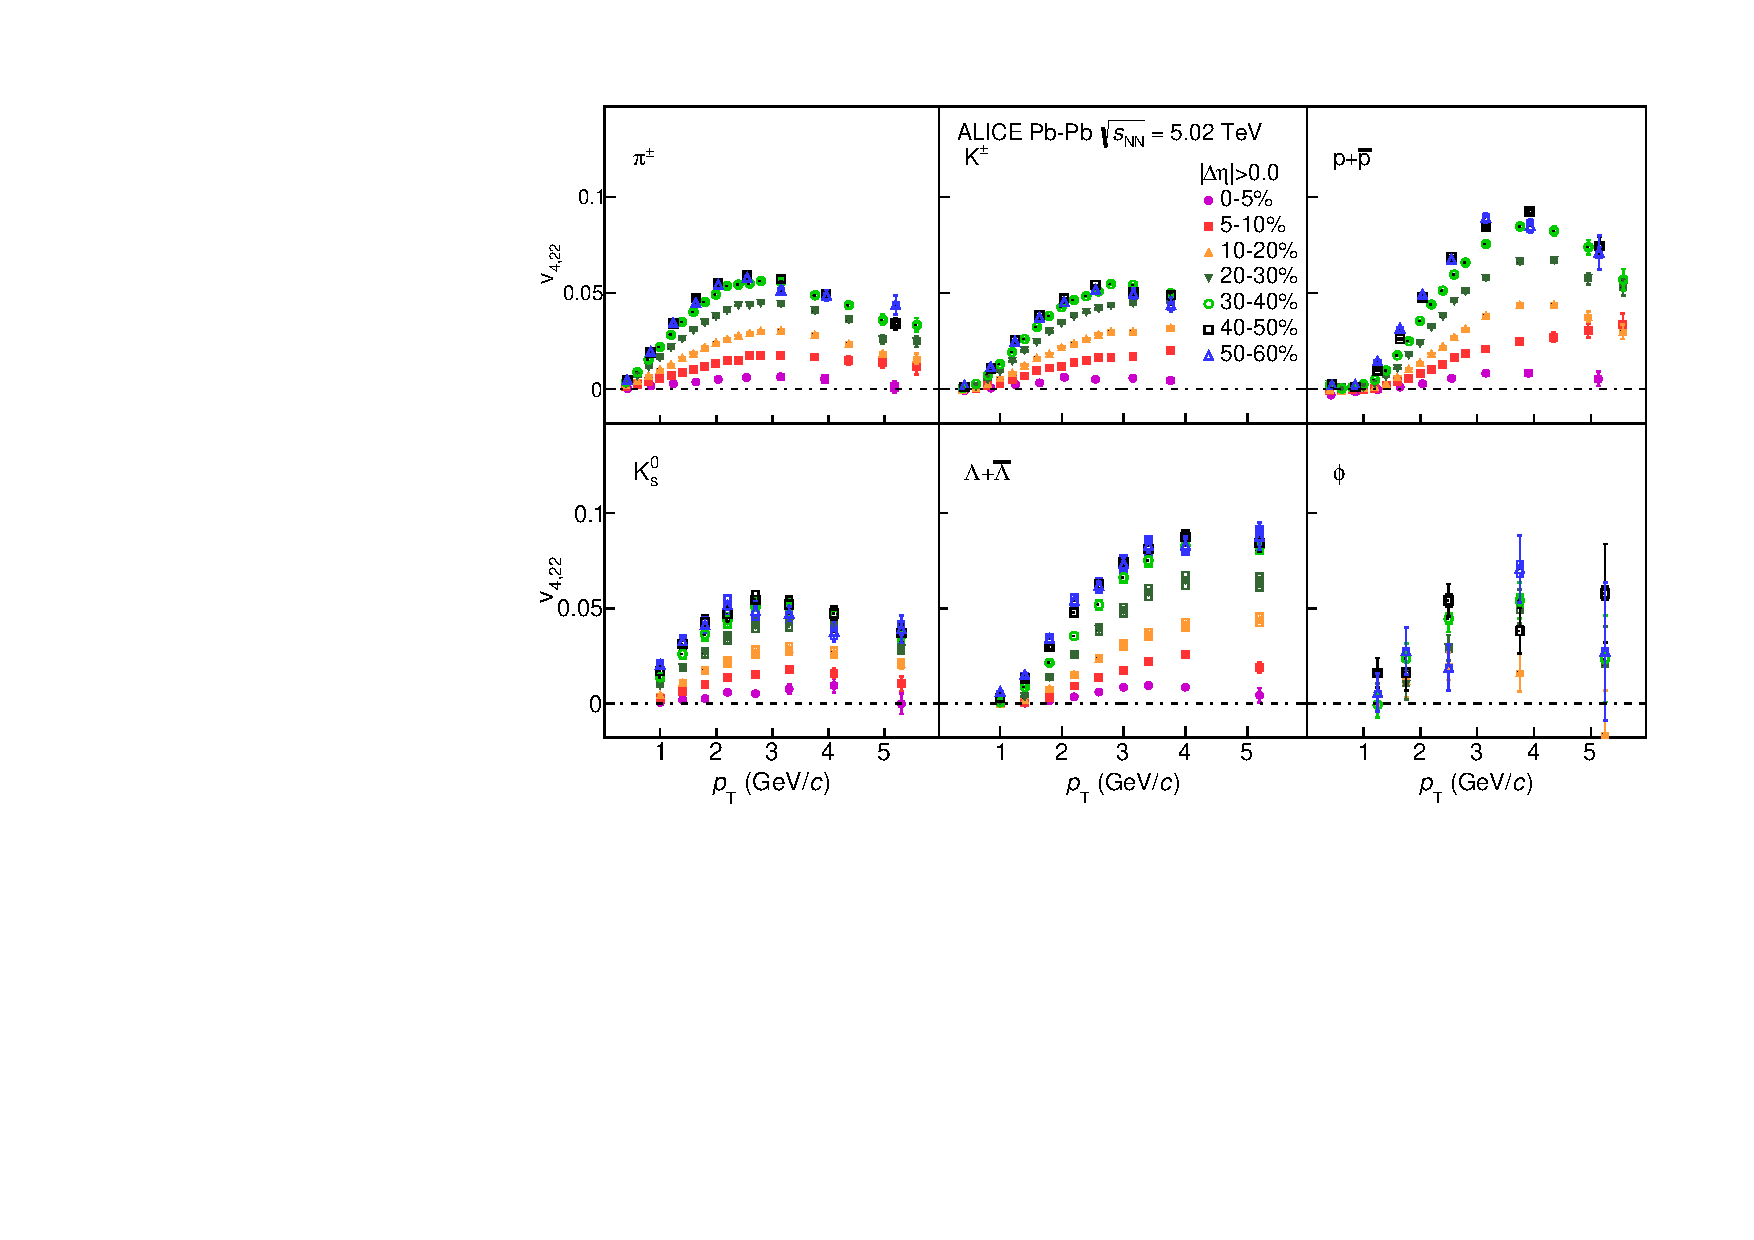
\includegraphics[scale=0.82]{figures/results/All_v422_gap00_CentDep_PID2.pdf}
\end{center}
\caption{The \pT-differential $v_{4,22}$ for different centrality intervals of Pb--Pb collisions at \sNN~ grouped by particle species.}
\label{v422_centralityDependence}
\end{figure}

Figure \ref{v523_centralityDependence} presents the non-linear term for the fifth order flow coefficient, i.e. $v_{5,32}(p_{\rm{T}})$, of \pion, \kaon, \proton, \lambdas~and \Ks~for the same range of centrality intervals, i.e. 0-60\%. Statistical precision limits extending the measurements of non-linear flow modes of $\phi$-meson for $n>4$. The measurements show a significant increase in the magnitude of this non-linear flow mode with increasing centrality percentile. \DIFdelbegin \DIFdel{Similar to $v_{4,22}$, this trend was expected }\DIFdelend \DIFaddbegin \DIFadd{This is }\DIFaddend due to the \DIFdelbegin \DIFdel{contribution of the second order eccentricity, }\DIFdelend \DIFaddbegin \DIFadd{fact that $v_{5,32}(p_{\rm{T}})$ has a contribution from both }\DIFaddend $\varepsilon_{2}$ \DIFaddbegin \DIFadd{and $\varepsilon_{3}$. It is shown in MC studies that both $\varepsilon_{2}$ and $\varepsilon_{3}$ increase for peripheral collisions \mbox{%DIFAUXCMD
\cite{Alver:2010gr}}%DIFAUXCMD
. Although, this increase is less pronounced for $\varepsilon_{3}$}\DIFaddend .

\begin{figure}[!htb]
\begin{center}
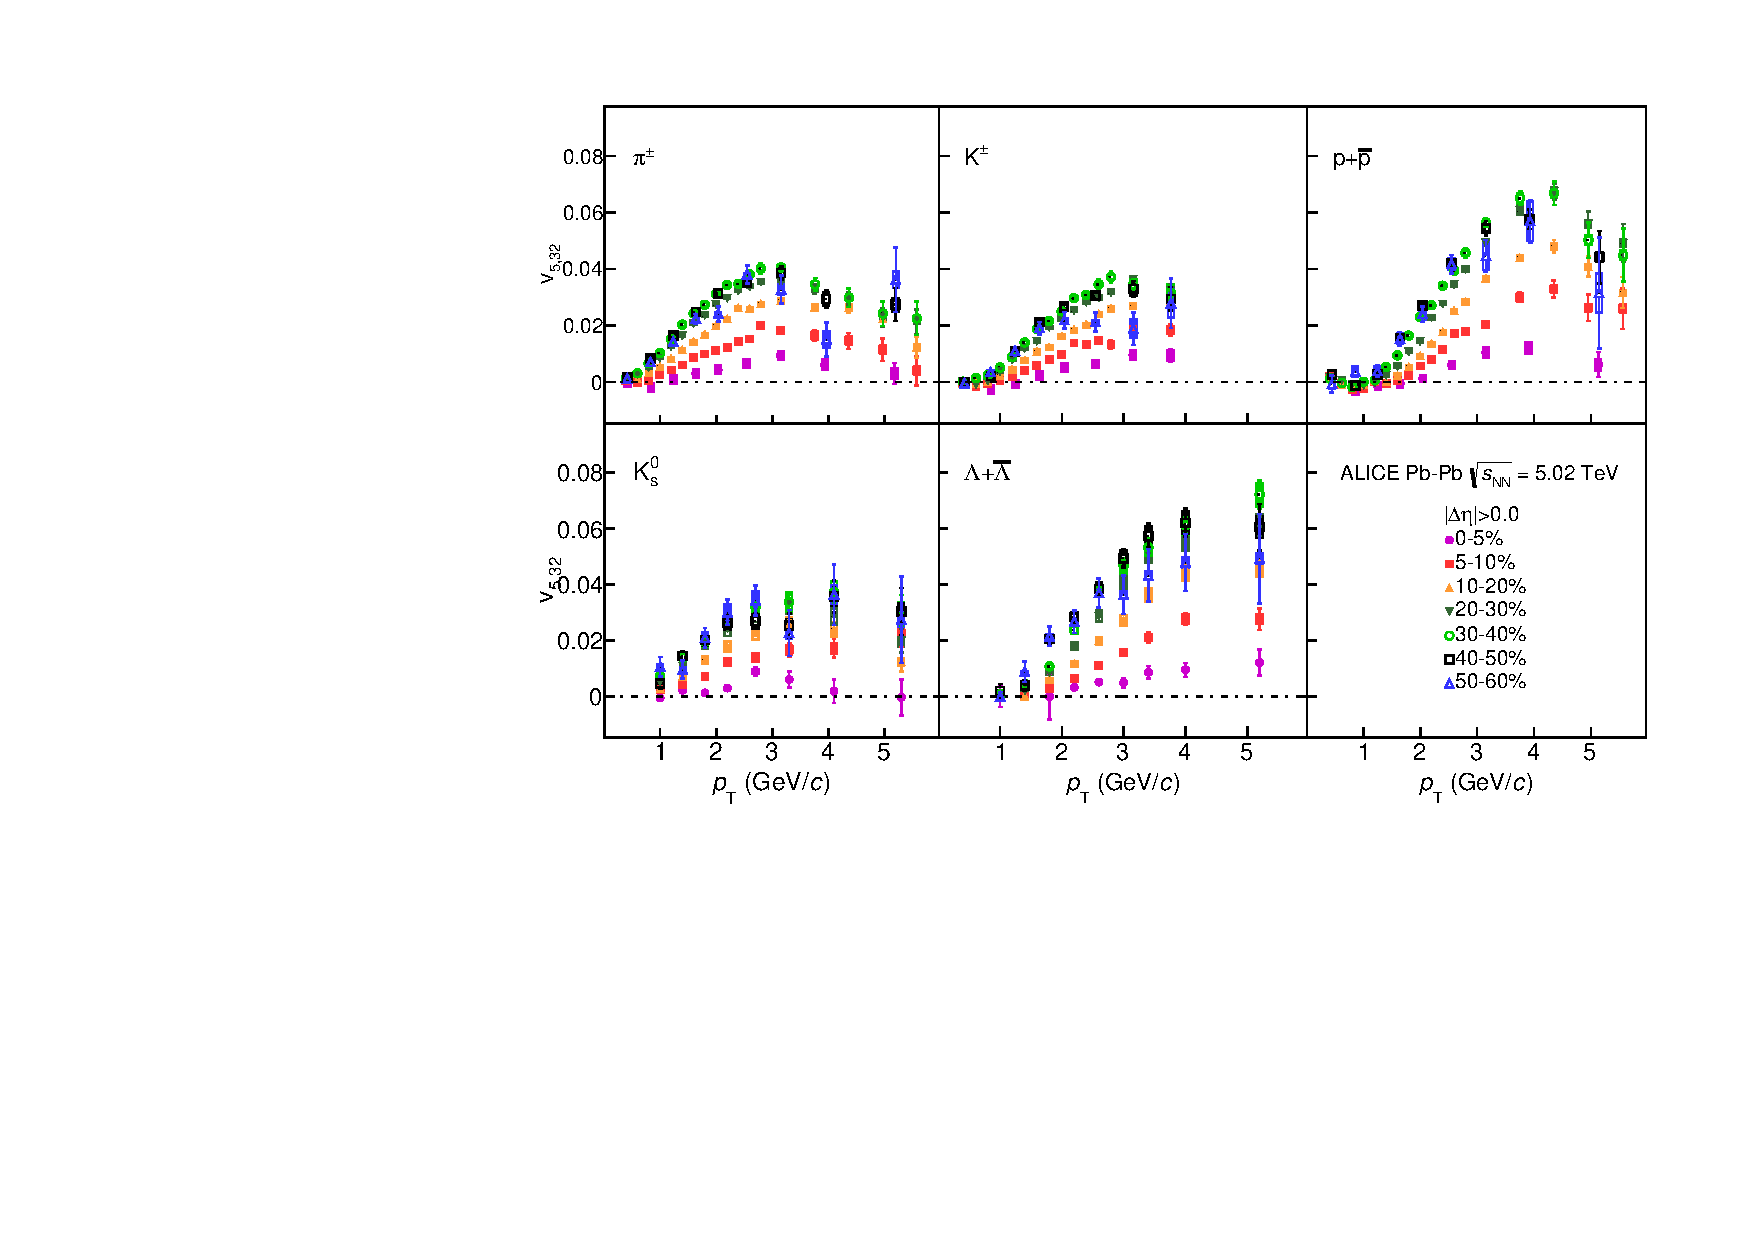
\includegraphics[scale=0.82]{figures/results/All_v523_gap00_CentDep_PID2.pdf}
\end{center}
\caption{The \pT-differential $v_{5,32}$ for different centrality intervals of Pb--Pb collisions at \sNN~ grouped by particle species.}
\label{v523_centralityDependence}
\end{figure}

Figure \ref{v633_centralityDependence} and \ref{v6222_centralityDependence} present the non-linear terms for the sixth order flow coefficient, i.e. $v_{6,33}(p_{\rm{T}})$ for \pion, \kaon, \proton, \lambdas~and \Ks~at 0-50\% centrality intervals and $v_{6,222}(p_{\rm{T}})$ for \pion, \kaon, \proton~at 0-60\% centrality intervals. As expected, measurements of $v_{6,222}(p_{\rm{T}})$ show an increase in the magnitude of this non-linear flow mode with increasing centrality percentile, whereas, $v_{6,33}(p_{\rm{T}})$ presents little to no dependence on centrality. 

\begin{figure}[!htb]
\begin{center}
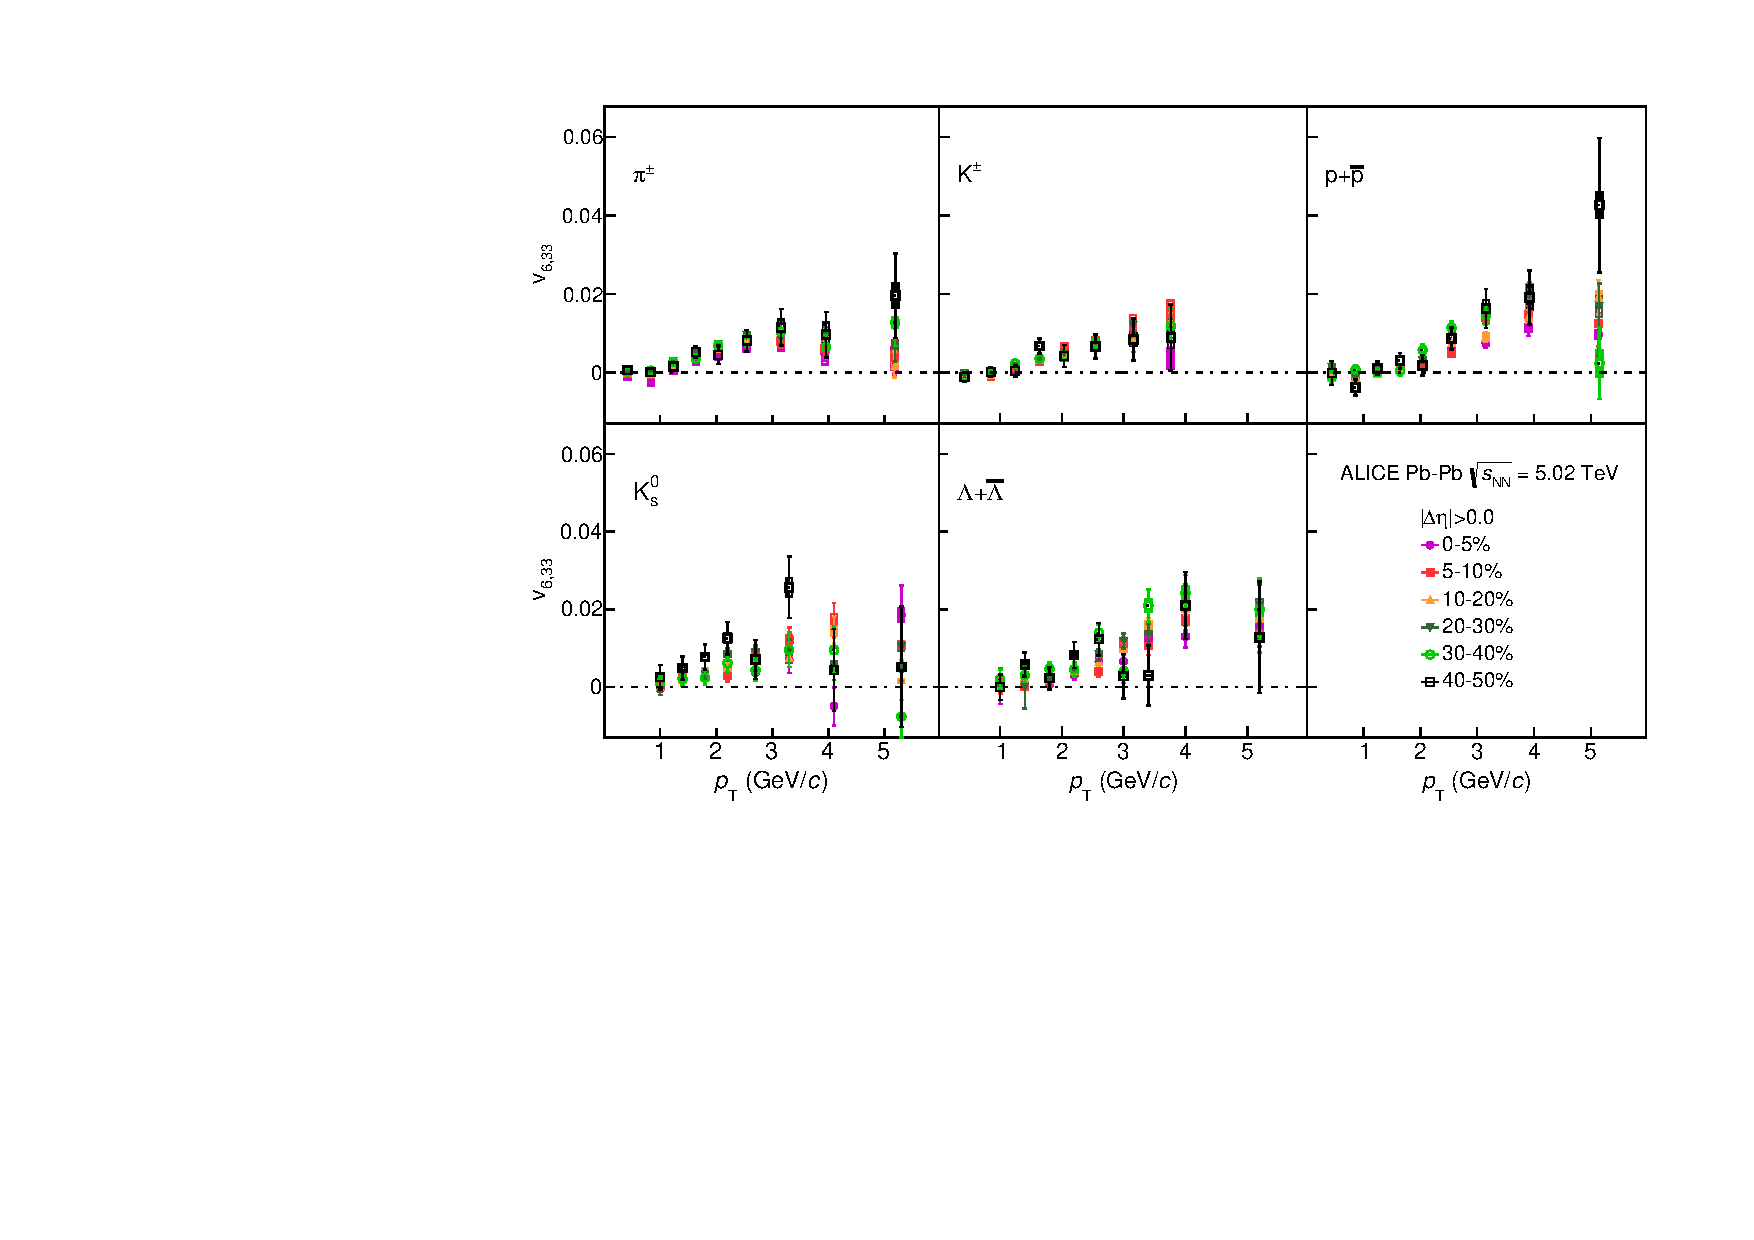
\includegraphics[scale=0.82]{figures/results/All_v633_gap00_CentDep_PID2.pdf}
\end{center}
\caption{The \pT-differential $v_{6,33}$ for different centrality intervals of Pb--Pb collisions at \sNN~ grouped by particle species.}
\label{v633_centralityDependence}
\end{figure}

\begin{figure}[!htb]
\begin{center}
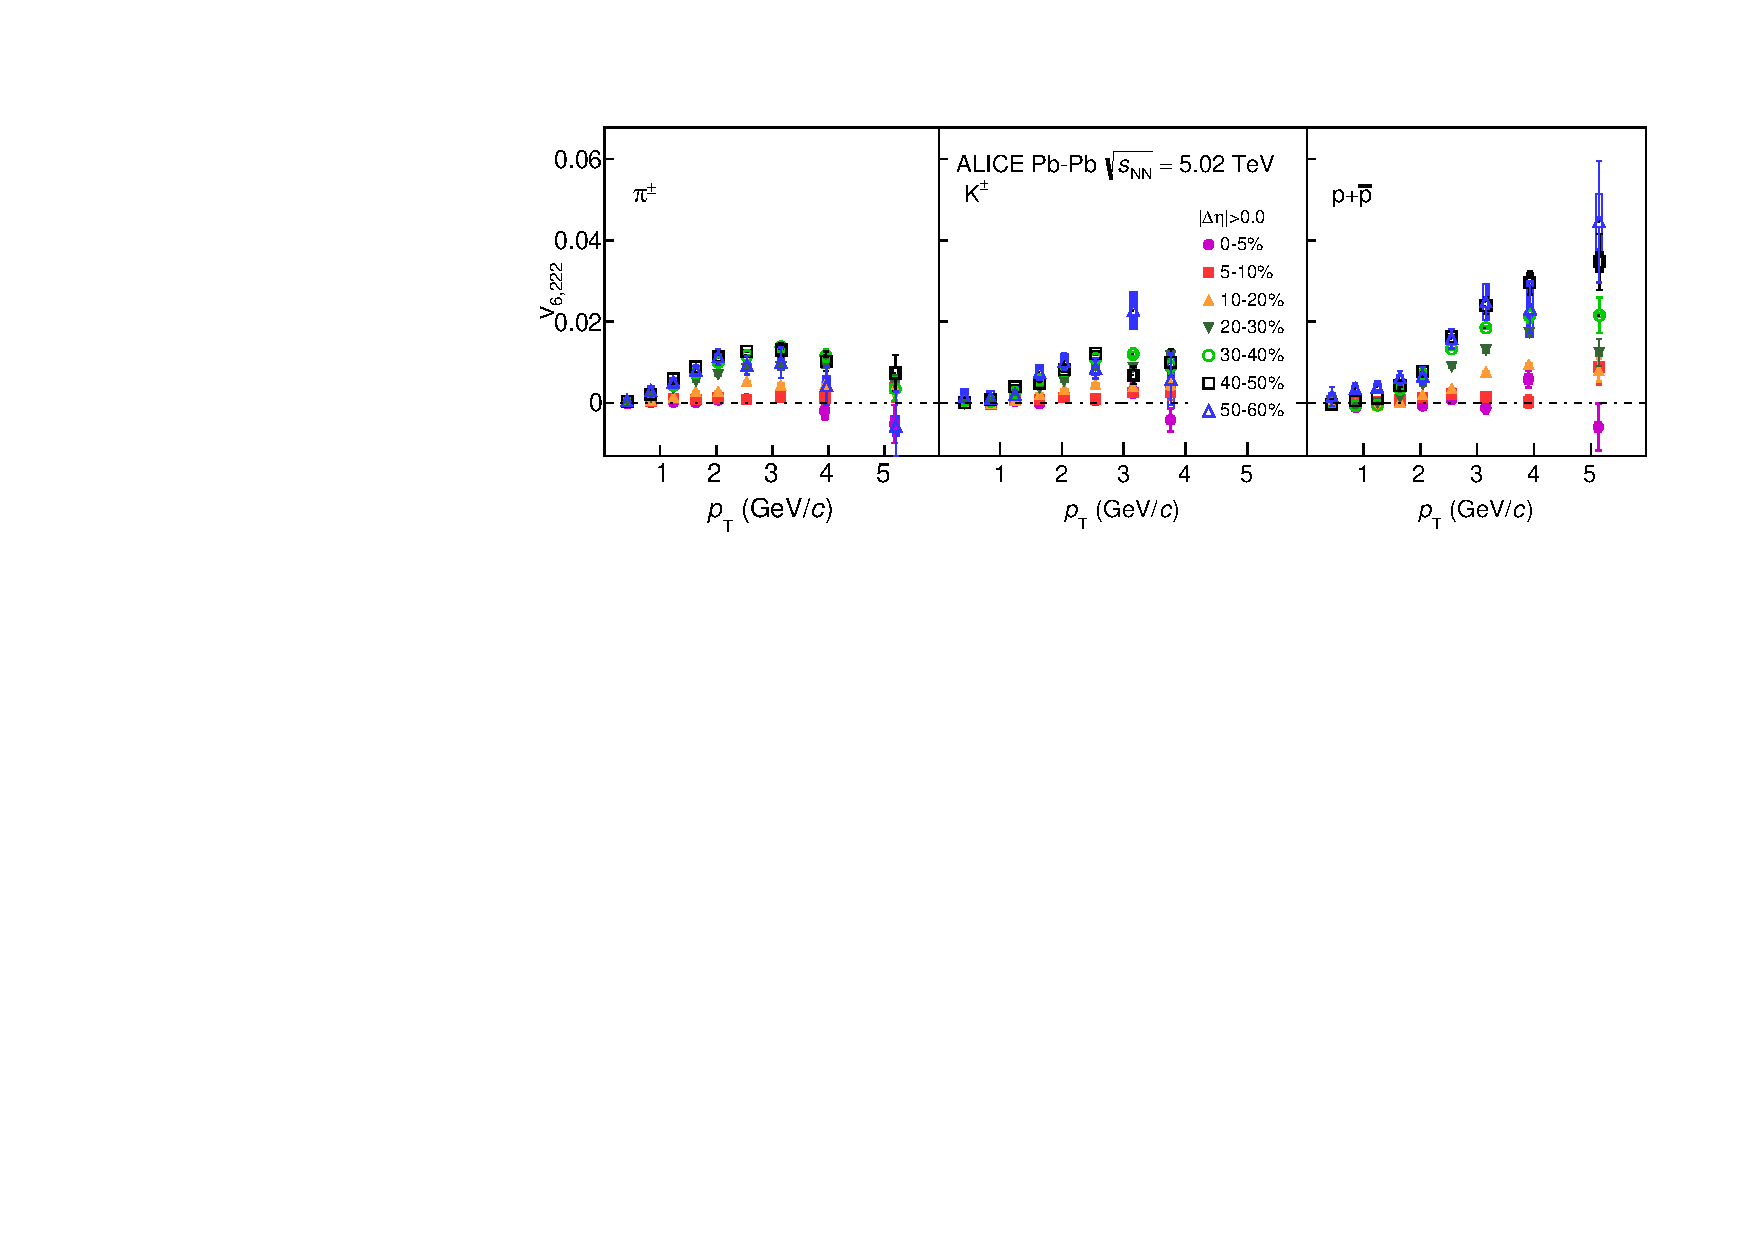
\includegraphics[scale=0.82]{figures/results/All_v6222_gap00_CentDep_PID2.pdf}
\end{center}
\caption{The \pT-differential $v_{6,222}$ for different centrality intervals of Pb--Pb collisions at \sNN~ grouped by particle species.}
\label{v6222_centralityDependence}
\end{figure}

\newpage
%\subsection{Mass ordering}
%\label{MassOrdering}

In Fig. \ref{v422_particleDependence} the same data points are grouped by centrality interval to highlight how $v_{4,22}$ develops for a given centrality for various particle species as a function of \pT.
%Figures \ref{v422_particleDependence} presents the \pT-differential $v_{4,22}$ for \pion, \kaon, \proton, \Ks, \lambdas~and $\phi$-meson starting from most central collisions (0-5\%) up to the 50-60\% centrality interval. 
A clear mass ordering can be seen in the low \pT~region (i.e. \pT $< 2.5$ \GeV) at all collision centralities. This mass dependence arises from the interplay between the \DIFdelbegin \DIFdel{non-linear response of the system }\DIFdelend \DIFaddbegin \DIFadd{anisotropic flow }\DIFaddend and radial flow. Radial flow creates a depletion in the particle spectra at lower \pT~values which leads to lower $v_{4,22}$ for heavier particles \DIFaddbegin \DIFadd{\mbox{%DIFAUXCMD
\cite{Shen:2011eg}}%DIFAUXCMD
}\DIFaddend .


\begin{figure}[!htb]
\begin{center}
\DIFdelbeginFL %DIFDELCMD < 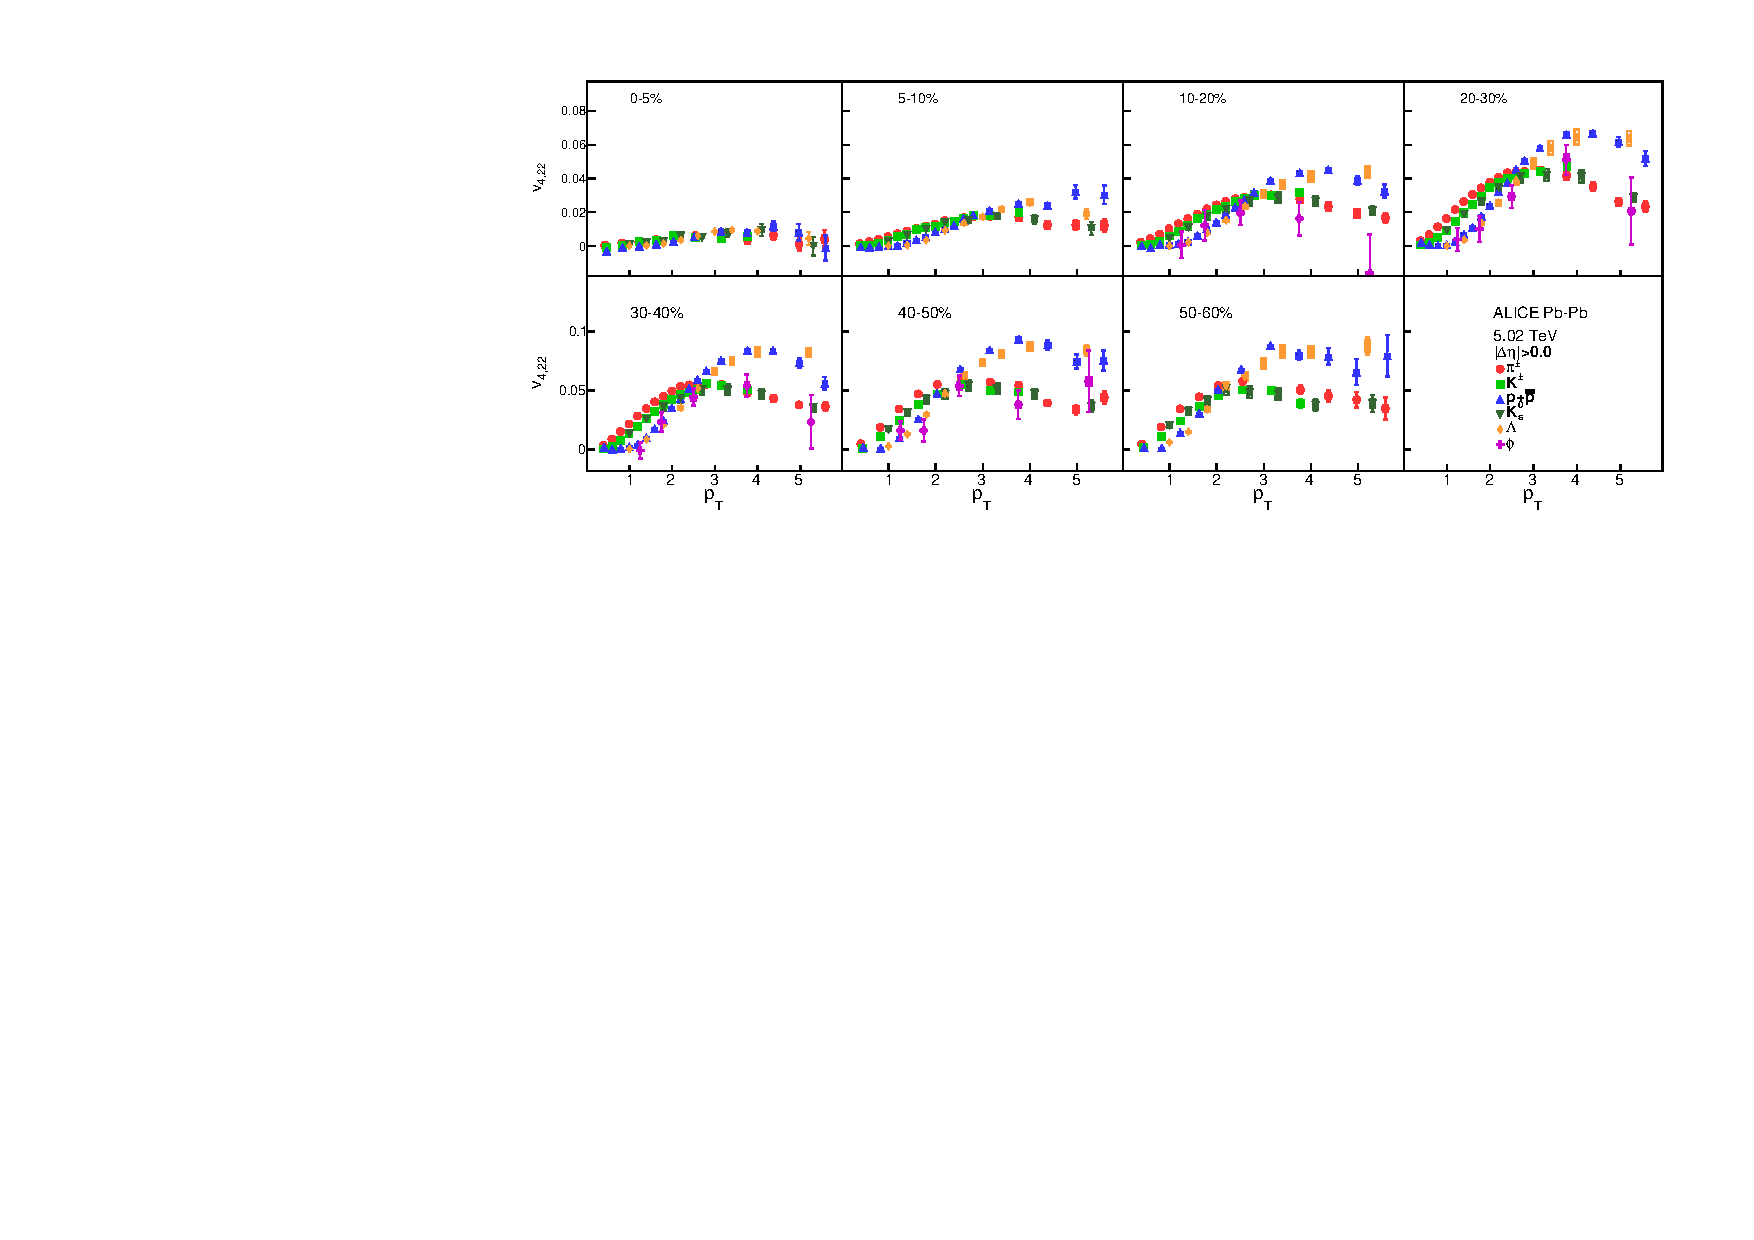
\includegraphics[scale=0.82]{figures/results/All_v422_gap00.pdf}
%DIFDELCMD < %%%
\DIFdelendFL %DIF > 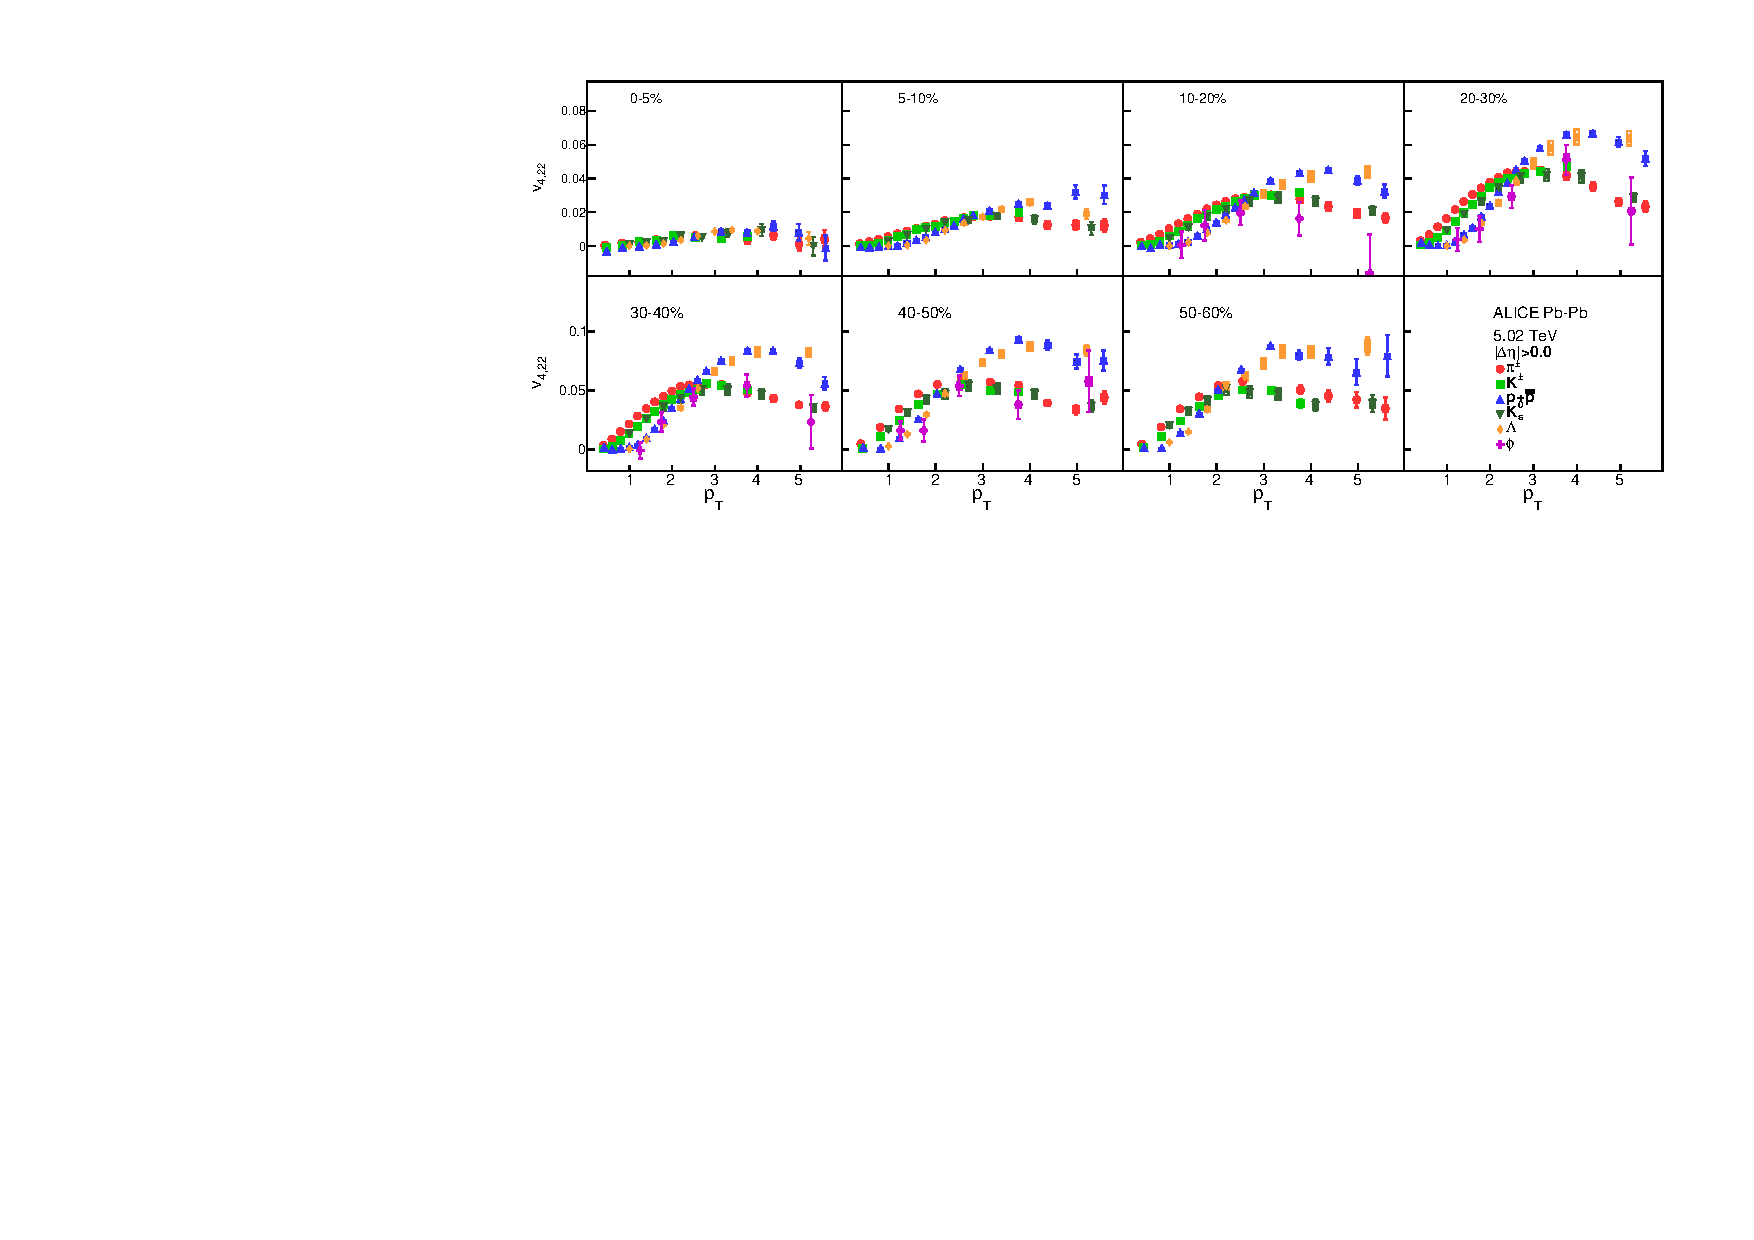
\includegraphics[scale=0.82]{figures/results/All_v422_gap00.pdf}
\DIFaddbeginFL 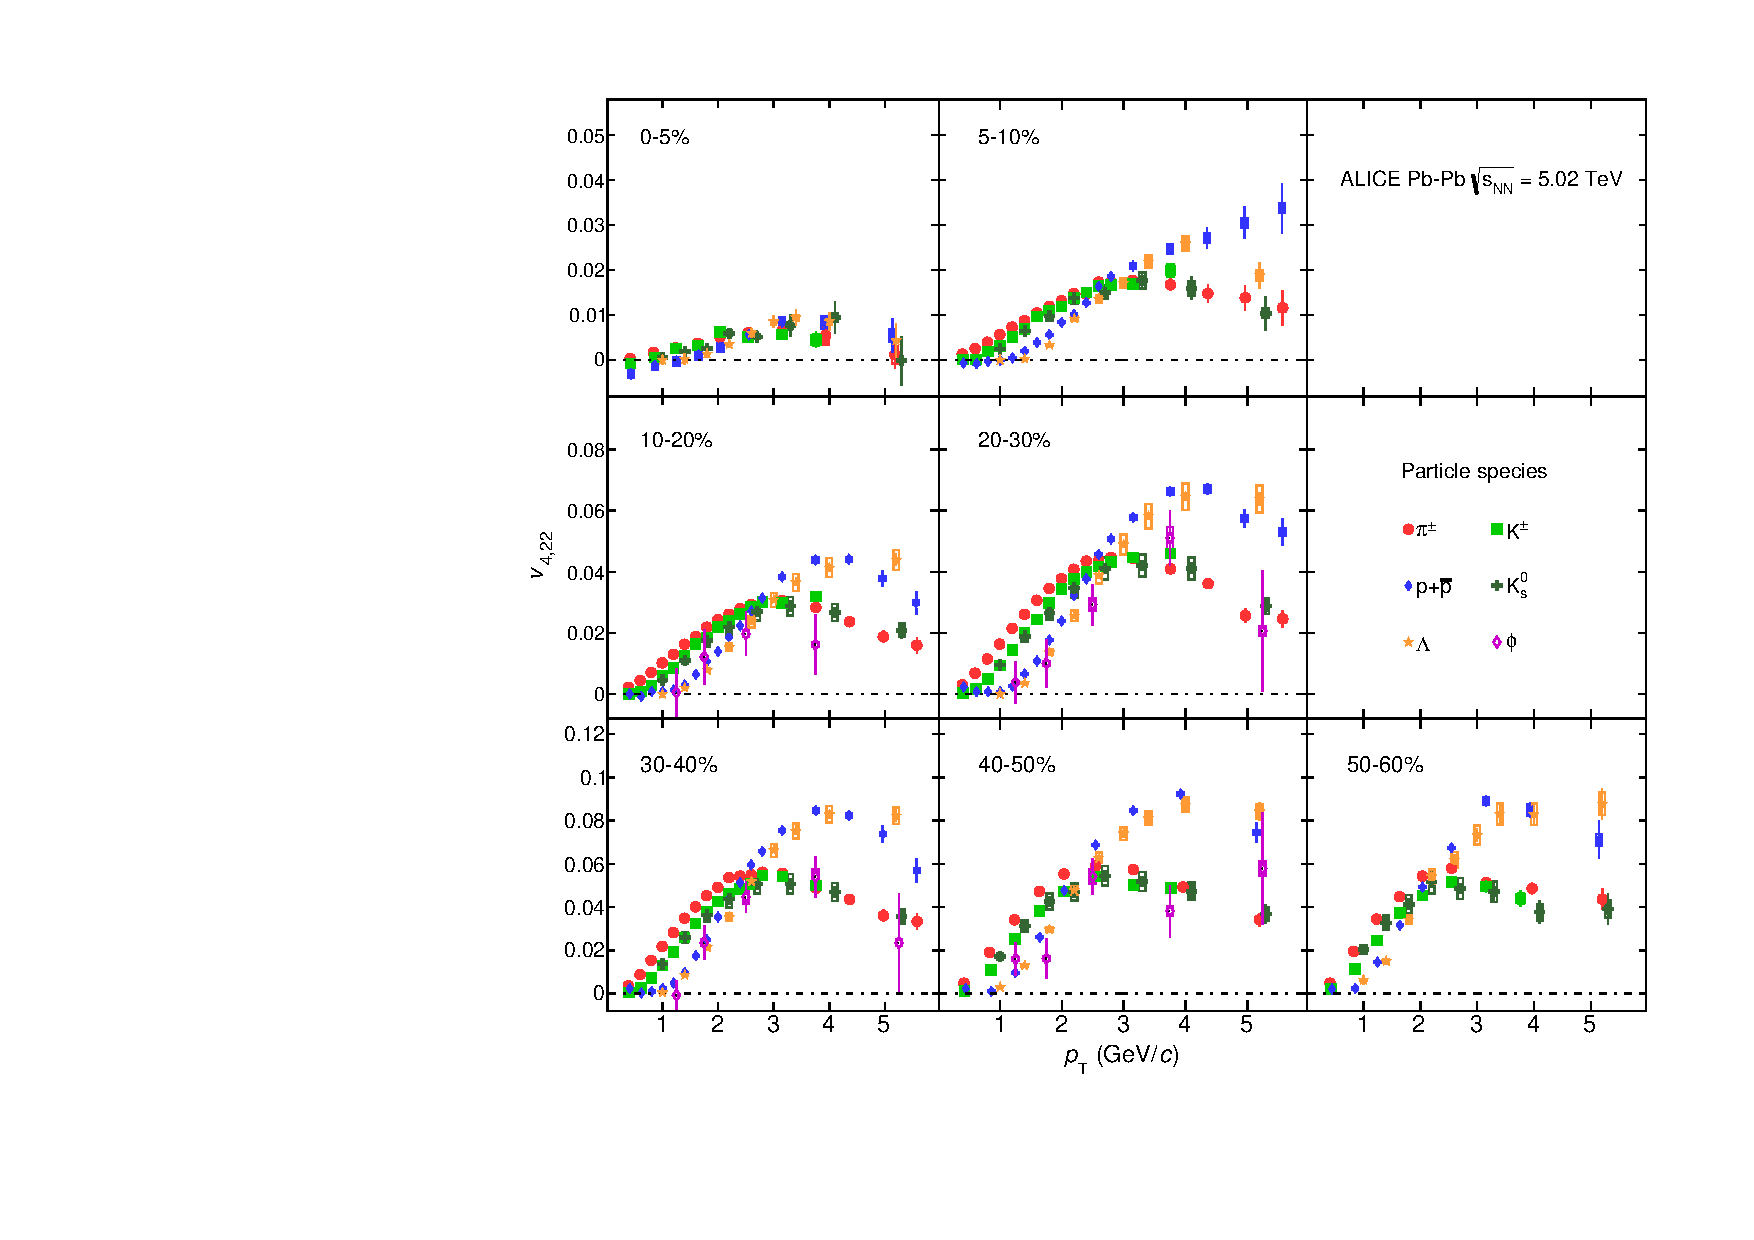
\includegraphics[scale=0.82]{figures/results/All_v422_gap00_PID2_3by3.pdf}
\DIFaddendFL \end{center}
\caption{The \pT-differential $v_{4,22}$ for different particle species grouped into different centrality intervals of Pb--Pb collisions \sNN}
\label{v422_particleDependence}
\end{figure}

Similarly, Figs. \ref{v523_particleDependence}, \ref{v633_particleDependence} and \ref{v6222_particleDependence} show the \pT-differential $v_{5,32}$, $v_{6,33}$ and $v_{6,222}$ respectively, of different particle species for each centrality interval. A clear mass ordering is seen in the low \pT~region, (i.e. \pT $< 2.5$ \GeV), for $v_{5,32}(p_{\rm{T}})$, $v_{6,33}(p_{\rm{T}})$ and $v_{6,222}(p_{\rm{T}})$, which similarly arises from the interplay between the non-linear response of the system and radial flow. 

\begin{figure}[!htb]
\begin{center}
\DIFdelbeginFL %DIFDELCMD < 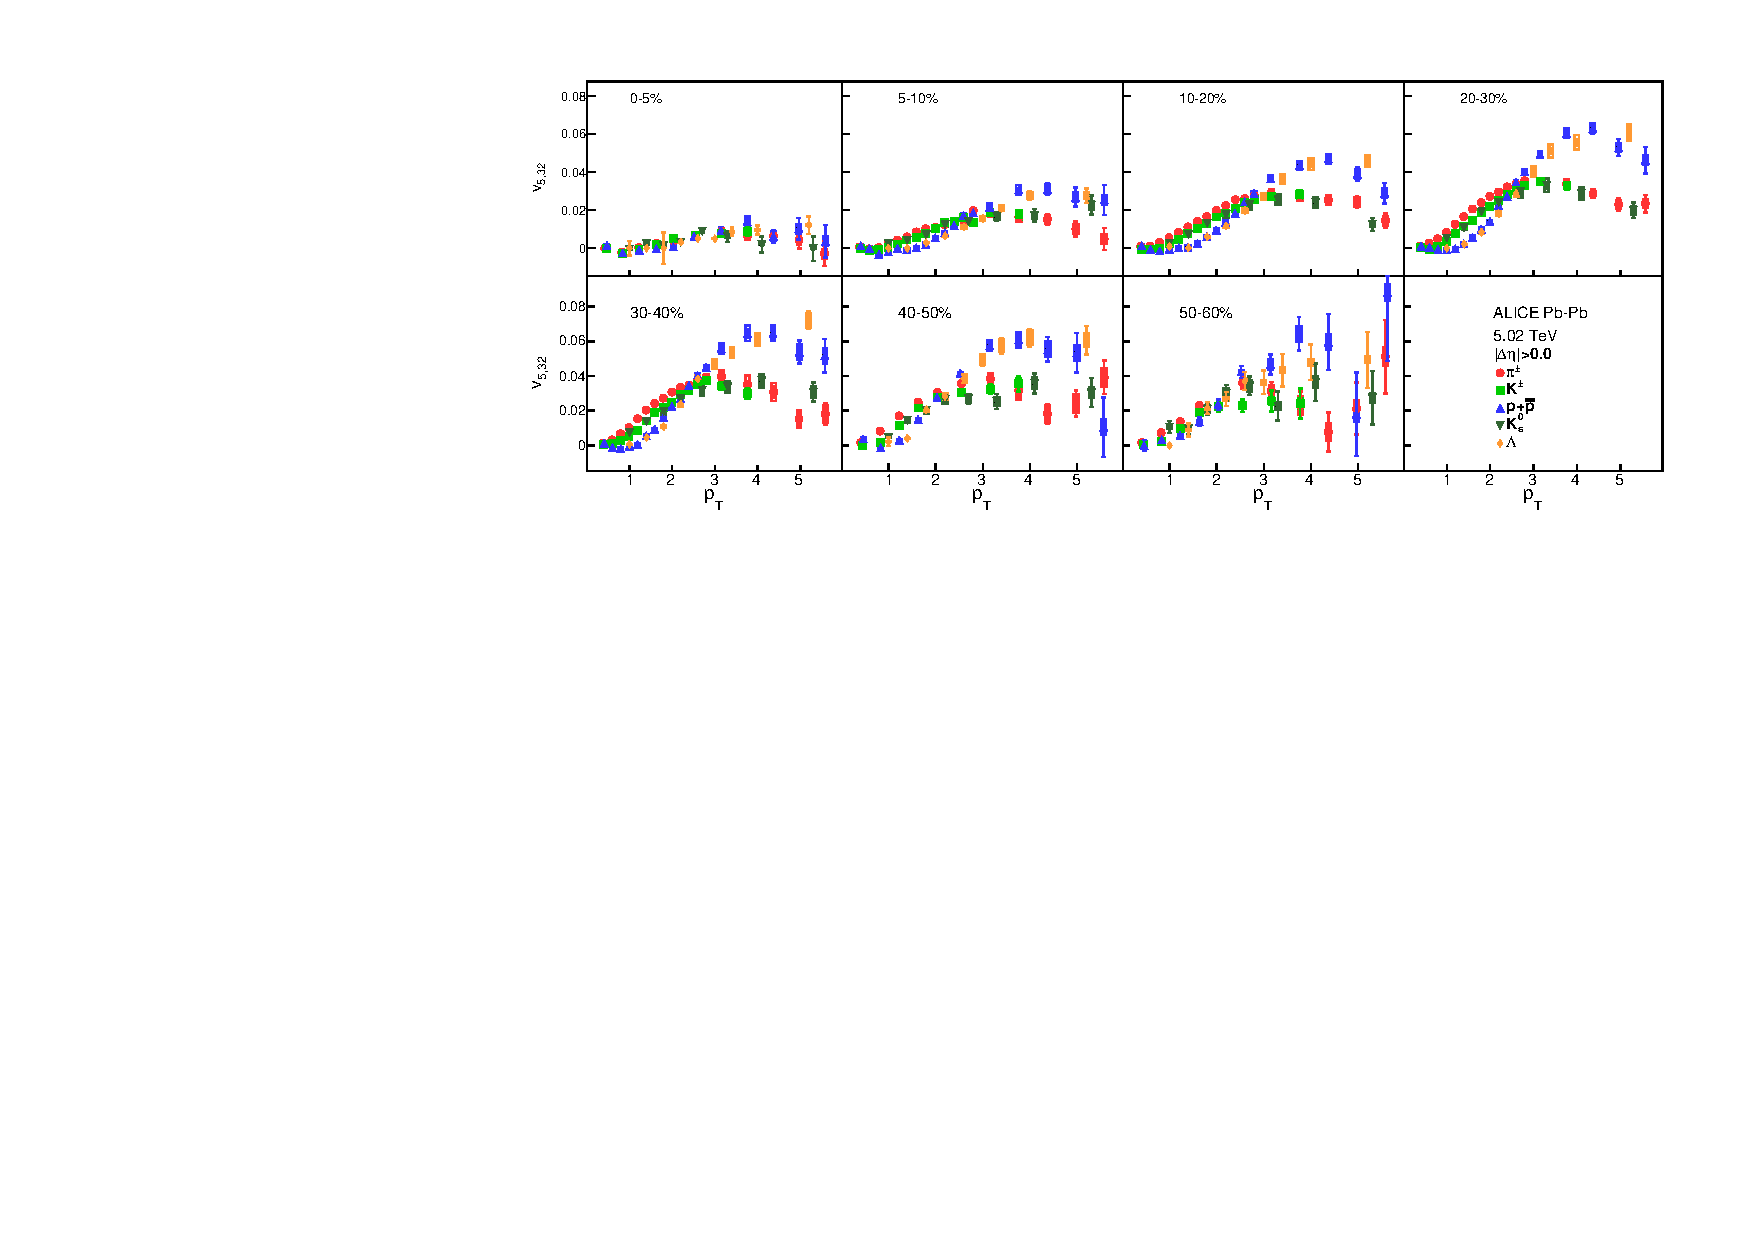
\includegraphics[scale=0.82]{figures/results/All_v523_gap00.pdf}
%DIFDELCMD < %%%
\DIFdelendFL %DIF > 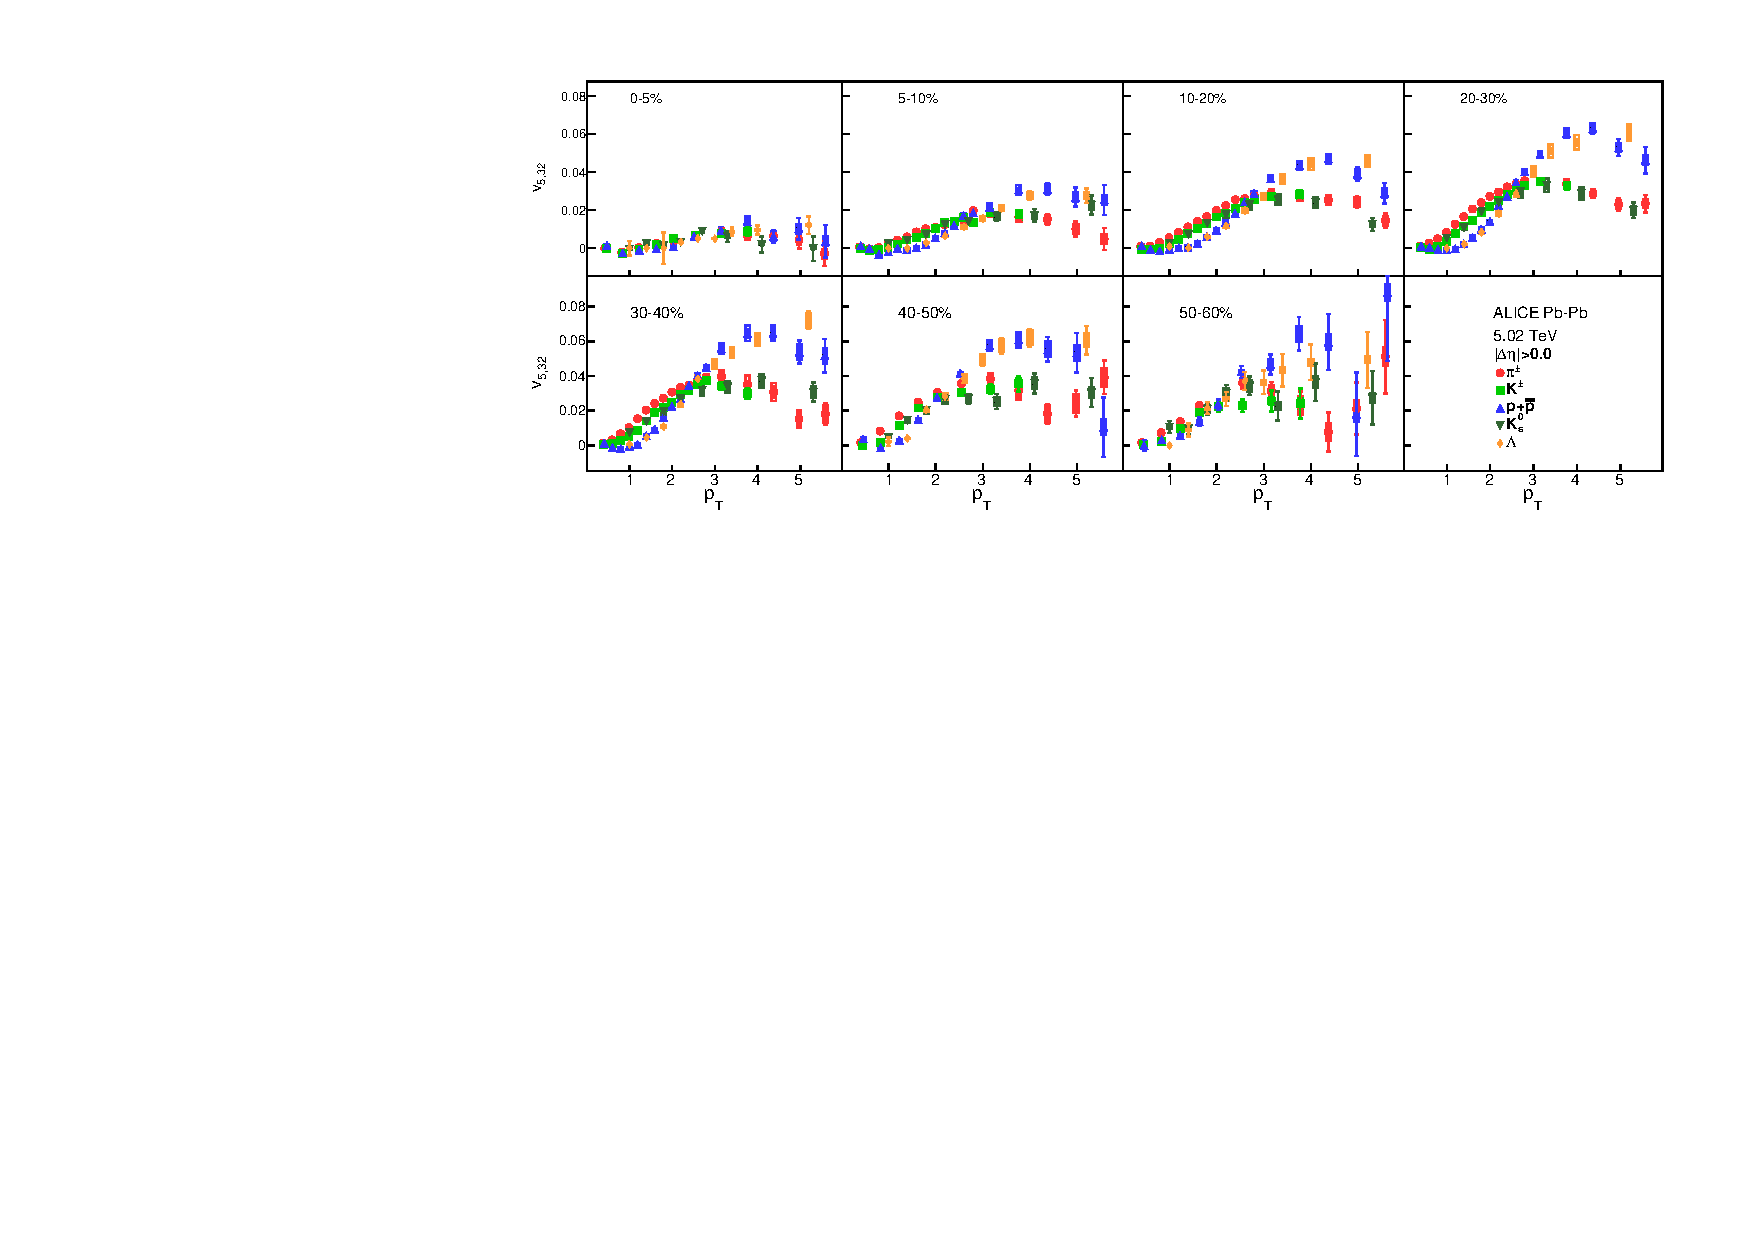
\includegraphics[scale=0.82]{figures/results/All_v523_gap00.pdf}
\DIFaddbeginFL 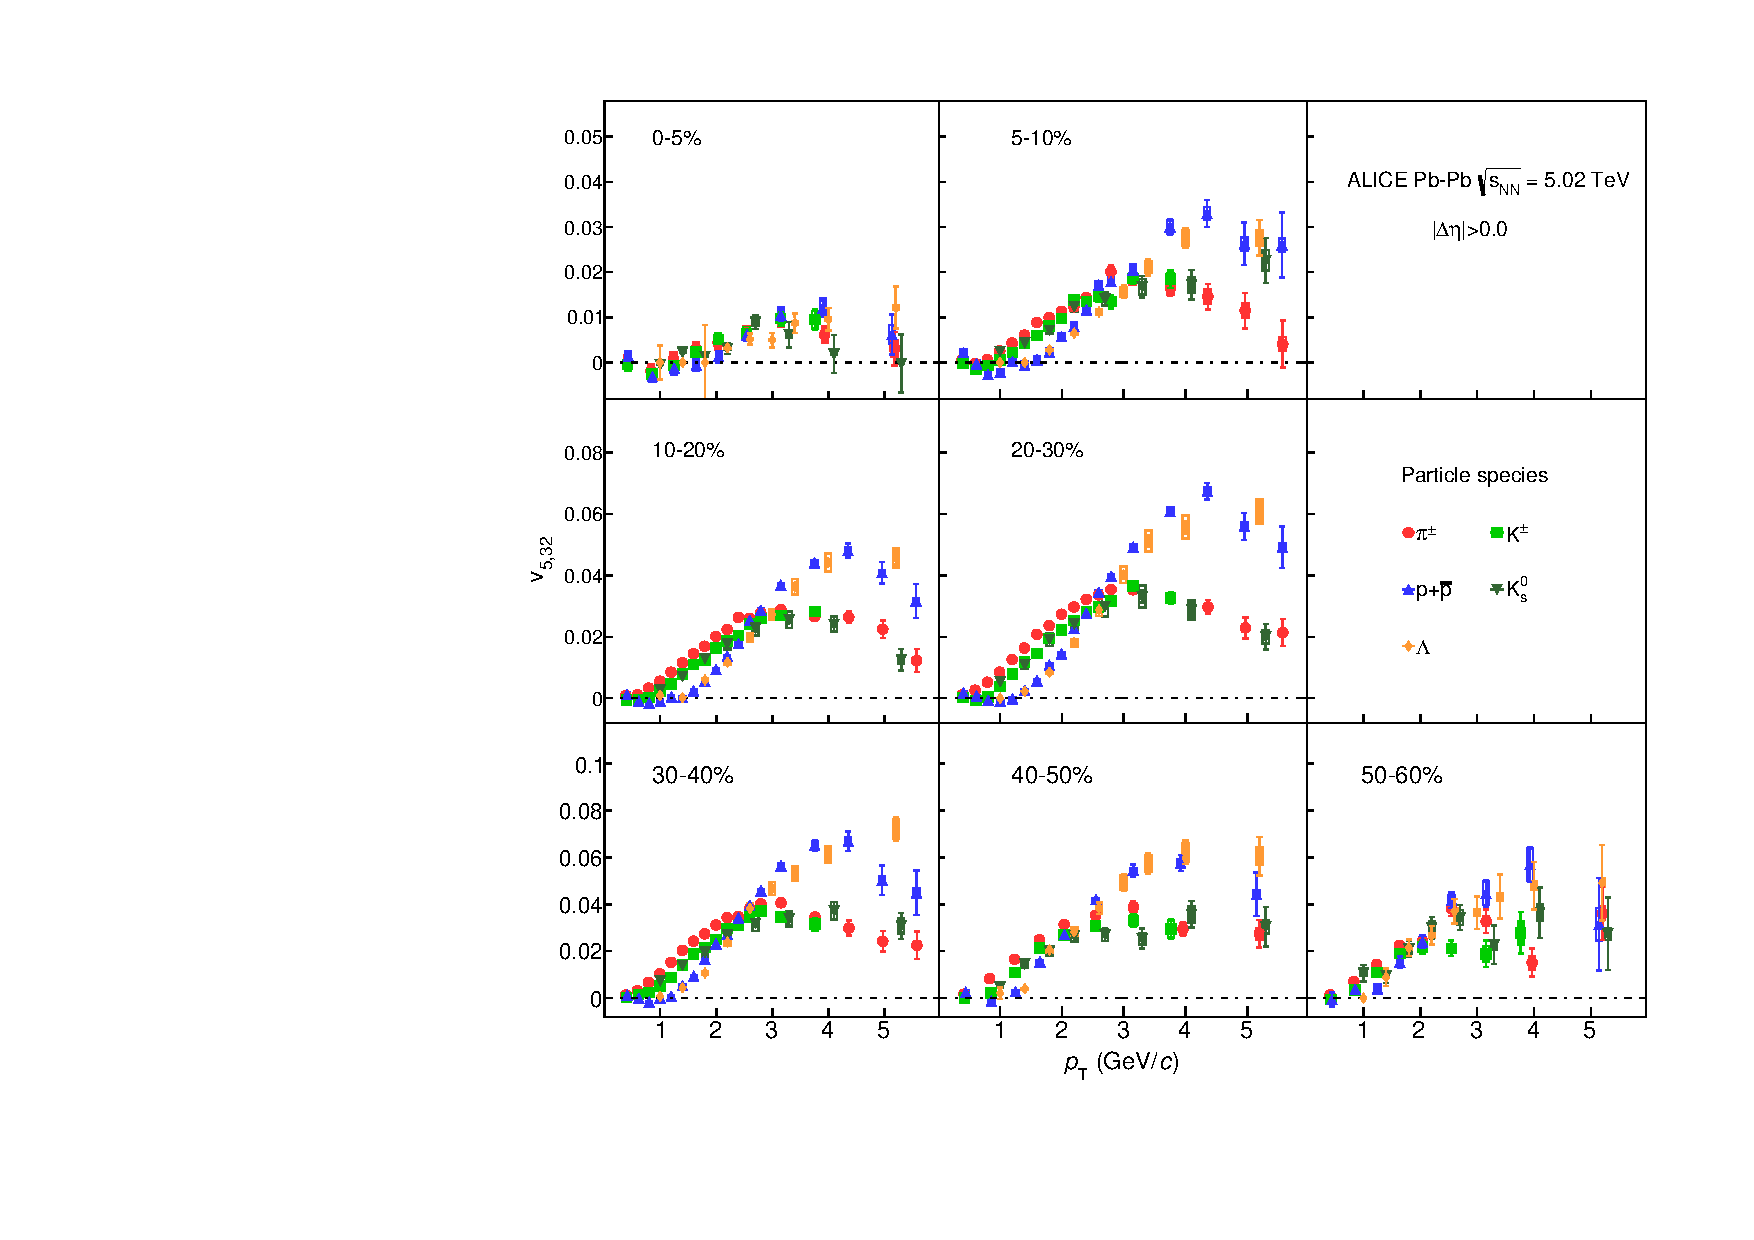
\includegraphics[scale=0.82]{figures/results/All_v523_gap00_PID2_3by3.pdf}

\DIFaddendFL \end{center}
\caption{The \pT-differential $v_{5,32}$ for different particle species grouped into different centrality intervals of Pb--Pb collisions \sNN}
\label{v523_particleDependence}
\end{figure}

\begin{figure}[!htb]
\begin{center}
\DIFdelbeginFL %DIFDELCMD < 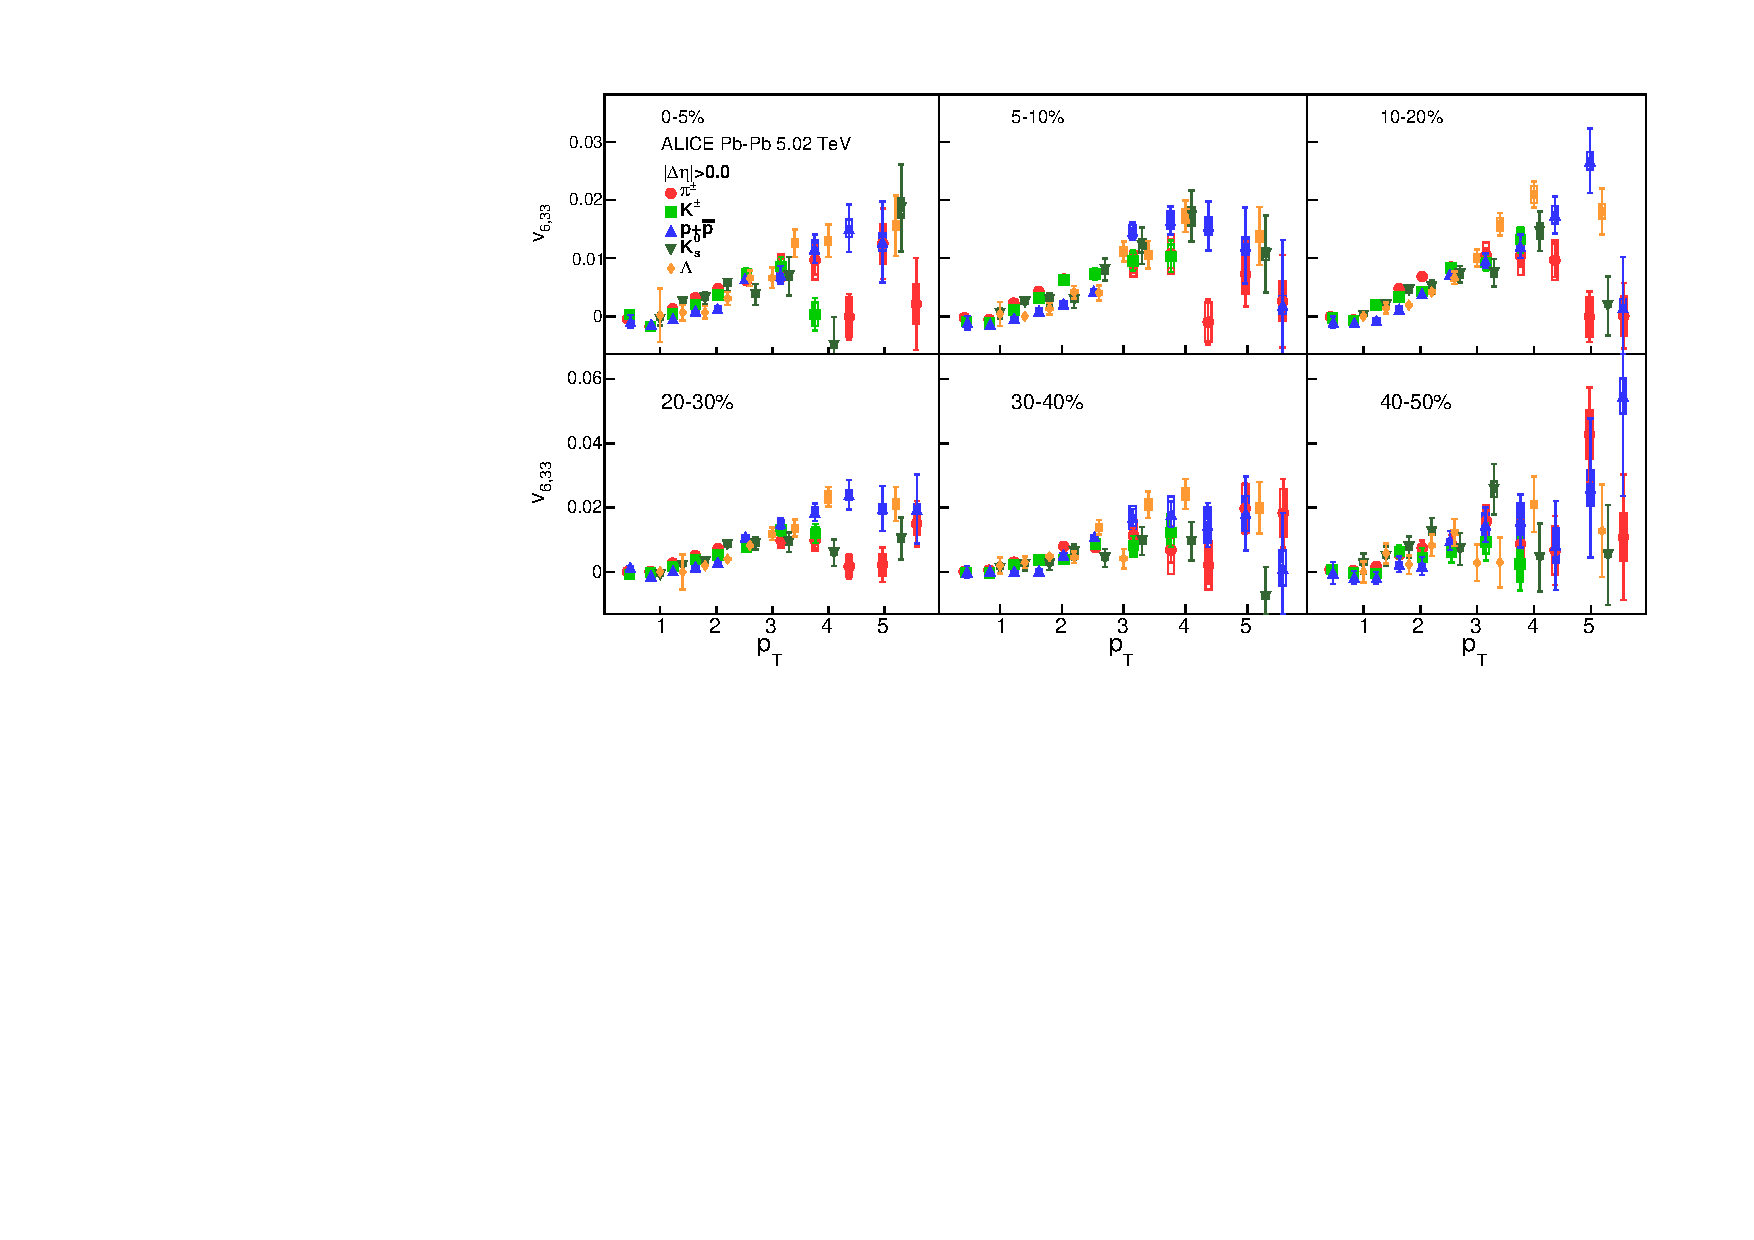
\includegraphics[scale=0.62]{figures/results/All_v633_gap00.pdf}
%DIFDELCMD < %%%
\DIFdelendFL %DIF > 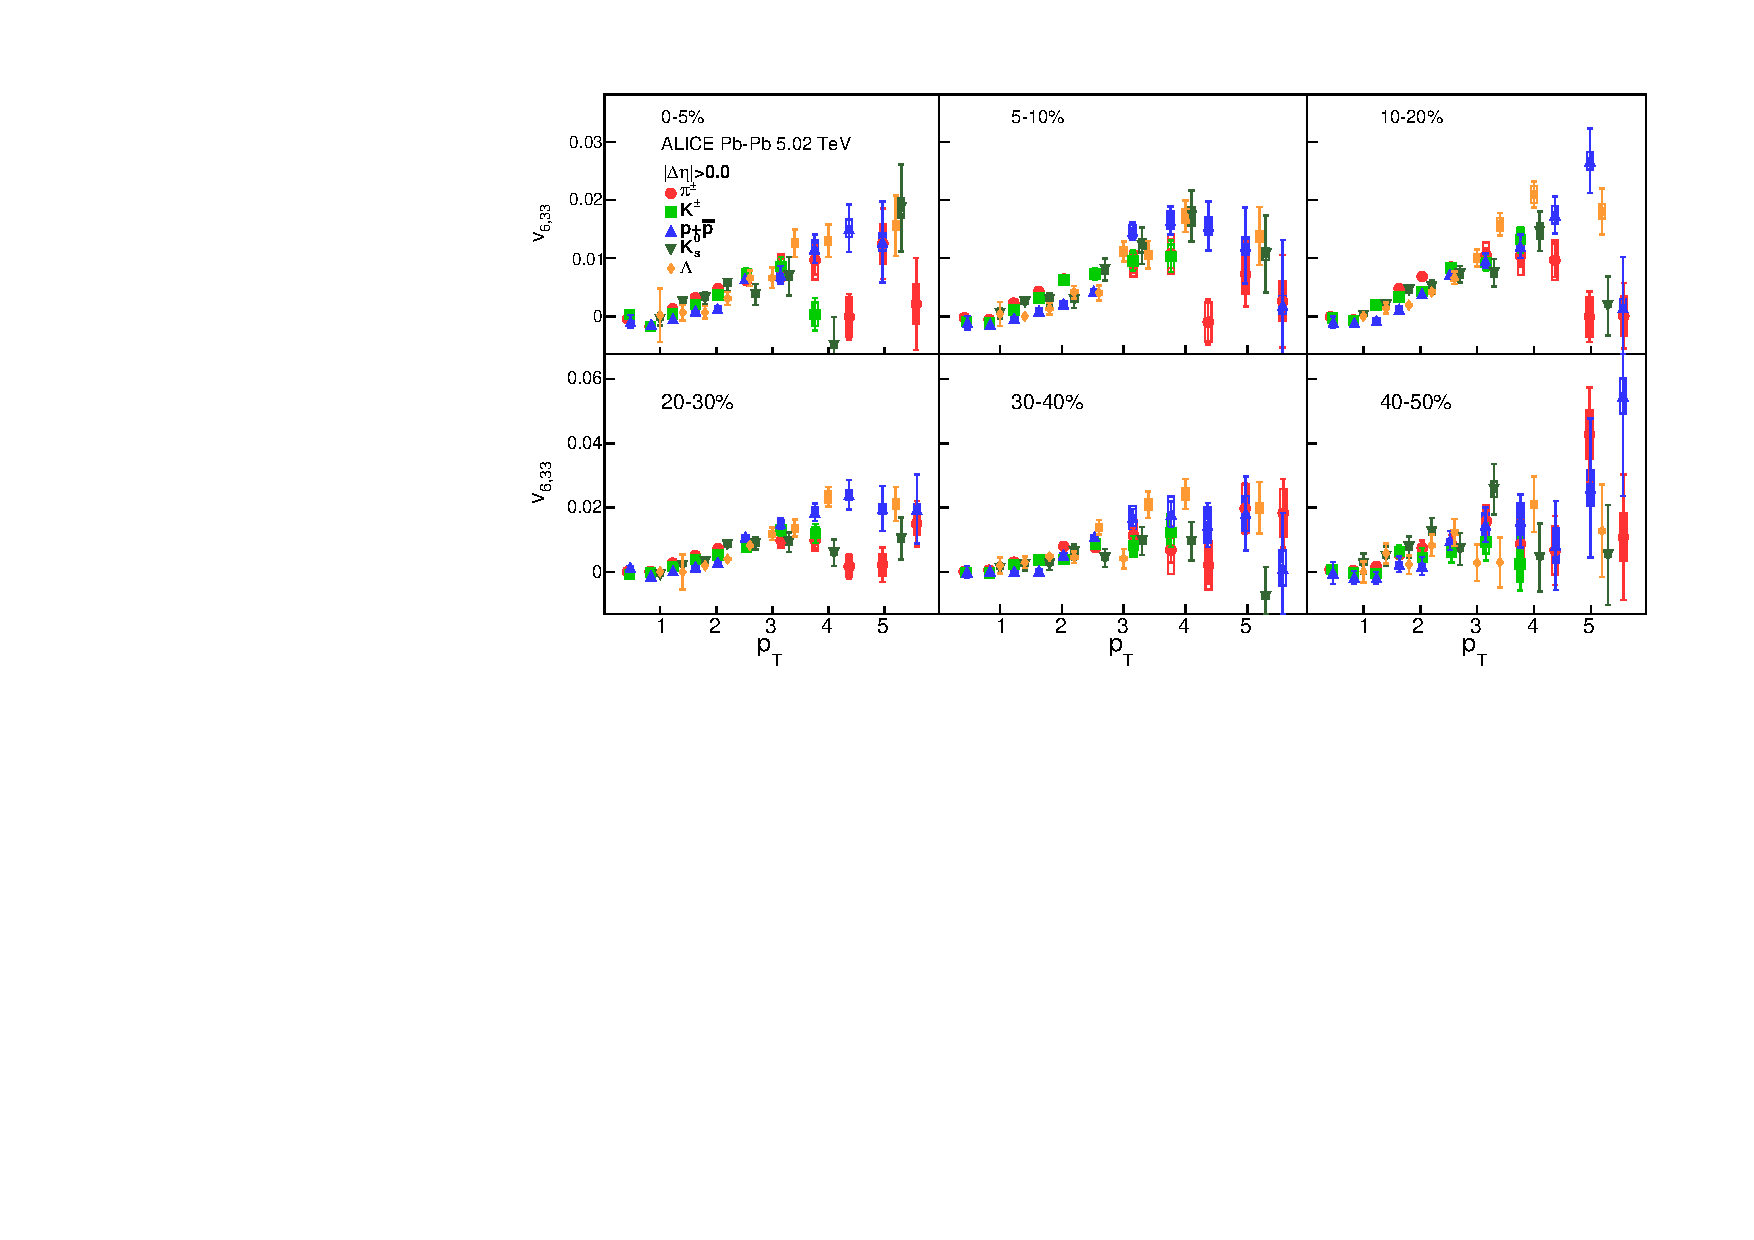
\includegraphics[scale=0.62]{figures/results/All_v633_gap00.pdf}
\DIFaddbeginFL 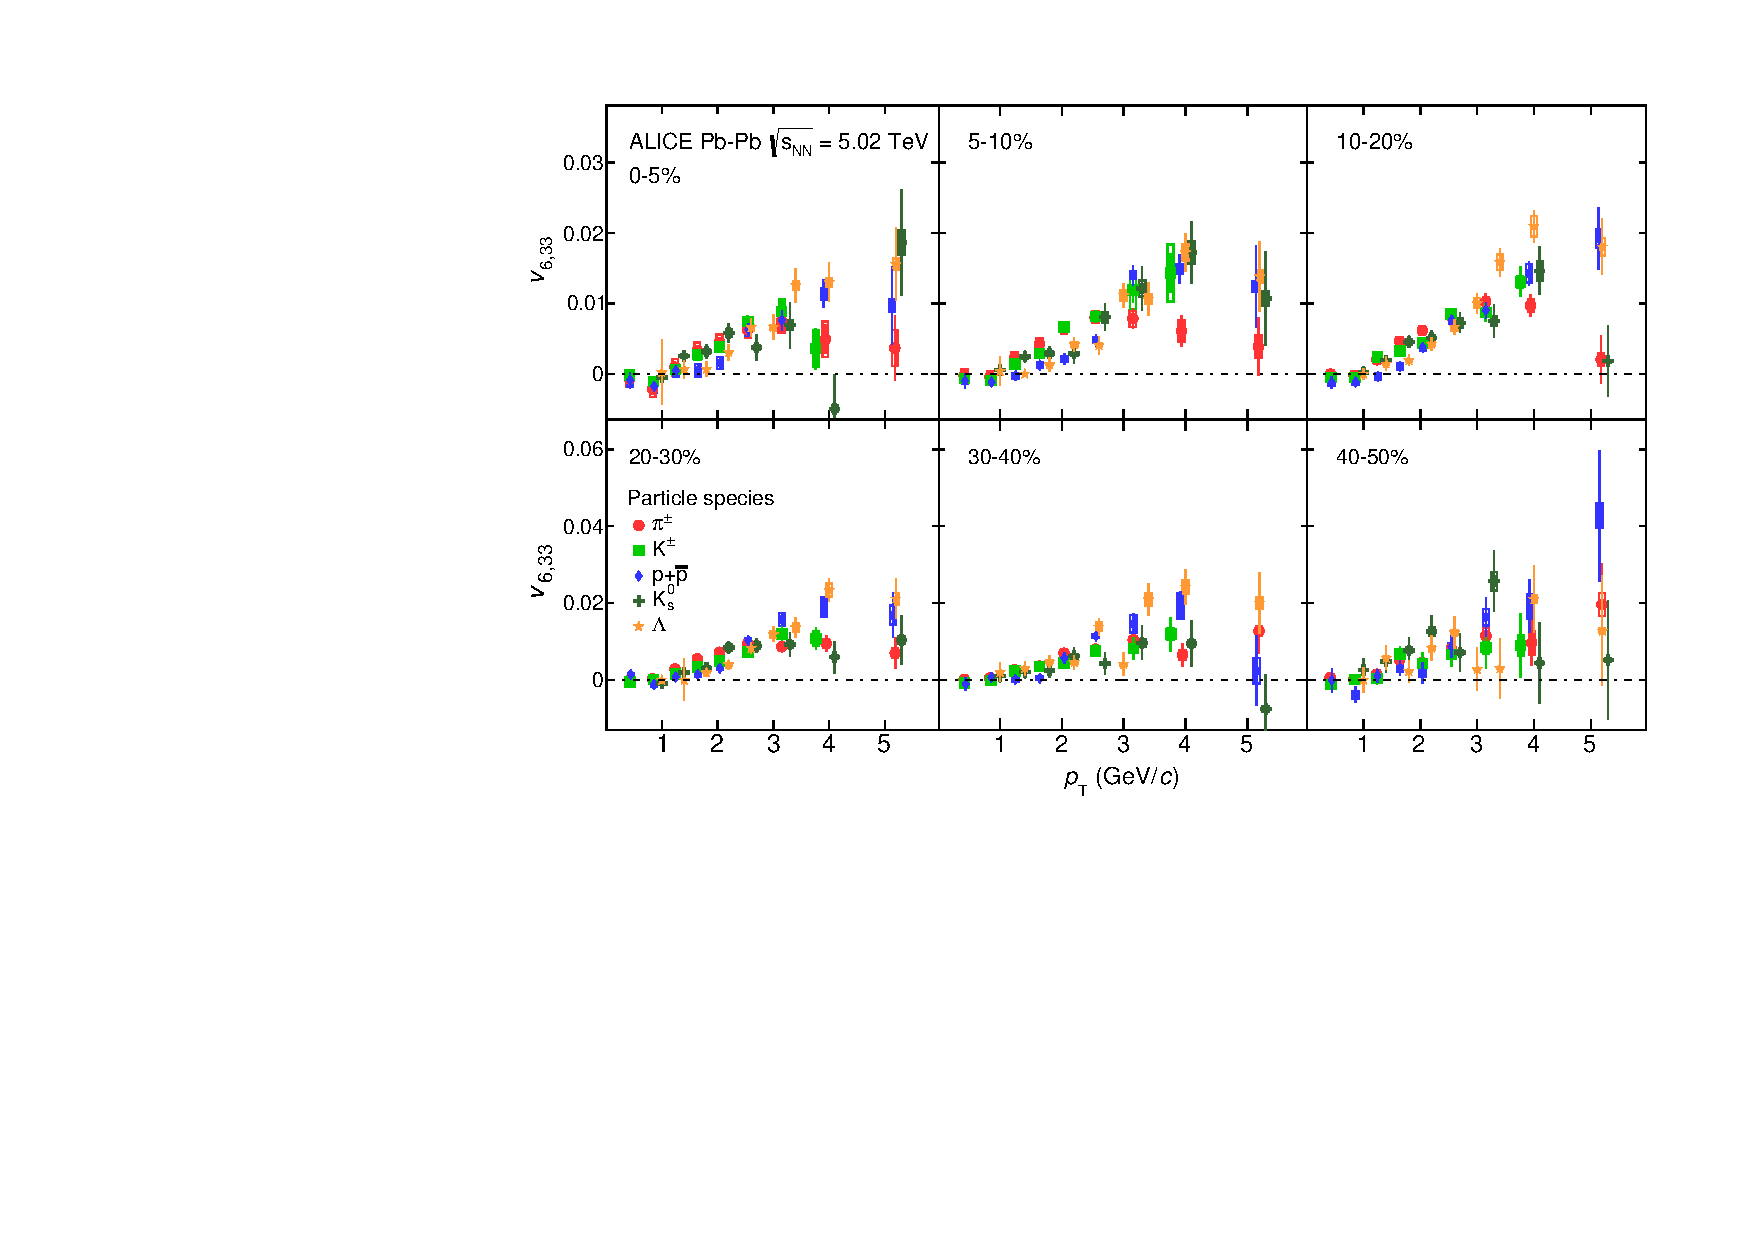
\includegraphics[scale=0.82]{figures/results/All_v633_gap00_PID2_3by2.pdf}

\DIFaddendFL \end{center}
\caption{The \pT-differential $v_{6,33}$ for different particle species grouped into different centrality intervals of Pb--Pb collisions \sNN}
\label{v633_particleDependence}
\end{figure}

\begin{figure}[!htb]
\begin{center}
\DIFdelbeginFL %DIFDELCMD < 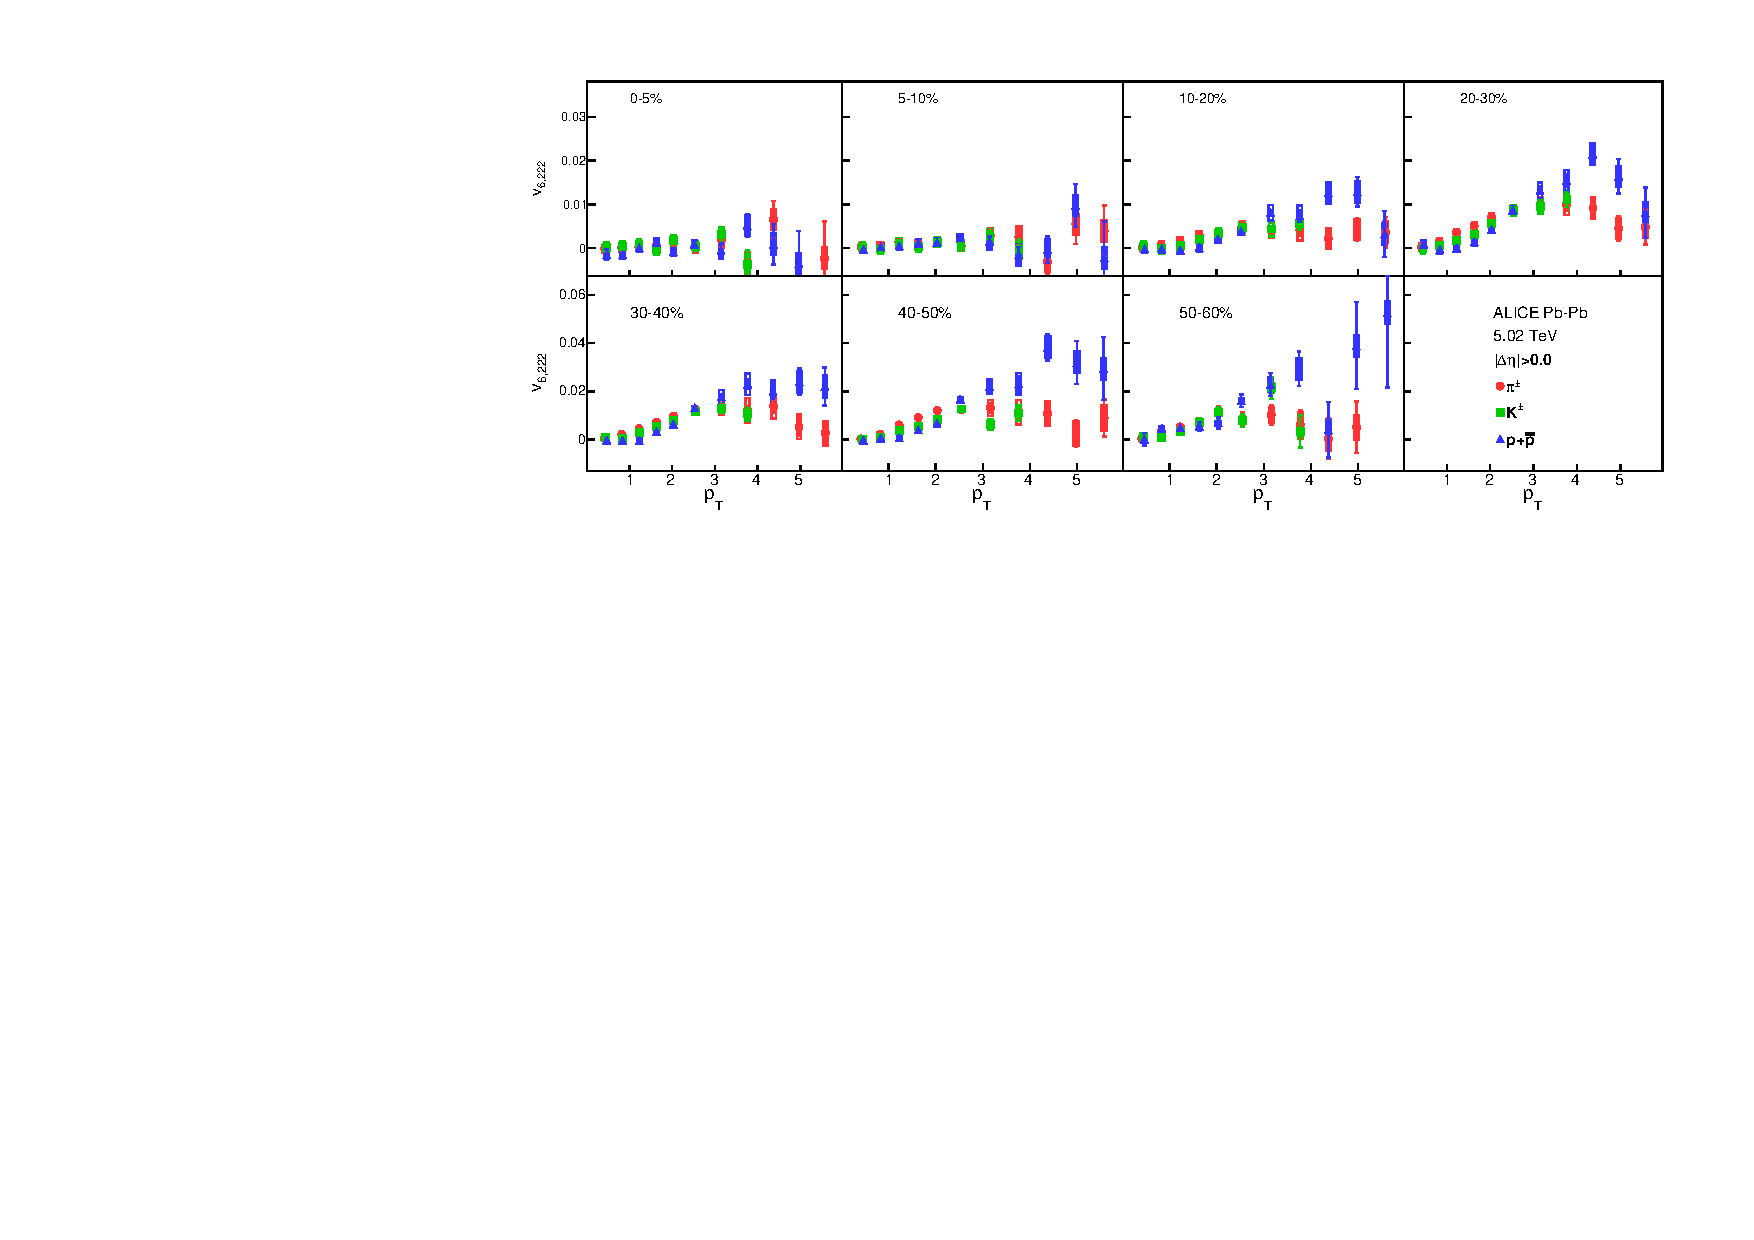
\includegraphics[scale=0.82]{figures/results/All_v6222_gap00.pdf}
%DIFDELCMD < %%%
\DIFdelendFL %DIF > 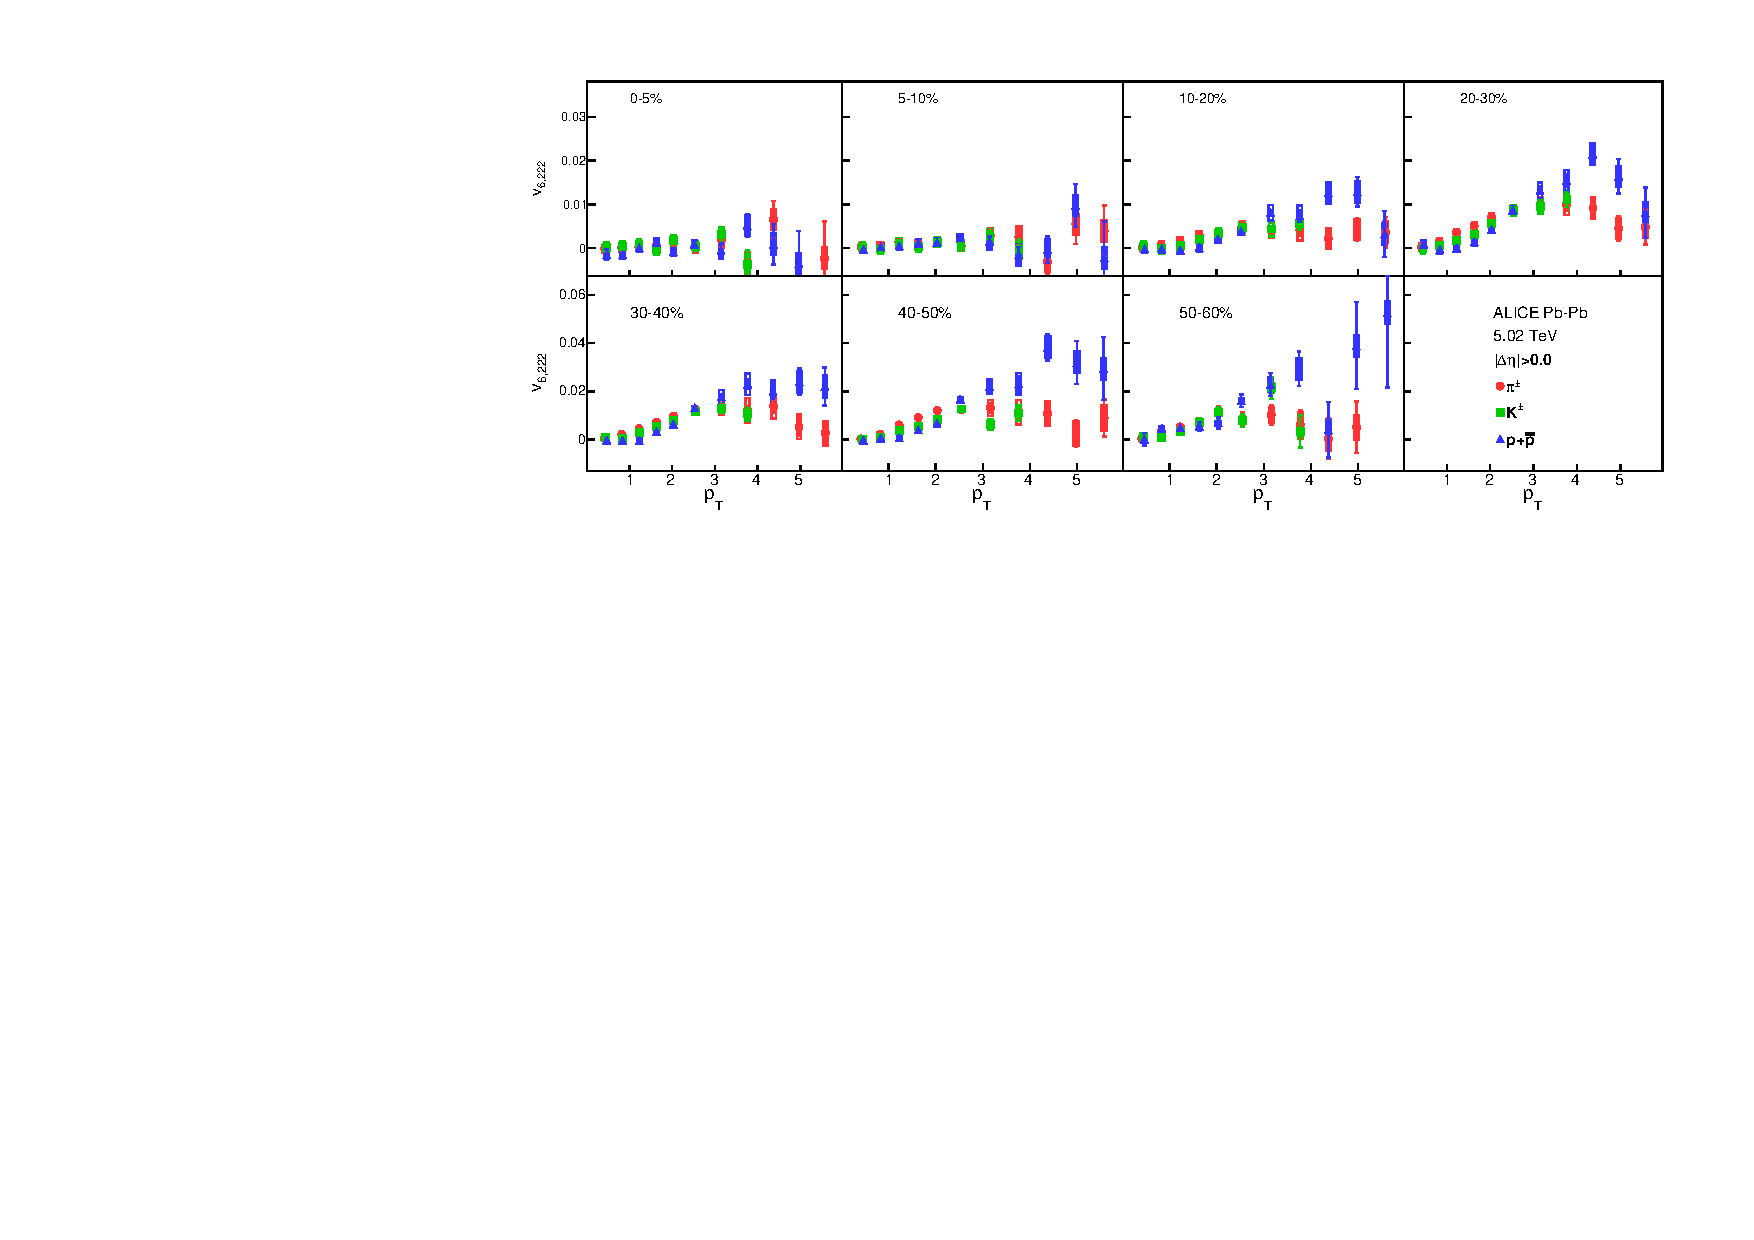
\includegraphics[scale=0.82]{figures/results/All_v6222_gap00.pdf}
\DIFaddbeginFL 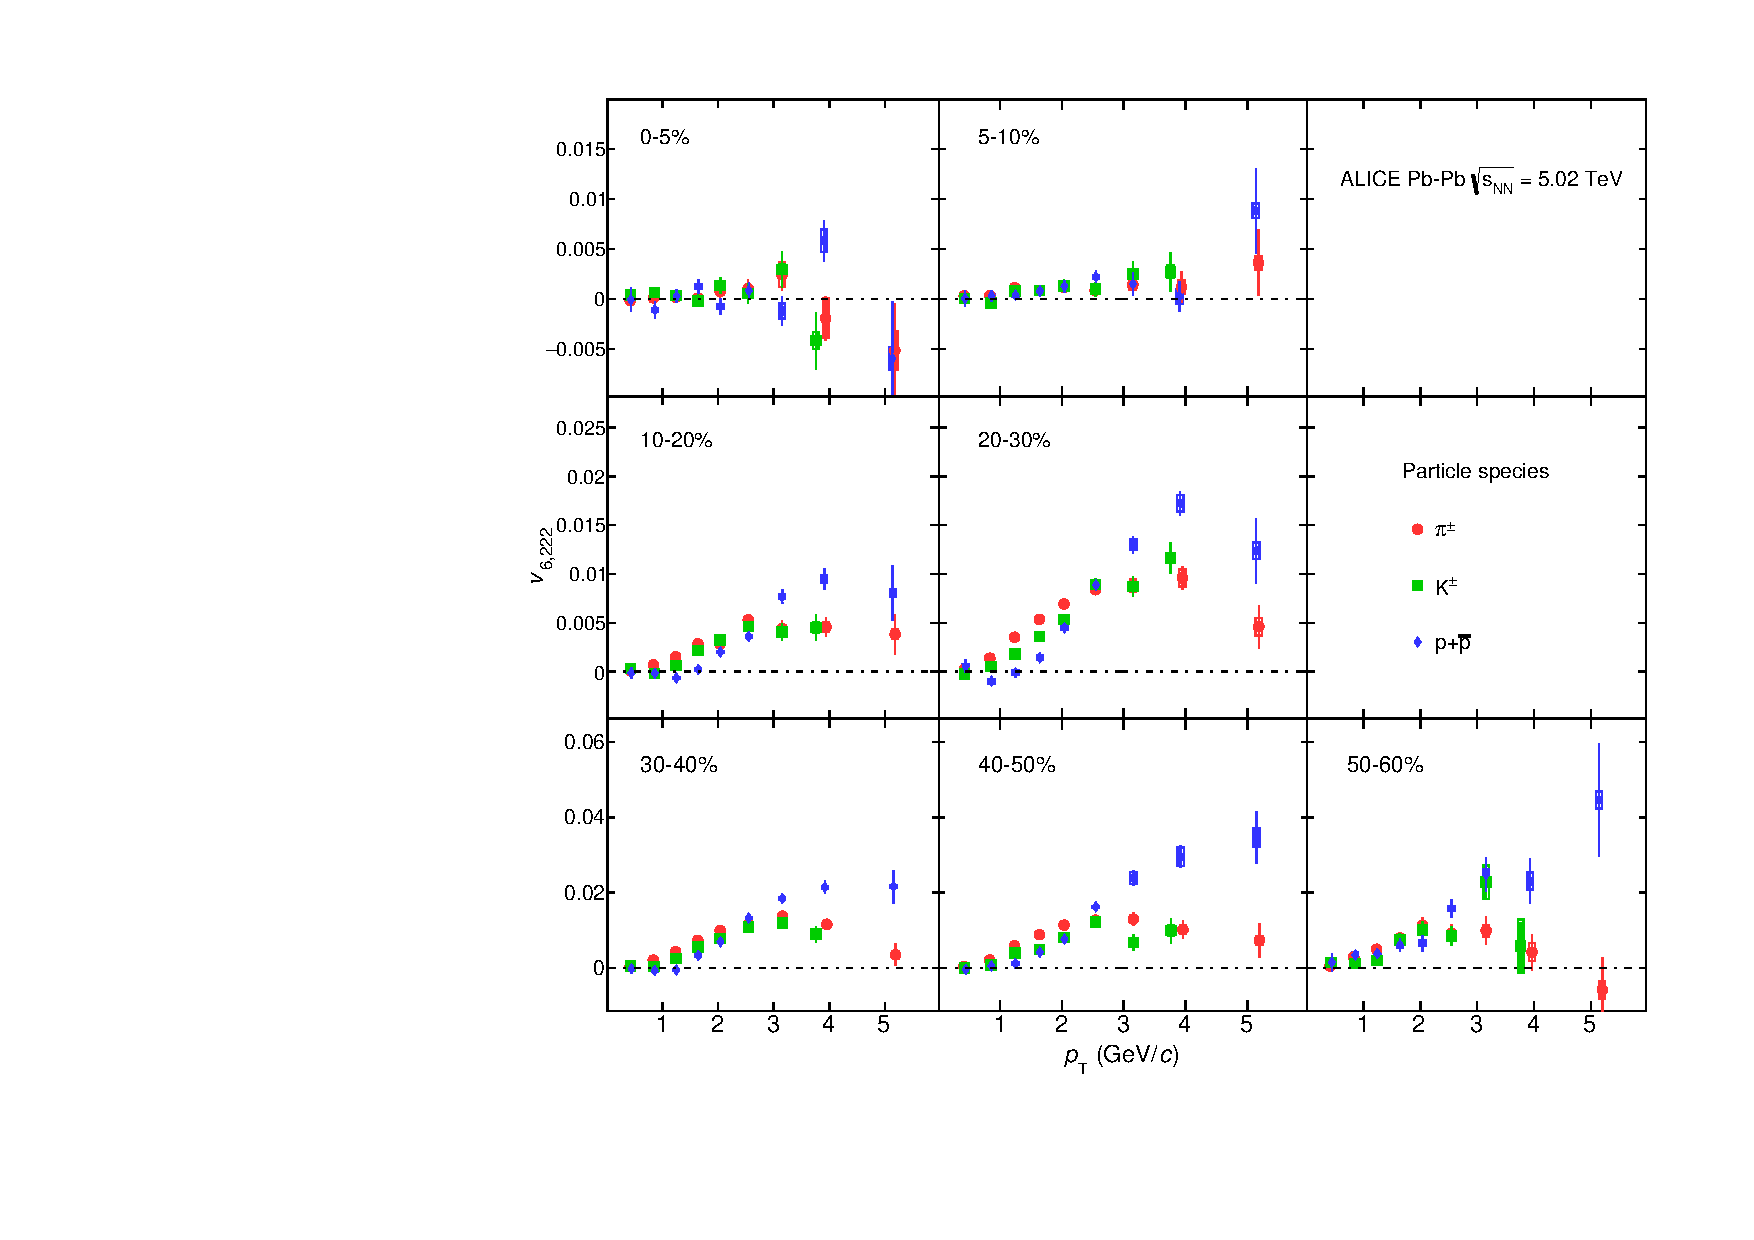
\includegraphics[scale=0.82]{figures/results/All_v6222_gap00_PID2_3by3.pdf}

\DIFaddendFL \end{center}
\caption{The \pT-differential $v_{6,222}$ for different particle species grouped into different centrality intervals of Pb--Pb collisions \sNN}
\label{v6222_particleDependence}
\end{figure}

\newpage

In addition, in the intermediate \pT~region (for \pT $> 2.5$ \GeV) the data points of Figs. \ref{v422_particleDependence}-\ref{v6222_particleDependence} exhibit a particle type grouping. In particular, mesons (\pion, \kaon, \Ks~and $\phi$) and baryons (\proton~and \lambdas) group based on their type with $v_{n,mk}$ of baryons having a larger magnitude. This particle type grouping was previously seen in the anisotropic flow measurements \cite{Abelev:2014pua,Adam:2016nfo,Acharya:2018zuq,Adams:2003am,Abelev:2007qg,Adler:2003kt,Adare:2006ti} \DIFaddbegin \DIFadd{of various particle species }\DIFaddend triggering the development of calculations relying on coalescence. \DIFaddbegin \DIFadd{This suggests that flow develops at the parsonic stage and if so, combining two or three quarks to form hadronic states might result into hadrons inheriting the transverse momentum and subsequently, $v_{n}$ of their constituents. }\DIFaddend As a next step it was suggested to use a form of number of constituent quark (NCQ) scaling in which both flow coefficients and \pT~were scaled by the number of constituent quarks ($n_{q}$). This scaling, worked initially at RHIC energies, although later measurements revealed sizeable deviations from a perfect scaling \cite{Adams:2003am,Abelev:2007qg,Adler:2003kt,Adare:2006ti}. Recently, ALICE measurements showed that the NCQ scaling at LHC energies holds at best at an approximate level of 20\% for $v_{n}$ \cite{Abelev:2014pua,Adam:2016nfo,Acharya:2018zuq}. Various theoretical ideas were created to address the origin of possible scaling by requiring quark coalescence to be the dominant particle production mechanism in the intermediate \pT~region, where the hydrodynamic evolution of the fireball is not the driving force behind the development of anisotropic flow \cite{Voloshin:2002wa,Molnar:2003ff}.

\DIFdelbegin \subsection{\DIFdel{Test of scaling properties}}
%DIFAUXCMD
\addtocounter{subsection}{-1}%DIFAUXCMD
%DIFDELCMD < \label{subsection:NCQscaling}
%DIFDELCMD < %%%
\DIFdelend %DIF > \subsection{Test of scaling properties}
%DIF > \label{subsection:NCQscaling}

Figures \ref{v422_NCQ}, \ref{v523_NCQ}, \ref{v633_NCQ} and \ref{v6222_NCQ} present $v_{4,22}$, $v_{5,32}$, $v_{6,33}$ and $v_{6,222}$ respectively, scaled by the inverse of number of constituent quarks ($n_{q}$) as a function of \pTnq~for \pion, \kaon, \proton, \Ks, \lambdas~and $\phi$-meson grouped in different centrality intervals. The scaling is consistent with the observations reported for higher order total flow coefficients \cite{Acharya:2018zuq}. Similarly, for non-linear modes this scaling hold at best at an approximate level ($\pm$20\%). 

\begin{figure}[!htb]
\begin{center}
\DIFdelbeginFL %DIFDELCMD < 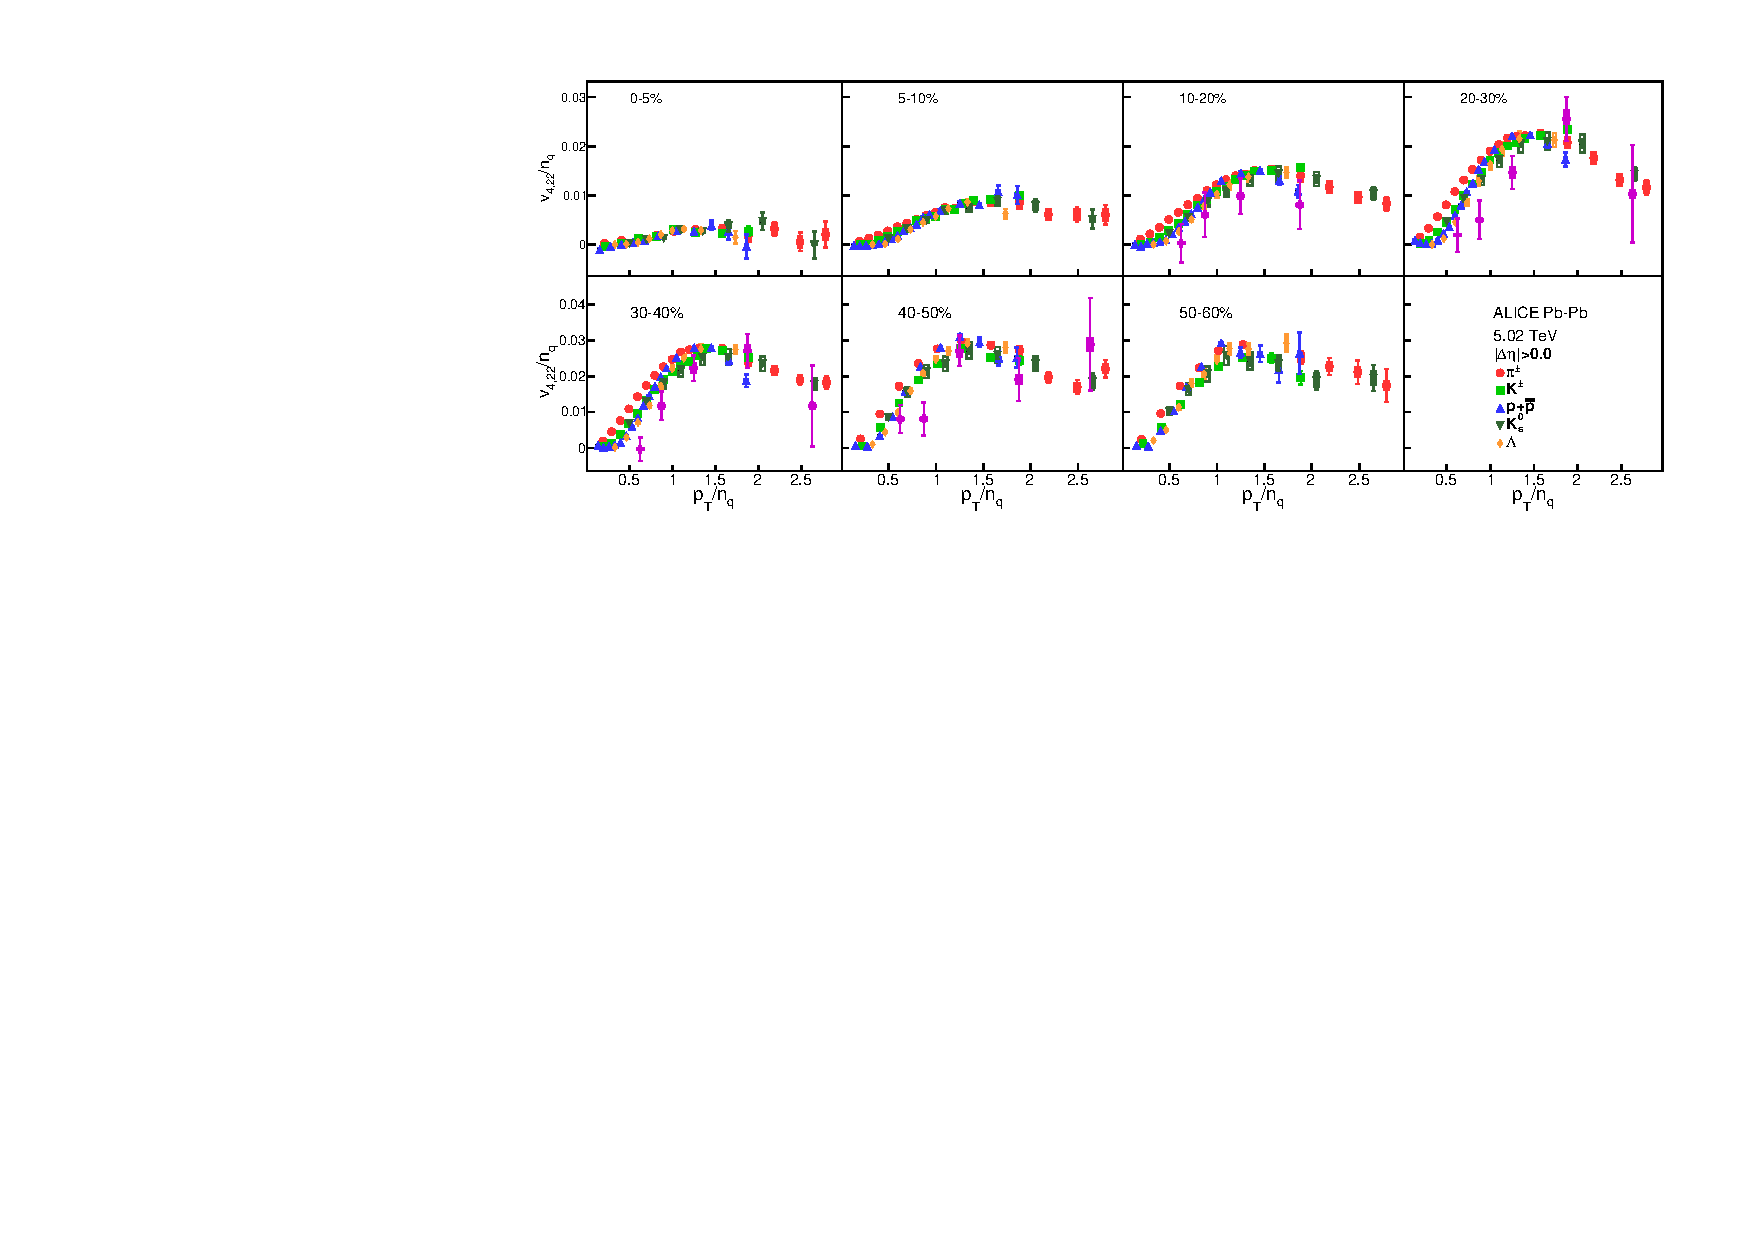
\includegraphics[scale=0.82]{figures/scaling/All_v422_gap00_NCQ.pdf}
%DIFDELCMD < %%%
\DIFdelendFL %DIF > 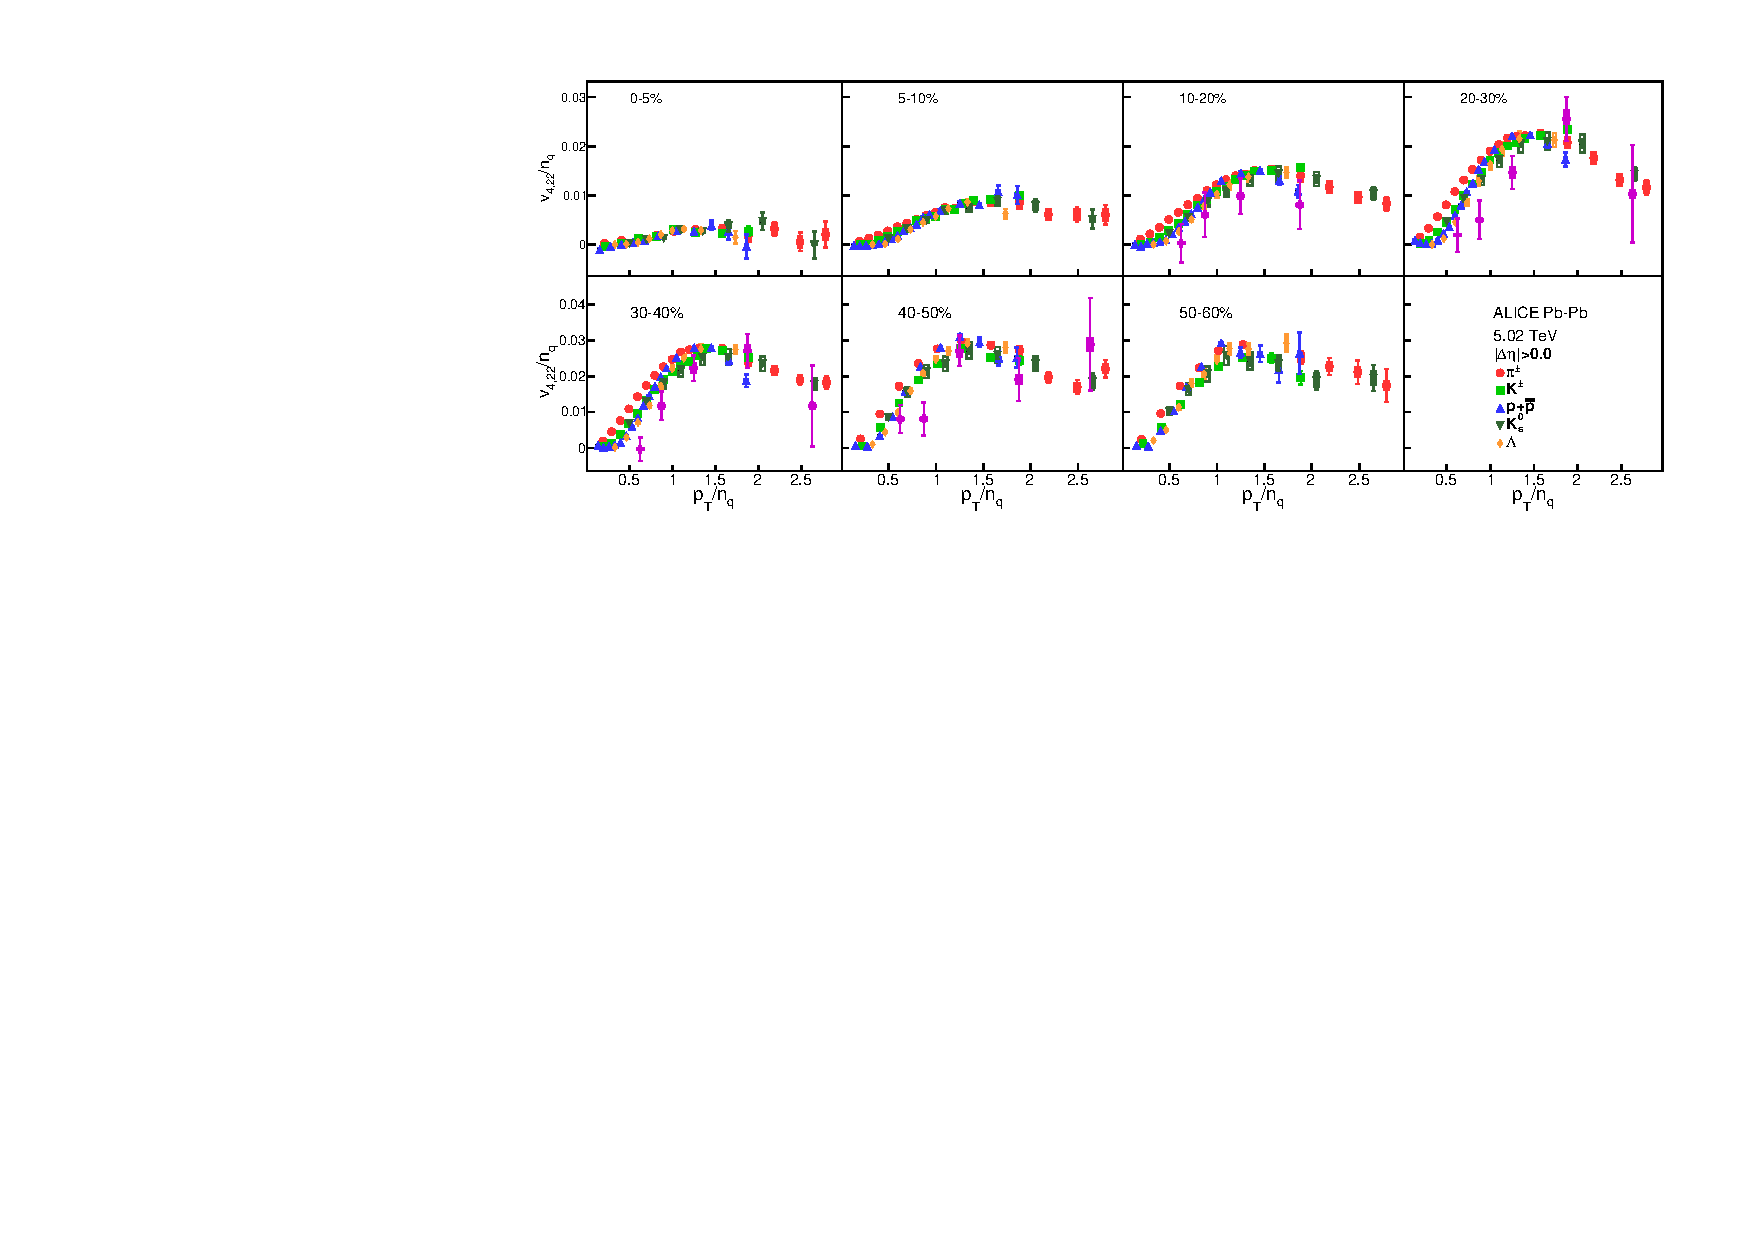
\includegraphics[scale=0.82]{figures/scaling/All_v422_gap00_NCQ.pdf}
\DIFaddbeginFL 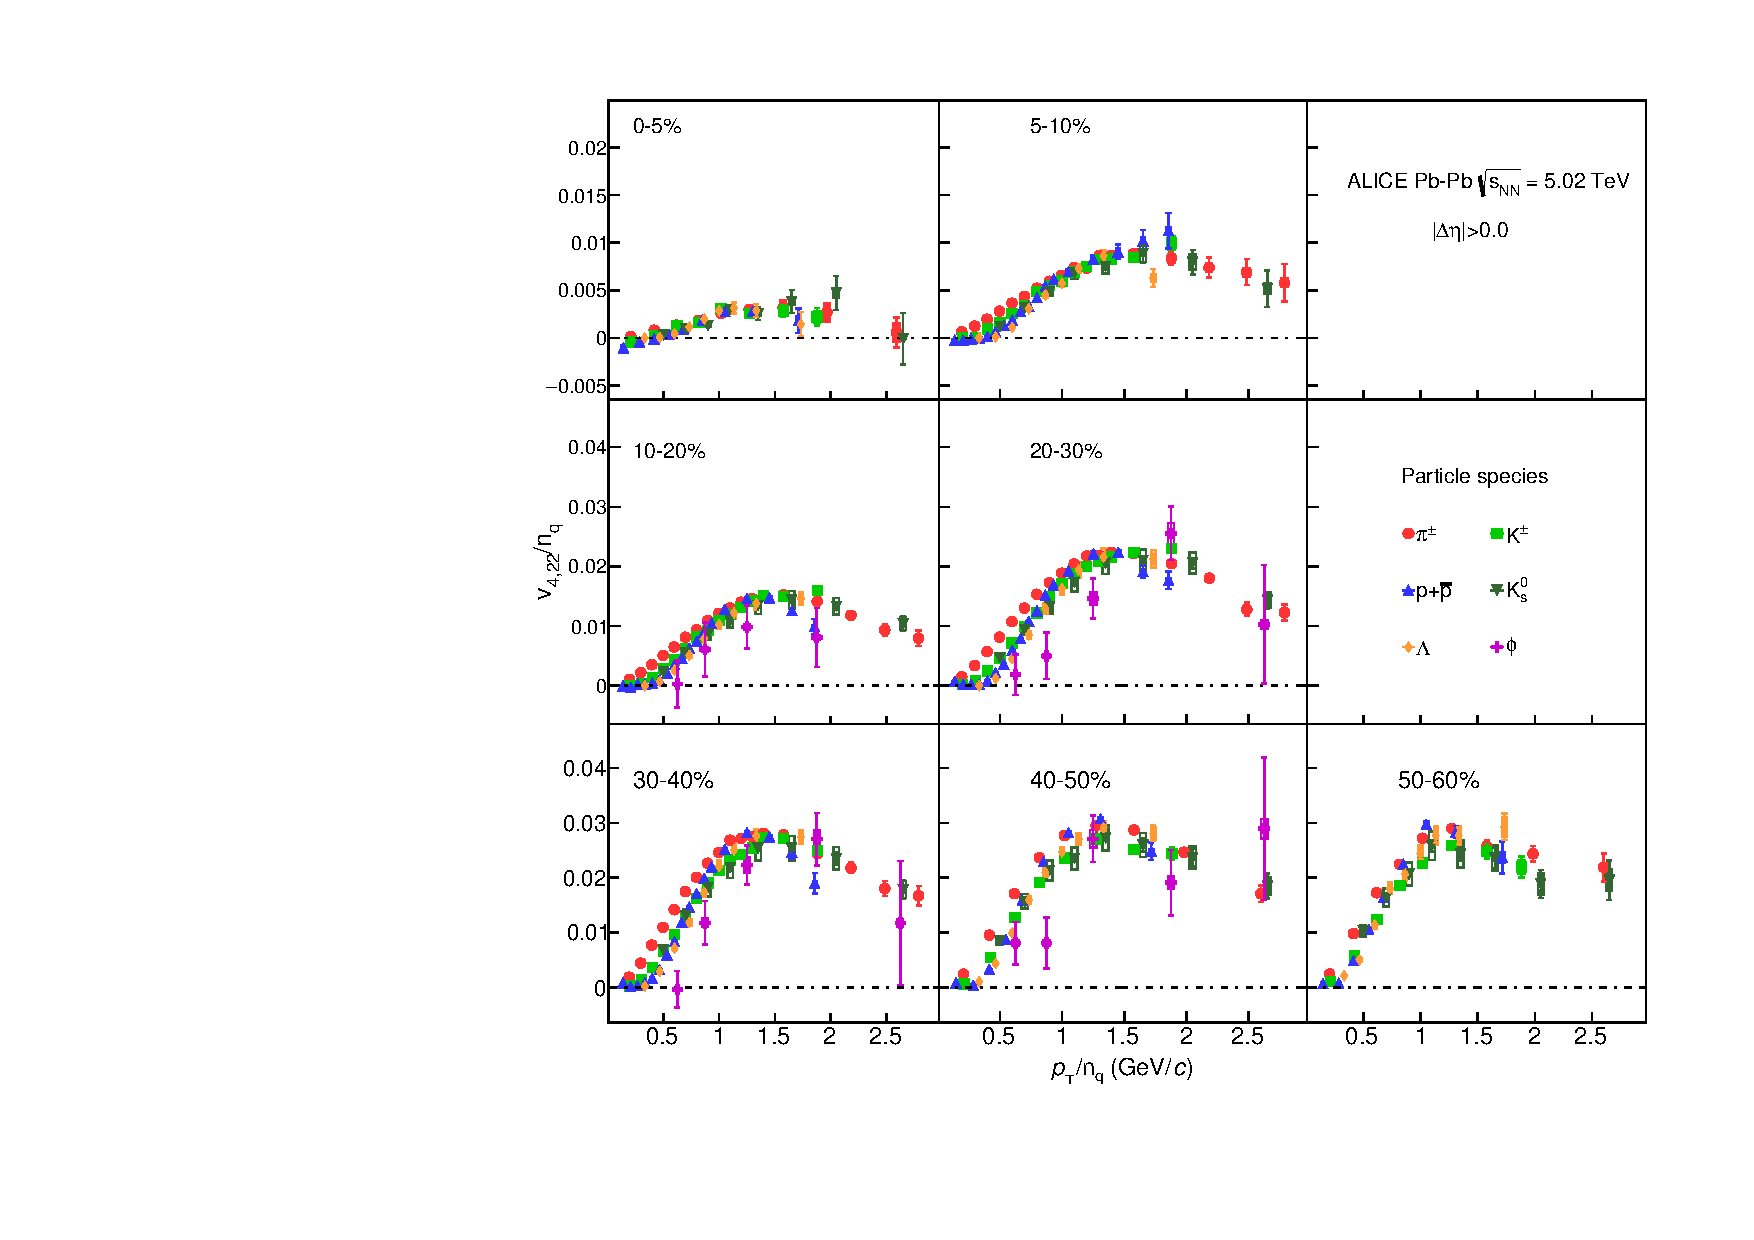
\includegraphics[scale=0.82]{figures/scaling/All_v422_gap00_NCQ_3by3.pdf}
\DIFaddendFL \end{center}
\caption{The $p_{\rm{T}}/n_{q}$-dependence of $v_{4,22}/n_{q}$ for different particle species grouped into different centrality intervals of Pb--Pb collisions \sNN}
\label{v422_NCQ}
\end{figure}

\begin{figure}[!htb]
\begin{center}
\DIFdelbeginFL %DIFDELCMD < 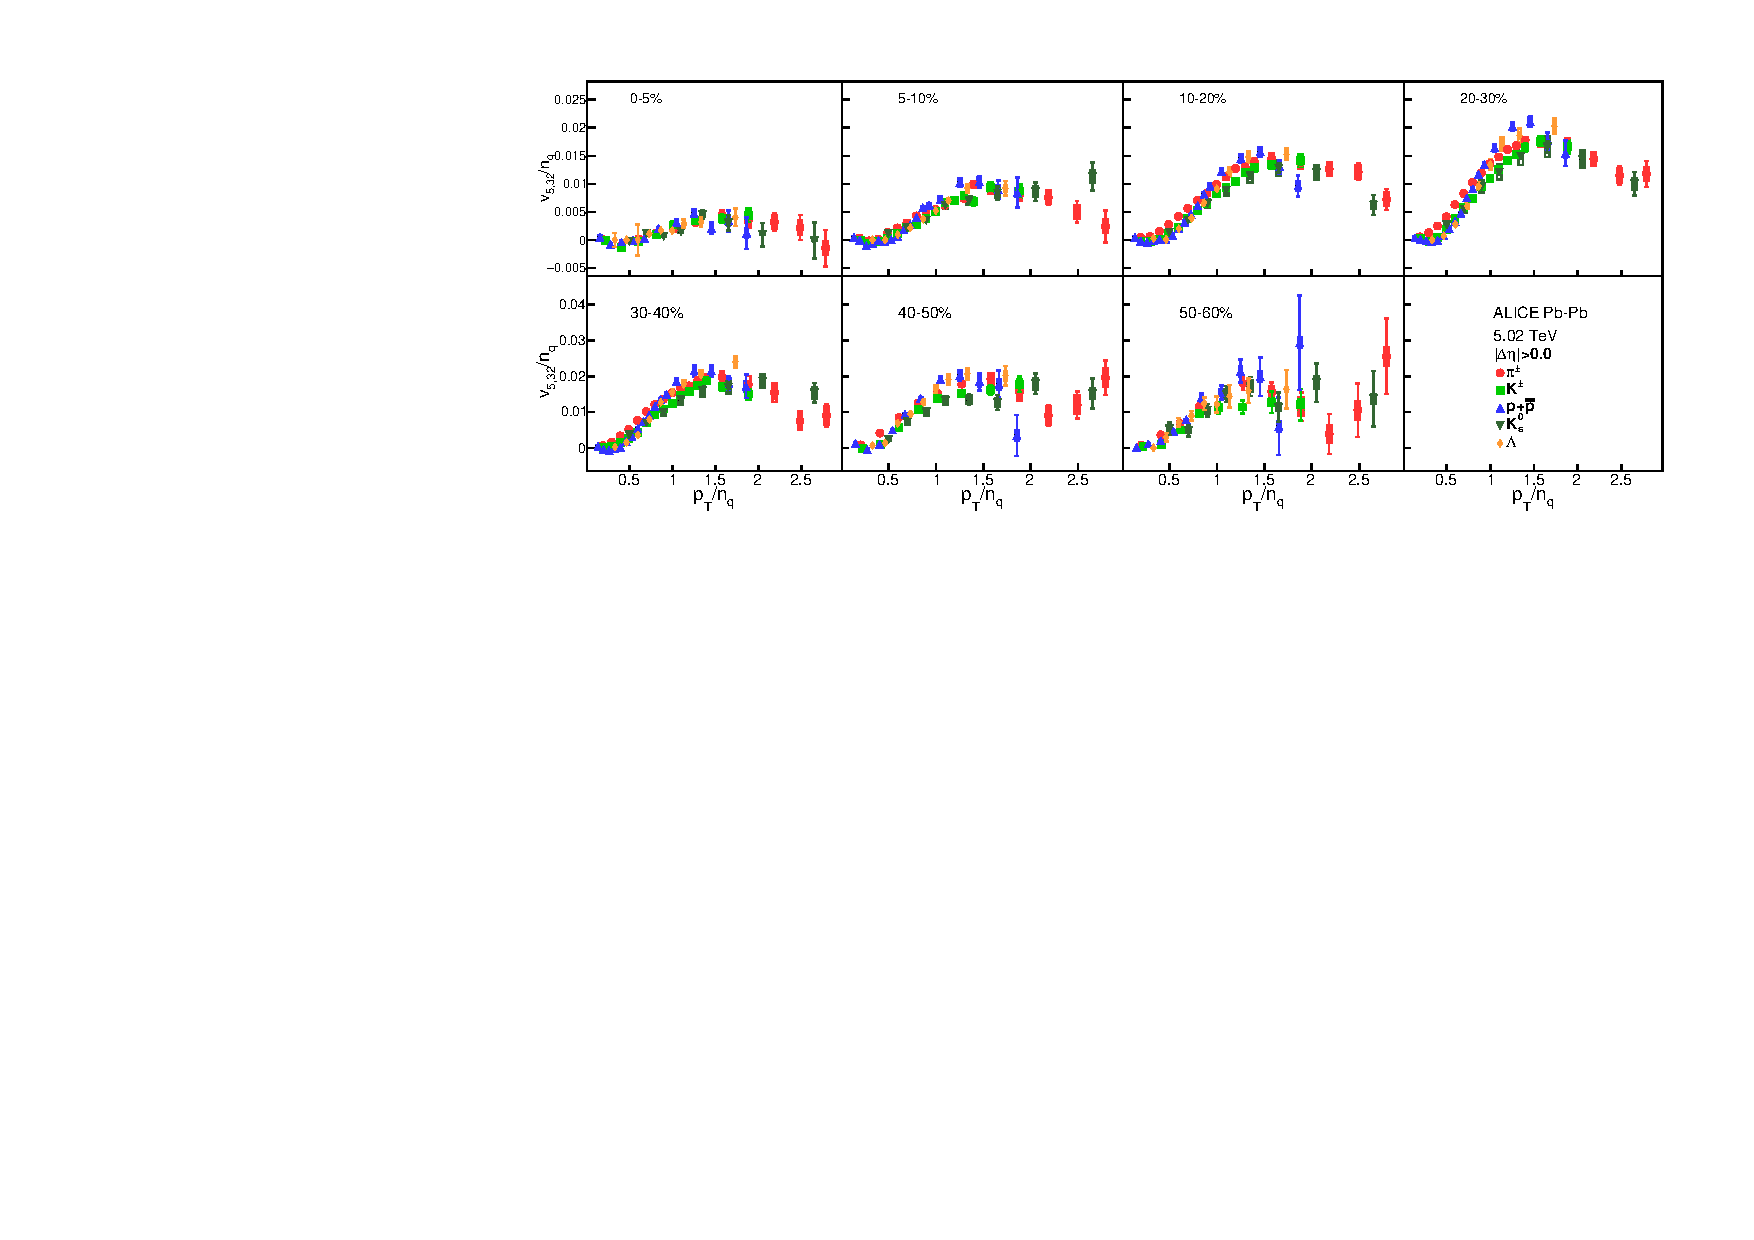
\includegraphics[scale=0.82]{figures/scaling/All_v523_gap00_NCQ.pdf}
%DIFDELCMD < %%%
\DIFdelendFL %DIF > 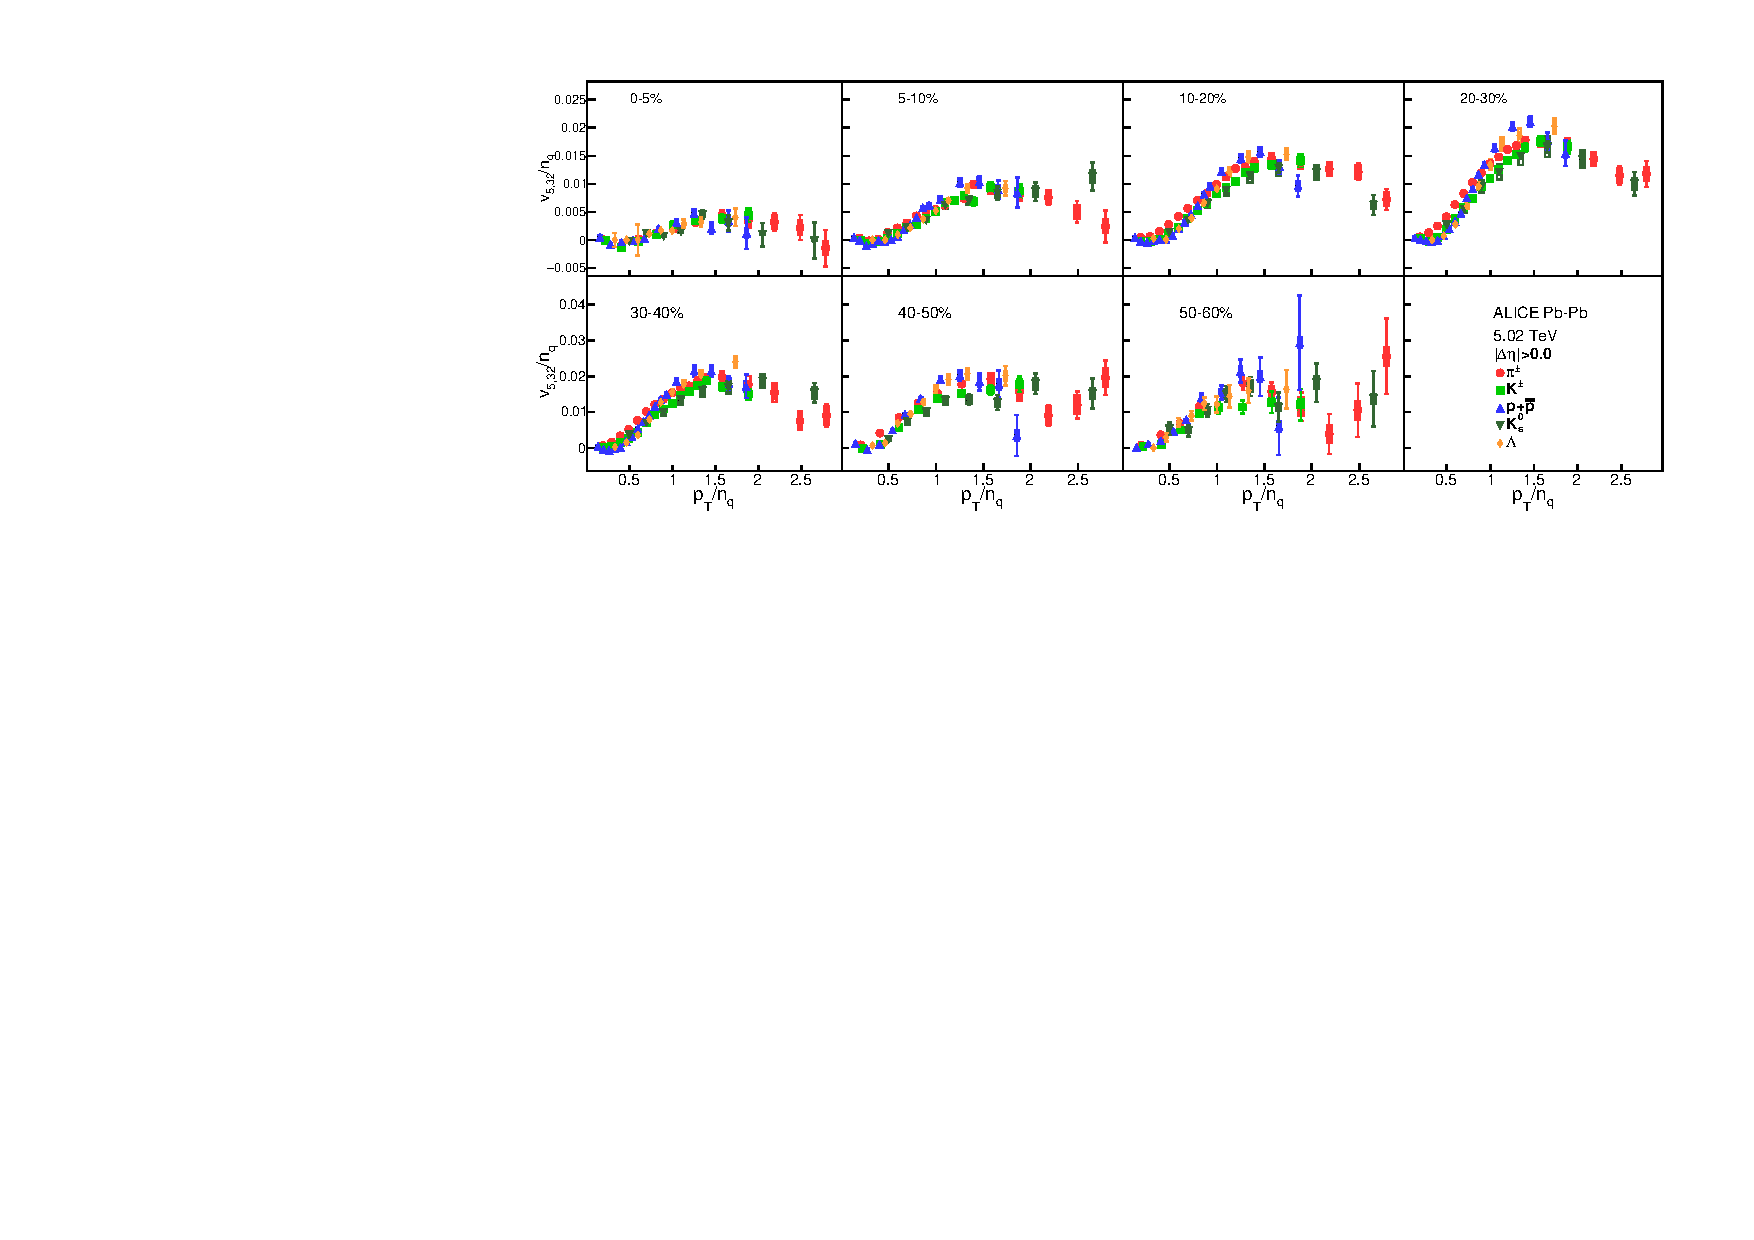
\includegraphics[scale=0.82]{figures/scaling/All_v523_gap00_NCQ.pdf}
\DIFaddbeginFL 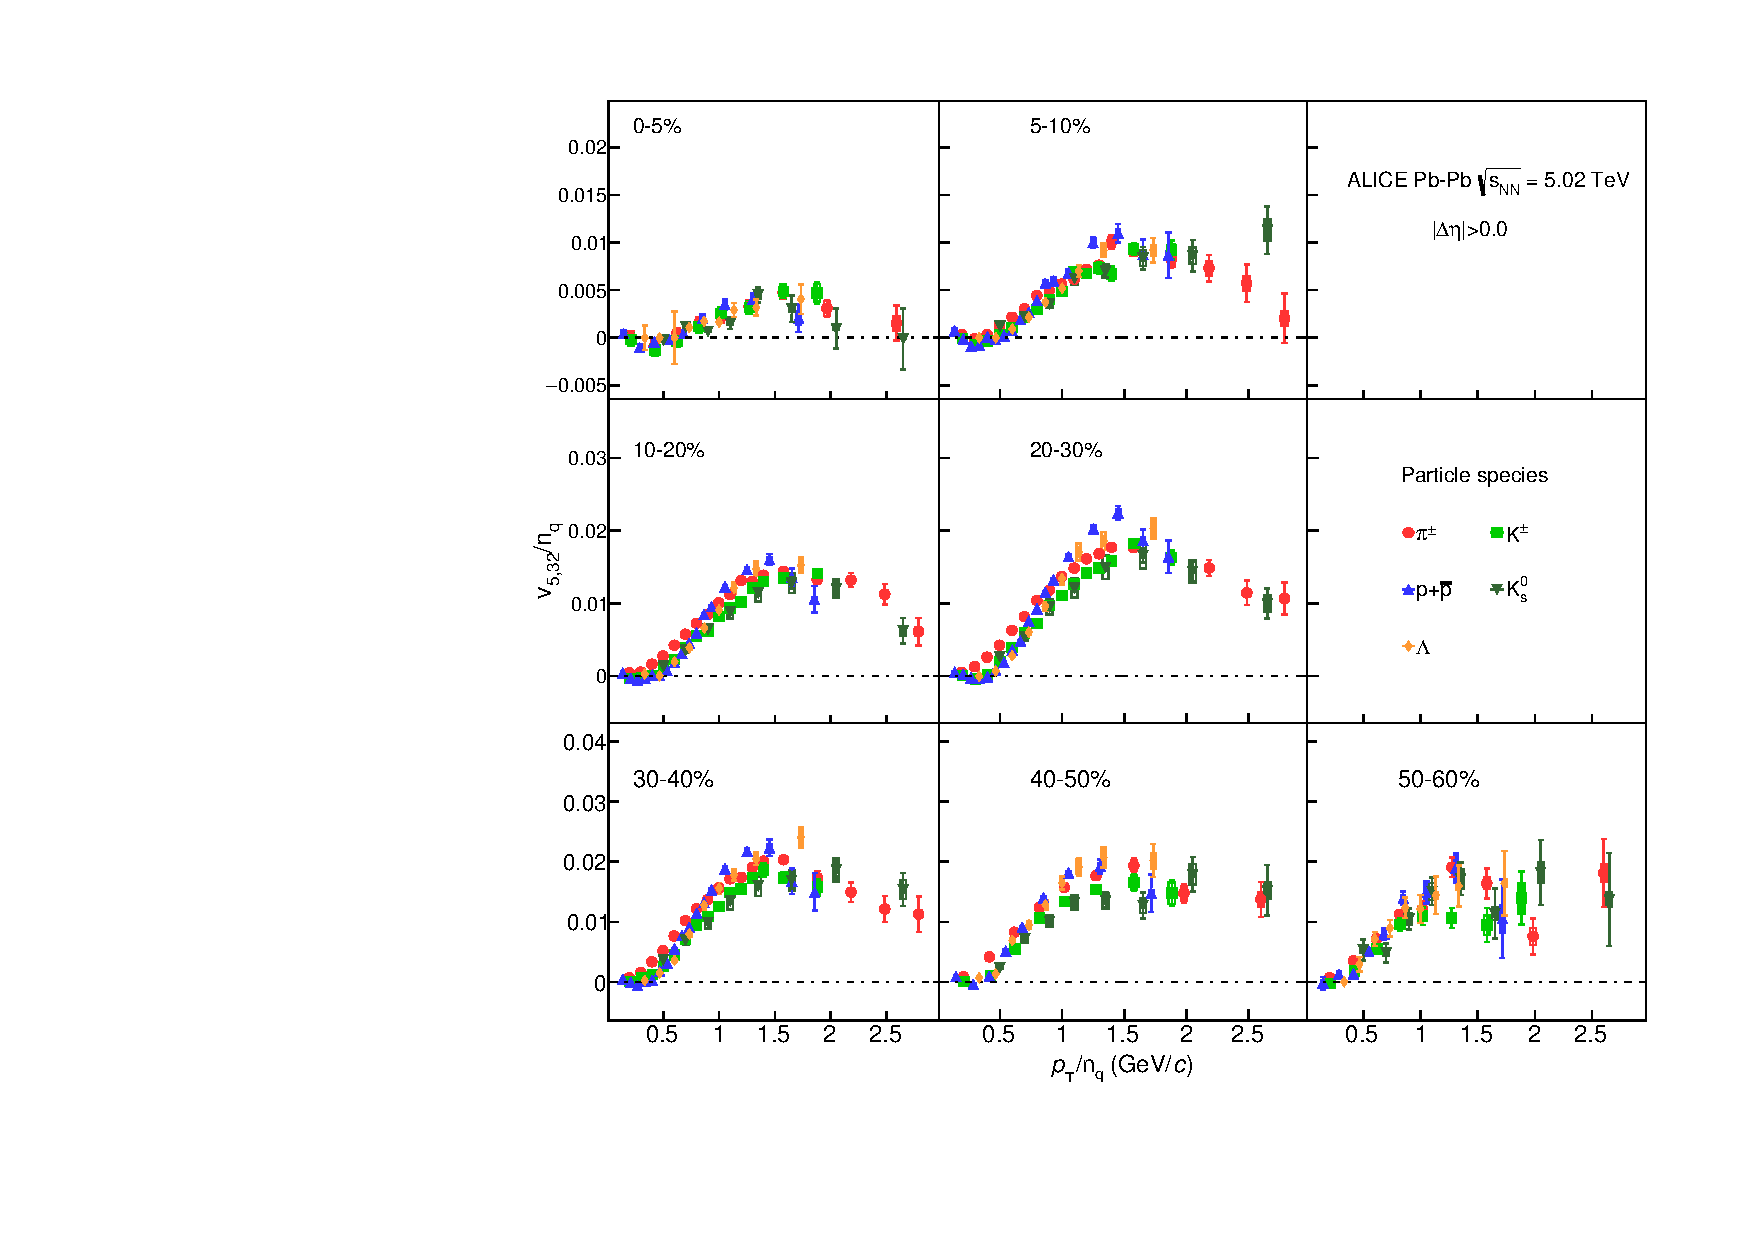
\includegraphics[scale=0.82]{figures/scaling/All_v523_gap00_NCQ_3by3.pdf}

\DIFaddendFL \end{center}
\caption{The $p_{\rm{T}}/n_{q}$-dependence of $v_{5,32}/n_{q}$ for different particle species grouped into different centrality intervals of Pb--Pb collisions \sNN}
\label{v523_NCQ}
\end{figure}

\begin{figure}[!htb]
\begin{center}
\DIFdelbeginFL %DIFDELCMD < 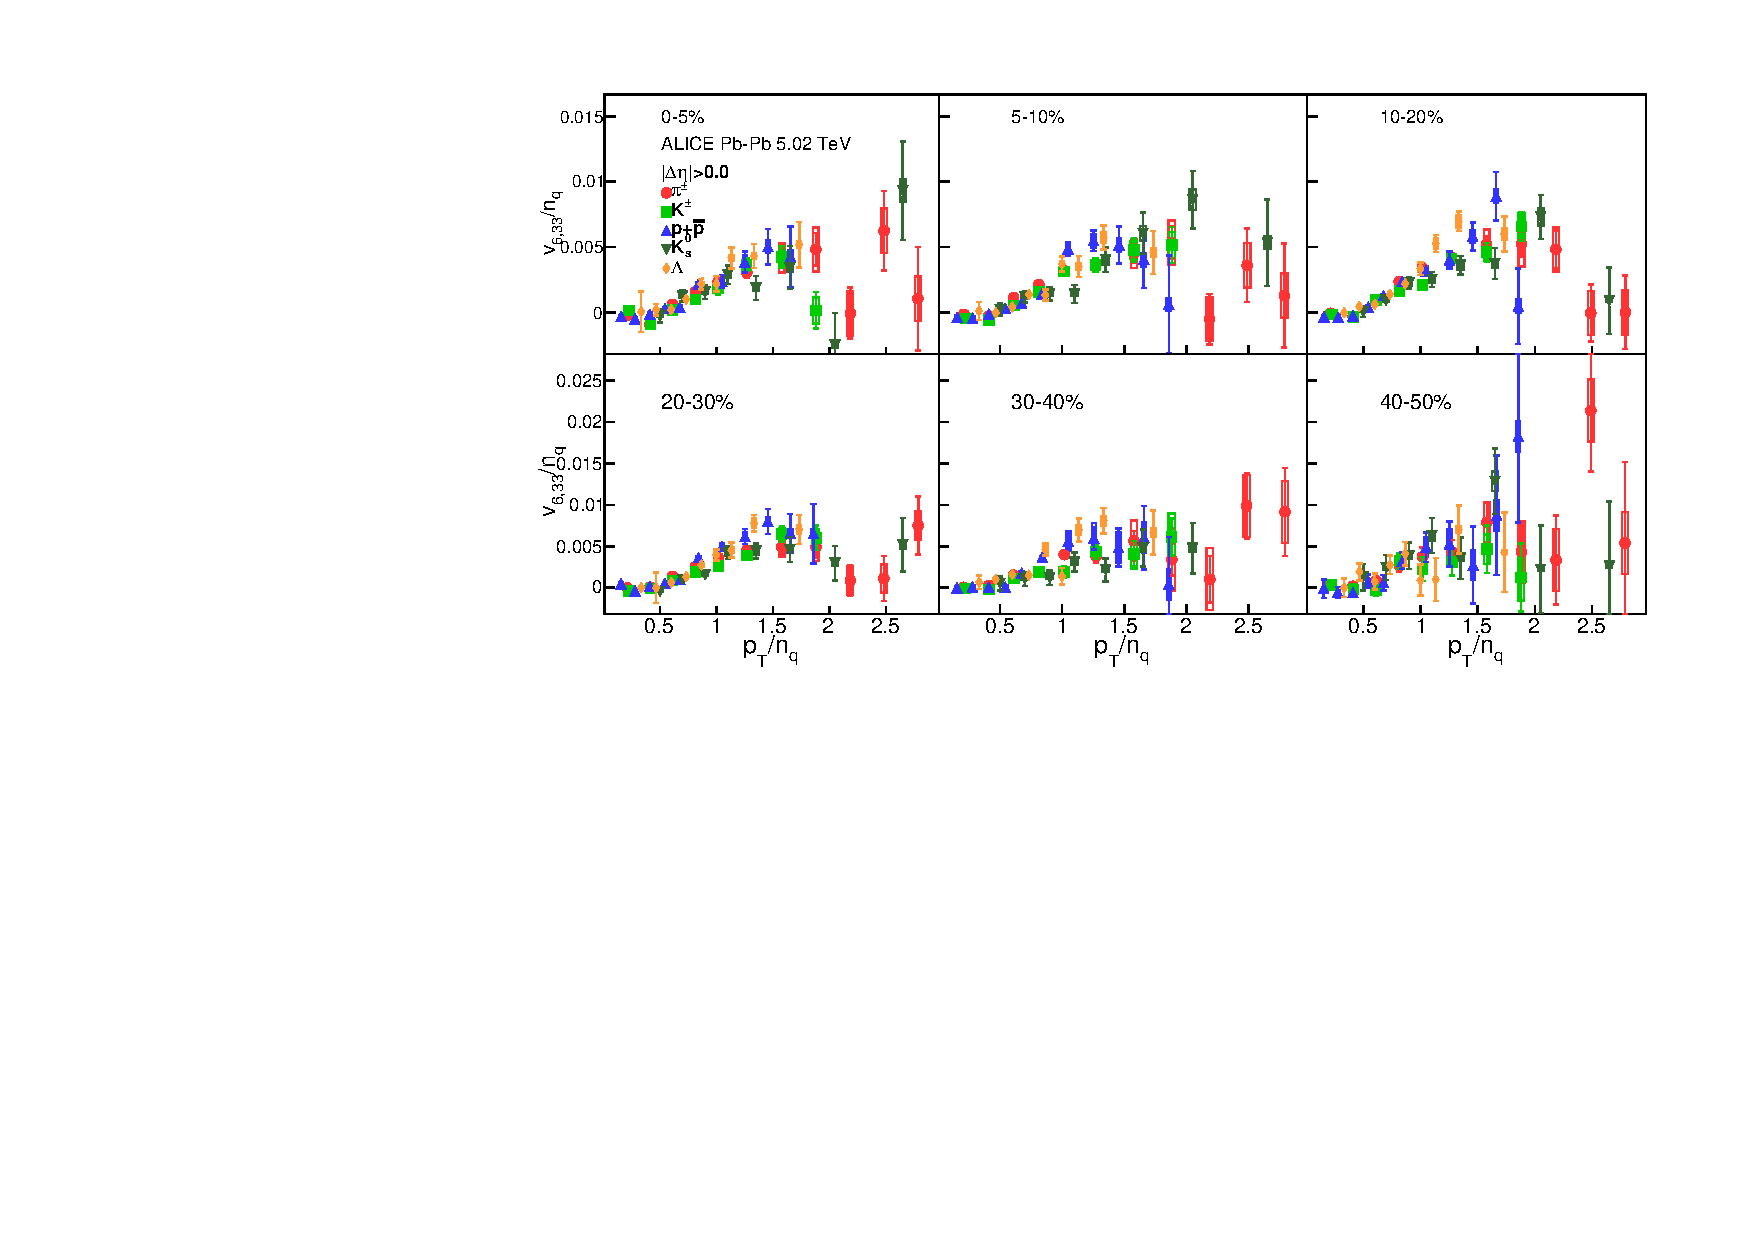
\includegraphics[scale=0.62]{figures/scaling/All_v633_gap00_NCQ.pdf}
%DIFDELCMD < %%%
\DIFdelendFL %DIF > 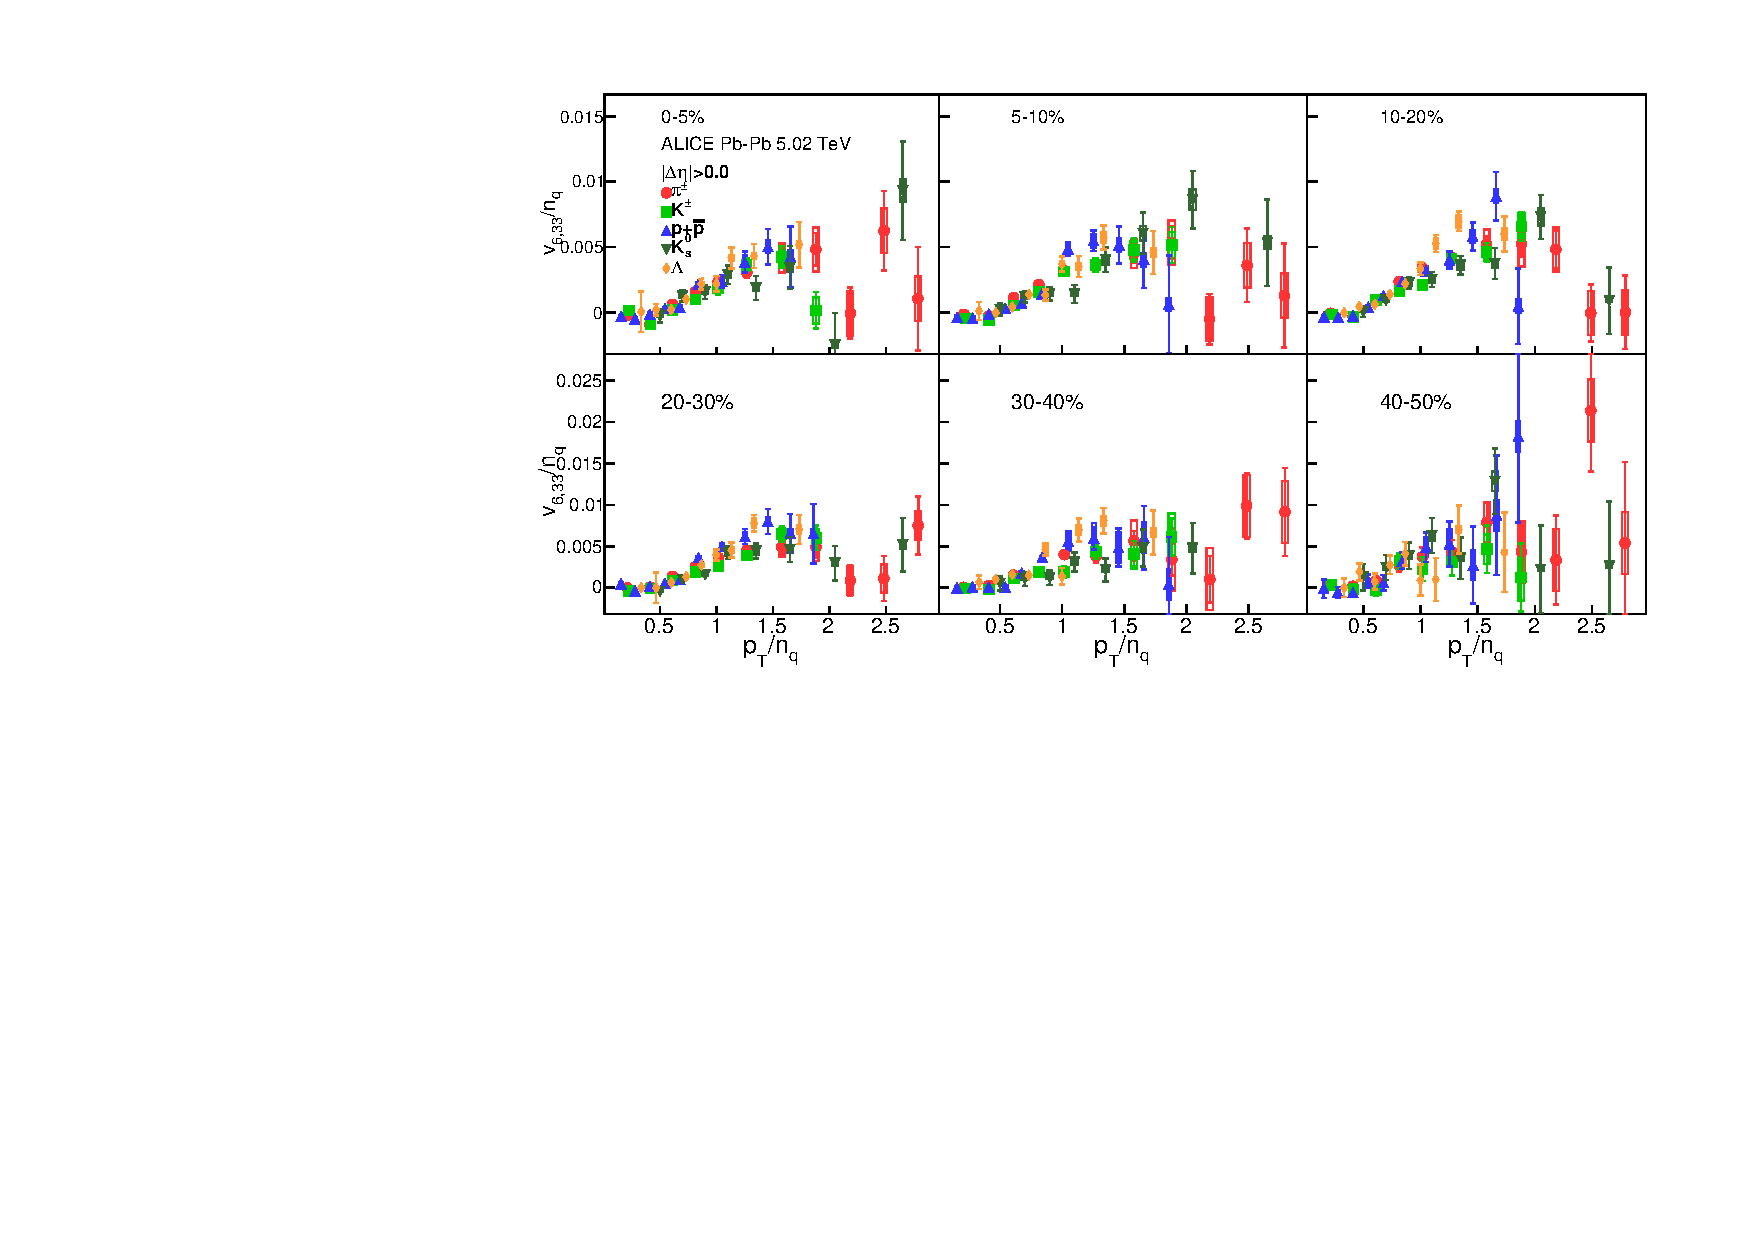
\includegraphics[scale=0.82]{figures/scaling/All_v633_gap00_NCQ.pdf}
\DIFaddbeginFL 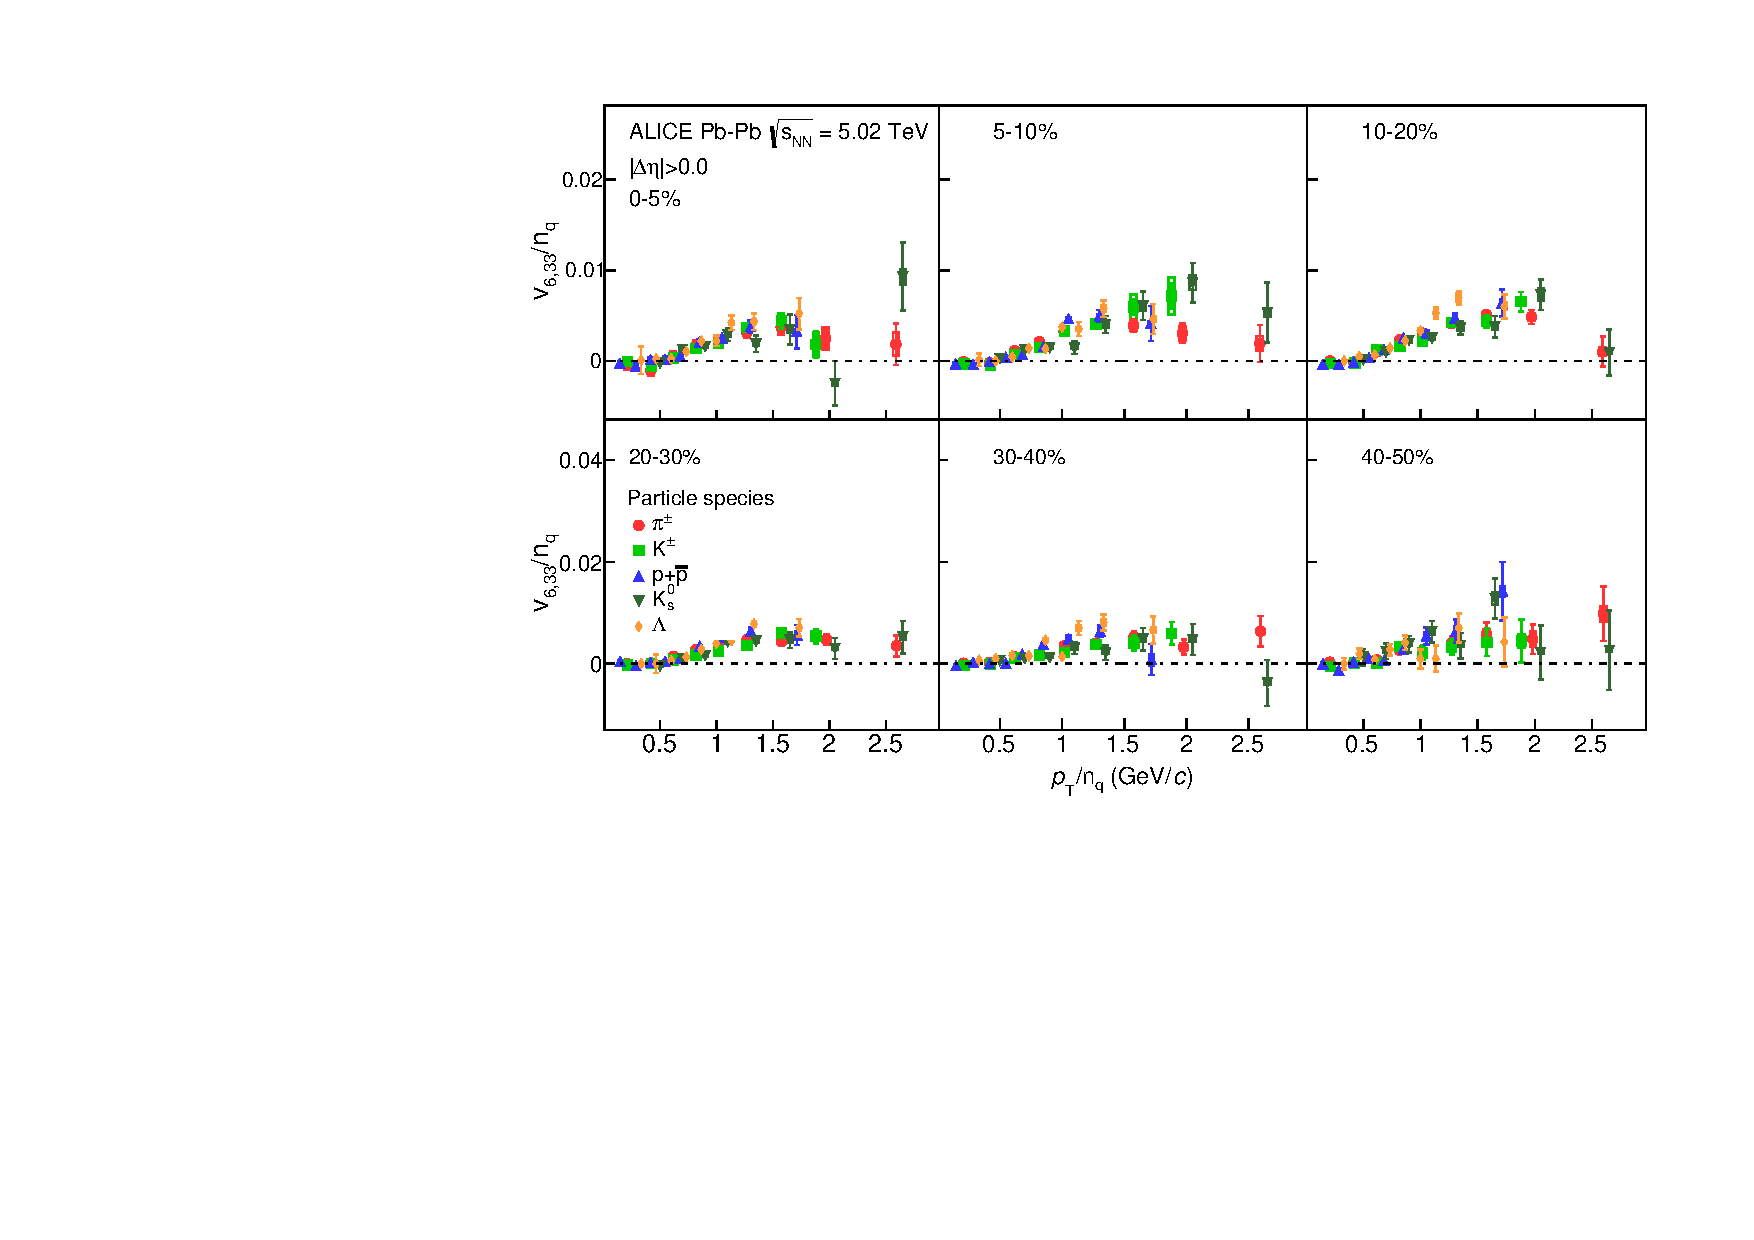
\includegraphics[scale=0.82]{figures/scaling/All_v633_gap00_NCQ_3by2.pdf}
\DIFaddendFL \end{center}
\caption{The $p_{\rm{T}}/n_{q}$-dependence of $v_{6,33}/n_{q}$ for different particle species grouped into different centrality intervals of Pb--Pb collisions \sNN}
\label{v633_NCQ}
\end{figure}

\begin{figure}[!htb]
\begin{center}
\DIFdelbeginFL %DIFDELCMD < 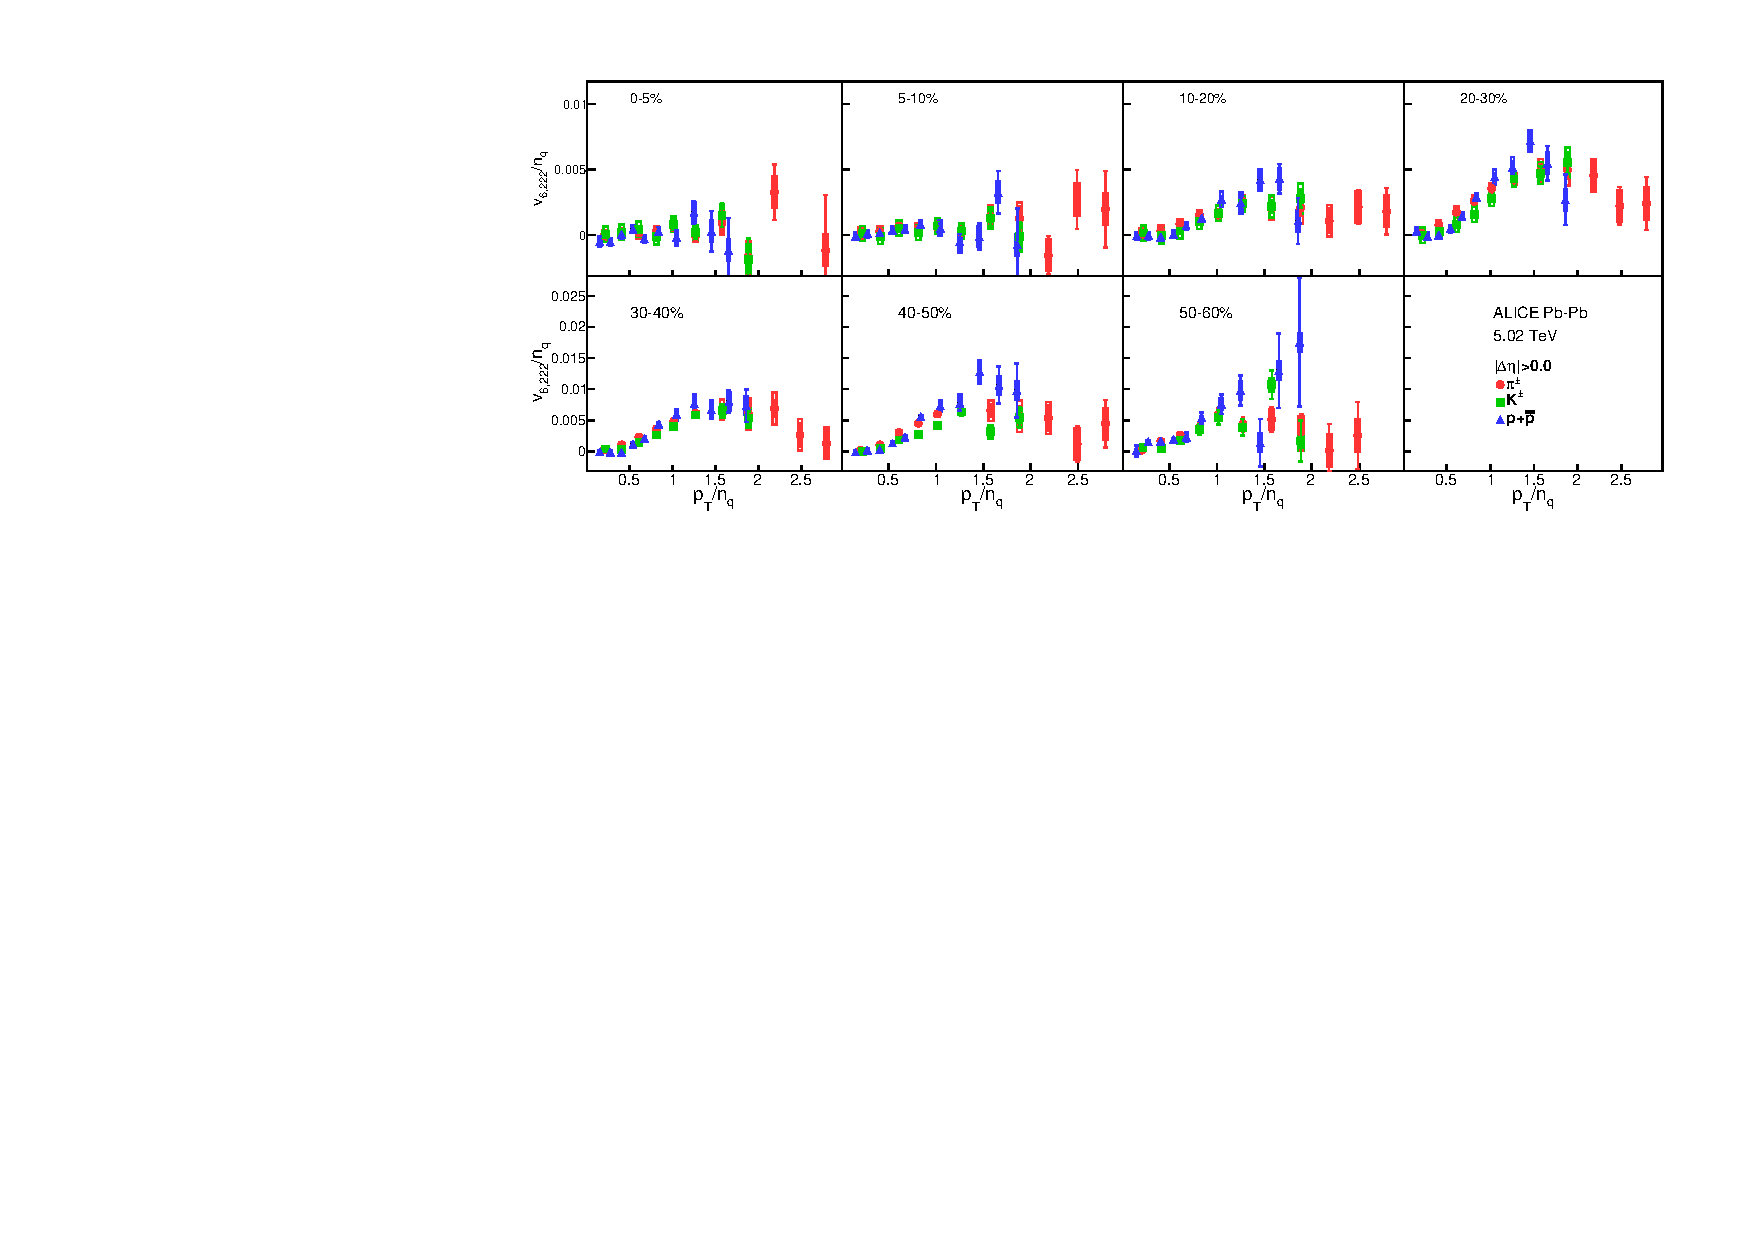
\includegraphics[scale=0.82]{figures/scaling/All_v6222_gap00_NCQ.pdf}
%DIFDELCMD < %%%
\DIFdelendFL %DIF > 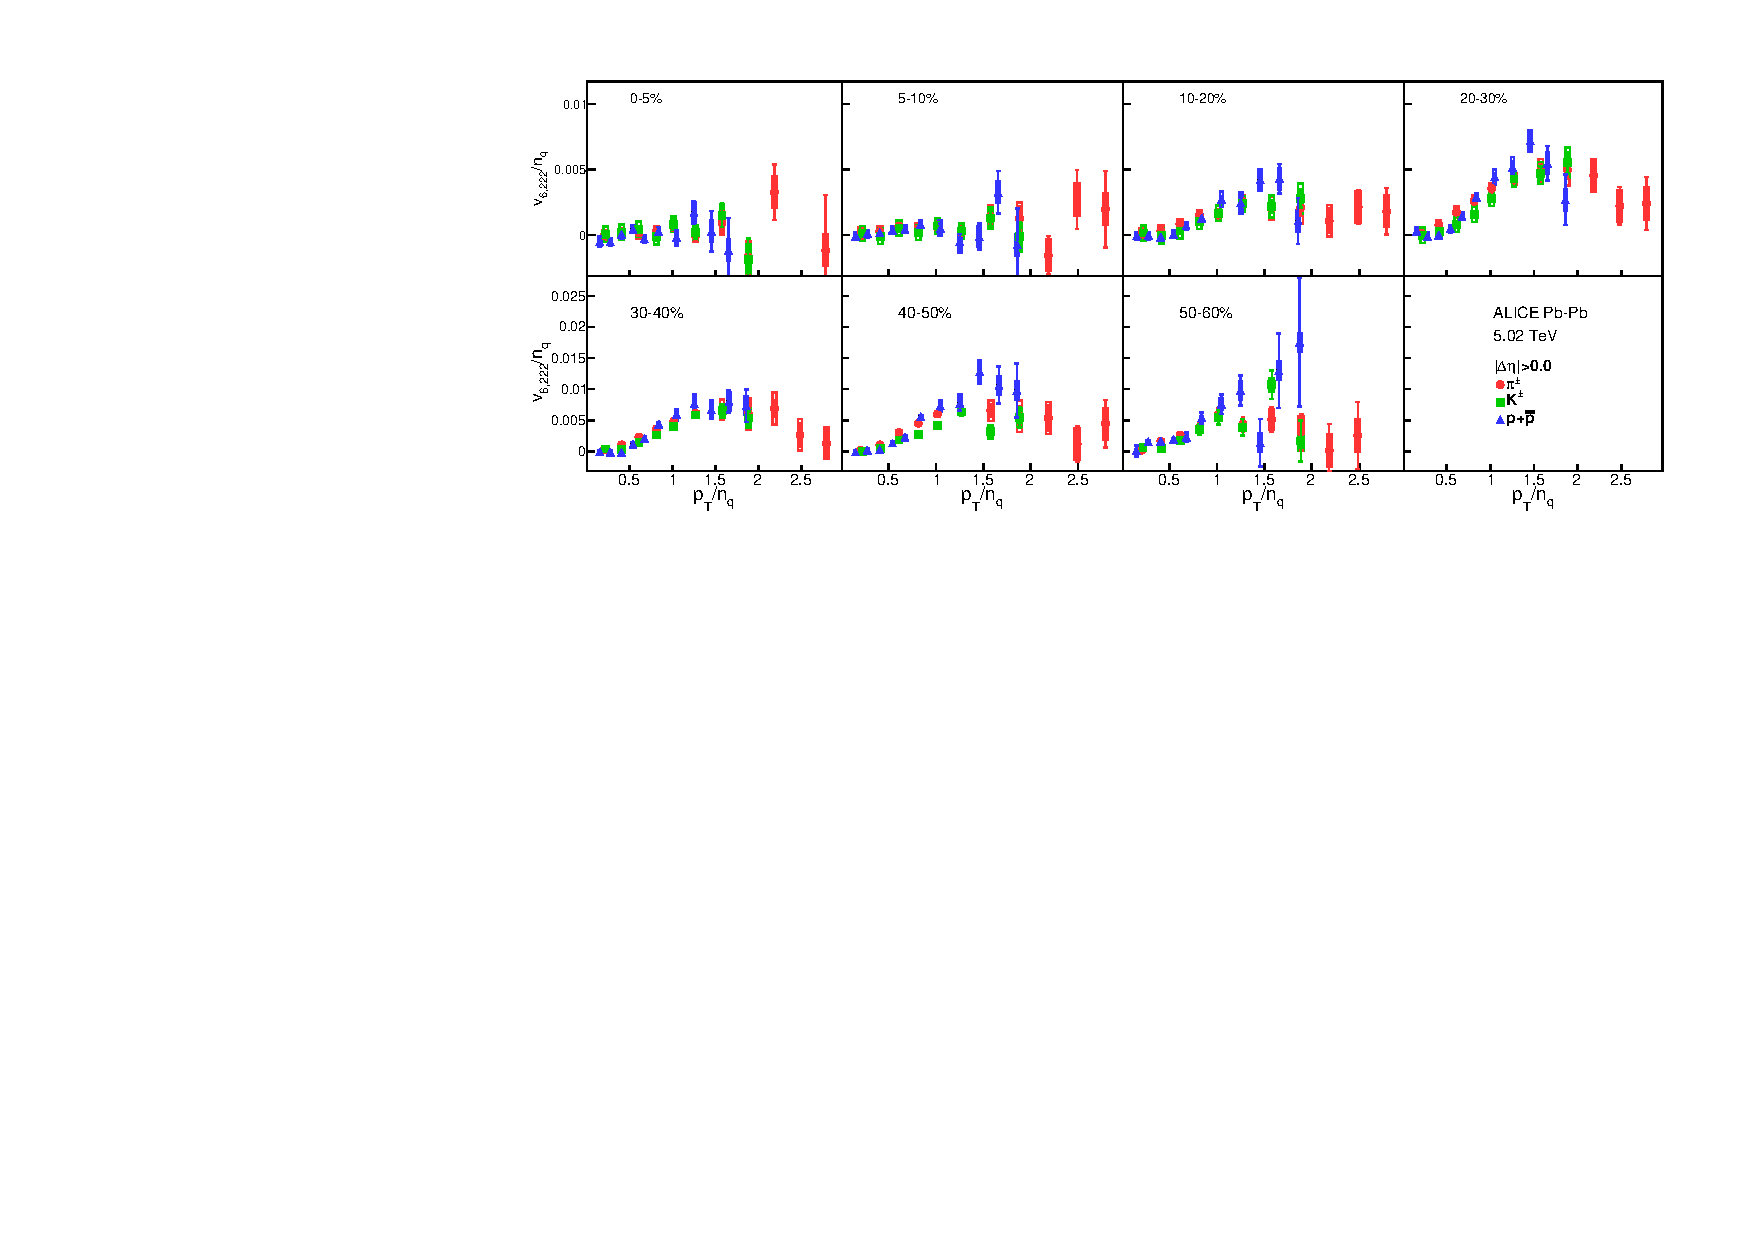
\includegraphics[scale=0.82]{figures/scaling/All_v6222_gap00_NCQ.pdf}
\DIFaddbeginFL 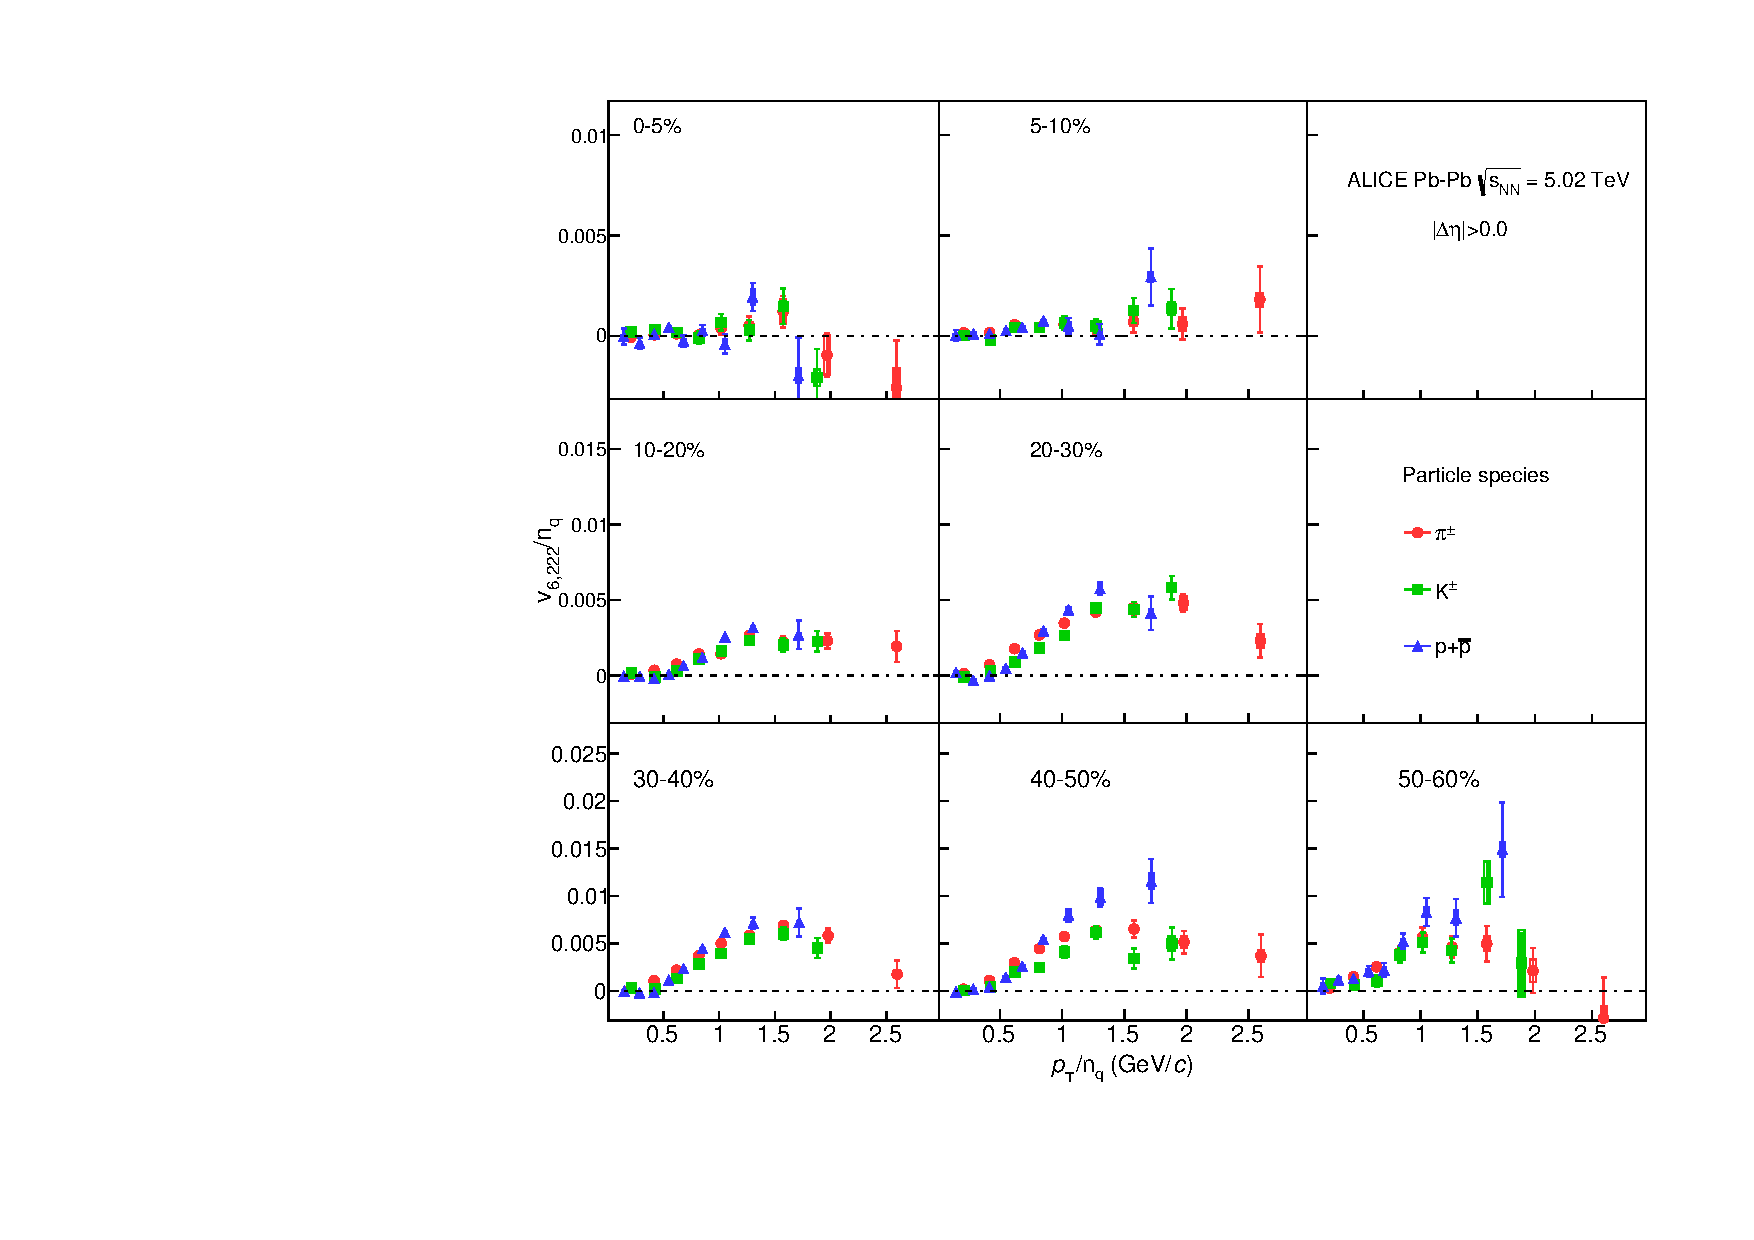
\includegraphics[scale=0.82]{figures/scaling/All_v6222_gap00_NCQ_3by3.pdf}

\DIFaddendFL \end{center}
\caption{The $p_{\rm{T}}/n_{q}$-dependence of $v_{6,222}/n_{q}$ for different particle species grouped into different centrality intervals of Pb--Pb collisions \sNN}
\label{v6222_NCQ}
\end{figure}

\newpage
\subsection{Comparison with models}
\label{SubSec:hydro}

Measurements of total flow coefficients at RHIC and LHC are described well by \DIFdelbegin \DIFdel{the }\DIFdelend hydrodynamic calculations \cite{Xu:2016hmp, McDonald:2016vlt, Zhao:2017yhj}. \DIFdelbegin \DIFdel{Recently, it was shown that the }%DIFDELCMD < \pT%%%
\DIFdel{-integrated non-linear flow modes are good observables to constrain }\DIFdelend \DIFaddbegin \DIFadd{A recent comparison between total flow measurements at ALICE \mbox{%DIFAUXCMD
\cite{Acharya:2018zuq} }%DIFAUXCMD
and two hydrodynamic calculations from \mbox{%DIFAUXCMD
\cite{Zhao:2017yhj} }%DIFAUXCMD
shed new light on }\DIFaddend the initial conditions and \DIFaddbegin \DIFadd{the }\DIFaddend transport properties of the \DIFdelbegin \DIFdel{system \mbox{%DIFAUXCMD
\cite{Acharya:2017zfg}}%DIFAUXCMD
. To further test the validity of these hydrodynamic models a comparison is performed between the measured non-linear flow modes and two hydrodynamical calculations from \mbox{%DIFAUXCMD
\cite{Zhao:2017yhj}}%DIFAUXCMD
.  }\DIFdelend \DIFaddbegin \DIFadd{created system in Pb--Pb collisions. }\DIFaddend Both calculations are based on iEBE-VISHNU \cite{Shen:2014vra}, an event-by-event version of the VISHNU hybrid model \cite{Song:2010aq} coupling $2+1$~dimensional viscous hydrodynamics (VISH2+1) \cite{Song:2007fn} to a hadronic cascade model (UrQMD). \DIFdelbegin \DIFdel{One of these models uses AMPT \mbox{%DIFAUXCMD
\cite{Lin:2004en} }%DIFAUXCMD
initial conditions with }\DIFdelend \DIFaddbegin \DIFadd{The initial conditions used for these calculations are described by AMPT \mbox{%DIFAUXCMD
\cite{Lin:2004en} }%DIFAUXCMD
and TRENTo \mbox{%DIFAUXCMD
\cite{Moreland:2014oya} }%DIFAUXCMD
both with $\tau_{0}$=0.6 fm/$c$ and $T_{sw}$ =148 MeV \mbox{%DIFAUXCMD
\cite{Bernhard:2016tnd}}%DIFAUXCMD
. These values are obtained by using Bayesian statistics from a simultaneous fit of final charged-particle density, mean transverse momentum, and integrated total flow coefficients $v_{n}$ in Pb--Pb collisions at $\sqrt{s_{\rm NN}}$ = 2.76 TeV. For  AMPT initial conditions, }\DIFaddend constant values of specific shear viscosity ($\eta/s =0.08$, the lower limit conjectured by AdS/CFT) and bulk viscosity ($\zeta/s = 0$) \DIFdelbegin \DIFdel{, and the other model incorporates }\DIFdelend \DIFaddbegin \DIFadd{are utilised, and }\DIFaddend TRENTo \cite{Moreland:2014oya} initial conditions \DIFdelbegin \DIFdel{with }\DIFdelend \DIFaddbegin \DIFadd{incorporates }\DIFaddend a temperature dependent specific shear and bulk viscosity. \DIFdelbegin \DIFdel{For simplicity in the rest of this article the model with AMPT initial conditions, $\eta/s =0.08$ and $\zeta/s =0$ is referred to as AMPT and the model with TRENTo initial conditions}\DIFdelend \DIFaddbegin \footnote{ \DIFadd{For simplicity in the rest of this article the model with AMPT initial conditions, $\eta/s =0.08$ and $\zeta/s =0$ is referred to as AMPT and the model with TRENTo initial conditions, $\eta/s(\rm{T})$ and $\zeta/s(\rm{T})$ is referred to as TRENTo.}} \DIFadd{The comparison between the total flow measurements and these two calculations illustrates a qualitative agreement. This agreement between the data and the models depends on the particle species, transverse momentum range and centrality percentile and overall the AMPT model reproduces these measurements more accurately than TRENTo \mbox{%DIFAUXCMD
\cite{Acharya:2018zuq}}%DIFAUXCMD
.
}

\DIFadd{Recently, it was shown that the }\pT\DIFadd{-integrated non-linear flow modes are good observables to constrain the initial conditions and transport properties of the system \mbox{%DIFAUXCMD
\cite{Acharya:2017zfg}}%DIFAUXCMD
. To further constrain the initial conditions and transport properties of the system and test the validity of these hydrodynamic models a comparison is performed between the measured }\pT\DIFadd{-dependent non-linear flow modes for }\pion\DIFaddend , \DIFdelbegin \DIFdel{$\eta/s(\rm{T})$ and $\zeta/s(\rm{T})$ is referred to as TRENTo}\DIFdelend \DIFaddbegin \kaon\DIFadd{~and }\proton\DIFadd{~with two hydrodynamical calculations from \mbox{%DIFAUXCMD
\cite{Zhao:2017yhj} }%DIFAUXCMD
as were used in comparison to the total flow measurements \mbox{%DIFAUXCMD
\cite{Acharya:2018zuq}}%DIFAUXCMD
}\DIFaddend . 


%DIF > To test the validity of these hydrodynamic models a comparison is performed between the measured non-linear flow modes and two hydrodynamical calculations from \cite{Zhao:2017yhj}.  Both calculations are based on iEBE-VISHNU \cite{Shen:2014vra}, an event-by-event version of the VISHNU hybrid model \cite{Song:2010aq} coupling $2+1$~dimensional viscous hydrodynamics (VISH2+1) \cite{Song:2007fn} to a hadronic cascade model (UrQMD). One of these models uses AMPT \cite{Lin:2004en} initial conditions with constant values of specific shear viscosity ($\eta/s =0.08$, the lower limit conjectured by AdS/CFT) and bulk viscosity ($\zeta/s = 0$), and the other model incorporates TRENTo \cite{Moreland:2014oya} initial conditions with a temperature dependent specific shear and bulk viscosity. 
\DIFaddbegin 

%DIF > Both calculations are based on iEBE-VISHNU \cite{Shen:2014vra}, an event-by-event version of the VISHNU hybrid model \cite{Song:2010aq} coupling $2+1$~dimensional viscous hydrodynamics (VISH2+1) \cite{Song:2007fn} to a hadronic cascade model (UrQMD). One of these models uses AMPT \cite{Lin:2004en} initial conditions with constant values of specific shear viscosity ($\eta/s =0.08$, the lower limit conjectured by AdS/CFT) and bulk viscosity ($\zeta/s = 0$), and the other model incorporates TRENTo \cite{Moreland:2014oya} initial conditions with a temperature dependent specific shear and bulk viscosity. 

\DIFaddend Figures \ref{v422_model}, \ref{v523_model}, \ref{v633_model} and \ref{v6222_model} present the comparison between the measurements (data points in the plots) and both models for the \pT-differential $v_{4,22}$, $v_{5,32}$, $v_{6,33}$ and $v_{6,222}$, respectively, for \pion, \kaon~and \proton~at 0-10\% up to 50-60\% centrality interval (40-50\% centrality interval for $v_{6,33}$) of Pb--Pb collisions at \sNN. The solid bands show the AMPT model and the hatched bands represent the TRENTo calculations. The bottom panels in each plot in Figs. \ref{v422_model}, \ref{v523_model}, \ref{v633_model} and \ref{v6222_model} present the difference between the models and the measurement. Both models produce a mass ordering in $p_{\rm{T}}<2.5$ \GeV. The comparison between the models and the the measurements of $v_{4,22}$ reveals that in more central collisions they reproduce the data however as centrality decreases the models start to deviate from the data. This pattern repeats for $v_{5,32}$ in which AMPT reproduces the data relatively better. The comparison between the measurements and the models  for $v_{6,222}$ and $v_{6,33}$ shows that the models are able to reproduce the data only up to 30-40\% and 20-30\% centrality intervals, respectively. 


%The comparisons show slightly better agreement between the data and the model which uses AMPT as the initial conditions but both models need to be tuned to data further to describe these sensitive flow modes.

 \begin{figure}[!htb]
\begin{center}
\DIFdelbeginFL %DIFDELCMD < 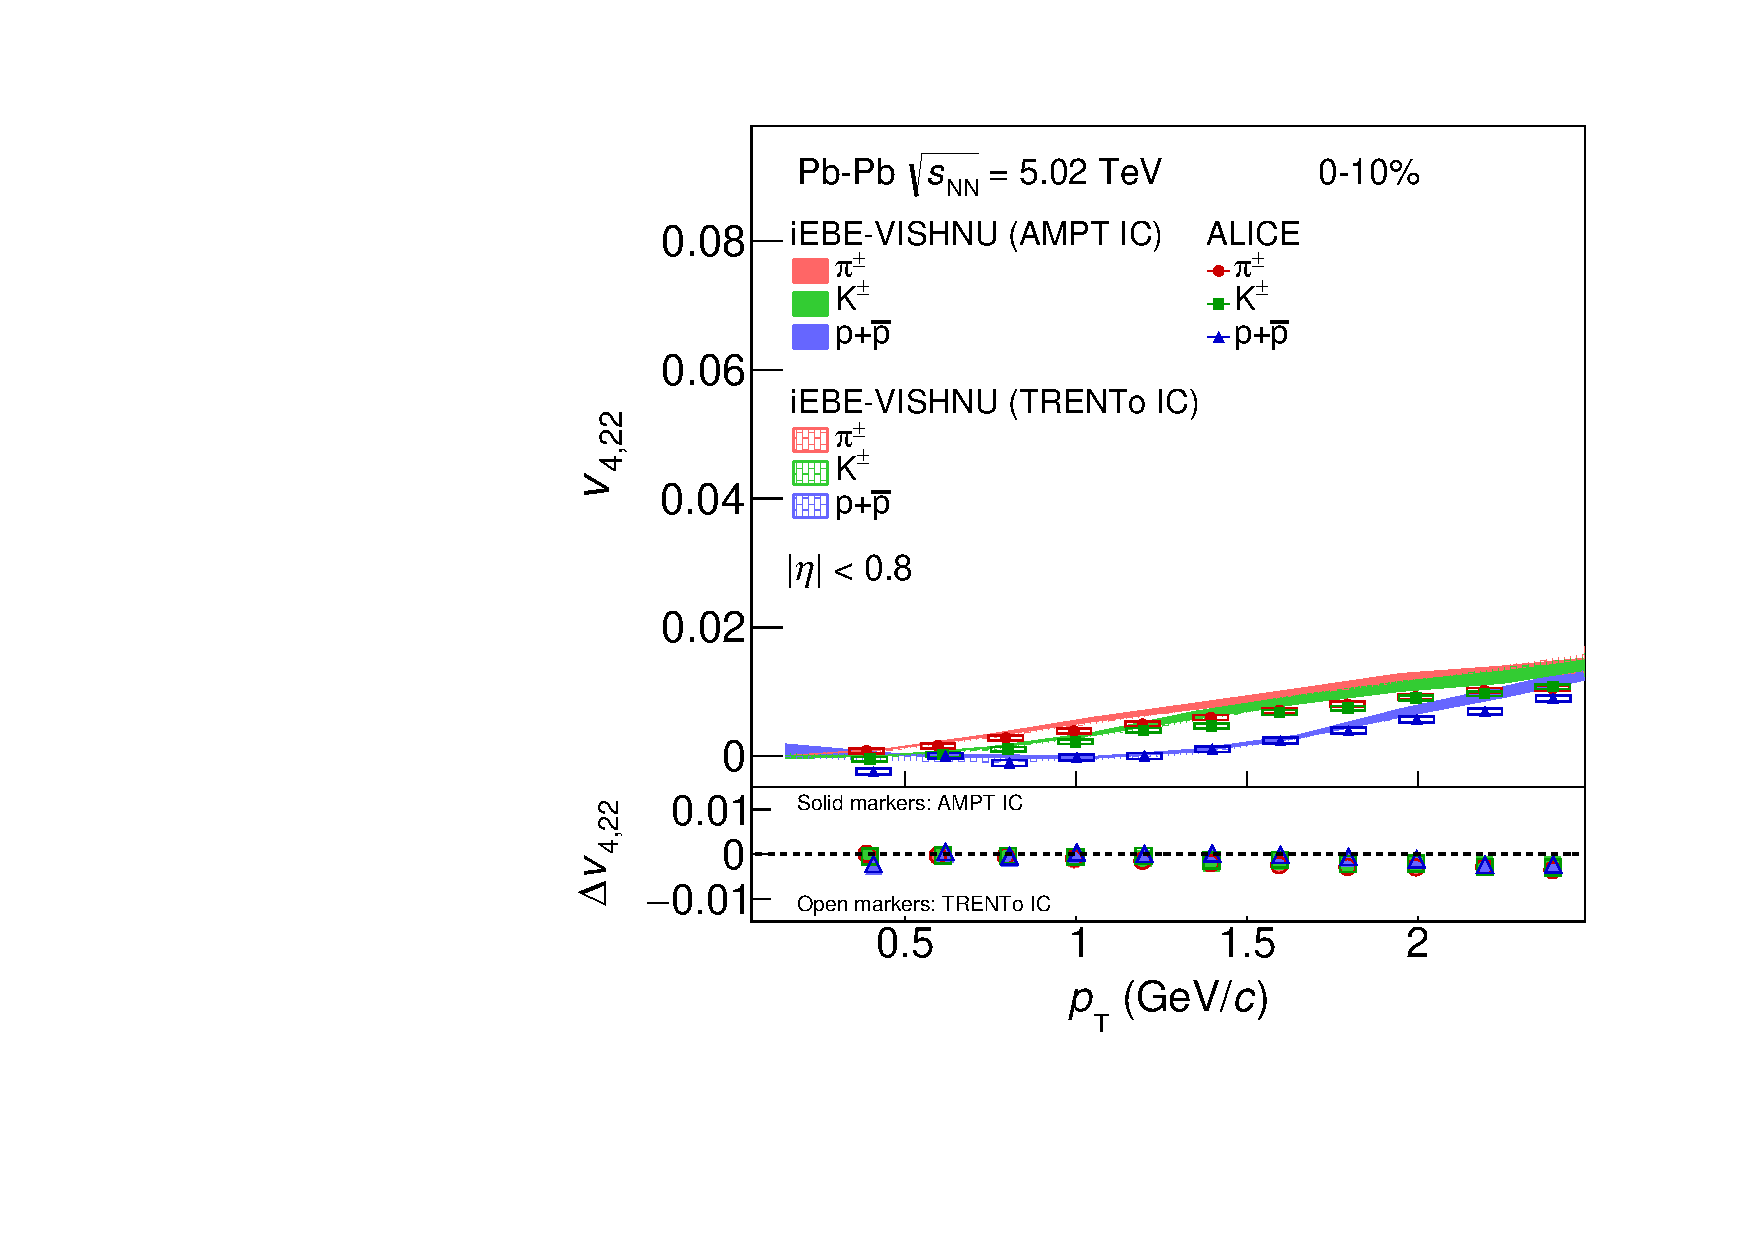
\includegraphics[scale=0.26]{figures/model/TrentoAndAMPT_v422_gap00_new_0-10_PID2.pdf}
%DIFDELCMD < 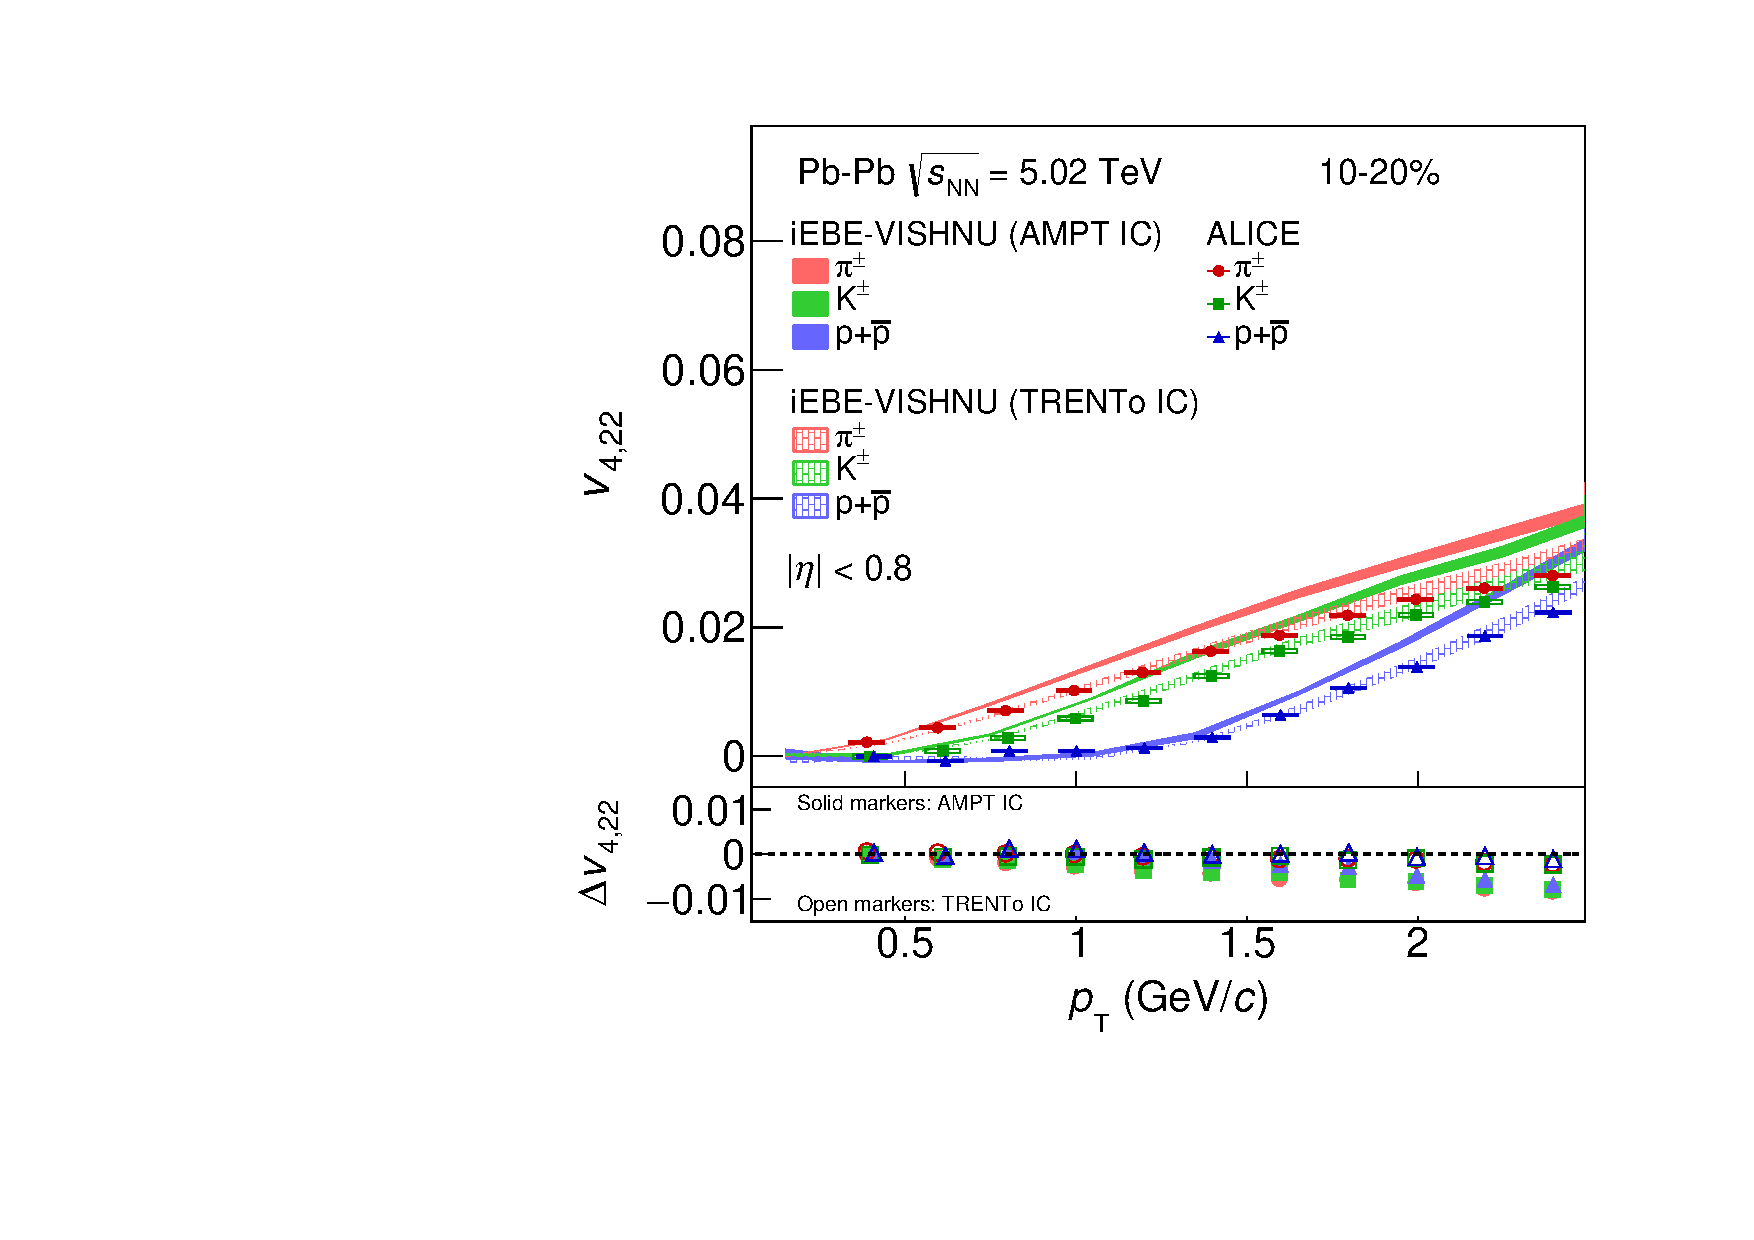
\includegraphics[scale=0.26]{figures/model/TrentoAndAMPT_v422_gap00_new_10-20_PID2.pdf}
%DIFDELCMD < 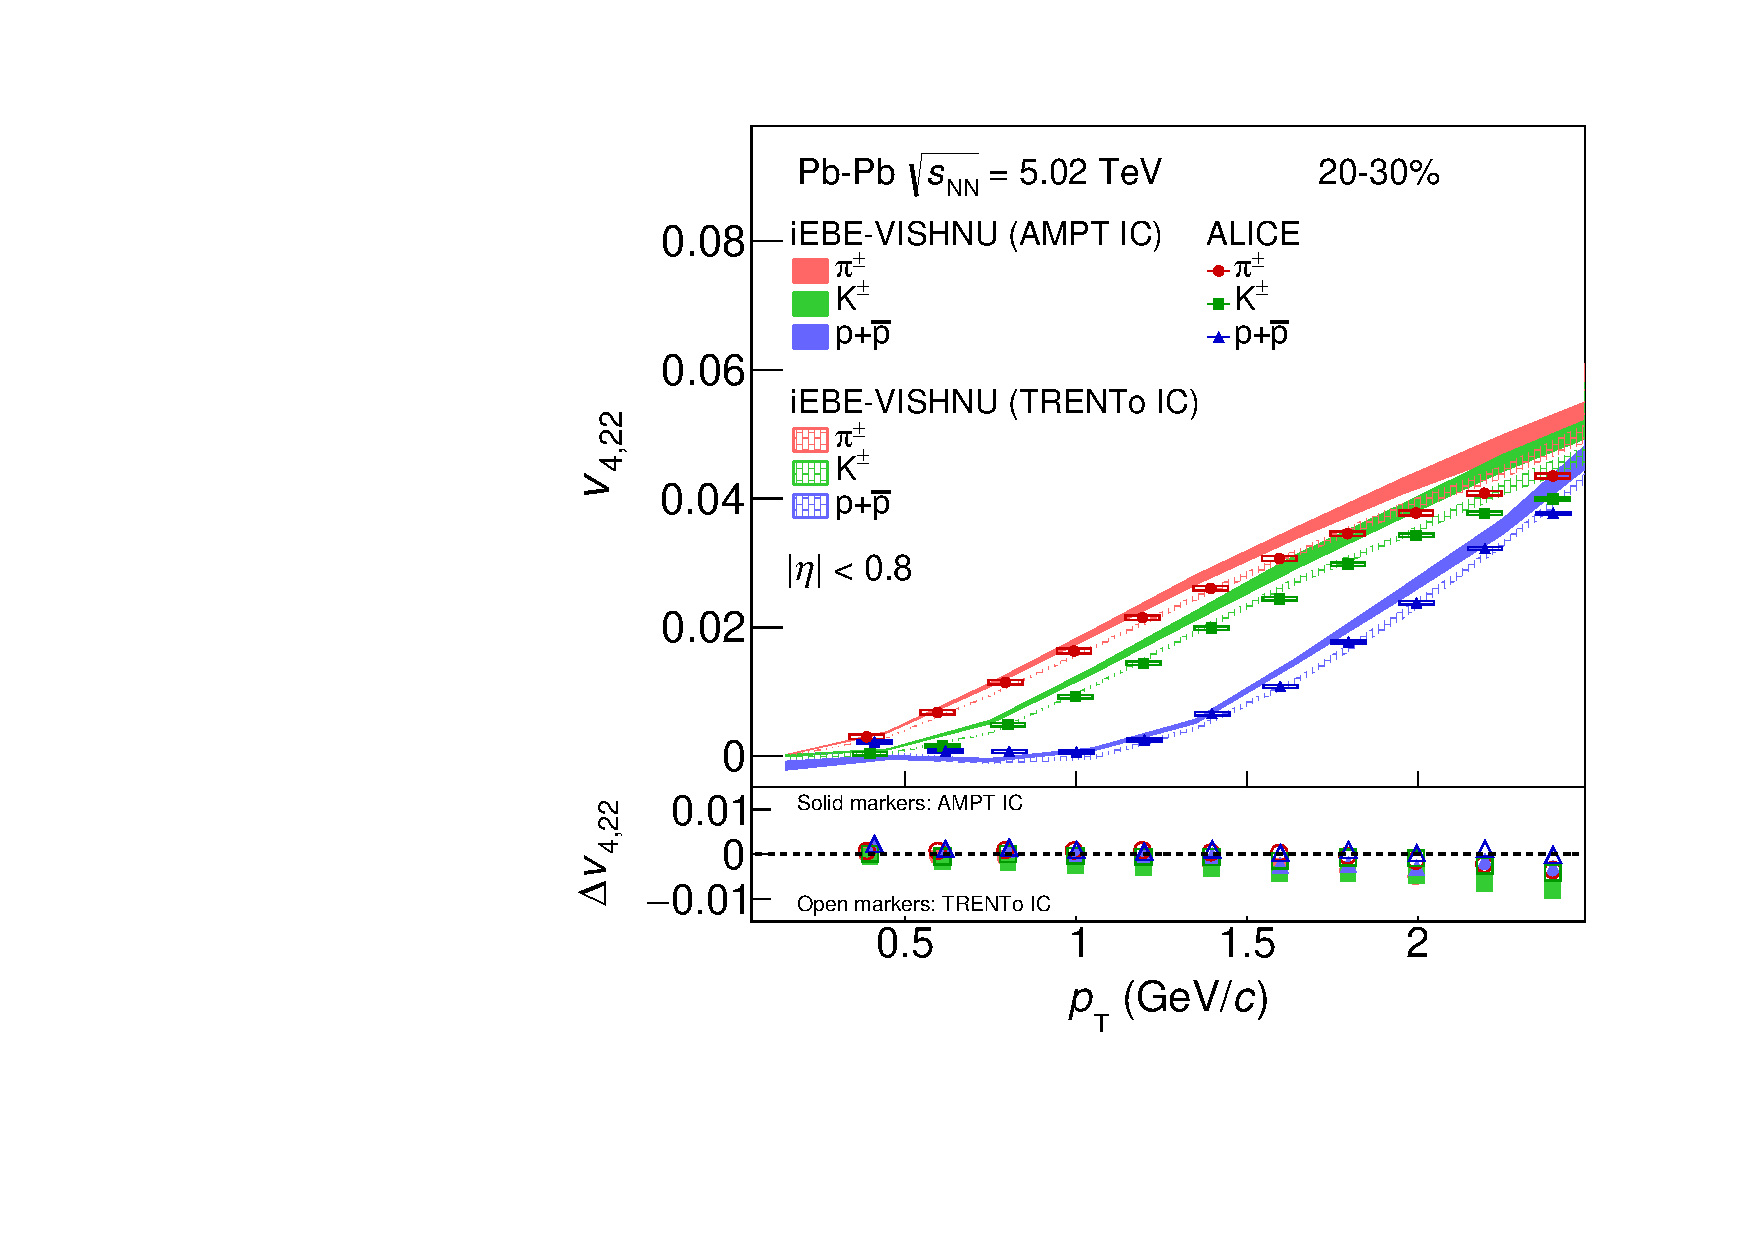
\includegraphics[scale=0.26]{figures/model/TrentoAndAMPT_v422_gap00_new_20-30_PID2.pdf}
%DIFDELCMD < 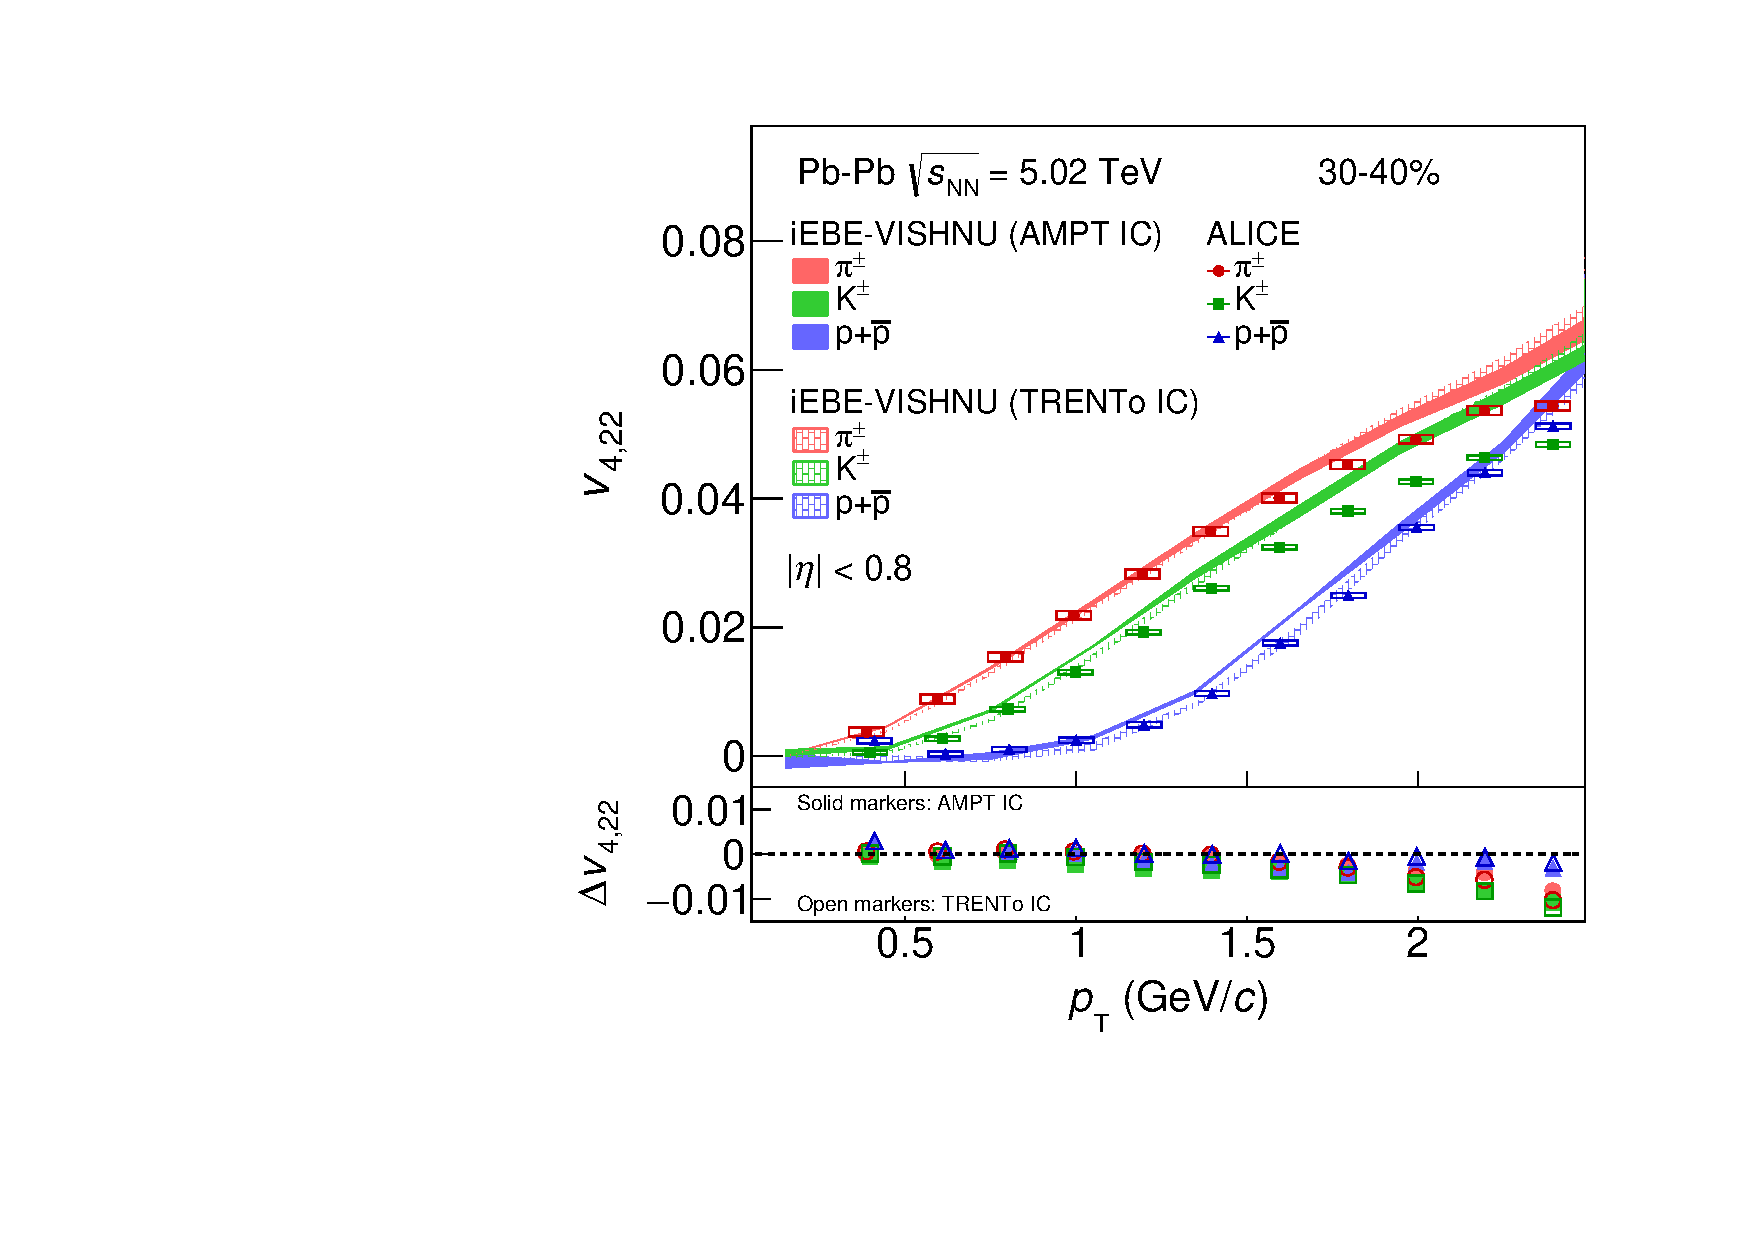
\includegraphics[scale=0.26]{figures/model/TrentoAndAMPT_v422_gap00_new_30-40_PID2.pdf}
%DIFDELCMD < 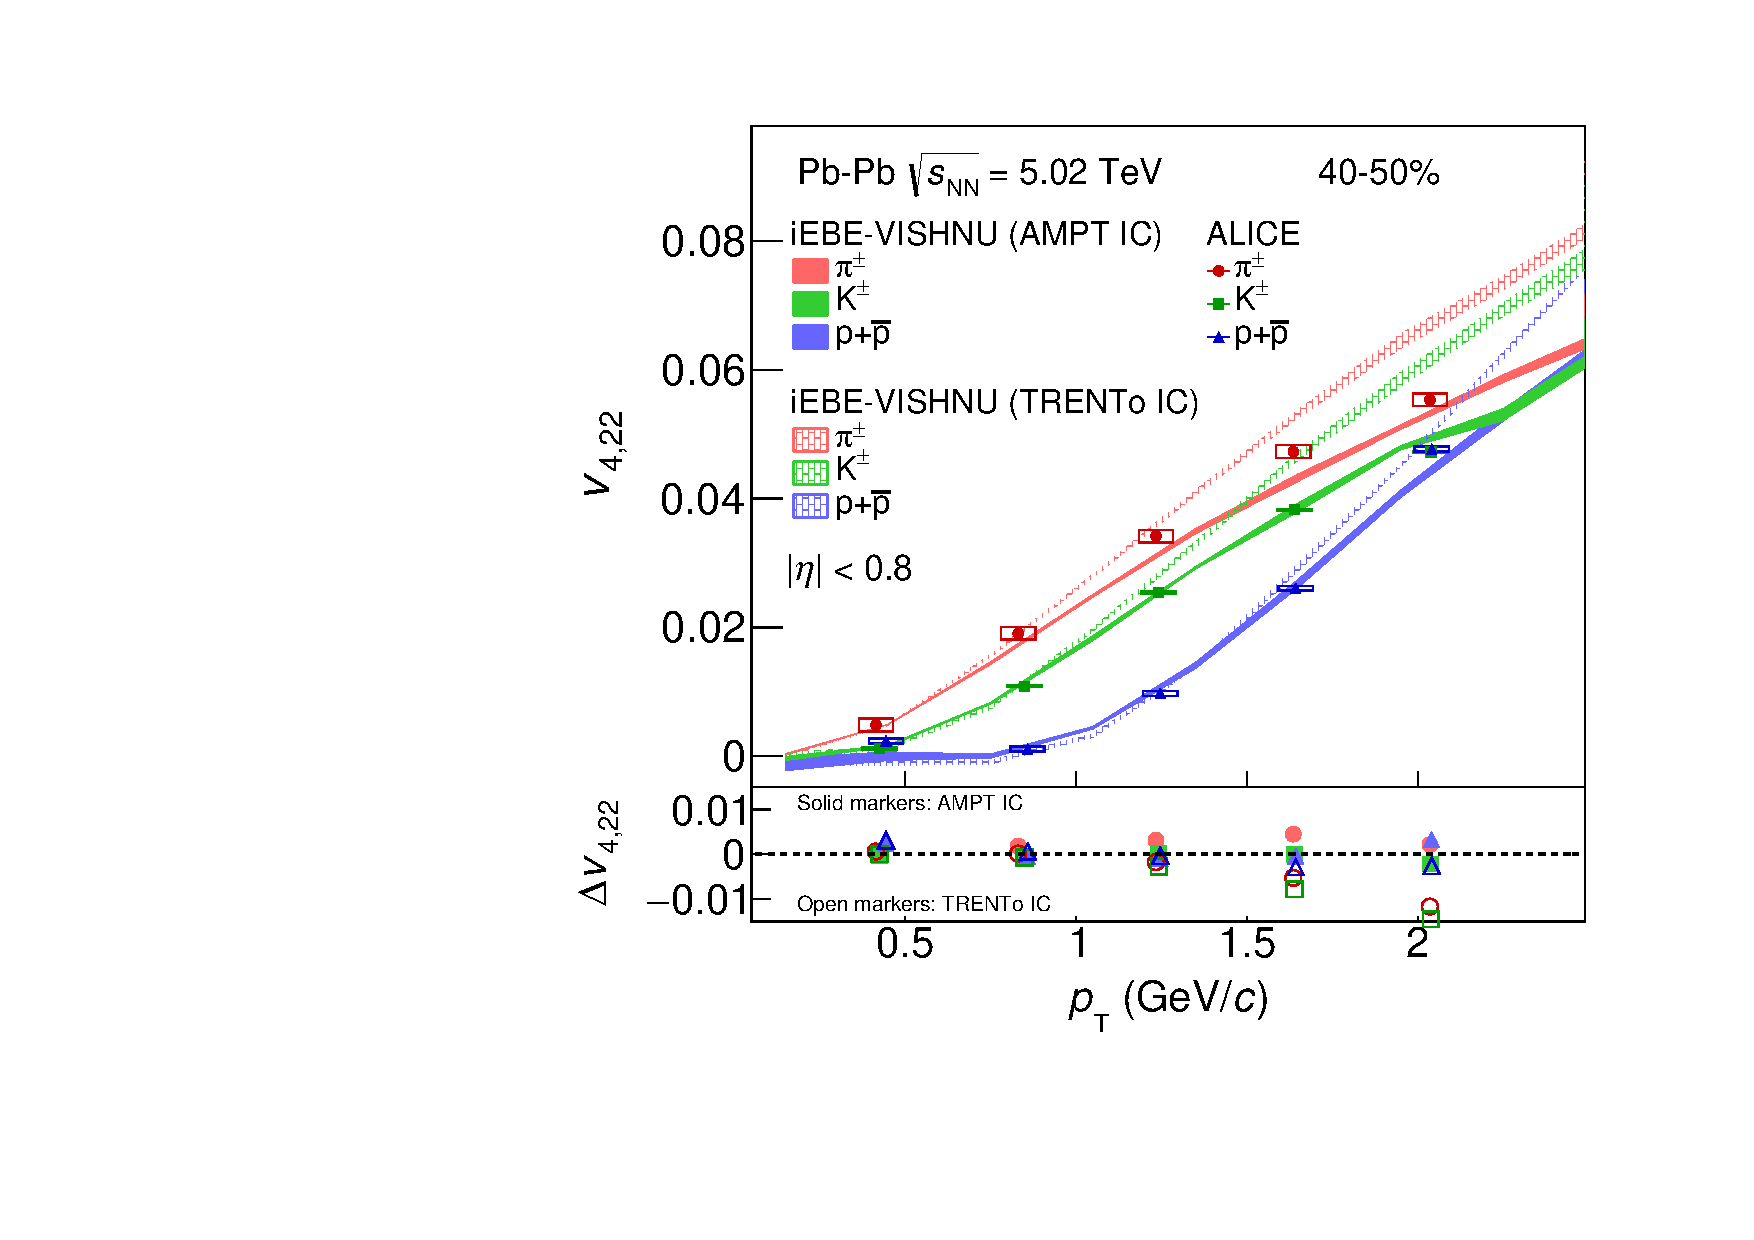
\includegraphics[scale=0.26]{figures/model/TrentoAndAMPT_v422_gap00_new_40-50_PID2.pdf}
%DIFDELCMD < 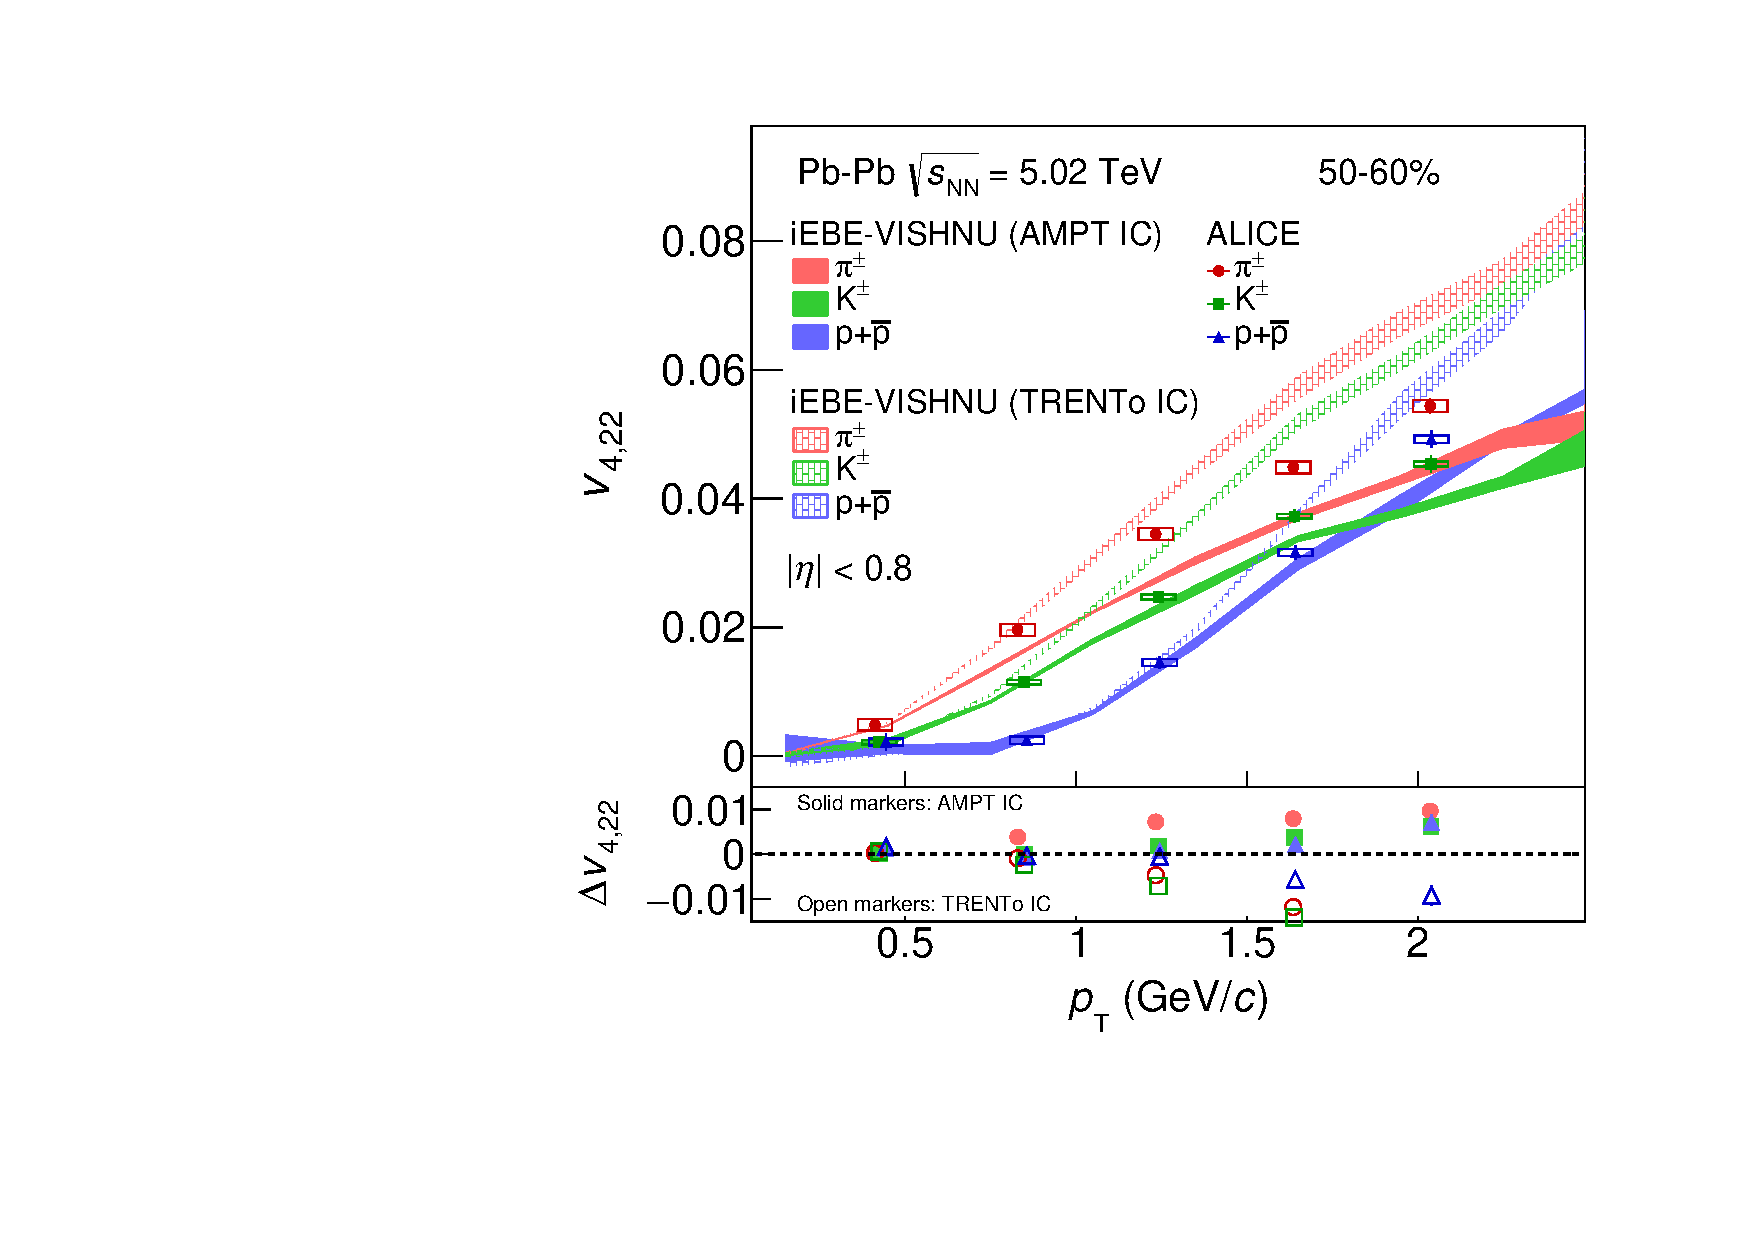
\includegraphics[scale=0.26]{figures/model/TrentoAndAMPT_v422_gap00_new_50-60_PID2.pdf}
%DIFDELCMD < %%%
\DIFdelendFL \DIFaddbeginFL 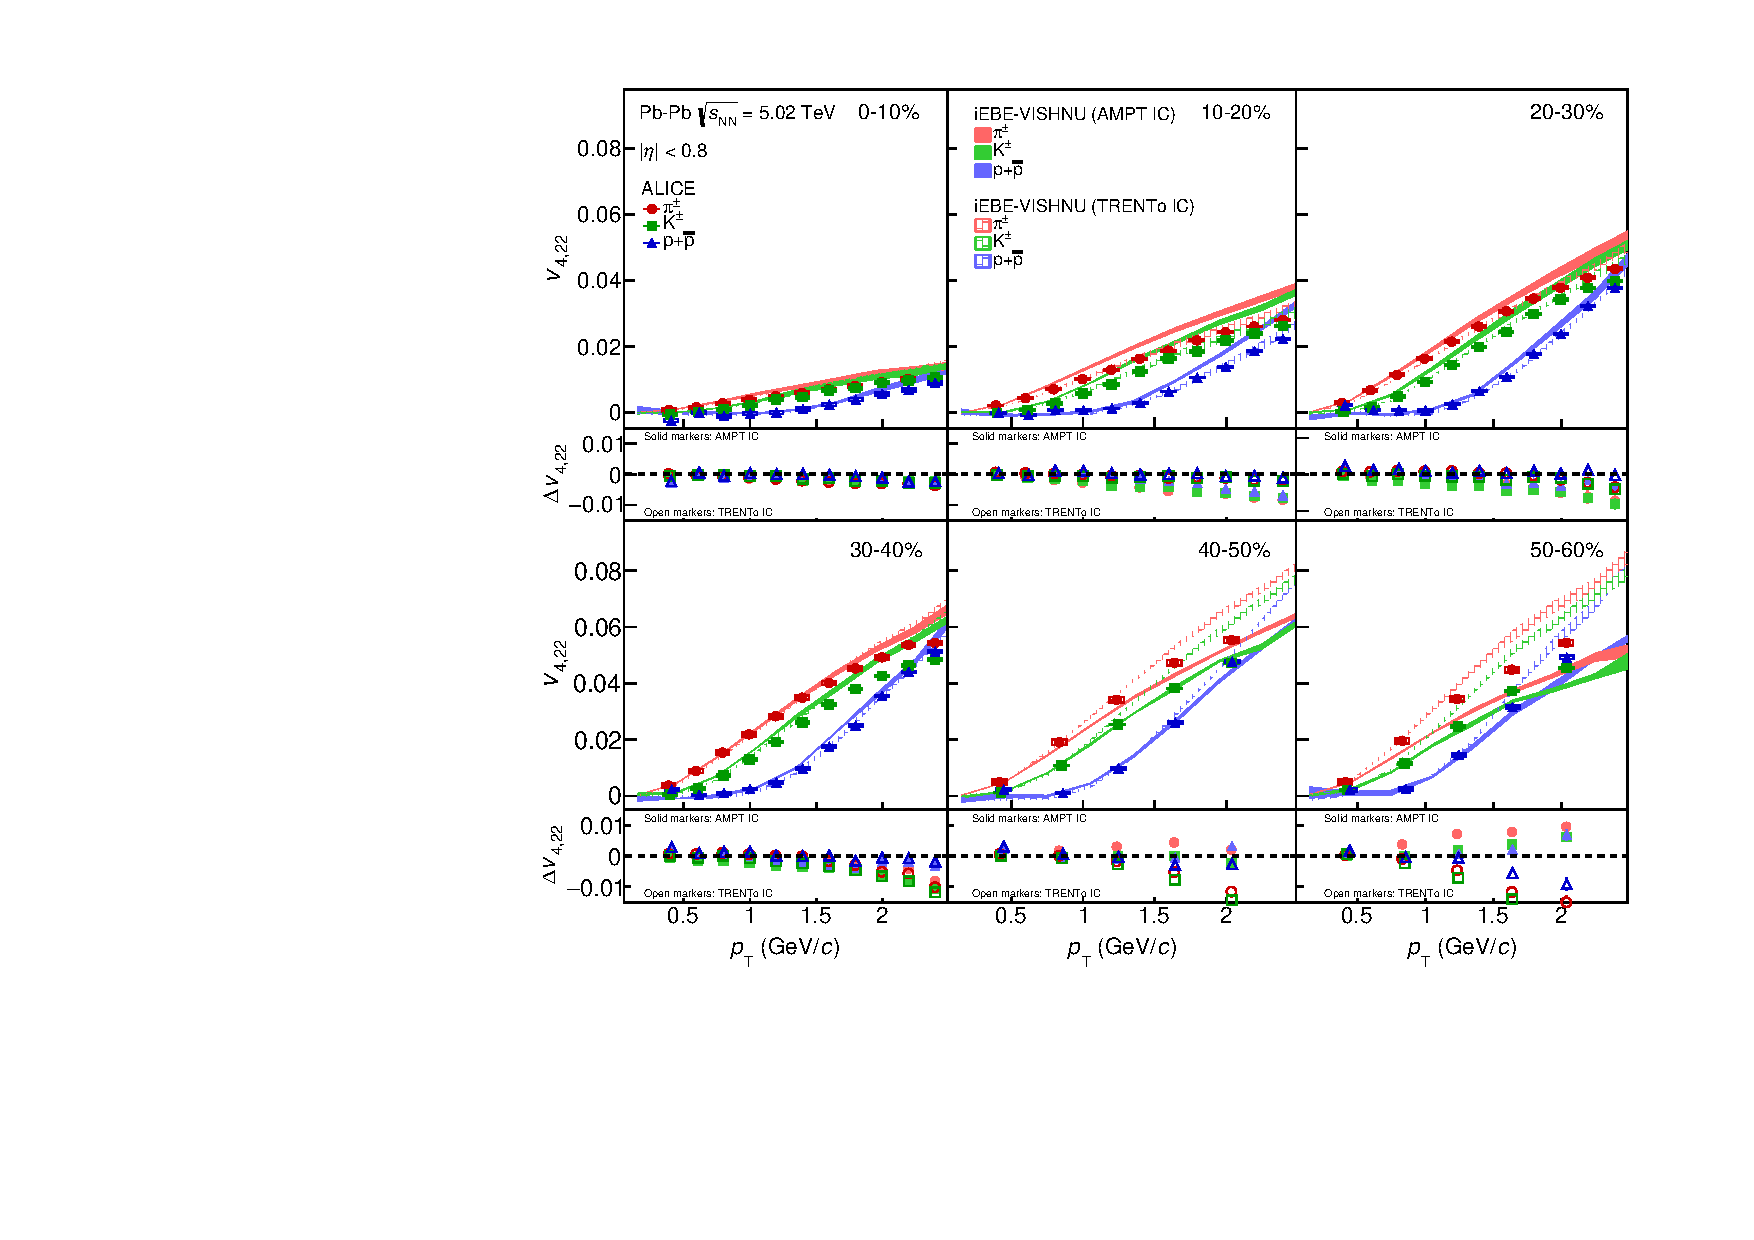
\includegraphics[scale=0.73]{figures/model/TrentoAndAMPT_v422_gap00_PID2.pdf}
%DIF > 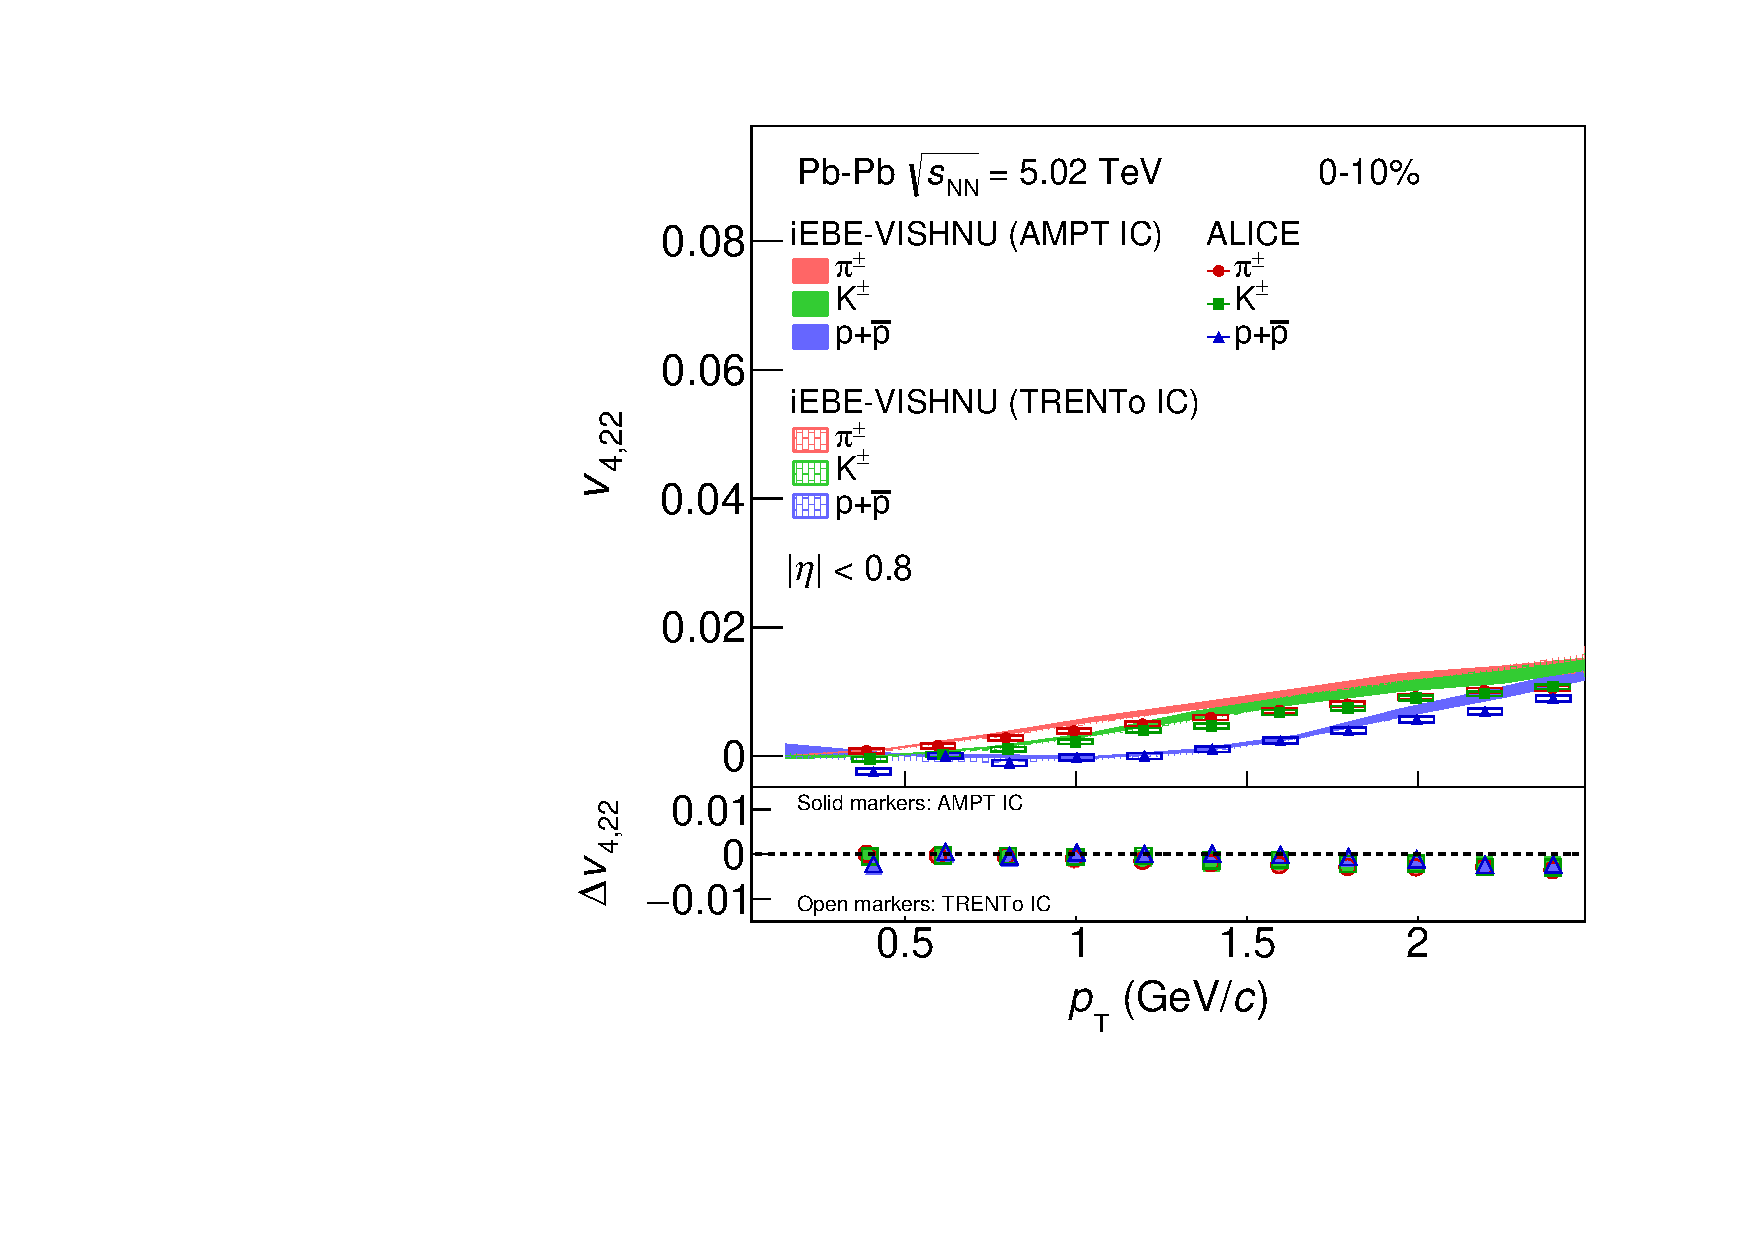
\includegraphics[scale=0.26]{figures/model/TrentoAndAMPT_v422_gap00_new_0-10_PID2.pdf}
%DIF > 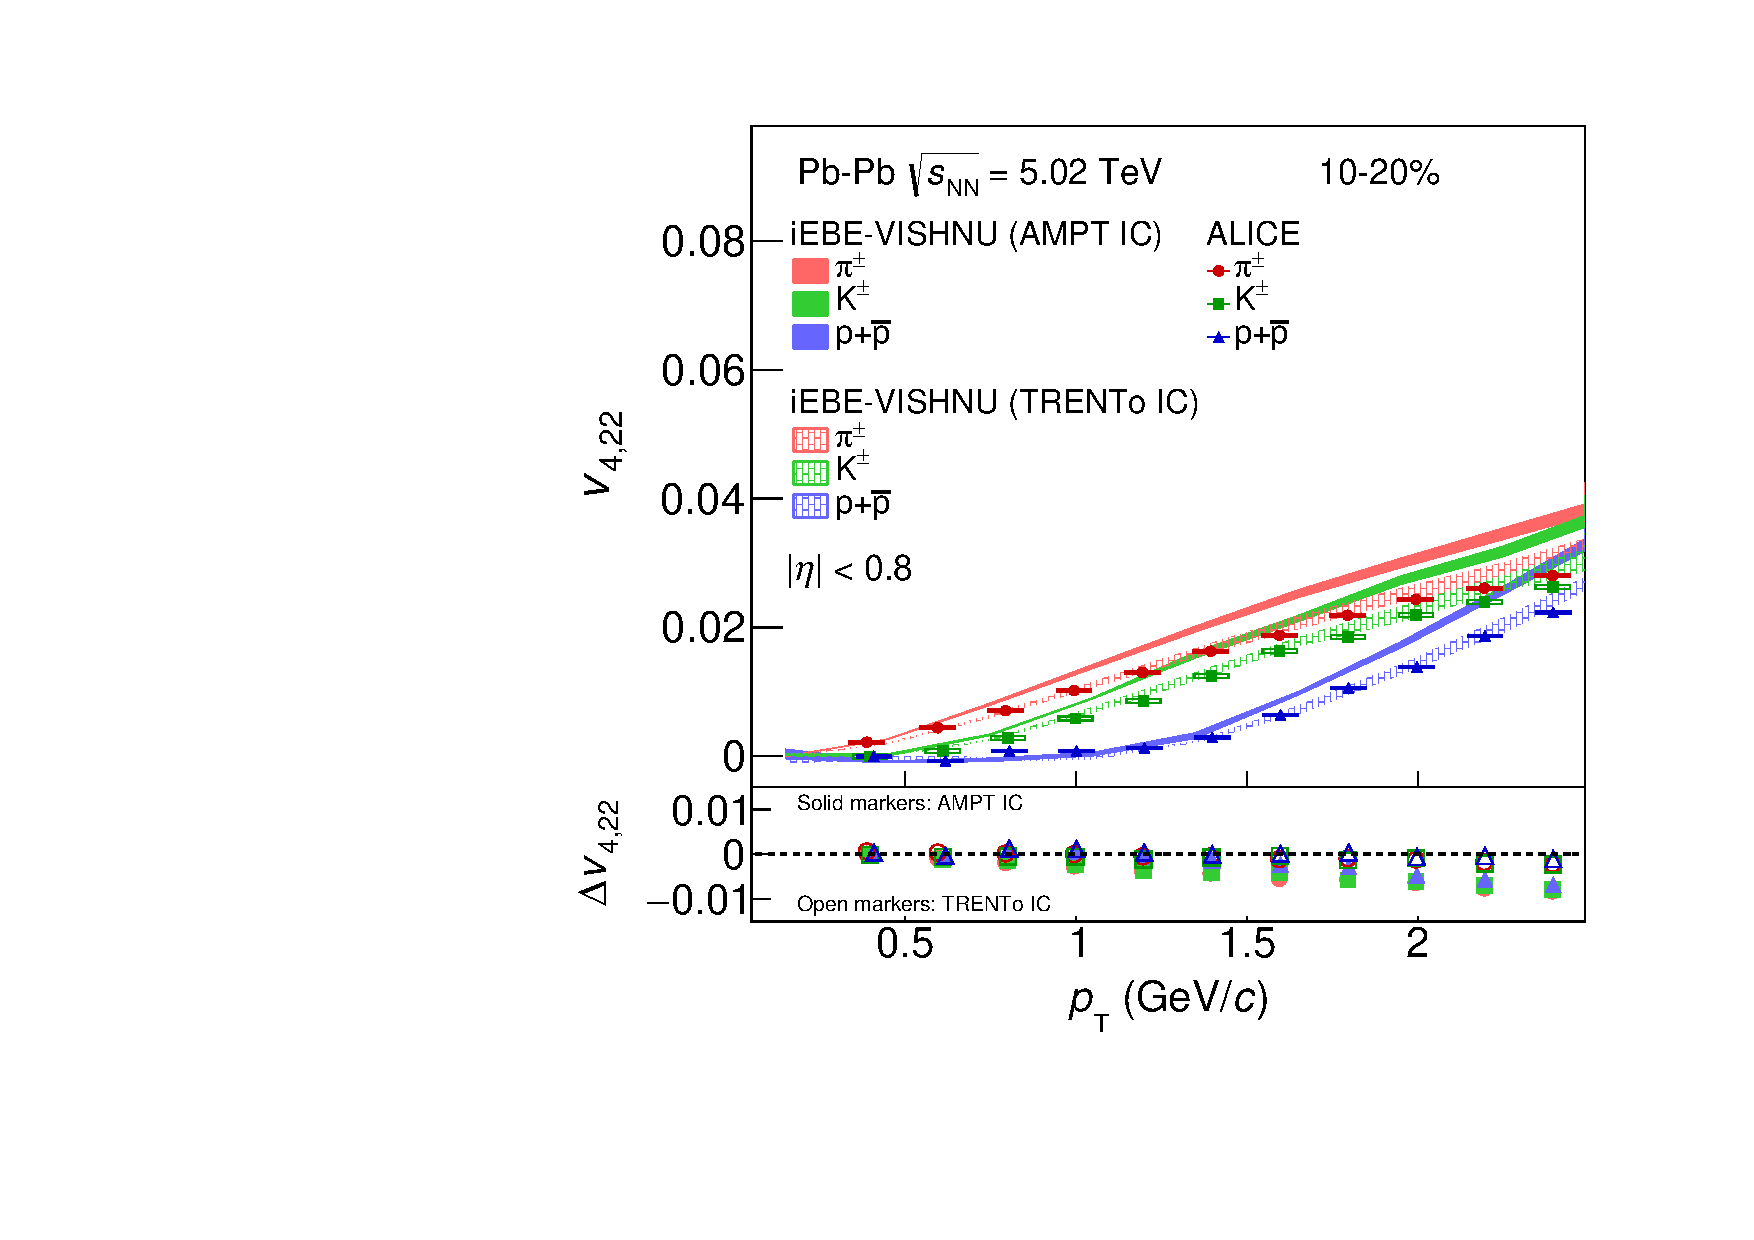
\includegraphics[scale=0.26]{figures/model/TrentoAndAMPT_v422_gap00_new_10-20_PID2.pdf}
%DIF > 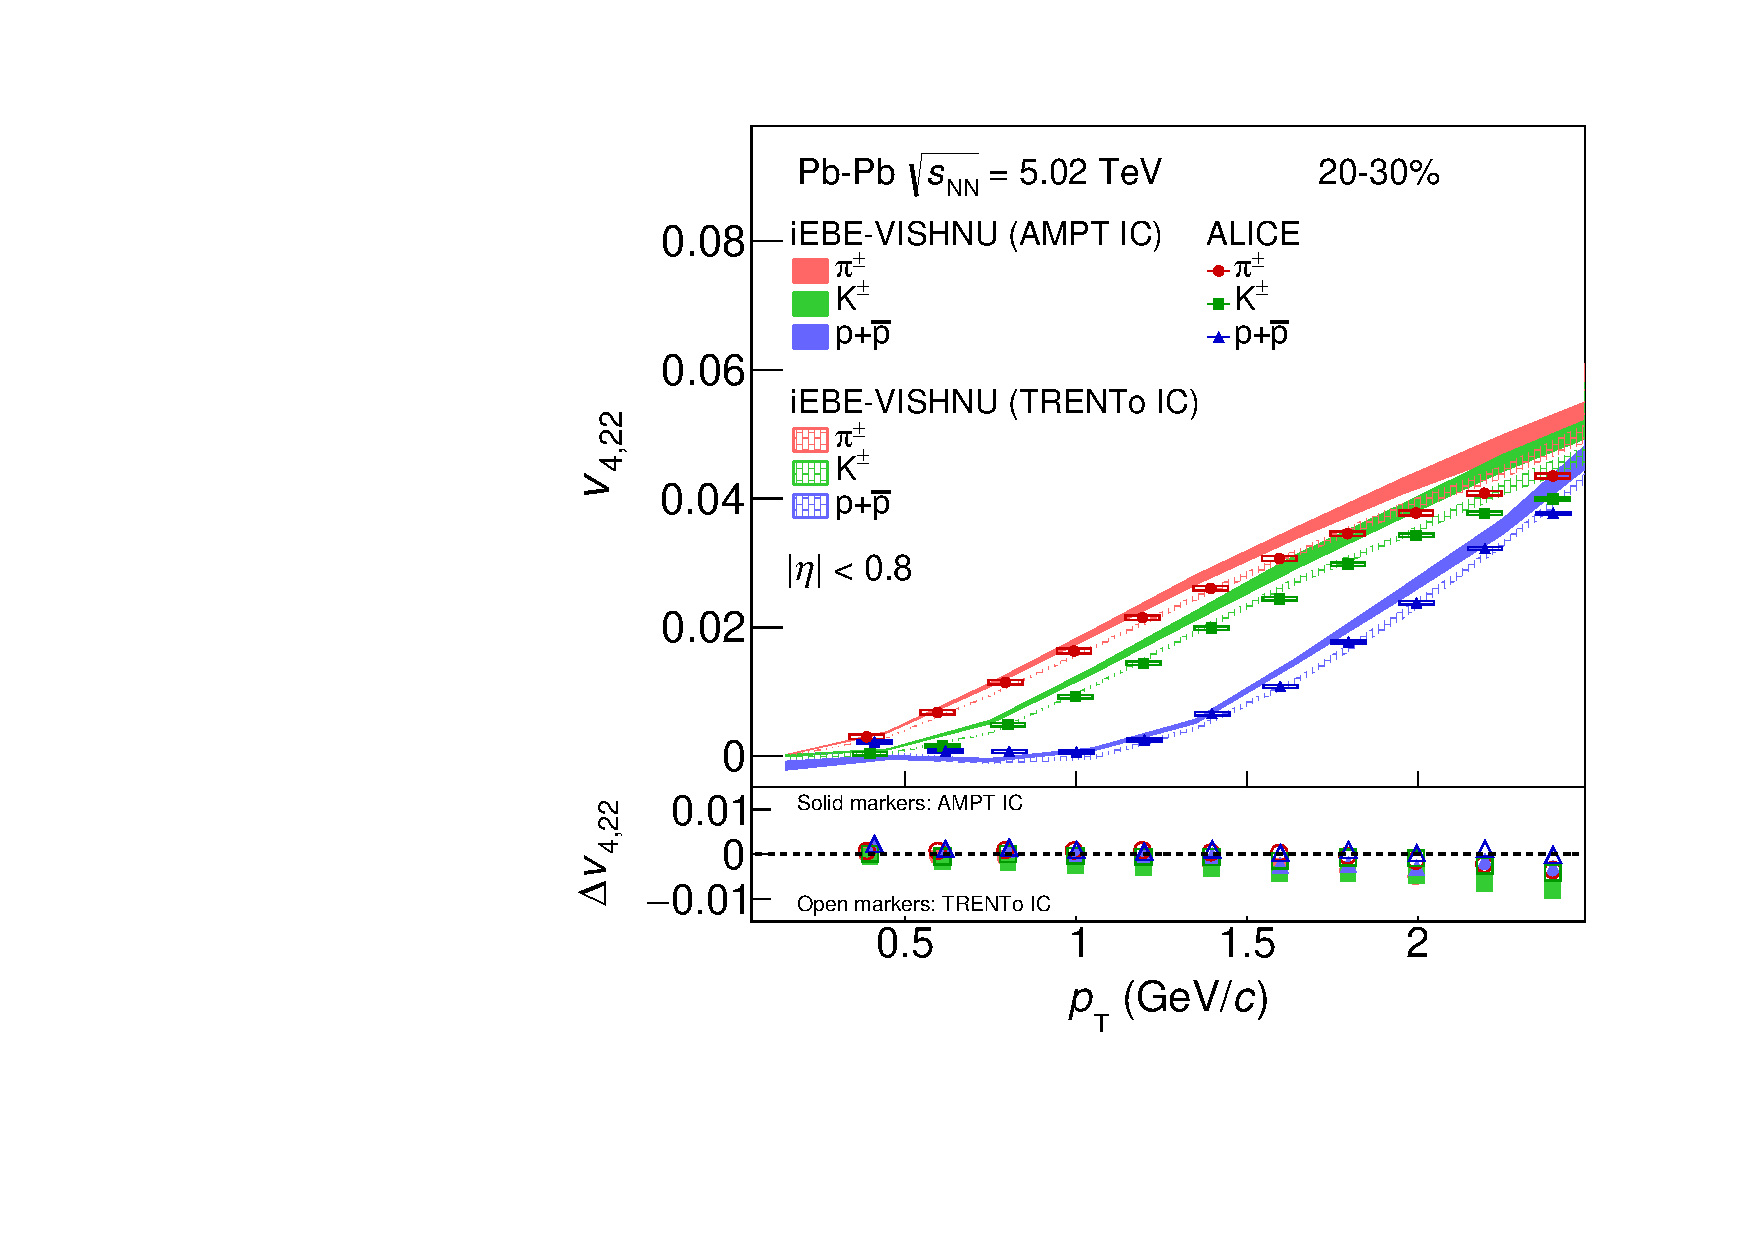
\includegraphics[scale=0.26]{figures/model/TrentoAndAMPT_v422_gap00_new_20-30_PID2.pdf}
%DIF > 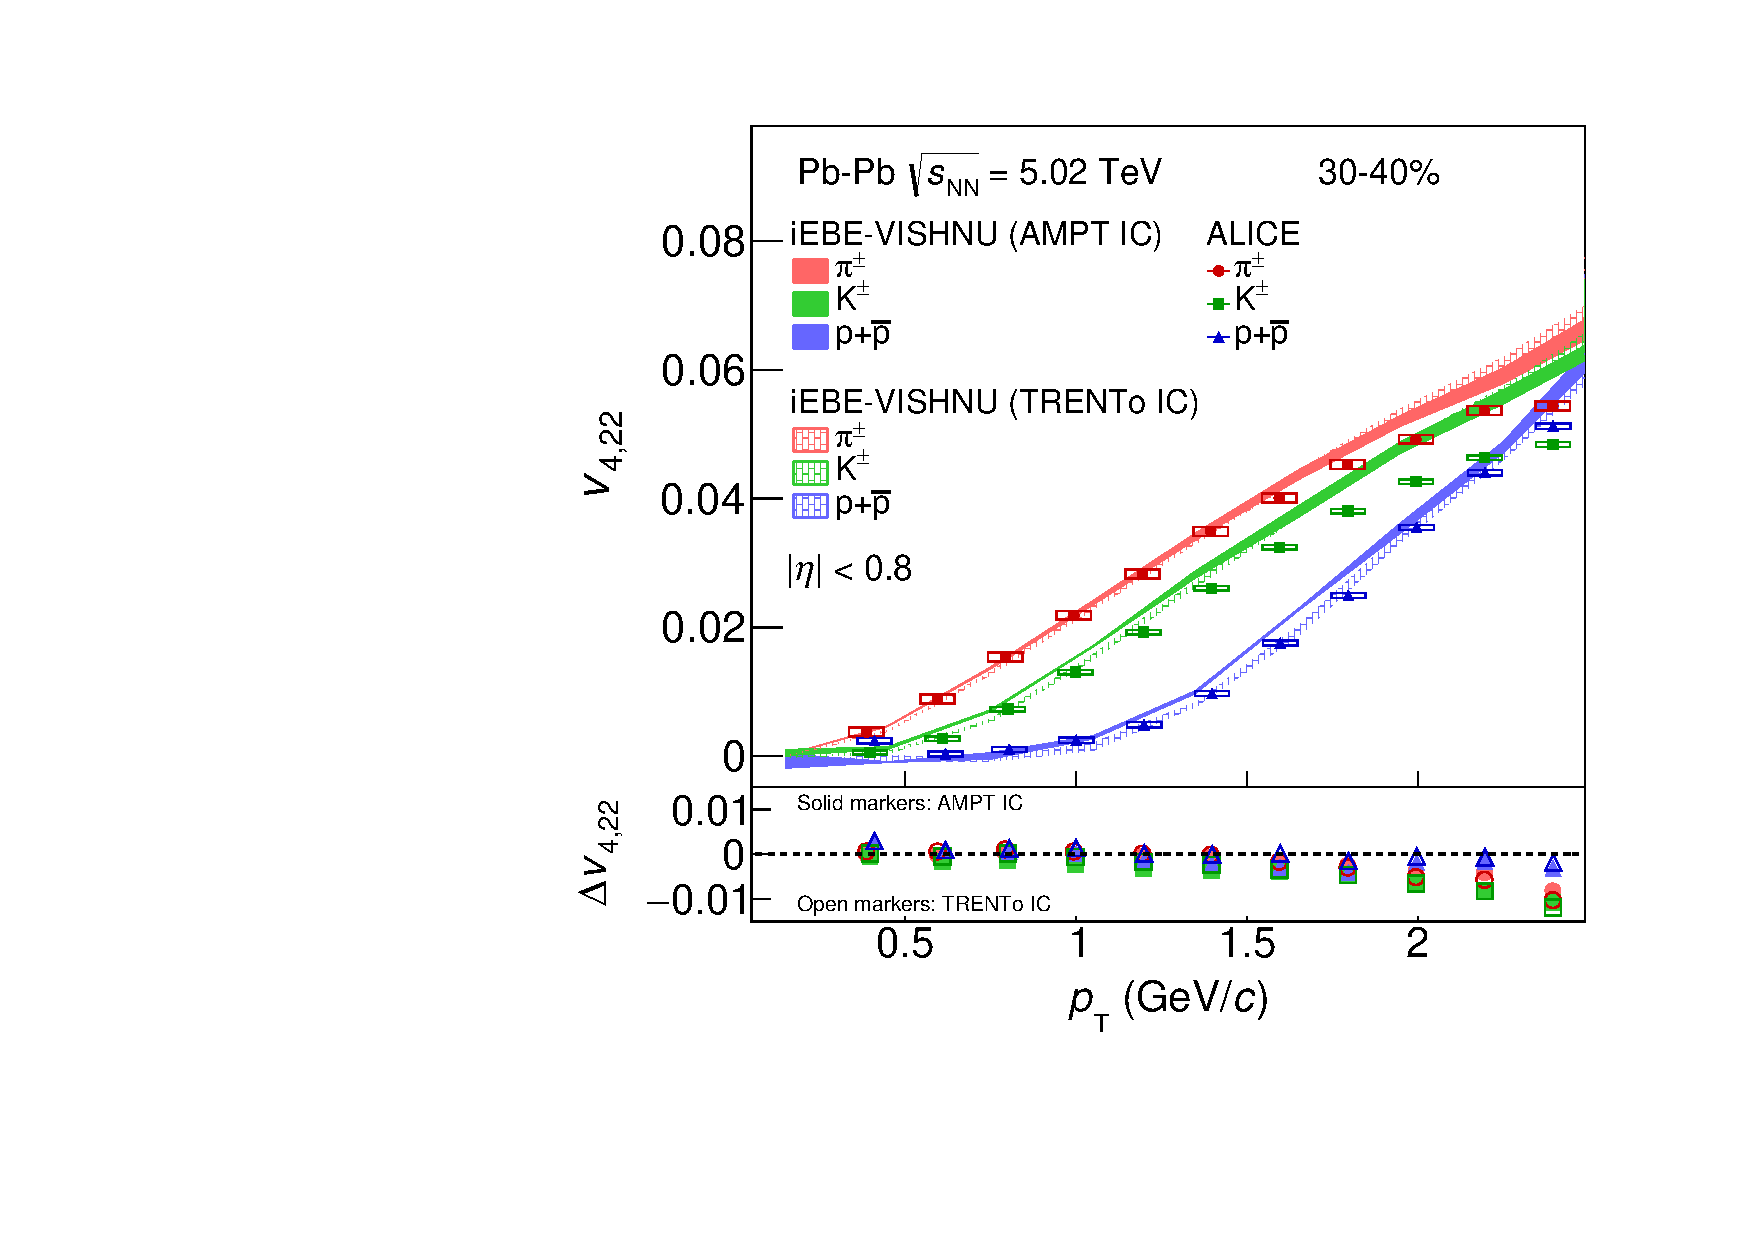
\includegraphics[scale=0.26]{figures/model/TrentoAndAMPT_v422_gap00_new_30-40_PID2.pdf}
%DIF > 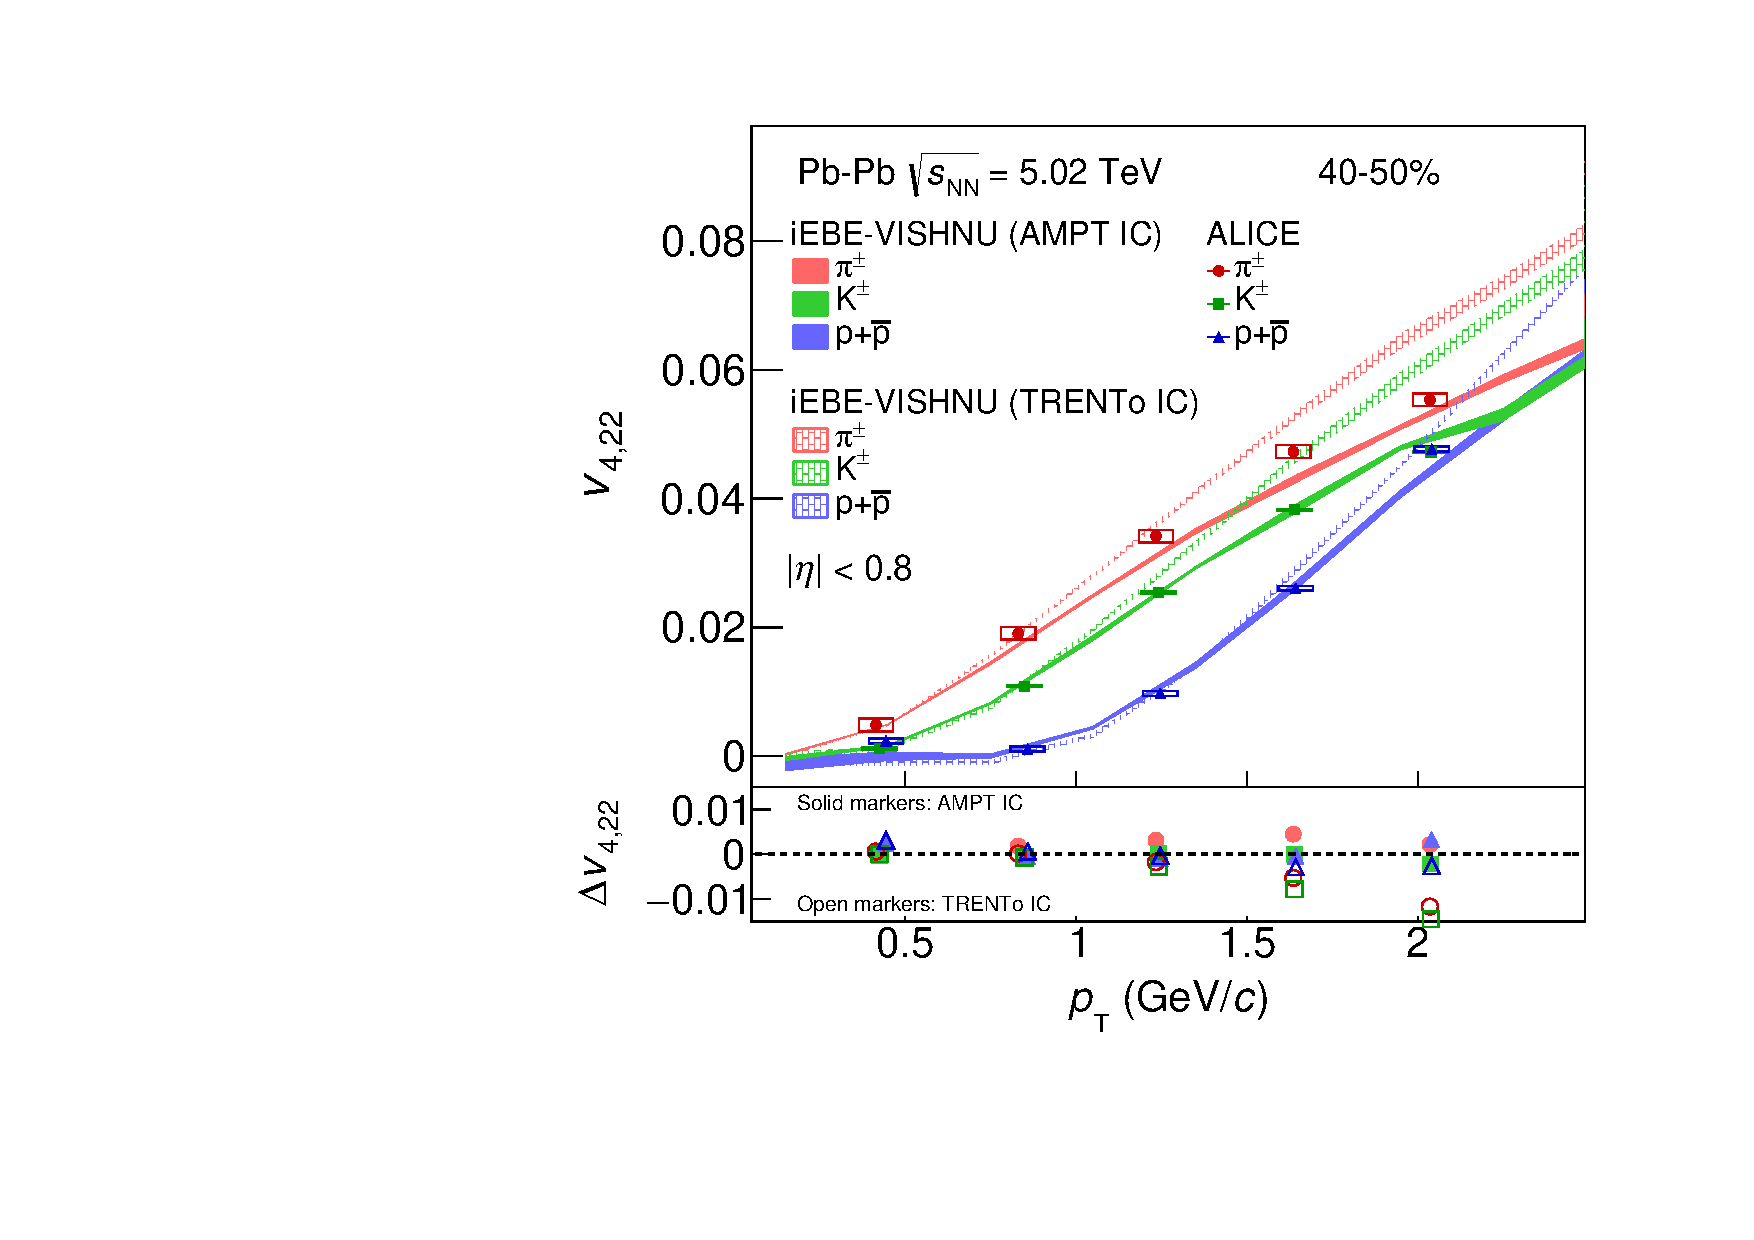
\includegraphics[scale=0.26]{figures/model/TrentoAndAMPT_v422_gap00_new_40-50_PID2.pdf}
%DIF > 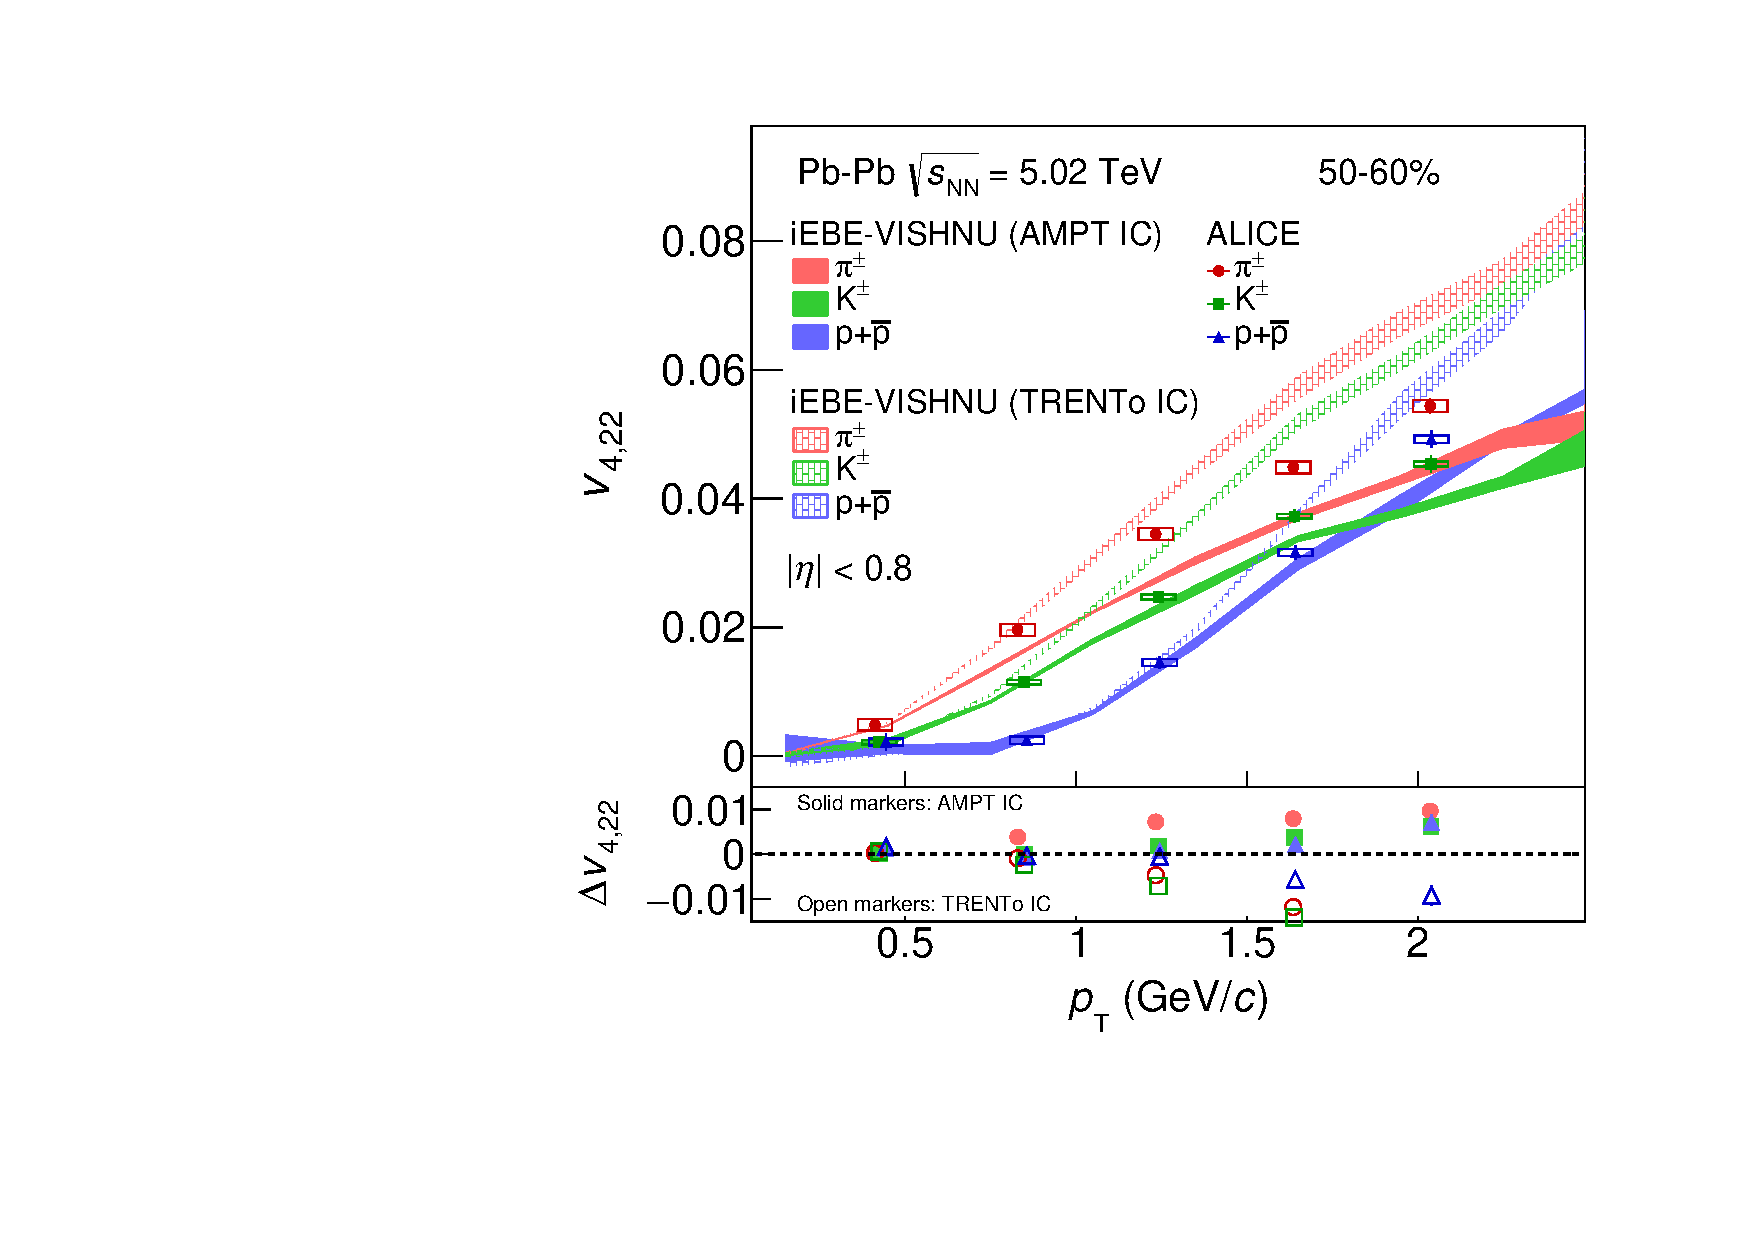
\includegraphics[scale=0.26]{figures/model/TrentoAndAMPT_v422_gap00_new_50-60_PID2.pdf}
\DIFaddendFL \end{center}
\caption{The \pT-differential $v_{4,22}$ for different particle species in 10-20\% up to 50-60\% centrality intervals of Pb--Pb collisions at \sNN compared with iEBE-VISHNU hybrid models with two different sets of initial parameters: AMPT initial conditions ($\eta/s$= 0.08 and $\zeta/s$ = 0) shown in solid bands and TRENTo initial conditions ($\eta/s({\rm T})$ and $\zeta/s({\rm T})$) in hatched bands. The bottom panels show the difference between the measurements and each model.}
\label{v422_model}
\end{figure}


\begin{figure}[!htb]
\begin{center}
\DIFdelbeginFL %DIFDELCMD < 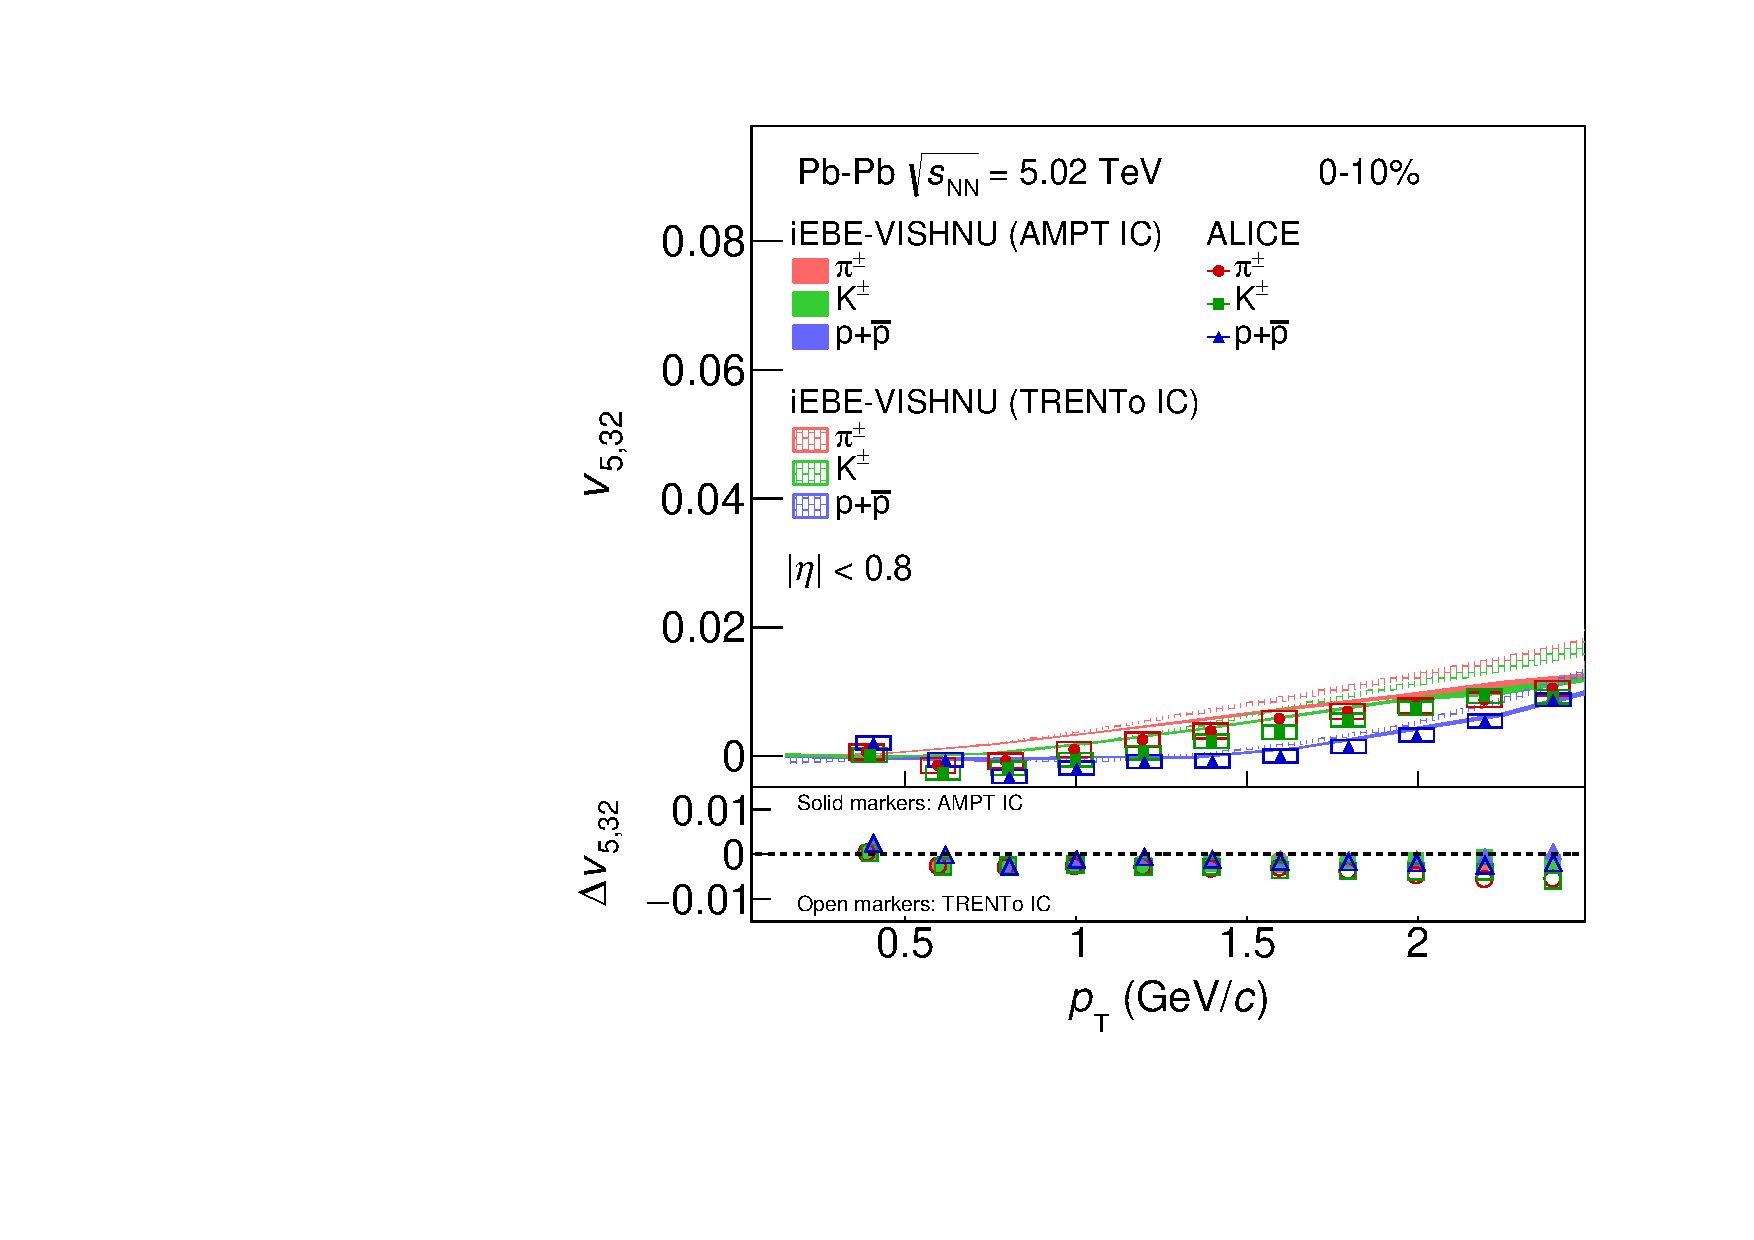
\includegraphics[scale=0.26]{figures/model/TrentoAndAMPT_v523_gap00_new_0-10_PID2.pdf}
%DIFDELCMD < 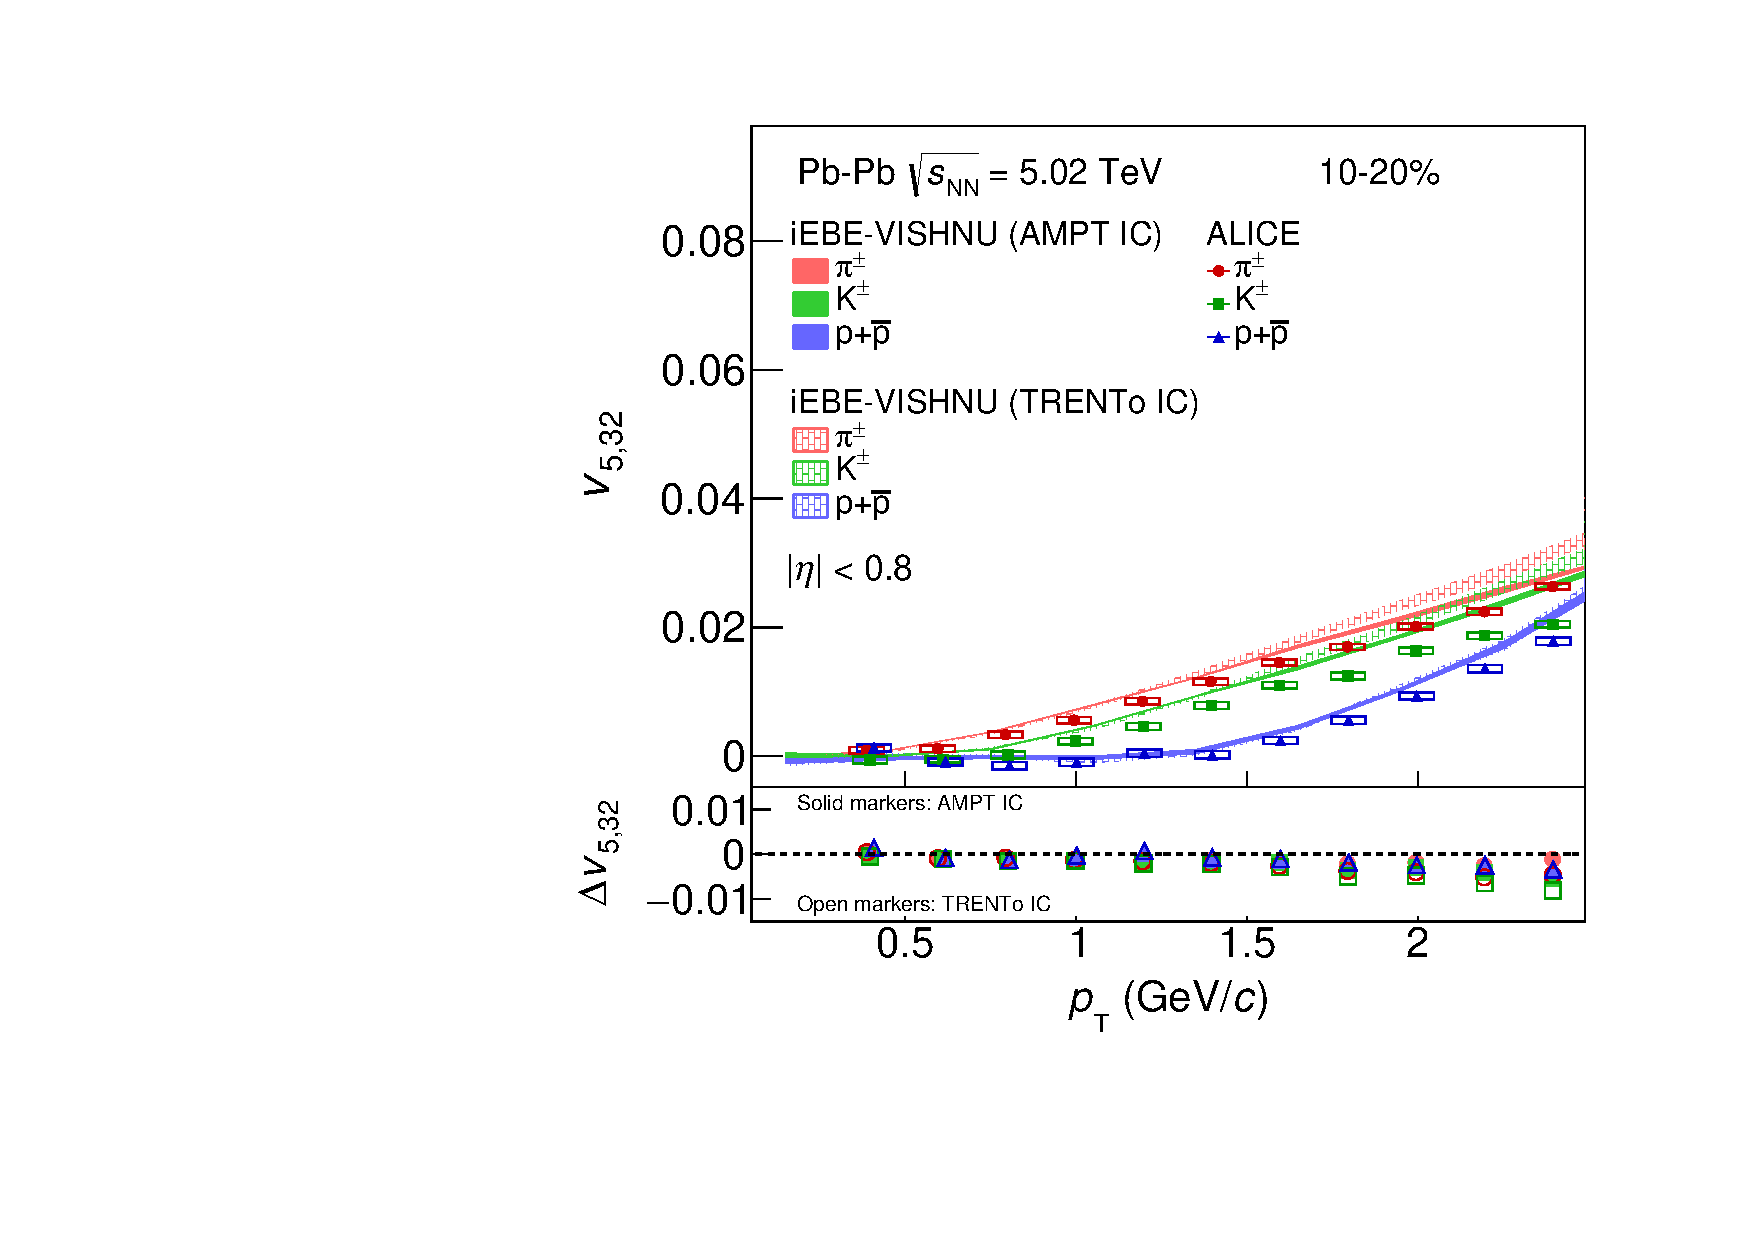
\includegraphics[scale=0.26]{figures/model/TrentoAndAMPT_v523_gap00_new_10-20_PID2.pdf}
%DIFDELCMD < 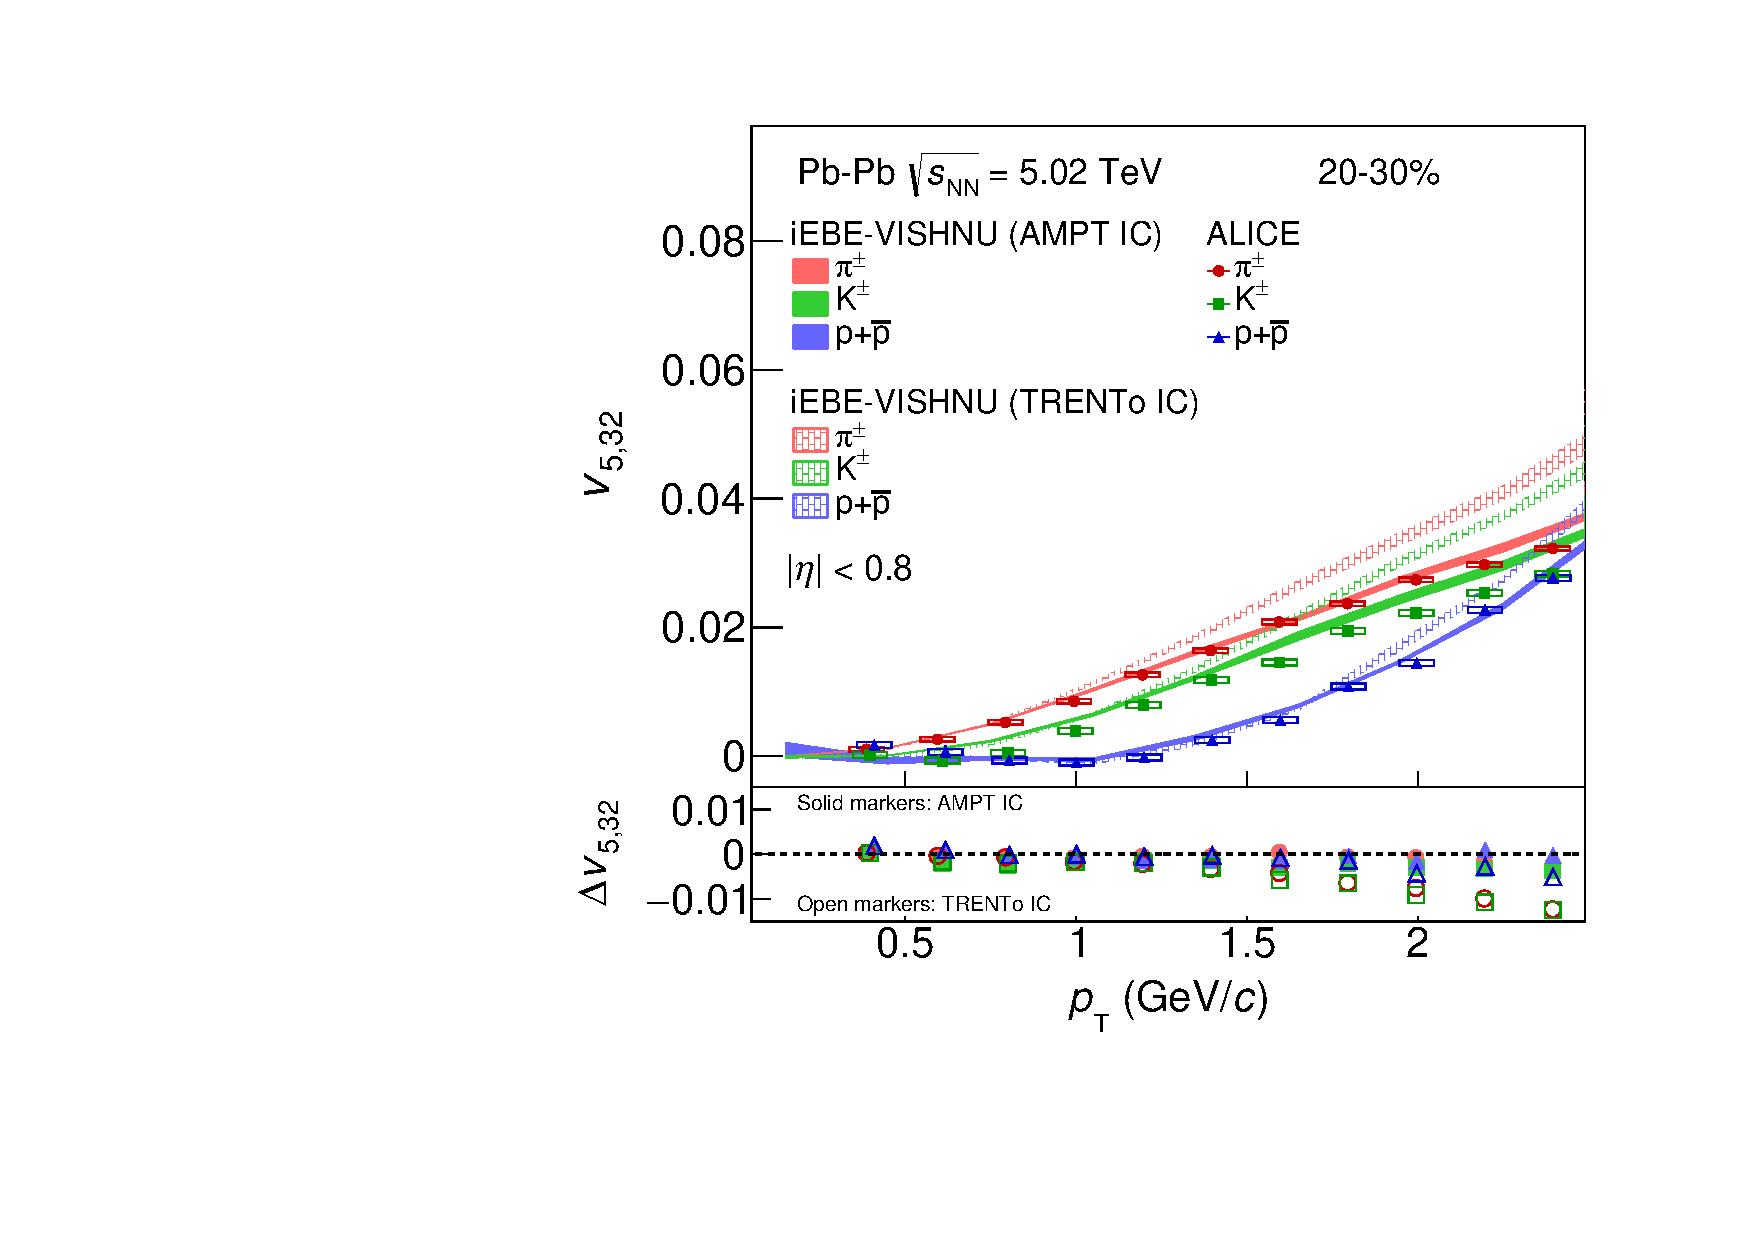
\includegraphics[scale=0.26]{figures/model/TrentoAndAMPT_v523_gap00_new_20-30_PID2.pdf}
%DIFDELCMD < 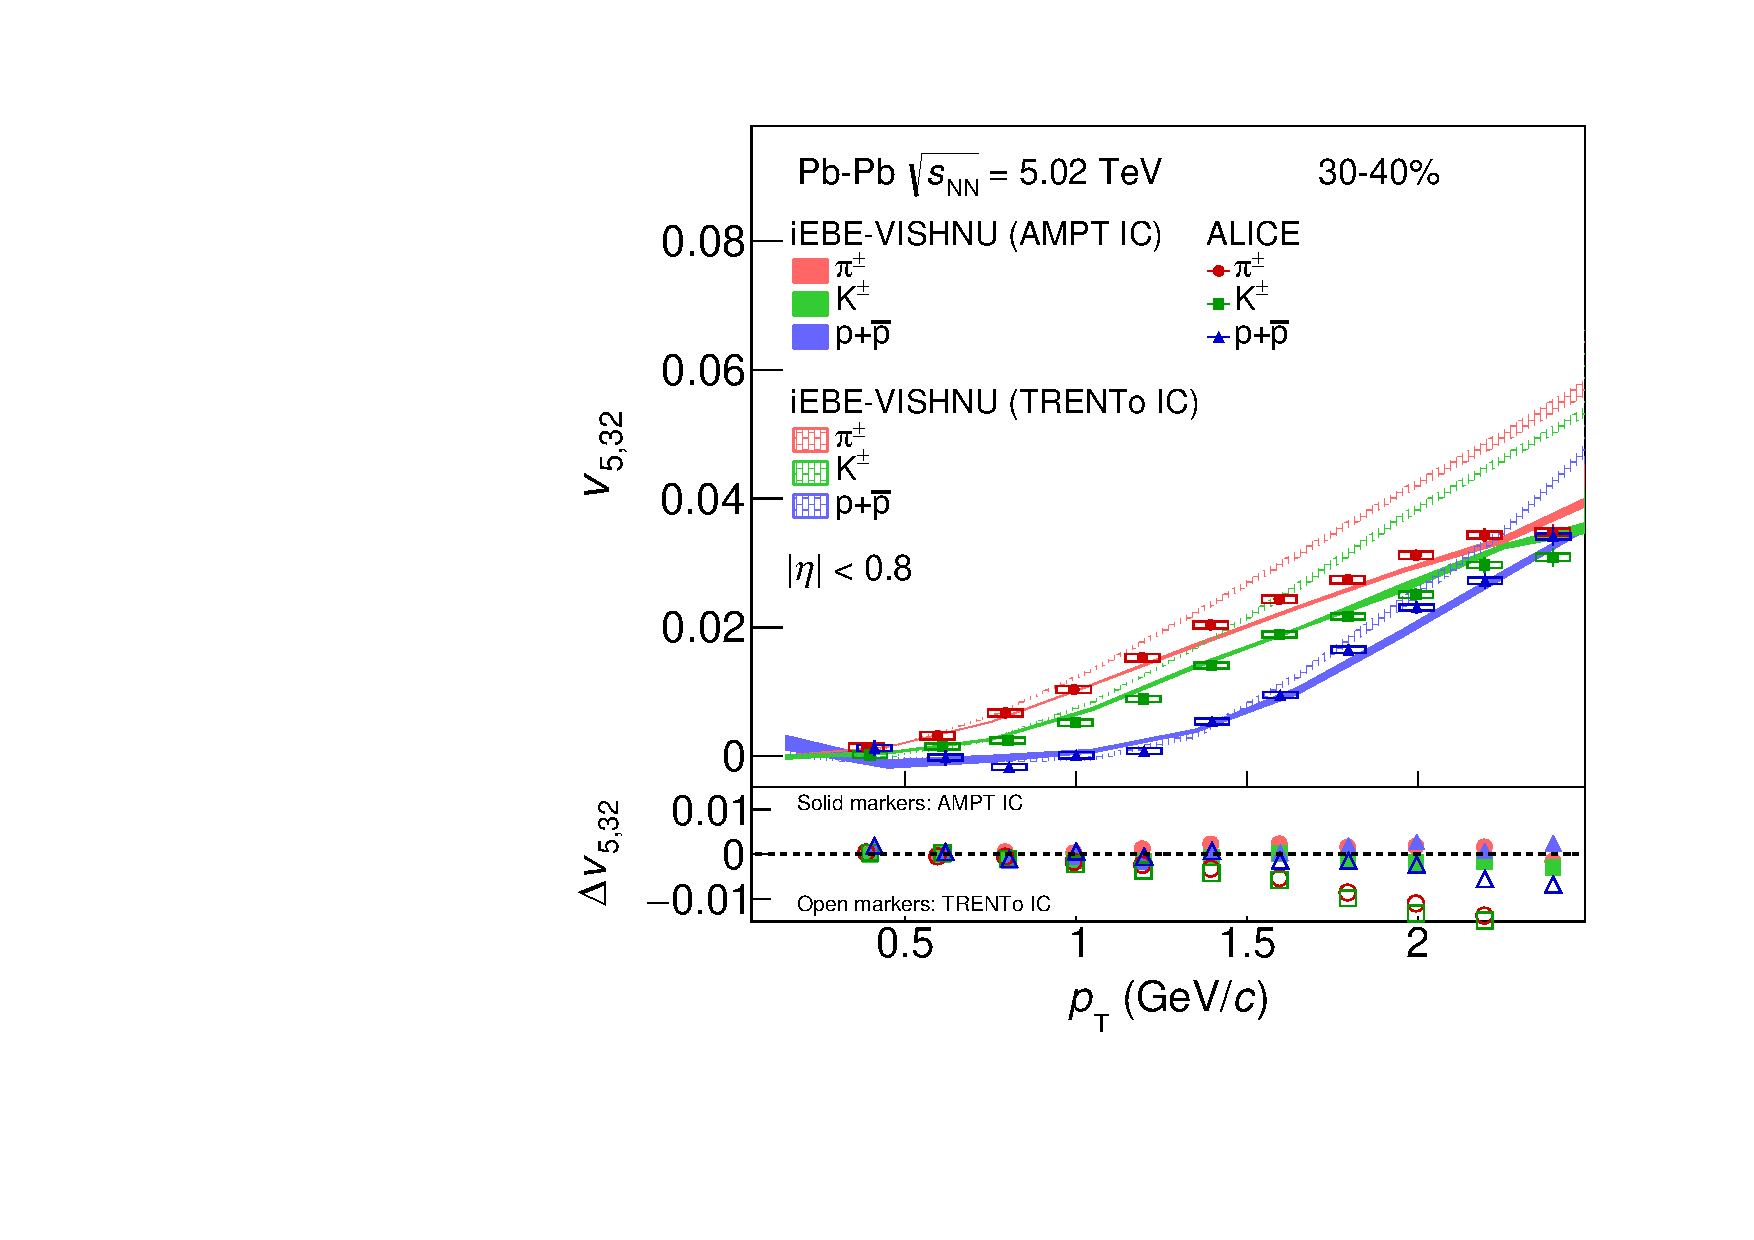
\includegraphics[scale=0.26]{figures/model/TrentoAndAMPT_v523_gap00_new_30-40_PID2.pdf}
%DIFDELCMD < 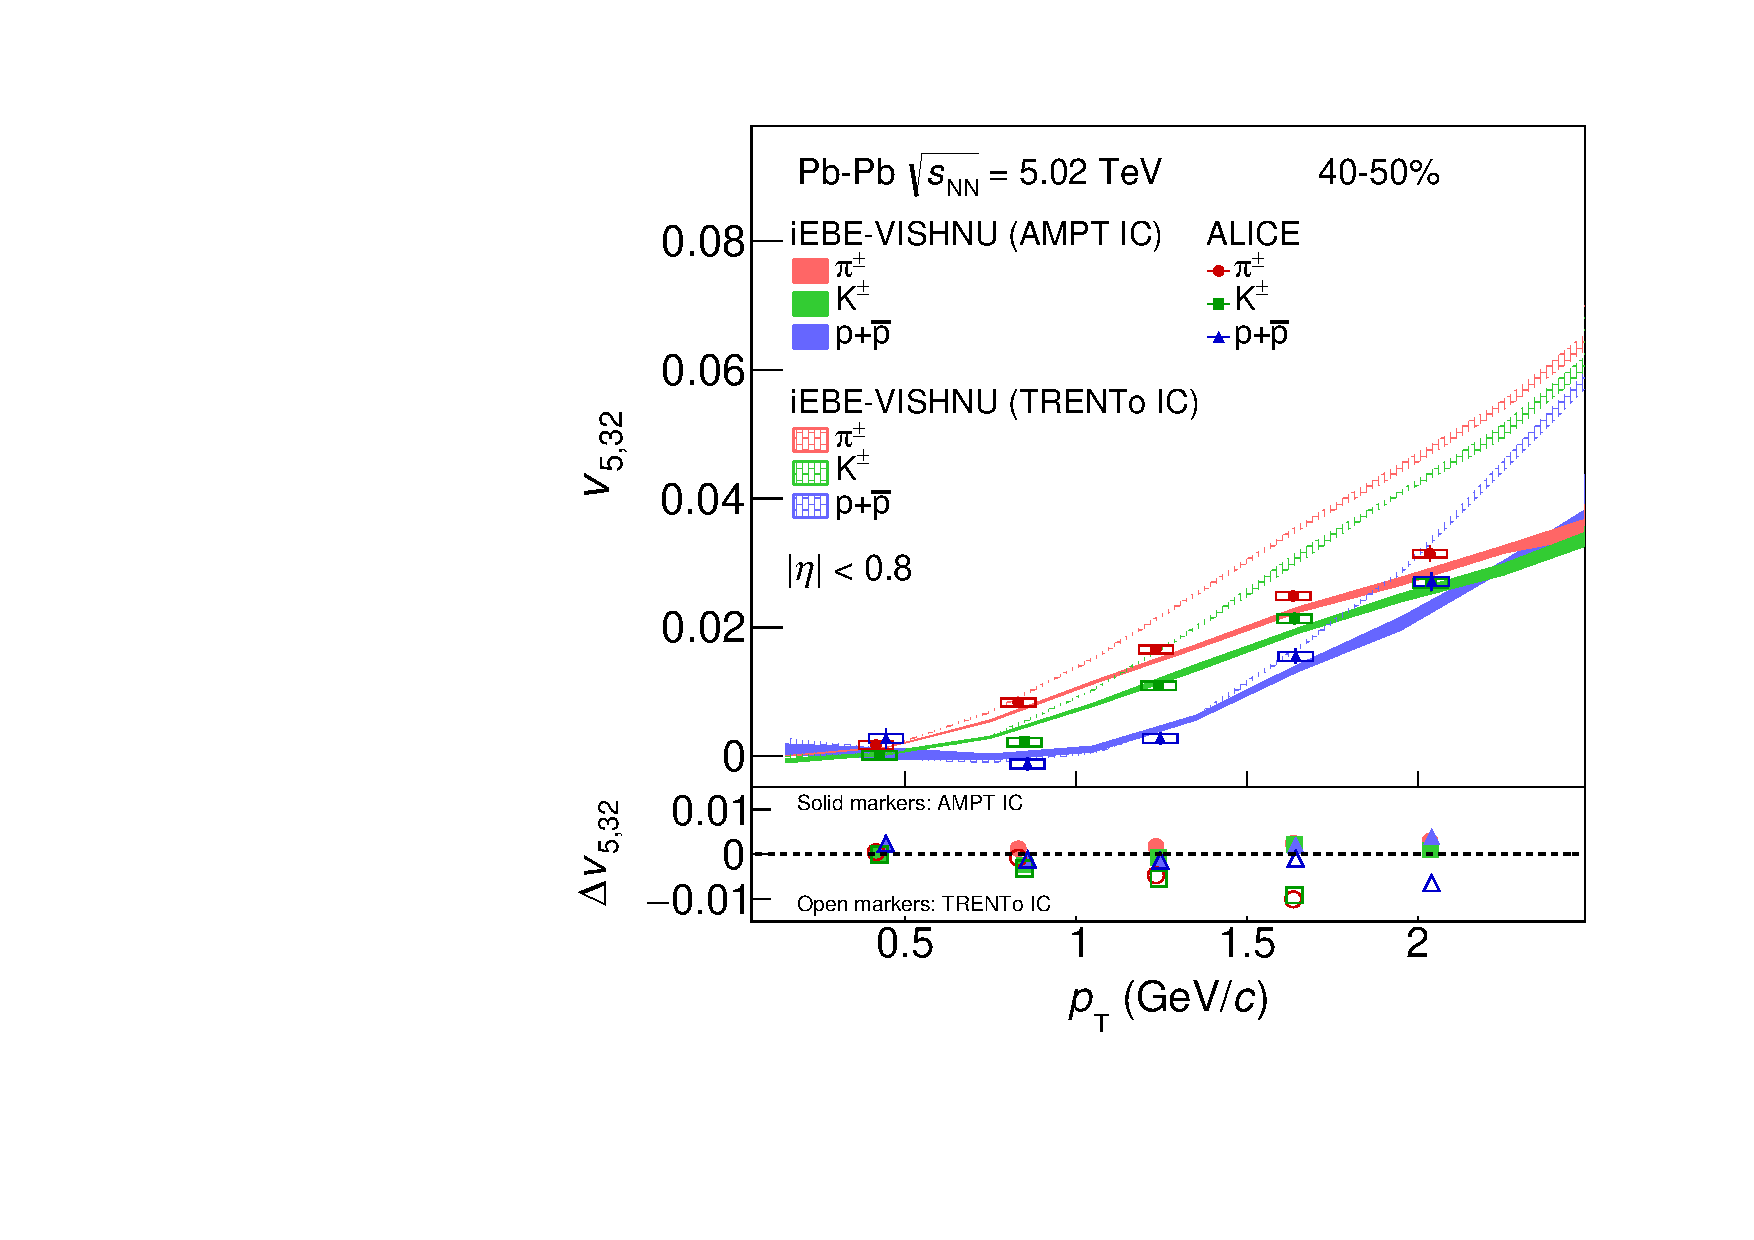
\includegraphics[scale=0.26]{figures/model/TrentoAndAMPT_v523_gap00_new_40-50_PID2.pdf}
%DIFDELCMD < 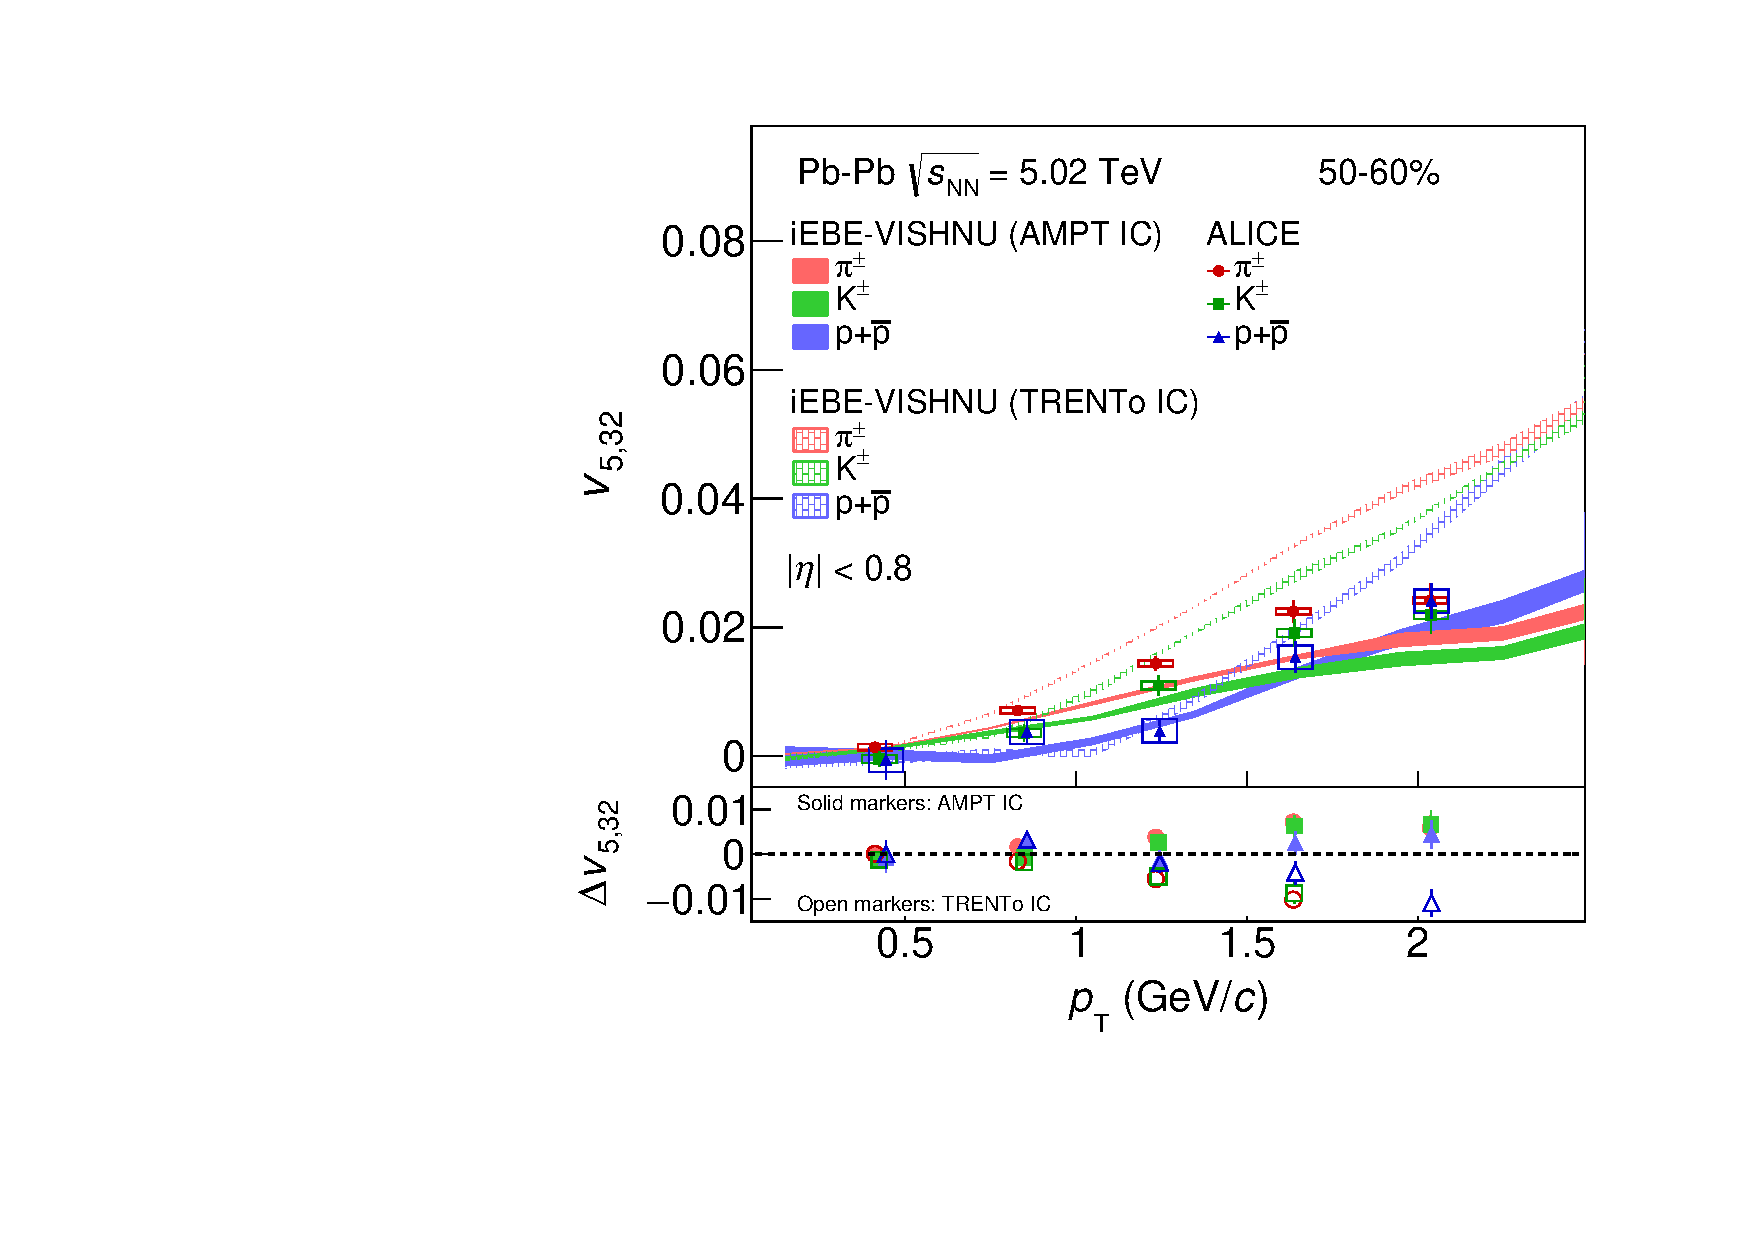
\includegraphics[scale=0.26]{figures/model/TrentoAndAMPT_v523_gap00_new_50-60_PID2.pdf}
%DIFDELCMD < %%%
\DIFdelendFL \DIFaddbeginFL 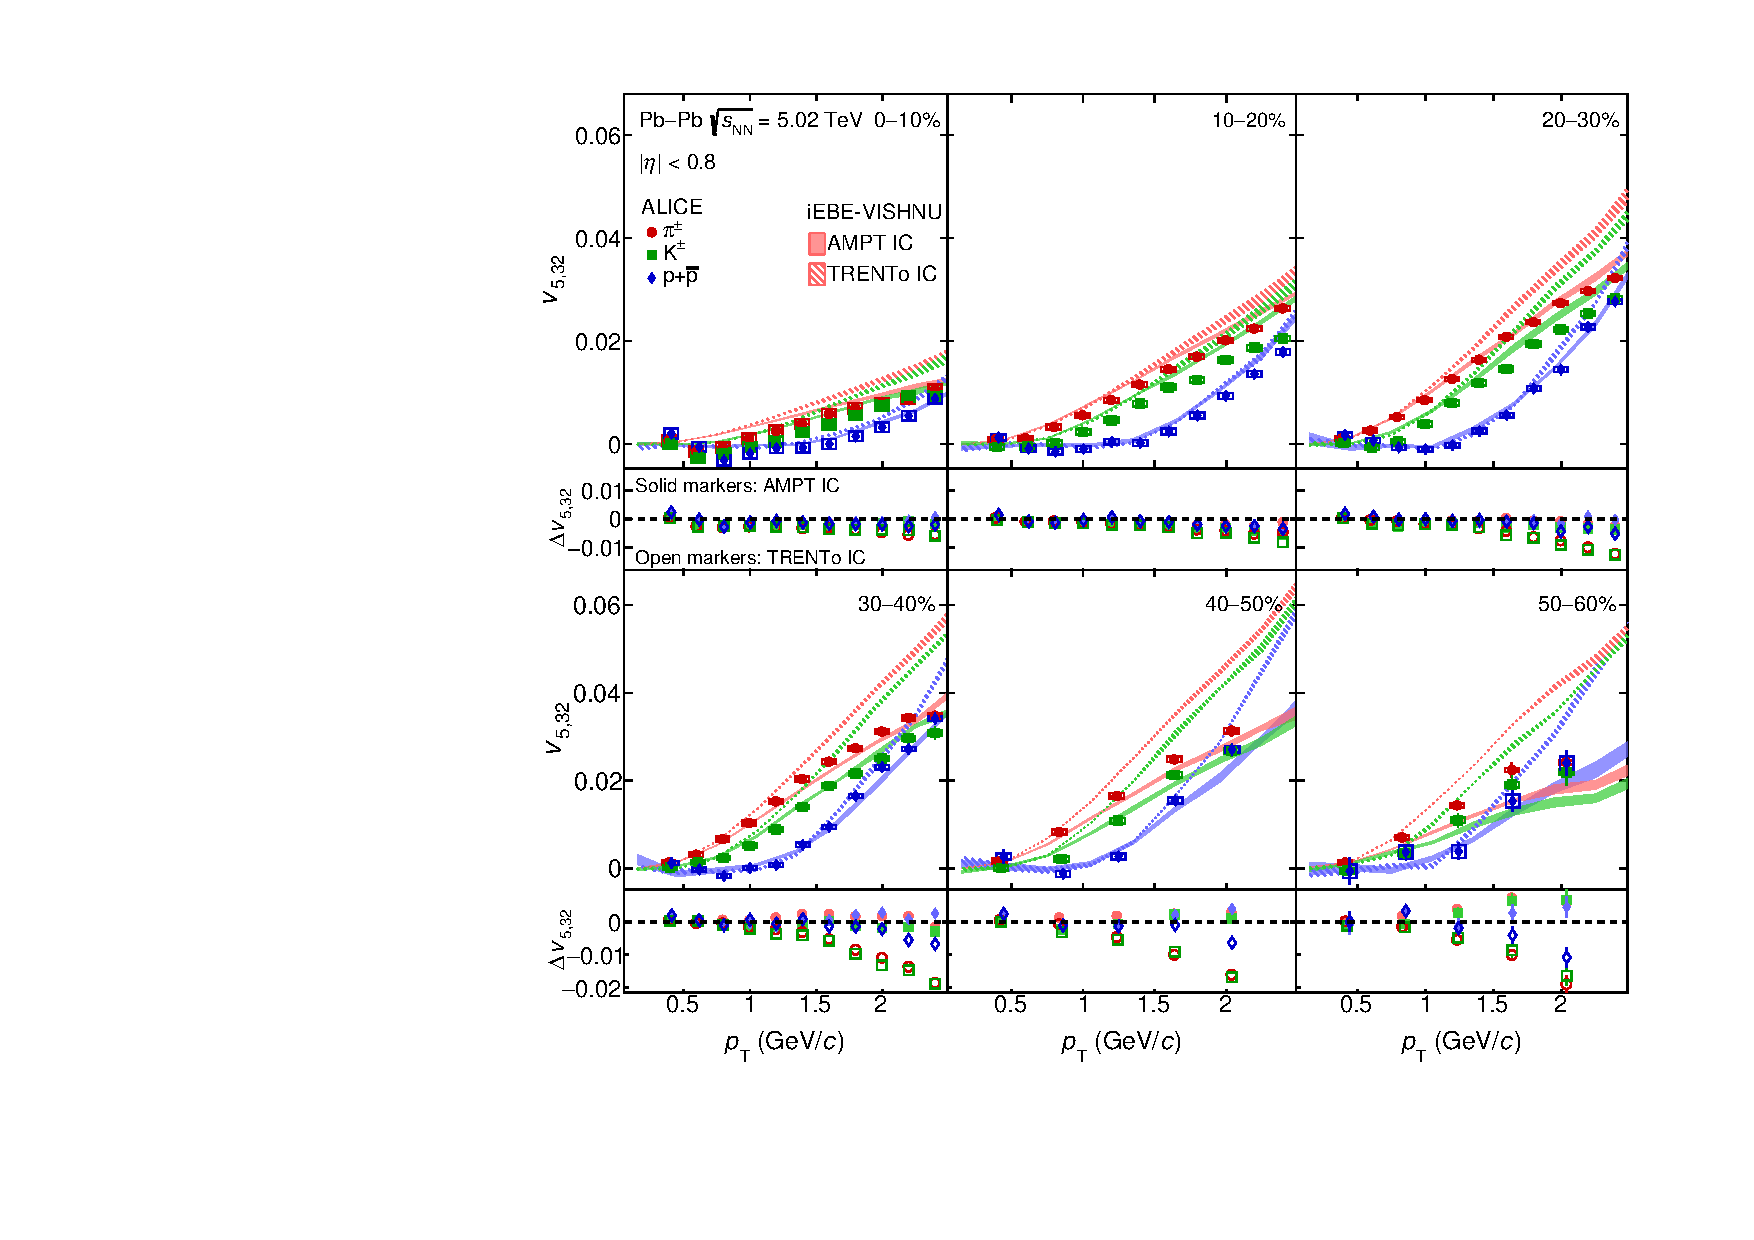
\includegraphics[scale=0.73]{figures/model/TrentoAndAMPT_v523_gap00_PID2.pdf}
%DIF > 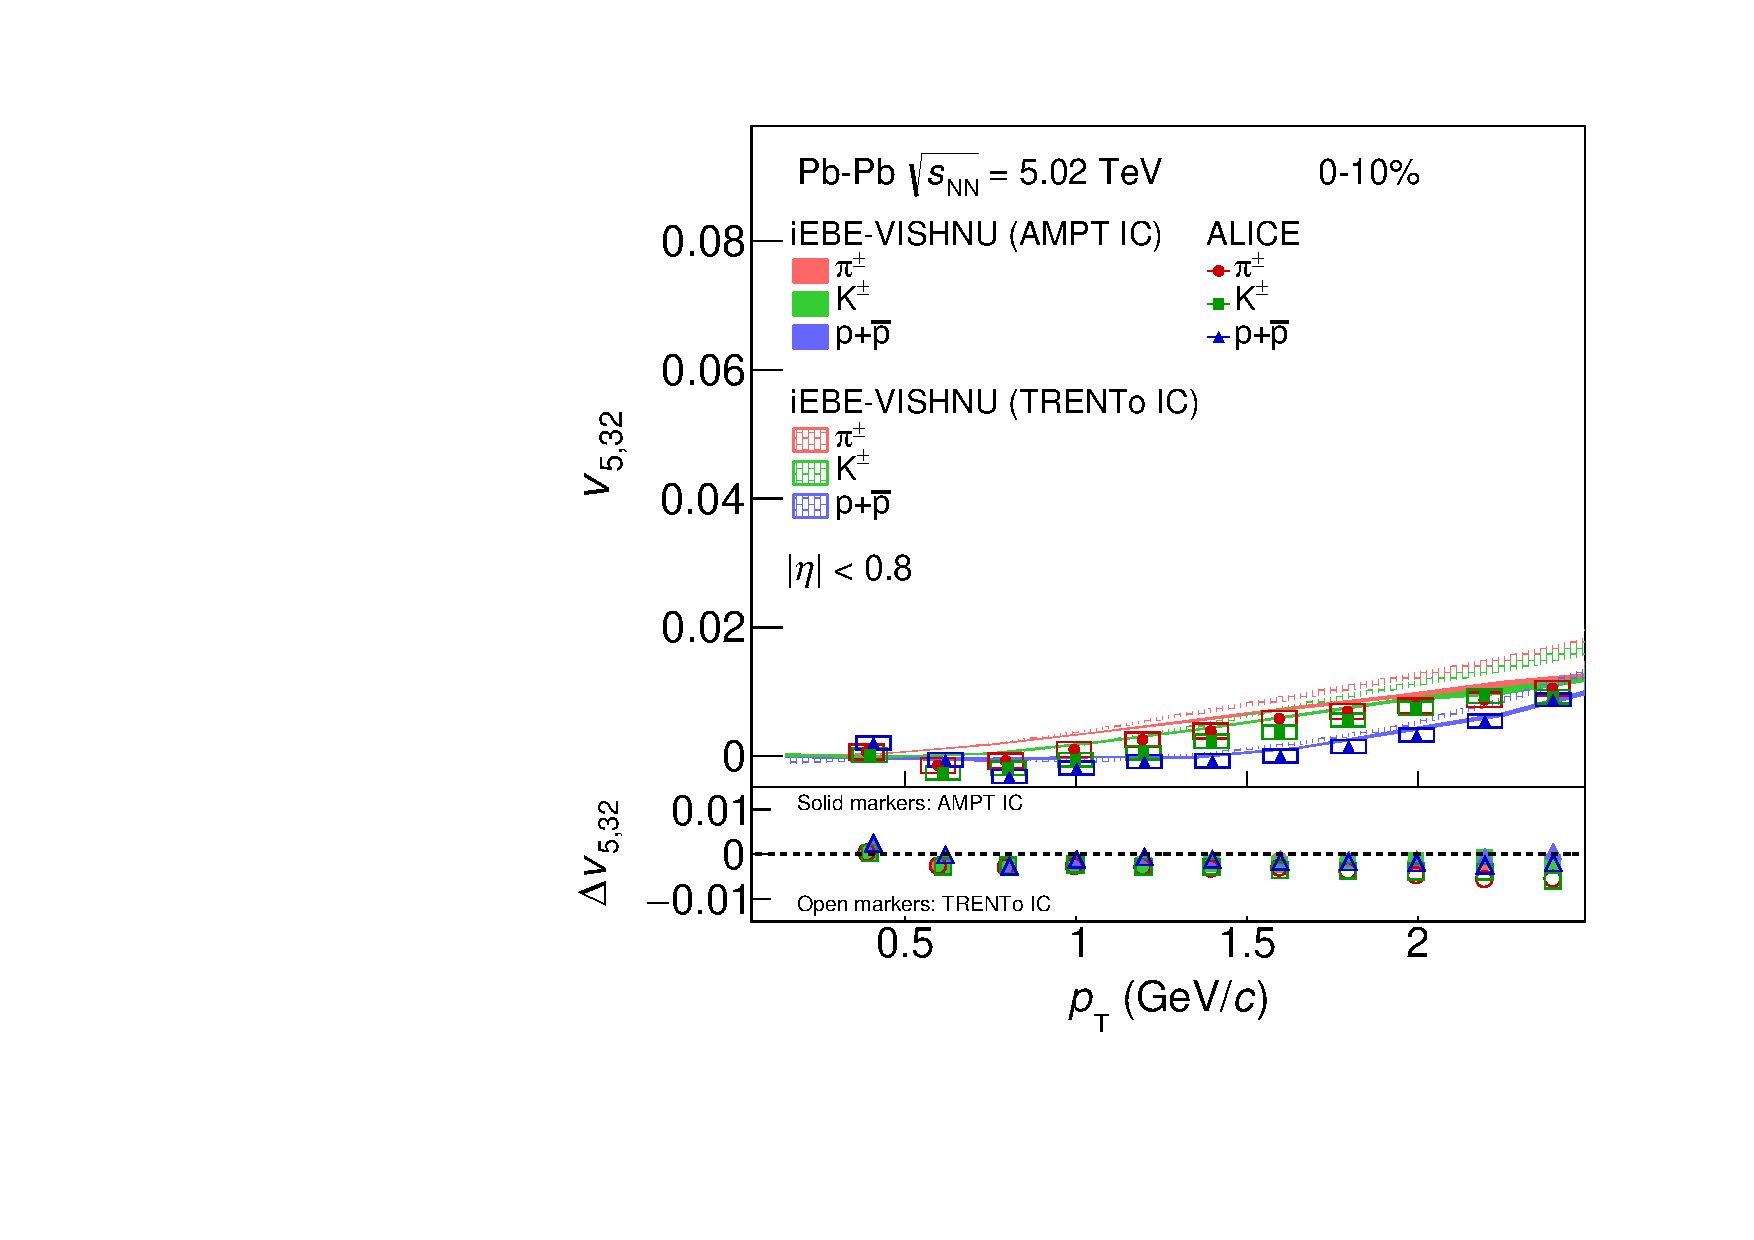
\includegraphics[scale=0.26]{figures/model/TrentoAndAMPT_v523_gap00_new_0-10_PID2.pdf}
%DIF > \includegraphics[scale=0.26]{figures/model/TrentoAndAMPT_v523_gap00_new_10-20_PID2.pdf}
%DIF > \includegraphics[scale=0.26]{figures/model/TrentoAndAMPT_v523_gap00_new_20-30_PID2.pdf}
%DIF > \includegraphics[scale=0.26]{figures/model/TrentoAndAMPT_v523_gap00_new_30-40_PID2.pdf}
%DIF > \includegraphics[scale=0.26]{figures/model/TrentoAndAMPT_v523_gap00_new_40-50_PID2.pdf}
%DIF > \includegraphics[scale=0.26]{figures/model/TrentoAndAMPT_v523_gap00_new_50-60_PID2.pdf}
\DIFaddendFL \end{center}
\caption{The \pT-differential $v_{5,32}$ for different particle species in 10-20\% up to 50-60\% centrality intervals of Pb--Pb collisions at \sNN compared with iEBE-VISHNU hybrid models with two different sets of initial parameters: AMPT initial conditions ($\eta/s$= 0.08 and $\zeta/s$ = 0) shown in solid bands and TRENTo initial conditions ($\eta/s({\rm T})$ and $\zeta/s({\rm T})$) in hatched bands. The bottom panels show the difference between the measurements and each model.}
\label{v523_model}
\end{figure}

\begin{figure}[!htb]
\begin{center}
\DIFdelbeginFL %DIFDELCMD < \includegraphics[scale=0.26]{figures/model/TrentoAndAMPT_v633_gap00_new_0-10_PID2.pdf}
%DIFDELCMD < \includegraphics[scale=0.26]{figures/model/TrentoAndAMPT_v633_gap00_new_10-20_PID2.pdf}
%DIFDELCMD < \includegraphics[scale=0.26]{figures/model/TrentoAndAMPT_v633_gap00_new_20-30_PID2.pdf}
%DIFDELCMD < \includegraphics[scale=0.26]{figures/model/TrentoAndAMPT_v633_gap00_new_30-40_PID2.pdf}
%DIFDELCMD < \includegraphics[scale=0.26]{figures/model/TrentoAndAMPT_v633_gap00_new_40-50_PID2.pdf}
%DIFDELCMD < %%%
\DIFdelendFL \DIFaddbeginFL \includegraphics[scale=0.73]{figures/model/TrentoAndAMPT_v633_gap00_PID2.pdf}
%DIF > \includegraphics[scale=0.26]{figures/model/TrentoAndAMPT_v633_gap00_new_0-10_PID2.pdf}
%DIF > \includegraphics[scale=0.26]{figures/model/TrentoAndAMPT_v633_gap00_new_10-20_PID2.pdf}
%DIF > \includegraphics[scale=0.26]{figures/model/TrentoAndAMPT_v633_gap00_new_20-30_PID2.pdf}
%DIF > \includegraphics[scale=0.26]{figures/model/TrentoAndAMPT_v633_gap00_new_30-40_PID2.pdf}
%DIF > \includegraphics[scale=0.26]{figures/model/TrentoAndAMPT_v633_gap00_new_40-50_PID2.pdf}
\DIFaddendFL \end{center}
\caption{The \pT-differential $v_{6,33}$ for different particle species in 10-20\% up to 40-50\% centrality intervals of Pb--Pb collisions at \sNN compared with iEBE-VISHNU hybrid models with two different sets of initial parameters: AMPT initial conditions ($\eta/s$= 0.08 and $\zeta/s$ = 0) shown in solid bands and TRENTo initial conditions ($\eta/s({\rm T})$ and $\zeta/s({\rm T})$) in hatched bands. The bottom panels show the difference between the measurements and each model.}
\label{v633_model}
\end{figure}


\begin{figure}[!htb]
\begin{center}
\DIFdelbeginFL %DIFDELCMD < \includegraphics[scale=0.26]{figures/model/TrentoAndAMPT_v6222_gap00_new_0-10_PID2.pdf}
%DIFDELCMD < \includegraphics[scale=0.26]{figures/model/TrentoAndAMPT_v6222_gap00_new_10-20_PID2.pdf}
%DIFDELCMD < \includegraphics[scale=0.26]{figures/model/TrentoAndAMPT_v6222_gap00_new_20-30_PID2.pdf}
%DIFDELCMD < \includegraphics[scale=0.26]{figures/model/TrentoAndAMPT_v6222_gap00_new_30-40_PID2.pdf}
%DIFDELCMD < \includegraphics[scale=0.26]{figures/model/TrentoAndAMPT_v6222_gap00_new_40-50_PID2.pdf}
%DIFDELCMD < \includegraphics[scale=0.26]{figures/model/TrentoAndAMPT_v6222_gap00_new_50-60_PID2.pdf}
%DIFDELCMD < %%%
\DIFdelendFL \DIFaddbeginFL \includegraphics[scale=0.73]{figures/model/TrentoAndAMPT_v6222_gap00_PID2.pdf}
%DIF > \includegraphics[scale=0.26]{figures/model/TrentoAndAMPT_v6222_gap00_new_0-10_PID2.pdf}
%DIF > \includegraphics[scale=0.26]{figures/model/TrentoAndAMPT_v6222_gap00_new_10-20_PID2.pdf}
%DIF > \includegraphics[scale=0.26]{figures/model/TrentoAndAMPT_v6222_gap00_new_20-30_PID2.pdf}
%DIF > \includegraphics[scale=0.26]{figures/model/TrentoAndAMPT_v6222_gap00_new_30-40_PID2.pdf}
%DIF > \includegraphics[scale=0.26]{figures/model/TrentoAndAMPT_v6222_gap00_new_40-50_PID2.pdf}
%DIF > \includegraphics[scale=0.26]{figures/model/TrentoAndAMPT_v6222_gap00_new_50-60_PID2.pdf}
\DIFaddendFL \end{center}
\caption{The \pT-differential $v_{6,222}$ for different particle species in 10-20\% up to 50-60\% centrality intervals of Pb--Pb collisions at \sNN compared with iEBE-VISHNU hybrid models with two different sets of initial parameters: AMPT initial conditions ($\eta/s$= 0.08 and $\zeta/s$ = 0) shown in solid bands and TRENTo initial conditions ($\eta/s({\rm T})$ and $\zeta/s({\rm T})$) in hatched bands. The bottom panels show the difference between the measurements and each model.}
\label{v6222_model}
\end{figure}



\newpage
\newpage

\section{Summary}
\label{Sec:conclusion}

In this article, a measurement of non-linear flow modes, $v_{4,22}$, $v_{5,32}$, $v_{6,222}$ and $v_{6,33}$ as a function of transverse momentum for different particle species, i.e. \pion, \kaon, \proton, \Ks, \lambdas~and $\phi$-meson are reported for a wide range of centrality intervals from 0-5\% up to 50-60\% in Pb--Pb collisions at \sNN. The non-linear flow modes, $v_{n,mk}$, are calculated with a multi-particle correlation technique, namely the generic framework, selecting the identified hadron under study and the reference flow particles from different, non-overlapping pseudorapidity regions. This multi-particle correlation technique by nature removes majority of non-flow correlations. In order to reduce non-flow contributions further, a non-zero gap was applied between the two pseudorapidity regions as well as selecting like sign particles of interest and reference particles. These variations did not affect the results significantly but any variation was included in the final systematics. 

The magnitude of $v_{4,22}$, $v_{5,32}$ and $v_{6,222}$ exhibit a clear centrality dependence. This centrality dependence originates from the contribution of second order flow harmonic, as shown in Eq. \ref{Eq:V4V5V6}, and reflects the dependence of $v_{2}$ on the anisotropy of the collision geometry. As expected, $v_{6,33}$ does not exhibit a considerable centrality dependence since $v_{3}$ is primarily generated by event-by-event fluctuations of the initial energy density profile. This is supported by the relatively large magnitude of $v_{6,33}$ in the most-central collisions (0-5\%). A clear mass ordering is observed in the low \pT~region (\pT$< 2.5$ \GeV). This observation is associated with the interplay between the \DIFdelbegin \DIFdel{non-linear flow modes }\DIFdelend \DIFaddbegin \DIFadd{anisotropic flow }\DIFaddend and radial flow. In the intermediate \pT~region (\pT$> 2.5$ \GeV), a particle type grouping is observed where the magnitude of non-linear modes for baryons are larger than for mesons. The NCQ scaling holds at best in an approximate level of $\pm 20$\% within the current level of statistical and systematic uncertainties similar to that of total flow coefficients \cite{Acharya:2018zuq}.

The comparison of two models based on the iEBE-VISHNU hybrid model, and with two different initial conditions (AMPT and TRENTo) and transport properties show that neither of the models are able to fully describe the measurements. This varies depending on the centrality percentile. Measurements are better predicted by the models in more central collisions. All in all, the model using AMPT initial conditions ($\eta/s = 0.08$ and $\zeta/s =0$) exhibits a magnitude and shape closer to the measurements. As a result, in order to further constrain the values of transport properties and the initial conditions of the system, it is necessary to tune the input parameters of future hydrodynamic calculations attempting to describe these measurements.
%\section{Appendix}
\label{Sec:appendix}


%%%%%%%%%%%%%%%%%%%%%%%%%%%%%%%%
% end main text 
%%%%%%%%%%%%%%%%%%%%%%%%%%%%%%%%

%%%%% acknowledgements - handled by EB chairs 
\newenvironment{acknowledgement}{\relax}{\relax}
\begin{acknowledgement}
\section*{Acknowledgements}
% add specific acknowledgements here 
% ...but please don't remove the line below: funding agencies
% will be acknowledged with a custom tex file handled by EB chairs after Collab Round 2
%\input{acknowledgements.tex}
\end{acknowledgement}

\newpage

%%%%%%%% Bibliography 
\bibliographystyle{utphys}   % Remember we use title in the biblio
\providecommand{\href}[2]{#2}\begingroup\raggedright\begin{thebibliography}{10}

\bibitem{Borsanyi:2010cj}
S.~Borsanyi, G.~Endrodi, Z.~Fodor, A.~Jakovac, S.~D. Katz, S.~Krieg, C.~Ratti,
  and K.~K. Szabo, ``{The QCD equation of state with dynamical quarks}'',
  \href{http://dx.doi.org/10.1007/JHEP11(2010)077}{{\em JHEP} {\bfseries 11}
  (2010) },
\href{http://arxiv.org/abs/1007.2580}{{\ttfamily arXiv:1007.2580 [hep-lat]}}.
%%CITATION = ARXIV:1007.2580;%%.

\bibitem{Bhattacharya:2014ara}
T.~Bhattacharya {\em et~al.}, ``{QCD Phase Transition with Chiral Quarks and
  Physical Quark Masses}'',
  \href{http://dx.doi.org/10.1103/PhysRevLett.113.082001}{{\em Phys. Rev.
  Lett.} {\bfseries 113} no.~8, (2014) },
\href{http://arxiv.org/abs/1402.5175}{{\ttfamily arXiv:1402.5175 [hep-lat]}}.
%%CITATION = ARXIV:1402.5175;%%.

\bibitem{Shuryak:1984nq}
E.~V. Shuryak, ``{Theory and phenomenology of the QCD vacuum}'',
\href{http://dx.doi.org/10.1016/0370-1573(84)90037-1}{{\em Phys. Rept.}
  {\bfseries 115} (1984) }.
%%CITATION = PRPLC,115,151;%%.

\bibitem{Cleymans:1985wb}
J.~Cleymans, R.~V. Gavai, and E.~Suhonen, ``{Quarks and Gluons at High
  Temperatures and Densities}'',
\href{http://dx.doi.org/10.1016/0370-1573(86)90169-9}{{\em Phys. Rept.}
  {\bfseries 130} (1986) }.
%%CITATION = PRPLC,130,217;%%.

\bibitem{Bass:1998vz}
S.~A. Bass, M.~Gyulassy, H.~Stoecker, and W.~Greiner, ``{Signatures of quark
  gluon plasma formation in high-energy heavy ion collisions: A Critical
  review}'', \href{http://dx.doi.org/10.1088/0954-3899/25/3/013}{{\em J. Phys.}
  {\bfseries G25} (1999) },
\href{http://arxiv.org/abs/hep-ph/9810281}{{\ttfamily arXiv:hep-ph/9810281
  [hep-ph]}}.
%%CITATION = HEP-PH/9810281;%%.

\bibitem{Bhalerao:2006tp}
R.~S. Bhalerao and J.-Y. Ollitrault, ``{Eccentricity fluctuations and elliptic
  flow at RHIC}'', \href{http://dx.doi.org/10.1016/j.physletb.2006.08.055}{{\em
  Phys. Lett.} {\bfseries B641} (2006) },
\href{http://arxiv.org/abs/nucl-th/0607009}{{\ttfamily arXiv:nucl-th/0607009
  [nucl-th]}}.
%%CITATION = NUCL-TH/0607009;%%.

\bibitem{Alver:2008zza}
B.~Alver {\em et~al.}, ``{Importance of correlations and fluctuations on the
  initial source eccentricity in high-energy nucleus-nucleus collisions}'',
  \href{http://dx.doi.org/10.1103/PhysRevC.77.014906}{{\em Phys. Rev.}
  {\bfseries C77} (2008) },
\href{http://arxiv.org/abs/0711.3724}{{\ttfamily arXiv:0711.3724 [nucl-ex]}}.
%%CITATION = ARXIV:0711.3724;%%.

\bibitem{Alver:2010gr}
B.~Alver and G.~Roland, ``{Collision geometry fluctuations and triangular flow
  in heavy-ion collisions}'',
  \href{http://dx.doi.org/10.1103/PhysRevC.82.039903,
  10.1103/PhysRevC.81.054905}{{\em Phys. Rev.} {\bfseries C81} (2010) },
  \href{http://arxiv.org/abs/1003.0194}{{\ttfamily arXiv:1003.0194 [nucl-th]}}.
[Erratum: Phys. Rev.C82,039903(2010)].
%%CITATION = ARXIV:1003.0194;%%.

\bibitem{Alver:2010dn}
B.~H. Alver, C.~Gombeaud, M.~Luzum, and J.-Y. Ollitrault, ``{Triangular flow in
  hydrodynamics and transport theory}'',
  \href{http://dx.doi.org/10.1103/PhysRevC.82.034913}{{\em Phys. Rev.}
  {\bfseries C82} (2010) },
\href{http://arxiv.org/abs/1007.5469}{{\ttfamily arXiv:1007.5469 [nucl-th]}}.
%%CITATION = ARXIV:1007.5469;%%.

\bibitem{Manly:2005zy}
{\bfseries PHOBOS} Collaboration, S.~Manly {\em et~al.}, ``{System size, energy
  and pseudorapidity dependence of directed and elliptic flow at RHIC}'',
  \href{http://dx.doi.org/10.1016/j.nuclphysa.2006.06.079}{{\em Nucl. Phys.}
  {\bfseries A774} (2006) },
\href{http://arxiv.org/abs/nucl-ex/0510031}{{\ttfamily arXiv:nucl-ex/0510031
  [nucl-ex]}}.
%%CITATION = NUCL-EX/0510031;%%.

\DIFaddbegin \bibitem{Voloshin:1994mz}
\DIFadd{S.~Voloshin and Y.~Zhang, ``}{\DIFadd{Flow study in relativistic nuclear collisions by
  Fourier expansion of Azimuthal particle distributions}}\DIFadd{'',
  }\href{http://dx.doi.org/10.1007/s002880050141}{{\em Z. Phys.} {\bfseries C70}
  (1996) }\DIFadd{,
}\href{http://arxiv.org/abs/hep-ph/9407282}{{\ttfamily arXiv:hep-ph/9407282
  [hep-ph]}}\DIFadd{.
%DIF > %CITATION = HEP-PH/9407282;%%.
}

\bibitem{Poskanzer:1998yz}
\DIFadd{A.~M. Poskanzer and S.~A. Voloshin, ``}{\DIFadd{Methods for analyzing anisotropic flow
  in relativistic nuclear collisions}}\DIFadd{'',
  }\href{http://dx.doi.org/10.1103/PhysRevC.58.1671}{{\em Phys. Rev.} {\bfseries
  C58} (1998) }\DIFadd{,
}\href{http://arxiv.org/abs/nucl-ex/9805001}{{\ttfamily arXiv:nucl-ex/9805001
  [nucl-ex]}}\DIFadd{.
%DIF > %CITATION = NUCL-EX/9805001;%%.
}

\DIFaddend \bibitem{Adams:2003am}
{\bfseries STAR} Collaboration, J.~Adams {\em et~al.}, ``{Particle type
  dependence of azimuthal anisotropy and nuclear modification of particle
  production in Au + Au collisions at $\sqrt{s_{NN}} = $200~GeV}'',
  \href{http://dx.doi.org/10.1103/PhysRevLett.92.052302}{{\em Phys. Rev. Lett.}
  {\bfseries 92} (2004) },
\href{http://arxiv.org/abs/nucl-ex/0306007}{{\ttfamily arXiv:nucl-ex/0306007
  [nucl-ex]}}.
%%CITATION = NUCL-EX/0306007;%%.

\bibitem{Abelev:2007qg}
{\bfseries STAR} Collaboration, B.~I. Abelev {\em et~al.}, ``{Mass,
  quark-number, and $\sqrt{s_{NN}}$ dependence of the second and fourth flow
  harmonics in ultra-relativistic nucleus-nucleus collisions}'',
  \href{http://dx.doi.org/10.1103/PhysRevC.75.054906}{{\em Phys. Rev.}
  {\bfseries C75} (2007) },
\href{http://arxiv.org/abs/nucl-ex/0701010}{{\ttfamily arXiv:nucl-ex/0701010
  [nucl-ex]}}.
%%CITATION = NUCL-EX/0701010;%%.

\bibitem{Adler:2003kt}
{\bfseries PHENIX} Collaboration, S.~S. Adler {\em et~al.}, ``{Elliptic flow of
  identified hadrons in Au+Au collisions at $\sqrt{s_{NN}} = $200~GeV}'',
  \href{http://dx.doi.org/10.1103/PhysRevLett.91.182301}{{\em Phys. Rev. Lett.}
  {\bfseries 91} (2003) },
\href{http://arxiv.org/abs/nucl-ex/0305013}{{\ttfamily arXiv:nucl-ex/0305013
  [nucl-ex]}}.
%%CITATION = NUCL-EX/0305013;%%.

\bibitem{Adare:2006ti}
{\bfseries PHENIX} Collaboration, A.~Adare {\em et~al.}, ``{Scaling properties
  of azimuthal anisotropy in Au+Au and Cu+Cu collisions at s(NN) = 200-GeV}'',
  \href{http://dx.doi.org/10.1103/PhysRevLett.98.162301}{{\em Phys. Rev. Lett.}
  {\bfseries 98} (2007) },
\href{http://arxiv.org/abs/nucl-ex/0608033}{{\ttfamily arXiv:nucl-ex/0608033
  [nucl-ex]}}.
%%CITATION = NUCL-EX/0608033;%%.

\bibitem{Abelev:2014pua}
{\bfseries ALICE} Collaboration, B.~B. Abelev {\em et~al.}, ``{Elliptic flow of
  identified hadrons in Pb-Pb collisions at $ \sqrt{s_{\mathrm{NN}}}=2.76 $
  TeV}'', \href{http://dx.doi.org/10.1007/JHEP06(2015)190}{{\em JHEP}
  {\bfseries 06} (2015) },
\href{http://arxiv.org/abs/1405.4632}{{\ttfamily arXiv:1405.4632 [nucl-ex]}}.
%%CITATION = ARXIV:1405.4632;%%.

\bibitem{Adam:2016nfo}
{\bfseries ALICE} Collaboration, J.~Adam {\em et~al.}, ``{Higher harmonic flow
  coefficients of identified hadrons in Pb-Pb collisions at $\sqrt{s_{\rm NN}}$
  = 2.76 TeV}'', \href{http://dx.doi.org/10.1007/JHEP09(2016)164}{{\em JHEP}
  {\bfseries 09} (2016) },
\href{http://arxiv.org/abs/1606.06057}{{\ttfamily arXiv:1606.06057 [nucl-ex]}}.
%%CITATION = ARXIV:1606.06057;%%.

\bibitem{Acharya:2018zuq}
{\bfseries ALICE} Collaboration, S.~Acharya {\em et~al.}, ``{Anisotropic flow
  of identified particles in Pb-Pb collisions at $
  {\sqrt{s}}_{\mathrm{NN}}=5.02 $ TeV}'',
  \href{http://dx.doi.org/10.1007/JHEP09(2018)006}{{\em JHEP} {\bfseries 09}
  (2018) },
\href{http://arxiv.org/abs/1805.04390}{{\ttfamily arXiv:1805.04390 [nucl-ex]}}.
%%CITATION = ARXIV:1805.04390;%%.

\bibitem{Kovtun:2004de}
P.~Kovtun, D.~T. Son, and A.~O. Starinets, ``{Viscosity in strongly interacting
  quantum field theories from black hole physics}'',
  \href{http://dx.doi.org/10.1103/PhysRevLett.94.111601}{{\em Phys. Rev. Lett.}
  {\bfseries 94} (2005) },
\href{http://arxiv.org/abs/hep-th/0405231}{{\ttfamily arXiv:hep-th/0405231
  [hep-th]}}.
%%CITATION = HEP-TH/0405231;%%.

\bibitem{Adam:2016izf}
{\bfseries ALICE} Collaboration, J.~Adam {\em et~al.}, ``{Anisotropic flow of
  charged particles in Pb-Pb collisions at $\sqrt{s_{\rm NN}}=5.02$ TeV}'',
  \href{http://dx.doi.org/10.1103/PhysRevLett.116.132302}{{\em Phys. Rev.
  Lett.} {\bfseries 116} no.~13, (2016) },
\href{http://arxiv.org/abs/1602.01119}{{\ttfamily arXiv:1602.01119 [nucl-ex]}}.
%%CITATION = ARXIV:1602.01119;%%.

\DIFdelbegin %DIFDELCMD < \bibitem{Bhalerao:2014xra}
%DIFDELCMD < %%%
\DIFdel{R.~S. Bhalerao, J.-Y. Ollitrault, and S.~Pal}\DIFdelend \DIFaddbegin \bibitem{Teaney:2010vd}
\DIFadd{D.~Teaney and L.~Yan}\DIFaddend , ``{\DIFdelbegin \DIFdel{Characterizing flow
  fluctuations with moments}\DIFdelend \DIFaddbegin \DIFadd{Triangularity and Dipole Asymmetry in Heavy Ion
  Collisions}\DIFaddend }'', \DIFdelbegin %DIFDELCMD < \href{http://dx.doi.org/10.1016/j.physletb.2015.01.019}{{\em Phys. Lett.}
%DIFDELCMD <   {\bfseries B742} (2015) }%%%
\DIFdel{,
}%DIFDELCMD < \href{http://arxiv.org/abs/1411.5160}{{\ttfamily arXiv:1411.5160 [nucl-th]}}%%%
\DIFdel{.
%DIF < %CITATION = ARXIV:1411.5160;%%.
}\DIFdelend \DIFaddbegin \href{http://dx.doi.org/10.1103/PhysRevC.83.064904}{{\em Phys.
  Rev.} {\bfseries C83} (2011) }\DIFadd{,
}\href{http://arxiv.org/abs/1010.1876}{{\ttfamily arXiv:1010.1876 [nucl-th]}}\DIFadd{.
%DIF > %CITATION = ARXIV:1010.1876;%%.
}\DIFaddend 

\bibitem{Teaney:2013dta}
D.~Teaney and L.~Yan, ``{Event-plane correlations and hydrodynamic simulations
  of heavy ion collisions}'',
  \href{http://dx.doi.org/10.1103/PhysRevC.90.024902}{{\em Phys. Rev.}
  {\bfseries C90} no.~2, (2014) },
\href{http://arxiv.org/abs/1312.3689}{{\ttfamily arXiv:1312.3689 [nucl-th]}}.
%%CITATION = ARXIV:1312.3689;%%.

\DIFaddbegin \bibitem{Bhalerao:2014xra}
\DIFadd{R.~S. Bhalerao, J.-Y. Ollitrault, and S.~Pal, ``}{\DIFadd{Characterizing flow
  fluctuations with moments}}\DIFadd{'',
  }\href{http://dx.doi.org/10.1016/j.physletb.2015.01.019}{{\em Phys. Lett.}
  {\bfseries B742} (2015) }\DIFadd{,
}\href{http://arxiv.org/abs/1411.5160}{{\ttfamily arXiv:1411.5160 [nucl-th]}}\DIFadd{.
%DIF > %CITATION = ARXIV:1411.5160;%%.
}

\DIFaddend \bibitem{Qian:2017ier}
J.~Qian, U.~Heinz, R.~He, and L.~Huo, ``{Differential flow correlations in
  relativistic heavy-ion collisions}'',
  \href{http://dx.doi.org/10.1103/PhysRevC.95.054908}{{\em Phys. Rev.}
  {\bfseries C95} no.~5, (2017) },
\href{http://arxiv.org/abs/1703.04077}{{\ttfamily arXiv:1703.04077 [nucl-th]}}.
%%CITATION = ARXIV:1703.04077;%%.

\bibitem{Yan:2015jma}
L.~Yan and J.-Y. Ollitrault, ``{$\nu_4, \nu_5, \nu_6, \nu_7$: nonlinear
  hydrodynamic response versus LHC data}'',
  \href{http://dx.doi.org/10.1016/j.physletb.2015.03.040}{{\em Phys. Lett.}
  {\bfseries B744} (2015) },
\href{http://arxiv.org/abs/1502.02502}{{\ttfamily arXiv:1502.02502 [nucl-th]}}.
%%CITATION = ARXIV:1502.02502;%%.

\bibitem{Acharya:2017zfg}
{\bfseries ALICE} Collaboration, S.~Acharya {\em et~al.}, ``{Linear and
  non-linear flow modes in Pb-Pb collisions at $\sqrt{s_{\rm NN}} =$ 2.76
  TeV}'', \href{http://dx.doi.org/10.1016/j.physletb.2017.07.060}{{\em Phys.
  Lett.} {\bfseries B773} (2017) },
\href{http://arxiv.org/abs/1705.04377}{{\ttfamily arXiv:1705.04377 [nucl-ex]}}.
%%CITATION = ARXIV:1705.04377;%%.

\DIFaddbegin \bibitem{ALICE:2011ab}
{\bfseries \DIFadd{ALICE}} \DIFadd{Collaboration, K.~Aamodt }{\em \DIFadd{et~al.}}\DIFadd{, ``}{\DIFadd{Higher harmonic
  anisotropic flow measurements of charged particles in Pb-Pb collisions at
  $\sqrt{s_{NN}}$=2.76 TeV}}\DIFadd{'',
  }\href{http://dx.doi.org/10.1103/PhysRevLett.107.032301}{{\em Phys. Rev.
  Lett.} {\bfseries 107} (2011) }\DIFadd{,
}\href{http://arxiv.org/abs/1105.3865}{{\ttfamily arXiv:1105.3865 [nucl-ex]}}\DIFadd{.
%DIF > %CITATION = ARXIV:1105.3865;%%.
}

\bibitem{ATLAS:2012at}
{\bfseries \DIFadd{ATLAS}} \DIFadd{Collaboration, G.~Aad }{\em \DIFadd{et~al.}}\DIFadd{, ``}{\DIFadd{Measurement of the
  azimuthal anisotropy for charged particle production in $\sqrt{s_{NN}}=2.76$
  TeV lead-lead collisions with the ATLAS detector}}\DIFadd{'',
  }\href{http://dx.doi.org/10.1103/PhysRevC.86.014907}{{\em Phys. Rev.}
  {\bfseries C86} (2012) }\DIFadd{,
}\href{http://arxiv.org/abs/1203.3087}{{\ttfamily arXiv:1203.3087 [hep-ex]}}\DIFadd{.
%DIF > %CITATION = ARXIV:1203.3087;%%.
}

\bibitem{Chatrchyan:2013kba}
{\bfseries \DIFadd{CMS}} \DIFadd{Collaboration, S.~Chatrchyan }{\em \DIFadd{et~al.}}\DIFadd{, ``}{\DIFadd{Measurement of
  higher-order harmonic azimuthal anisotropy in PbPb collisions at
  $\sqrt{s_{NN}}$ = 2.76 TeV}}\DIFadd{'',
  }\href{http://dx.doi.org/10.1103/PhysRevC.89.044906}{{\em Phys. Rev.}
  {\bfseries C89} no.~4, (2014) }\DIFadd{,
}\href{http://arxiv.org/abs/1310.8651}{{\ttfamily arXiv:1310.8651 [nucl-ex]}}\DIFadd{.
%DIF > %CITATION = ARXIV:1310.8651;%%.
}

\bibitem{Acharya:2018lmh}
{\bfseries \DIFadd{ALICE}} \DIFadd{Collaboration, S.~Acharya }{\em \DIFadd{et~al.}}\DIFadd{, ``}{\DIFadd{Energy dependence
  and fluctuations of anisotropic flow in Pb-Pb collisions at $
  \sqrt{s_{\mathrm{NN}}}=5.02 $ and 2.76 TeV}}\DIFadd{'',
  }\href{http://dx.doi.org/10.1007/JHEP07(2018)103}{{\em JHEP} {\bfseries 07}
  (2018) }\DIFadd{,
}\href{http://arxiv.org/abs/1804.02944}{{\ttfamily arXiv:1804.02944 [nucl-ex]}}\DIFadd{.
%DIF > %CITATION = ARXIV:1804.02944;%%.
}

\bibitem{Voloshin:1996nv}
\DIFadd{S.~A. Voloshin, ``}{\DIFadd{Transverse radial expansion and directed flow}}\DIFadd{'',
  }\href{http://dx.doi.org/10.1103/PhysRevC.55.R1630}{{\em Phys. Rev.}
  {\bfseries C55} (1997) }\DIFadd{,
}\href{http://arxiv.org/abs/nucl-th/9611038}{{\ttfamily arXiv:nucl-th/9611038
  [nucl-th]}}\DIFadd{.
%DIF > %CITATION = NUCL-TH/9611038;%%.
}

\bibitem{Huovinen:2001cy}
\DIFadd{P.~Huovinen, P.~F. Kolb, U.~W. Heinz, P.~V. Ruuskanen, and S.~A. Voloshin,
  ``}{\DIFadd{Radial and elliptic flow at RHIC: Further predictions}}\DIFadd{'',
  }\href{http://dx.doi.org/10.1016/S0370-2693(01)00219-2}{{\em Phys. Lett.}
  {\bfseries B503} (2001) }\DIFadd{,
}\href{http://arxiv.org/abs/hep-ph/0101136}{{\ttfamily arXiv:hep-ph/0101136
  [hep-ph]}}\DIFadd{.
%DIF > %CITATION = HEP-PH/0101136;%%.
}

\DIFaddend \bibitem{Adam:2015eta}
{\bfseries ALICE} Collaboration, J.~Adam {\em et~al.}, ``{Event shape
  engineering for inclusive spectra and elliptic flow in Pb-Pb collisions at
  $\sqrt{s_{NN}} = 2.76$ TeV}'',
  \href{http://dx.doi.org/10.1103/PhysRevC.93.034916}{{\em Phys. Rev.}
  {\bfseries C93} no.~3, (2016) },
\href{http://arxiv.org/abs/1507.06194}{{\ttfamily arXiv:1507.06194 [nucl-ex]}}.
%%CITATION = ARXIV:1507.06194;%%.

\bibitem{Voloshin:2002wa}
S.~A. Voloshin, ``{Anisotropic flow}'',
  \href{http://dx.doi.org/10.1016/S0375-9474(02)01450-1}{{\em Nucl. Phys.}
  {\bfseries A715} (2003) },
\href{http://arxiv.org/abs/nucl-ex/0210014}{{\ttfamily arXiv:nucl-ex/0210014
  [nucl-ex]}}.
%%CITATION = NUCL-EX/0210014;%%.

\bibitem{Molnar:2003ff}
D.~Molnar and S.~A. Voloshin, ``{Elliptic flow at large transverse momenta from
  quark coalescence}'',
  \href{http://dx.doi.org/10.1103/PhysRevLett.91.092301}{{\em Phys. Rev. Lett.}
  {\bfseries 91} (2003) },
\href{http://arxiv.org/abs/nucl-th/0302014}{{\ttfamily arXiv:nucl-th/0302014
  [nucl-th]}}.
%%CITATION = NUCL-TH/0302014;%%.

\bibitem{Adare:2012vq}
{\bfseries PHENIX} Collaboration, A.~Adare {\em et~al.}, ``{Deviation from
  quark-number scaling of the anisotropy parameter $v_2$ of pions, kaons, and
  protons in Au+Au collisions at $\sqrt{s_{NN}} = 200$ GeV}'',
  \href{http://dx.doi.org/10.1103/PhysRevC.85.064914}{{\em Phys. Rev.}
  {\bfseries C85} (2012) },
\href{http://arxiv.org/abs/1203.2644}{{\ttfamily arXiv:1203.2644 [nucl-ex]}}.
%%CITATION = ARXIV:1203.2644;%%.

\bibitem{Aamodt:2008zz}
{\bfseries ALICE} Collaboration, K.~Aamodt {\em et~al.}, ``{The ALICE
  experiment at the CERN LHC}'',
\href{http://dx.doi.org/10.1088/1748-0221/3/08/S08002}{{\em JINST} {\bfseries
  3} (2008) }.
%%CITATION = JINST,3,S08002;%%.

\DIFdelbegin %DIFDELCMD < \bibitem{Bilandzic:2013kga}
%DIFDELCMD < %%%
\DIFdel{A.~Bilandzic, C.~H. Christensen, K.~Gulbrandsen, A.~Hansen, and Y.~Zhou,
  ``}%DIFDELCMD < {%%%
\DIFdel{Generic framework for anisotropic flow analyses with multiparticle
  azimuthal correlations}%DIFDELCMD < }%%%
\DIFdel{'',
  }%DIFDELCMD < \href{http://dx.doi.org/10.1103/PhysRevC.89.064904}{{\em Phys. Rev.}
%DIFDELCMD <   {\bfseries C89} no.~6, (2014) }%%%
\DIFdel{,
}%DIFDELCMD < \href{http://arxiv.org/abs/1312.3572}{{\ttfamily arXiv:1312.3572 [nucl-ex]}}%%%
\DIFdel{.
%DIF < %CITATION = ARXIV:1312.3572;%%.
}%DIFDELCMD < 

%DIFDELCMD < %%%
\DIFdelend \bibitem{Abelev:2014ffa}
{\bfseries ALICE} Collaboration, B.~B. Abelev {\em et~al.}, ``{Performance of
  the ALICE Experiment at the CERN LHC}'',
  \href{http://dx.doi.org/10.1142/S0217751X14300440}{{\em Int. J. Mod. Phys.}
  {\bfseries A29} (2014) },
\href{http://arxiv.org/abs/1402.4476}{{\ttfamily arXiv:1402.4476 [nucl-ex]}}.
%%CITATION = ARXIV:1402.4476;%%.

\bibitem{Aamodt:2010pb}
{\bfseries ALICE} Collaboration, K.~Aamodt {\em et~al.}, ``{Charged-particle
  multiplicity density at mid-rapidity in central Pb-Pb collisions at
  $\sqrt{s_{NN}} = 2.76$ TeV}'',
  \href{http://dx.doi.org/10.1103/PhysRevLett.105.252301}{{\em Phys. Rev.
  Lett.} {\bfseries 105} (2010) },
\href{http://arxiv.org/abs/1011.3916}{{\ttfamily arXiv:1011.3916 [nucl-ex]}}.
%%CITATION = ARXIV:1011.3916;%%.

\bibitem{Alme:2010ke}
J.~Alme {\em et~al.}, ``{The ALICE TPC, a large 3-dimensional tracking device
  with fast readout for ultra-high multiplicity events}'',
  \href{http://dx.doi.org/10.1016/j.nima.2010.04.042}{{\em Nucl. Instrum.
  Meth.} {\bfseries A622} (2010) },
\href{http://arxiv.org/abs/1001.1950}{{\ttfamily arXiv:1001.1950
  [physics.ins-det]}}.
%%CITATION = ARXIV:1001.1950;%%.

\bibitem{Abbas:2013taa}
{\bfseries ALICE} Collaboration, E.~Abbas {\em et~al.}, ``{Performance of the
  ALICE VZERO system}'',
  \href{http://dx.doi.org/10.1088/1748-0221/8/10/P10016}{{\em JINST} {\bfseries
  8} (2013) },
\href{http://arxiv.org/abs/1306.3130}{{\ttfamily arXiv:1306.3130 [nucl-ex]}}.
%%CITATION = ARXIV:1306.3130;%%.

\bibitem{Abelev:2013qoq}
{\bfseries ALICE} Collaboration, B.~Abelev {\em et~al.}, ``{Centrality
  determination of Pb-Pb collisions at $\sqrt{s_{NN}}$ = 2.76 TeV with
  ALICE}'', \href{http://dx.doi.org/10.1103/PhysRevC.88.044909}{{\em Phys.
  Rev.} {\bfseries C88} no.~4, (2013) },
\href{http://arxiv.org/abs/1301.4361}{{\ttfamily arXiv:1301.4361 [nucl-ex]}}.
%%CITATION = ARXIV:1301.4361;%%.

\bibitem{Billoir:1983mz}
P.~Billoir, ``{Track Fitting With Multiple Scattering: A New Method}'',
\href{http://dx.doi.org/10.1016/0167-5087(84)90274-6}{{\em Nucl. Instrum.
  Meth.} {\bfseries A225} (1984) }.
%%CITATION = NUIMA,A225,352;%%.

\bibitem{Billoir:1985nq}
P.~Billoir, R.~Fruhwirth, and M.~Regler, ``{TRACK ELEMENT MERGING STRATEGY AND
  VERTEX FITTING IN COMPLEX MODULAR DETECTORS}'',
\href{http://dx.doi.org/10.1016/0168-9002(85)90523-6}{{\em Nucl. Instrum.
  Meth.} {\bfseries A241} (1985) }.
%%CITATION = NUIMA,A241,115;%%.

\bibitem{Abelev:2013vea}
{\bfseries ALICE} Collaboration, B.~Abelev {\em et~al.}, ``{Centrality
  dependence of $\pi$, K, p production in Pb-Pb collisions at $\sqrt{s_{NN}}$ =
  2.76 TeV}'', \href{http://dx.doi.org/10.1103/PhysRevC.88.044910}{{\em Phys.
  Rev.} {\bfseries C88} (2013) },
\href{http://arxiv.org/abs/1303.0737}{{\ttfamily arXiv:1303.0737 [hep-ex]}}.
%%CITATION = ARXIV:1303.0737;%%.

\bibitem{Olive_2016}
K.~Olive, ``Review of particle physics'',
  \href{http://dx.doi.org/10.1088/1674-1137/40/10/100001}{{\em Chinese Physics
  C} {\bfseries 40} no.~10, (Oct, 2016) }.

\bibitem{doi:10.1080/14786440108520416}
J.~Podolanski and R.~Armenteros, ``Iii. analysis of v-events'',
  \href{http://dx.doi.org/10.1080/14786440108520416}{{\em The London,
  Edinburgh, and Dublin Philosophical Magazine and Journal of Science}
  {\bfseries 45} no.~360, (1954) }.

\DIFaddbegin \bibitem{Adam:2016acv}
{\bfseries \DIFadd{ALICE}} \DIFadd{Collaboration, J.~Adam }{\em \DIFadd{et~al.}}\DIFadd{, ``}{\DIFadd{Particle
  identification in ALICE: a Bayesian approach}}\DIFadd{'',
}\href{http://arxiv.org/abs/1602.01392}{{\ttfamily arXiv:1602.01392
  [physics.data-an]}}\DIFadd{.
%DIF > %CITATION = ARXIV:1602.01392;%%.
}

\bibitem{Bilandzic:2013kga}
\DIFadd{A.~Bilandzic, C.~H. Christensen, K.~Gulbrandsen, A.~Hansen, and Y.~Zhou,
  ``}{\DIFadd{Generic framework for anisotropic flow analyses with multiparticle
  azimuthal correlations}}\DIFadd{'',
  }\href{http://dx.doi.org/10.1103/PhysRevC.89.064904}{{\em Phys. Rev.}
  {\bfseries C89} no.~6, (2014) }\DIFadd{,
}\href{http://arxiv.org/abs/1312.3572}{{\ttfamily arXiv:1312.3572 [nucl-ex]}}\DIFadd{.
%DIF > %CITATION = ARXIV:1312.3572;%%.
}

\bibitem{Barlow:2002yb}
\DIFadd{R.~Barlow, ``}{\DIFadd{Systematic errors: Facts and fictions}}\DIFadd{'', in }{\em {\DIFadd{Advanced
  Statistical Techniques in Particle Physics. Proceedings, Conference, Durham,
  UK, March 18-22, 2002}}}\DIFadd{, pp.~134--144.
}\newblock \DIFadd{2002.
}\newblock \href{http://arxiv.org/abs/hep-ex/0207026}{{\ttfamily
  arXiv:hep-ex/0207026 [hep-ex]}}\DIFadd{.
}\newblock
\url{http://www.ippp.dur.ac.uk/Workshops/02/statistics/proceedings//barlow.pdf}\DIFadd{.
}\newblock
%DIF > %CITATION = HEP-EX/0207026;%%.

\bibitem{Shen:2011eg}
\DIFadd{C.~Shen, U.~Heinz, P.~Huovinen, and H.~Song, ``}{\DIFadd{Radial and elliptic flow in
  Pb+Pb collisions at the Large Hadron Collider from viscous hydrodynamic}}\DIFadd{'',
  }\href{http://dx.doi.org/10.1103/PhysRevC.84.044903}{{\em Phys. Rev.}
  {\bfseries C84} (2011) }\DIFadd{,
}\href{http://arxiv.org/abs/1105.3226}{{\ttfamily arXiv:1105.3226 [nucl-th]}}\DIFadd{.
%DIF > %CITATION = ARXIV:1105.3226;%%.
}

\DIFaddend \bibitem{Xu:2016hmp}
H.-J. Xu, Z.~Li, and H.~Song, ``{High order flow harmonics of identified
  hadrons in 2.76 A TeV Pb+Pb collisions}'',
\href{http://arxiv.org/abs/1602.02029}{{\ttfamily arXiv:1602.02029 [nucl-th]}}.
%%CITATION = ARXIV:1602.02029;%%.

\bibitem{McDonald:2016vlt}
S.~McDonald, C.~Shen, F.~Fillion-Gourdeau, S.~Jeon, and C.~Gale,
  ``{Hydrodynamic predictions for Pb+Pb collisions at 5.02 TeV}'',
  \href{http://dx.doi.org/10.1103/PhysRevC.95.064913}{{\em Phys. Rev.}
  {\bfseries C95} no.~6, (2017) },
\href{http://arxiv.org/abs/1609.02958}{{\ttfamily arXiv:1609.02958 [hep-ph]}}.
%%CITATION = ARXIV:1609.02958;%%.

\bibitem{Zhao:2017yhj}
W.~Zhao, H.-j. Xu, and H.~Song, ``{Collective flow in 2.76 A TeV and 5.02 A TeV
  Pb+Pb collisions}'',
  \href{http://dx.doi.org/10.1140/epjc/s10052-017-5186-x}{{\em Eur. Phys. J.}
  {\bfseries C77} no.~9, (2017) },
\href{http://arxiv.org/abs/1703.10792}{{\ttfamily arXiv:1703.10792 [nucl-th]}}.
%%CITATION = ARXIV:1703.10792;%%.

\bibitem{Shen:2014vra}
C.~Shen, Z.~Qiu, H.~Song, J.~Bernhard, S.~Bass, and U.~Heinz, ``{The
  iEBE-VISHNU code package for relativistic heavy-ion collisions}'',
  \href{http://dx.doi.org/10.1016/j.cpc.2015.08.039}{{\em Comput. Phys.
  Commun.} {\bfseries 199} (2016) },
\href{http://arxiv.org/abs/1409.8164}{{\ttfamily arXiv:1409.8164 [nucl-th]}}.
%%CITATION = ARXIV:1409.8164;%%.

\bibitem{Song:2010aq}
H.~Song, S.~A. Bass, and U.~Heinz, ``{Viscous QCD matter in a hybrid
  hydrodynamic+Boltzmann approach}'',
  \href{http://dx.doi.org/10.1103/PhysRevC.83.024912}{{\em Phys. Rev.}
  {\bfseries C83} (2011) },
\href{http://arxiv.org/abs/1012.0555}{{\ttfamily arXiv:1012.0555 [nucl-th]}}.
%%CITATION = ARXIV:1012.0555;%%.

\bibitem{Song:2007fn}
H.~Song and U.~W. Heinz, ``{Suppression of elliptic flow in a minimally viscous
  quark-gluon plasma}'',
  \href{http://dx.doi.org/10.1016/j.physletb.2007.11.019}{{\em Phys. Lett.}
  {\bfseries B658} (2008) },
\href{http://arxiv.org/abs/0709.0742}{{\ttfamily arXiv:0709.0742 [nucl-th]}}.
%%CITATION = ARXIV:0709.0742;%%.

\bibitem{Lin:2004en}
Z.-W. Lin, C.~M. Ko, B.-A. Li, B.~Zhang, and S.~Pal, ``{A Multi-phase transport
  model for relativistic heavy ion collisions}'',
  \href{http://dx.doi.org/10.1103/PhysRevC.72.064901}{{\em Phys. Rev.}
  {\bfseries C72} (2005) },
\href{http://arxiv.org/abs/nucl-th/0411110}{{\ttfamily arXiv:nucl-th/0411110
  [nucl-th]}}.
%%CITATION = NUCL-TH/0411110;%%.

\bibitem{Moreland:2014oya}
J.~S. Moreland, J.~E. Bernhard, and S.~A. Bass, ``{Alternative ansatz to
  wounded nucleon and binary collision scaling in high-energy nuclear
  collisions}'', \href{http://dx.doi.org/10.1103/PhysRevC.92.011901}{{\em Phys.
  Rev.} {\bfseries C92} no.~1, (2015) },
\href{http://arxiv.org/abs/1412.4708}{{\ttfamily arXiv:1412.4708 [nucl-th]}}.
%%CITATION = ARXIV:1412.4708;%%.

\DIFaddbegin \bibitem{Bernhard:2016tnd}
\DIFadd{J.~E. Bernhard, J.~S. Moreland, S.~A. Bass, J.~Liu, and U.~Heinz, ``}{\DIFadd{Applying
  Bayesian parameter estimation to relativistic heavy-ion collisions:
  simultaneous characterization of the initial state and quark-gluon plasma
  medium}}\DIFadd{'', }\href{http://dx.doi.org/10.1103/PhysRevC.94.024907}{{\em Phys.
  Rev.} {\bfseries C94} no.~2, (2016) }\DIFadd{,
}\href{http://arxiv.org/abs/1605.03954}{{\ttfamily arXiv:1605.03954 [nucl-th]}}\DIFadd{.
%DIF > %CITATION = ARXIV:1605.03954;%%.
}

\DIFaddend \end{thebibliography}\endgroup

%DIF < \input {bibliography.bib}  
%DIF > \documentclass[ALICE,manyauthors]{cernphprep}
\usepackage[comma,square,numbers,sort&compress]{natbib}
\usepackage{hyperref}
\usepackage{lineno}
\usepackage{xspace}

\usepackage[T1]{fontenc} % if needed
\usepackage{setspace}
\usepackage{capt-of}
\usepackage{epstopdf}
\usepackage{color}
\usepackage{multirow}
\usepackage{tabu}
 \usepackage[draft]{todonotes}
 \usepackage{float}

\usepackage{tabularx}
\usepackage{changepage}     
\usepackage[figuresright]{rotating}
\usepackage{graphicx} 

\newcolumntype{?}{!{\vrule width 2pt}}
\newcolumntype{@}{!{\vrule width 1.5pt}}


\linenumbers
\begin{document}
%%%%%%%%%%%%%%%%%%%%%%%%%%%%%%%%%%%%%%%%%%%%%%%%%%
% These are some new commands that may be useful 
% for paper writing in general. If other newcommands
% are needed for your specific paper, please feel 
% free to add here. 
%
% The currently available commands are organized in: 
% 1) Systems
% 2) Quantities
% 3) Energies and units
% 4) Detectors
% 5) particle species 
%%%%%%%%%%%%%%%%%%%%%%%%%%%%%%%%%%%%%%%%%%%%%%%%%%

% 1) SYSTEMS 
\newcommand{\pp}           {pp\xspace}
\newcommand{\ppbar}        {\mbox{$\mathrm {p\overline{p}}$}\xspace}
\newcommand{\XeXe}         {\mbox{Xe--Xe}\xspace}
\newcommand{\PbPb}         {\mbox{Pb--Pb}\xspace}
\newcommand{\pA}           {\mbox{pA}\xspace}
\newcommand{\pPb}          {\mbox{p--Pb}\xspace}
\newcommand{\AuAu}         {\mbox{Au--Au}\xspace}
\newcommand{\dAu}          {\mbox{d--Au}\xspace}

% 2) QUANTITIES 
\newcommand{\s}            {\ensuremath{\sqrt{s}}\xspace}
\newcommand{\snn}          {\ensuremath{\sqrt{s_{\mathrm{NN}}}}\xspace}
\newcommand{\pt}           {\ensuremath{p_{\rm T}}\xspace}
\newcommand{\meanpt}       {$\langle p_{\mathrm{T}}\rangle$\xspace}
\newcommand{\ycms}         {\ensuremath{y_{\rm CMS}}\xspace}
\newcommand{\ylab}         {\ensuremath{y_{\rm lab}}\xspace}
\newcommand{\etarange}[1]  {\mbox{$\left | \eta \right |~<~#1$}}
\newcommand{\yrange}[1]    {\mbox{$\left | y \right |~<~#1$}}
\newcommand{\dndy}         {\ensuremath{\mathrm{d}N_\mathrm{ch}/\mathrm{d}y}\xspace}
\newcommand{\dndeta}       {\ensuremath{\mathrm{d}N_\mathrm{ch}/\mathrm{d}\eta}\xspace}
\newcommand{\avdndeta}     {\ensuremath{\langle\dndeta\rangle}\xspace}
\newcommand{\dNdy}         {\ensuremath{\mathrm{d}N_\mathrm{ch}/\mathrm{d}y}\xspace}
\newcommand{\Npart}        {\ensuremath{N_\mathrm{part}}\xspace}
\newcommand{\Ncoll}        {\ensuremath{N_\mathrm{coll}}\xspace}
\newcommand{\dEdx}         {\ensuremath{\textrm{d}E/\textrm{d}x}\xspace}
\newcommand{\RpPb}         {\ensuremath{R_{\rm pPb}}\xspace}

% 3) ENERGIES, UNITS
\newcommand{\nineH}        {$\sqrt{s}~=~0.9$~Te\kern-.1emV\xspace}
\newcommand{\seven}        {$\sqrt{s}~=~7$~Te\kern-.1emV\xspace}
\newcommand{\twoH}         {$\sqrt{s}~=~0.2$~Te\kern-.1emV\xspace}
\newcommand{\twosevensix}  {$\sqrt{s}~=~2.76$~Te\kern-.1emV\xspace}
\newcommand{\five}         {$\sqrt{s}~=~5.02$~Te\kern-.1emV\xspace}
\newcommand{\twosevensixnn}{$\sqrt{s_{\mathrm{NN}}}~=~2.76$~Te\kern-.1emV\xspace}
\newcommand{\fivenn}       {$\sqrt{s_{\mathrm{NN}}}~=~5.02$~Te\kern-.1emV\xspace}
\newcommand{\LT}           {L{\'e}vy-Tsallis\xspace}
\newcommand{\GeVc}         {Ge\kern-.1emV/$c$\xspace}
\newcommand{\MeVc}         {Me\kern-.1emV/$c$\xspace}
\newcommand{\TeV}          {Te\kern-.1emV\xspace}
%\newcommand{\GeV}          {Ge\kern-.1emV\xspace}
\newcommand{\MeV}          {Me\kern-.1emV\xspace}
\newcommand{\GeVmass}      {Ge\kern-.2emV/$c^2$\xspace}
\newcommand{\MeVmass}      {Me\kern-.2emV/$c^2$\xspace}
\newcommand{\lumi}         {\ensuremath{\mathcal{L}}\xspace}

% 4) DETECTORS 
\newcommand{\ITS}          {\rm{ITS}\xspace}
\newcommand{\TOF}          {\rm{TOF}\xspace}
\newcommand{\ZDC}          {\rm{ZDC}\xspace}
\newcommand{\ZDCs}         {\rm{ZDCs}\xspace}
\newcommand{\ZNA}          {\rm{ZNA}\xspace}
\newcommand{\ZNC}          {\rm{ZNC}\xspace}
\newcommand{\SPD}          {\rm{SPD}\xspace}
\newcommand{\SDD}          {\rm{SDD}\xspace}
\newcommand{\SSD}          {\rm{SSD}\xspace}
\newcommand{\TPC}          {\rm{TPC}\xspace}
\newcommand{\TRD}          {\rm{TRD}\xspace}
\newcommand{\VZERO}        {\rm{V0}\xspace}
\newcommand{\VZEROA}       {\rm{V0A}\xspace}
\newcommand{\VZEROC}       {\rm{V0C}\xspace}
\newcommand{\Vdecay} 	   {\ensuremath{V^{0}}\xspace}

% 4) PARTICLE SPECIES 
\newcommand{\ee}           {\ensuremath{e^{+}e^{-}}} 
\newcommand{\pip}          {\ensuremath{\pi^{+}}\xspace}
\newcommand{\pim}          {\ensuremath{\pi^{-}}\xspace}
\newcommand{\kap}          {\ensuremath{\rm{K}^{+}}\xspace}
\newcommand{\kam}          {\ensuremath{\rm{K}^{-}}\xspace}
\newcommand{\pbar}         {\ensuremath{\rm\overline{p}}\xspace}
\newcommand{\kzero}        {\ensuremath{{\rm K}^{0}_{\rm{S}}}\xspace}
\newcommand{\lmb}          {\ensuremath{\Lambda}\xspace}
\newcommand{\almb}         {\ensuremath{\overline{\Lambda}}\xspace}
\newcommand{\Om}           {\ensuremath{\Omega^-}\xspace}
\newcommand{\Mo}           {\ensuremath{\overline{\Omega}^+}\xspace}
\newcommand{\X}            {\ensuremath{\Xi^-}\xspace}
\newcommand{\Ix}           {\ensuremath{\overline{\Xi}^+}\xspace}
\newcommand{\Xis}          {\ensuremath{\Xi^{\pm}}\xspace}
\newcommand{\Oms}          {\ensuremath{\Omega^{\pm}}\xspace}
\newcommand{\degree}       {\ensuremath{^{\rm o}}\xspace}

\newcommand{\vo}{$\rm{V^{0}}$}

\newcommand{\pT}{$p_{\mathrm{T}}$}

\newcommand{\pTnq}{$p_{\mathrm{T}}/n_{q}$}
\newcommand{\pTmT}{$(m_{\mathrm{T}}-m_{0})/n_{q}$}

\newcommand{\vtwo}{$v_{2}$}
\newcommand{\vthree}{$v_{3}$}
\newcommand{\vfour}{$v_{4}$}
\newcommand{\vfive}{$v_{5}$}
\newcommand{\vn}{$v_{n}$}

\newcommand{\etagap}{$|\Delta\eta|>0$}

\newcommand{\pion}{$\pi^{\pm}$}
\newcommand{\kaon}{$\rm{K}^{\pm}$}
\newcommand{\proton}{$\rm{p+\bar{p}}$}
\newcommand{\Ks}{$\rm{K^{0}_{S}}$}
\newcommand{\lambdas}{$\Lambda+\bar{\Lambda}$}

\newcommand{\GeV}{$\rm{GeV}/c$}
\newcommand{\sNN}{$\sqrt{s_{\mathrm{NN}}}=5.02$ TeV}

\newcommand{\red}[1]{{\color{red}{#1}}}

\newcommand{\minv}{$m_{\rm{inv}}$}

%%%%%%%%%%%%%%%  Title page %%%%%%%%%%%%%%%%%%%%%%%%
\begin{titlepage}
% the dates below correspond to CERN approval
% please don't touch: EB chairs will take care
\PHyear{XXXX}       % required, will be obtained from CERN
\PHnumber{XXX}      % required, will be obtained from CERN
\PHdate{Day Month}  % required, will be obtained from CERN
%%%%%%%%%%%%%%%%%%%%%%%%%%%%%%%%%%%%%%%%%%%%%%%%%%%%

%%% Put your own title + short title here:
\title{Non-linear flow modes of identified particles in Pb--Pb collisions at \sNN}
\ShortTitle{Non-linear flow modes of identified particles in Pb--Pb collisions}   % appears on left page headers

%%% Do not change the next lines
\Collaboration{ALICE Collaboration\thanks{See Appendix~\ref{app:collab} for the list of collaboration members}}
\ShortAuthor{ALICE Collaboration} % appears on right page headers, do not change

\begin{abstract}
\noindent The $p_{\mathrm{T}}$-differential non-linear flow modes, $v_{4,22}$, $v_{5,32}$, $v_{6,33}$ and $v_{6,222}$ for \pion, \kaon, \Ks, \proton, \lambdas~and $\phi$-meson have been measured for the first time at \sNN~in Pb--Pb collisions with the ALICE detector at the Large Hadron Collider. The results were obtained with a multi-particle technique, correlating the identified hadrons with reference charged particles from a different pseudorapidity region. 
These non-linear observables probe the contribution from the second and third order initial spatial anisotropy coefficients to higher flow harmonics. All the characteristic features observed in previous $p_{\mathrm{T}}$-differential anisotropic flow measurements for various particle species are also present in the non-linear flow modes, i.e. increase of magnitude with increasing centrality percentile, mass ordering at low $p_{\mathrm{T}}$ and particle type grouping in the intermediate $p_{\mathrm{T}}$ range. Hydrodynamical calculations (iEBE-VISHNU) that use different initial conditions and values of shear and bulk viscosity to entropy density ratios are confronted with the data at low transverse momenta. These calculations exhibit a better agreement with the anisotropic flow coefficients than the non-linear flow modes. These observations indicate that non-linear flow modes can provide additional discriminatory power in the study of initial conditions as well as new stringent constraints to hydrodynamical calculations.

\end{abstract}
\end{titlepage}

\setcounter{page}{2} %please do not remove this line
\tableofcontents
\newpage
\setcounter{page}{3}
%%%%%%%%%%%%%%%%%%%%%%%%%%%%%%%%
% begin main text
%%%%%%%%%%%%%%%%%%%%%%%%%%%%%%%%
\section{Introduction}
\label{Sec:Introduction}

Lattice quantum chromodynamics (QCD) calculations \cite{Borsanyi:2010cj,Bhattacharya:2014ara} suggest that at extremely high temperature and energy density a state of matter is produced in which quarks and gluons are no longer confined to hadrons. This state of matter is called quark-gluon plasma (QGP) \cite{Shuryak:1984nq, Cleymans:1985wb, Bass:1998vz}. The main goal of heavy-ion collision experiments is to study the properties of the QGP, such as the speed of the sound in this medium, the equation of state and its transport properties, e.g. shear and bulk viscosity.

One of the observables sensitive to the properties of the QGP is the azimuthal angular distribution of particles emitted in the plane perpendicular to the beam axis. In a heavy ion collision, the overlap region of the colliding nuclei exhibits an irregular shape \cite{Bhalerao:2006tp, Alver:2008zza, Alver:2010gr, Alver:2010dn, Manly:2005zy}. This spatial irregularity is a superposition of the geometry, i.e. centrality of the collision, and the anisotropic initial density profile of nucleons participating in the collision. Through interactions between partons and at later stages between the produced particles, this spatial irregularity is transferred into the anisotropy in momentum space which is usually expressed by the Fourier expansion of the azimuthal particle distribution according to

\begin{equation}
E\frac{\mathrm{d}^3N}{\mathrm{d}p^3} = \frac{1}{2\pi}\frac{\mathrm{d}^2N}{p_{\mathrm{T}}\mathrm{d}p_{\mathrm{T}}\mathrm{d}\eta} \Big\{1 + 2\sum_{n=1}^{\infty} v_n(p_{\mathrm{T}},\eta) \cos[n(\varphi - \Psi_n)]\Big\},
\label{Eq:Fourier}
\end{equation}

\noindent where $E$, $N$, $p$, $p_{\mathrm{T}}$, $\varphi$ and $\eta$ are the energy, particle yield, total momentum, transverse momentum, azimuthal angle and pseudorapidity of particles, respectively, and $\Psi_n$ is the azimuthal angle of the symmetry plane of the $n^{\mathrm{th}}$-order coefficient~\cite{Bhalerao:2006tp,Alver:2008zza,Alver:2010gr,Alver:2010dn}. The parameter $v_{n}$ is the magnitude of the $n^{\mathrm{th}}$-order complex flow coefficient $V_n$, defined as $V_{n} = v_{n}e^{in\Psi_n}$, and can be calculated according to 

\begin{equation}
v_{n} = \langle{\cos[n(\varphi - \Psi_n)]}\rangle,
\label{Eq:vn}
\end{equation}

where the brackets denote an average over all particles in all events. Since the symmetry planes are not accessible experimentally, the flow coefficients are estimated solely from the azimuthal angles of the particles emitted in the transverse plane. Measurements of different anisotropic flow coefficients at both RHIC \cite{Adams:2003am,Abelev:2007qg,Adler:2003kt,Adare:2006ti} and the LHC \cite{Abelev:2014pua,Adam:2016nfo,Acharya:2018zuq} have not only confirmed the production of a strongly coupled quark gluon plasma (sQGP) but they have also constrained the value of shear viscosity over entropy density ($\eta/s$) very close to the conjectured lower limit of $1/4\pi$ from AdS/CFT \cite{Kovtun:2004de}. In addition, both viscous hydrodynamical calculations and measurements \cite{Adam:2016izf} show that higher order flow coefficients and more importantly their transverse momentum dependence are more sensitive probes than lower order coefficients, i.e. \vtwo~and \vthree, of the initial spatial irregularity and its fluctuations.\\ % since higher order flow coefficients, originating from fluctuations of the initial state, probe smaller spatial scales.
%The non-vanishing higher order flow coefficients, $v_n (n>2)$, are believed to originate mainly from the fluctuations in the initial energy density profile of the colliding nucleons \cite{}. Thus, higher order flow coefficients are better probes to to understand the initial density profile of the 
The initial state spatial irregularity can be quantified with the standard (moment-based) anisotropy coefficients, $\epsilon_{n}$. Together with their corresponding initial symmetry planes, $\Phi_n$, the initial anisotropy coefficients can be calculated from the transverse positions of the participating nucleons as \cite{Alver:2010gr,Alver:2010dn} 

\begin{equation}
\epsilon_{n}e^{in\Phi_n} = \frac{\langle{r^{n}e^{in\phi}}\rangle}{\langle r^n\rangle}  (\rm{for}~n>1),
\label{Eq:epsilonn}
\end{equation}

where the brackets denote the average over the transverse position of all participating nucleons, $\phi$ is azimuthal angle and $r$ the polar distance. Model calculations show that $V_2$ and to a large extent, $V_3$ are  determined by their corresponding initial spatial anisotropy coefficients, $\epsilon_{2}$ and $\epsilon_{3}$, respectively \cite{Alver:2010gr}. It has been recently realised that $V_n~(n > 3)$ are not linearly correlated with their corresponding $\epsilon_{n}$ \cite{Bhalerao:2014xra}. In fact, a cumulant-based definition of initial anisotropic coefficient suggests additional terms in the definition of $\epsilon_{n}$ for higher order flow coefficients ($n>3$). As an example, the fourth order spatial anisotropy is given by \cite{Teaney:2013dta,Qian:2017ier} 
 
\begin{equation}
\epsilon_{4}'e^{i4\Phi'_4} = \epsilon_{4}e^{i4\Phi_4}  + \frac{3\langle{r^{2}}\rangle^{2}}{\langle r^4\rangle}\epsilon_{2}^{2}e^{i4\Phi_2}. 
\label{Eq:epsilonnprime}
\end{equation}

This dependence on lower order initial anisotropies gives rise to additional terms in the higher order flow coefficients. As a result, $V_n~(n > 3)$ obtain contributions not only from the linear response of the system to $\epsilon_{n}$, but also non-linear response proportional to the product of lower order initial spatial anisotropies \cite{Bhalerao:2014xra,Yan:2015jma}. 

It was shown in \cite{Acharya:2017zfg} that in a single event, $V_n$ with $n=4,5,6$ are decomposed to the linear ($V_{n}^{\mathrm{L}} $) and non-linear ($ V_{n}^{\mathrm{NL}}$) modes according to

\vspace{-0.55cm}
\begin{align}
V_{4} &= V_{4}^{\mathrm{L}} + V_{4}^{\mathrm{NL}} = V_{4}^{\mathrm{L}} + \chi_{4,22}(V_{2})^2, \nonumber \\
V_{5} &= V_{5}^{\mathrm{L}} + V_{5}^{\mathrm{NL}} = V_{5}^{\mathrm{L}} + \chi_{5,32}V_{3}V_{2}, \nonumber \\
V_{6} &= V_{6}^{\mathrm{L}} + V_{6}^{\mathrm{NL}} = V_{6}^{\mathrm{L}} + \chi_{6,222}(V_{2})^3 + \chi_{6,33}(V_{3})^2 + \chi_{6,42}V_{2}V_{4}^{\mathrm{L}},
\label{Eq:V4V5V6}
\end{align}
\vspace{-0.55cm}

where $\chi_{n,mk}$, known as non-linear flow mode coefficients, quantify the contributions of the non-linear modes to the total $V_{n}$ \cite{Acharya:2017zfg}.  
 
 Various measurements of total flow coefficients at the LHC \cite{Abelev:2014pua,Adam:2015eta,Adam:2016nfo,Acharya:2018zuq} and RHIC \cite{Adams:2003am,Abelev:2007qg,Adler:2003kt,Adare:2006ti} as a function of transverse momentum for different particle species have revealed that an interplay between radial flow and the total flow coefficients leads to a characteristic mass dependence in the low $p_{\rm{T}}$ region ($p_{\rm{T}} < 3~{\rm GeV}/c$). For higher values of $p_{\rm{T}}$ (up to $6~{\rm GeV}/c$) results for all total flow coefficients indicate a particle type grouping where baryons have a larger magnitude than the one of mesons. This feature was explained in a dynamical model where flow develops at the partonic level followed by quark coalescence into hadrons \cite{Voloshin:2002wa,Molnar:2003ff}. This model assumes that the invariant spectrum of produced particles is proportional to the product of the spectra of their constituents and in turn flow of produced particles is a sum of the flow of its constituents. Previous measurements of lower order total flow coefficients exhibit number of constituent quarks (NCQ) scaling at RHIC \cite{Adare:2012vq} and the LHC \cite{Abelev:2014pua,Adam:2016nfo} at an approximate level of $\pm20$\% for $p_{\rm{T}} > 3$ \GeV.

The measurements of non-linear flow modes in different collision geometries challenge hydrodynamic models to further constrain both the initial conditions of the collision system and its transport properties \cite{Acharya:2017zfg}. The \pT-dependent non-linear flow modes of identified particles are important observable for studying the characteristics of QGP. They not only put a stringent constraint on both the initial conditions of the collision system and its transport properties, i.e. $\eta/s$ and $\zeta/s$, but also allow to test the effect of late-stage interactions in the hadronic rescattering phase as well as the effect of particle production via coalescence mechanism to the development of the mass ordering and particle type grouping.

In this article, we report the first results of the $p_{\rm{T}}$-differential non-linear flow modes, $v_{4,22}$, $v_{5,32}$, $v_{6,33}$ and $v_{6,222}$ for \pion, \kaon, \proton, \Ks, \lambdas~and $\varphi$ measured in Pb--Pb collisions at the centre of mass energy per nucleon pair \sNN~with the ALICE detector \cite{Aamodt:2008zz} at the LHC. The detectors and the selection criteria used in  this analysis are described in Sec. \ref{Sec:ExpSetup} and \ref{Sec:EventTrackIdentification}, respectively. %The charged particles are identified using signals from both the Time Projection Chamber (TPC) and the Time Of Flight (TOF) detectors described in Section \ref{Sec:ExpSetup} with the procedures in Section \ref{SubSec:Identification} and neutral particles on a statistical basis using an invariant mass technique, also described in Section \ref{SubSec:Identification}. 
The results are obtained with a generic framework described in Section \ref{Sec:Analysis method} and in detail in \cite{Bilandzic:2013kga}. In this article, the identified hadron under study and the charged reference particles are obtained from different, non-overlapping pseudorapidity regions. The correlations not related to the common symmetry plane (non-flow), like those arising from jets, resonance decays and quantum statistics correlations, are suppressed by using multi-particle correlations as explained in Section \ref{Sec:Analysis method} and the residual effect is assigned as a systematic uncertainty, described in Section \ref{Sec:Systematics}. All coefficients for charged particles were measured separately for particles and anti-particles and were found to be compatible within statistical uncertainties. The reported measurements are therefore an average of the results for the opposite charges. The results are reported within the pseudorapidity range $|\eta|<0.8$ at different collision centralities between 0--60\% range of Pb--Pb collisions. 






\section{Experimental setup}
\label{Sec:ExpSetup}
ALICE~\cite{Aamodt:2008zz,Abelev:2014ffa} is one of the four large experiments at the LHC, particularly designed to cope with the large charged-particle densities present in central Pb--Pb collisions~\cite{Aamodt:2010pb}. By convention, the $z$-axis is parallel to the beam direction, the $x$-axis is horizontal and points towards the centre of the LHC, and the $y$-axis is vertical and points upwards. The apparatus consists of a set of detectors located in the central barrel, positioned inside a solenoidal magnet which generates a $0.5$~T field parallel to the beam direction, and a set of forward detectors. 

The Inner Tracking System (\ITS)~\cite{Aamodt:2008zz} and the \TPC~\cite{Alme:2010ke} are the main tracking detectors of the central barrel. The \ITS~consists of six layers of silicon detectors employing three different technologies. The two innermost layers, positioned at $r = 3.9$~cm and 7.6~cm,  are Silicon Pixel Detectors (\SPD), followed by two layers of Silicon Drift Detectors (\SDD) ($r = 15$~cm and 23.9~cm). Finally, the two outermost layers are double-sided Silicon Strip Detectors (\SSD) at $r = 38$~cm and 43~cm. The \TPC~has a cylindrical shape with an inner radius of about 85 cm, an outer radius of about 250 cm, and a length of 500 cm and it is positioned around the \ITS. It provides full azimuthal coverage in the pseudorapidity range $|\eta| < 0.9$. 

Charged particles were identified using the information from the \TPC~and the \TOF~detectors~\cite{Aamodt:2008zz}. The \TPC~allows for a simultaneous measurement of the momentum of a particle and its specific energy loss $\langle \mathrm{d}E/\mathrm{d}x \rangle$ in the gas. The detector provides a separation more than 2 standard deviations for the hadron species at $p_{\mathrm{T}} < 0.7$~GeV/$c$ and the possibility to identify particles on a statistical basis in the relativistic rise region of $\mathrm{d}E/\mathrm{d}x$ (i.e.~$2 < p_{\rm{T}} < 20$~GeV/$c$)~\cite{Abelev:2014ffa}. The $\mathrm{d}E/\mathrm{d}x$ resolution for the 5$\%$ most central Pb--Pb collisions is 6.5$\%$ and improves for more peripheral collisions. The \TOF~detector is situated at a radial distance of 3.7 m from the beam axis, around the \TPC~and provides a $3\sigma$ separation between $\pi$--K and K--$\rm{p}$ up to $p_{\mathrm{T}} = $ 2.5~GeV/$c$ and $p_{\mathrm{T}} = 4$~GeV/$c$, respectively~\cite{Abelev:2014ffa}. This is done by measuring the flight time of particles from the collision point with a resolution of about $80$~ps. The start time for the \TOF~measurement is provided by the T0 detectors, two arrays of Cherenkov counters positioned at opposite sides of the interaction points covering $4.6 < \eta < 4.9$ (T0A) and $-3.3 < \eta < -3.0$ (T0C). The start time is also determined using a combinatorial algorithm that compares the timestamps of particle hits measured by the TOF to the expected times of the tracks, assuming a common event time $t_{ev}$ \cite{Abelev:2014ffa}. Both methods of estimating the start time are fully efficient for the 50$\%$ most central Pb--Pb collisions.

A set of forward detectors, the \VZERO~scintillator arrays~\cite{Abbas:2013taa}, were used in the trigger logic and for the determination of the collision centrality. The \VZERO~consists of two detectors, the \VZEROA~and the \VZEROC, that are positioned on each side of the interaction point and cover the pseudorapidity ranges of $2.8 < \eta < 5.1$ and $-3.7 < \eta < -1.7$, respectively. 

For more details on the ALICE apparatus and the performance of the detectors, see Refs.~\cite{Aamodt:2008zz,Abelev:2014ffa}.

%\newpage
\section{Event sample, track selection and particle identification}
\label{Sec:EventTrackIdentification}
\subsection{Trigger selection and data sample}
\label{SubSec:Event}
The analysis is performed on minimum bias Pb--Pb collision data at \sNN~collected by the ALICE detector in 2015. These events were triggered by the coincidence between signals from both V0A and V0C detectors. An offline event selection, exploiting the signal arrival time in V0A and V0C, measured with a 1 ns resolution, was used to discriminate beam induced-background (e.g. beam-gas events) from collision events. This led to a reduction of background events in the analysed samples to a negligible fraction (< 0.1\%) \cite{Abelev:2014ffa}. Events with multiple reconstructed vertices were rejected by comparing multiplicity estimates from the V0 detector to those from the tracking detectors at midrapidity, exploiting the difference in readout times between the systems. The fraction of pileup events left after applying these dedicated pileup removal criteria is negligible. All events selected for the analysis had a reconstructed primary vertex position along the beam axis ($z_{vtx}$) within 10 cm from the nominal interaction point. After all the selection criteria, a filtered data sample of approximately 40 million Pb--Pb events in the 0--60\% centrality interval was analysed to produce the results presented in this article.

Events were classified according to fractions of the inelastic hadronic cross section. The 0--5\% interval represents the most central interactions (i.e. smallest impact parameter) and is referred to as most central collisions. On the other hand, the 50--60\% centrality interval corresponds to the most peripheral (i.e. largest impact parameter) collisions in the analysed sample. The centrality of the collision was estimated using the signal amplitude measured in the V0 detectors which is related to the number of particles crossing their sensitive areas. Details about the centrality determination can be found in \cite{Abelev:2013qoq}.

\subsection{Selection of primary \pion, \kaon~and \proton}
\label{SubSec:Track}
In this analysis, tracks are reconstructed using the information from the TPC and the ITS detectors. The tracking algorithm, based on the Kalman filter \cite{Billoir:1983mz,Billoir:1985nq}, starts from a collection of space points (referred to as clusters) inside the TPC and provides the quality of the fit by calculating its $\chi^{2}$ value. Each space point is reconstructed at one of the TPC pad rows \cite{Aamodt:2008zz}, where the deposited ionisation energy is also measured. The specific ionisation energy loss $\langle{\rm{dE}/dx}\rangle$ is estimated using a truncated mean, excluding the 40\% highest-charge clusters associated to the track. The obtained $\langle{\rm{dE}/dx}\rangle$ has a resolution, which we later refer to as $\sigma_{\rm{TPC}}$. The tracks are propagated to the outer layer of the ITS, and the tracking algorithm attempts to identify space points in each of the consecutive layers, reaching the innermost ones (i.e. SPD). The track parameters are then updated using the combined information from both the TPC and the ITS detectors. 

Primary charged pions, kaons and (anti-)protons were required to have at least 70 reconstructed space points out of the maximum of 159 in the TPC. The average distance between space point and the track fit per TPC space point per degree of freedom (see \cite{Abelev:2014ffa} for details) was required to be below 2. These selections reduce the contribution from short tracks, which are unlikely to originate from the primary vertex. To reduce the contamination by secondary tracks from weak decays or from the interaction with the material, only particles within a maximum distance of closest approach (DCA) between the tracks and the primary vertex in both the transverse plane (${\rm{DCA}}_{xy} < 0.0105 + 0.0350(p_{\rm{T}}~c/{\rm{GeV}})^{-1.1}$ cm) and the longitudinal direction ($\rm{DCA}_{z} < 2$ cm) were analysed. Moreover, the tracks were required to have at least two associated ITS clusters in addition to having a hit in either of the two SPD layers. This selection leads to an efficiency of about 80\% for primary tracks at \pT~$\sim0.6$ \GeV~and a contamination from secondaries of about 5\% at \pT~$=1$ \GeV~\cite{Abelev:2013vea}. These values depend on particle species and transverse momentum \cite{Abelev:2013vea}. 

The particle identification (PID) for pions (\pion), kaons (\kaon) and protons (\proton) used in this analysis relies on the two-dimensional correlation between the number of standard deviations in units of the resolution from the expected signals of the TPC and the TOF detectors similar to what was reported in \cite{Abelev:2014pua,Adam:2016nfo,Acharya:2018zuq}. In this approach particles were selected by requiring their standard deviations from the $\langle d{\it E}/d{\it x}\rangle$ and $t_{\rm TOF}$ values to be less than a $p_{\rm T}$-dependent value, maintaining a minimum purity of 90\% for \pion~and 75\% for \kaon~and 80\% for \proton. In order to further reduce the contamination from other species, the standard deviation of a given track was required to be the minimum among other candidate species. 

In addition, for the evaluation of systematic effects (see Section \ref{Sec:Systematics}) the minimum purity was varied to more strict values, a condition that becomes essential with increasing transverse momentum where the relevant detector response for different particle species starts to overlap. The results for all three particle species were extrapolated to 100\% purity and the uncertainty from the extrapolation was also considered in the estimation of the total systematic uncertainty.

\subsection{Reconstruction of \Ks, \lambdas~and $\phi$ meson}
\label{SubSec:K0sLambdaPhiRec}

In this analysis, the \Ks~and \lambdas~are reconstructed via the following fully hadronic decay channels: \Ks $\rightarrow \pi^{+} + \pi^{-}$ and  $\Lambda(\overline{\Lambda})\rightarrow {\rm p}(\overline{\rm p})+\pi^{-}(\pi^{+})$ with branching ratios of 69.2\% and 63.9\% \cite{PhysRevD.98.030001}, respectively. The reconstruction is performed by identifying the candidates of secondary vertices, denoted as \vo s, from which two oppositely-charged decay products originate. Such candidates are obtained during data processing by looking for a characteristic V-shaped decay topology among pairs of reconstructed tracks.

The daughter tracks were reconstructed within $|\eta|<0.8$, while the criteria on the number of TPC space points, the number of crossed TPC pad rows, and the percentage of the expected TPC space points used to reconstruct a track are identical to those applied for primary particles. In addition, the minimum DCA of the daughter tracks to the primary vertex is 0.1 cm. Furthermore, the maximum DCA of the daughter tracks is 0.5 cm to ensure that they are products of the same decay. To suppress the combinatorial background, the PID is applied for the daughter particles in the whole \pT~region by requiring the particle to be within 3$\sigma_{\rm TPC}$ for a given species hypothesis.

To reject combinatorial background, the cosine of the pointing angle, $\theta_{p}$, was required to be larger than 0.998. This angle is defined as the angle between the momentum vector of the \vo~candidate assessed at its decay vertex and the line connecting the \vo~decay vertex to the primary vertex and has to be close to 1 as a result of momentum conservation. In addition, only the candidates reconstructed between 5 and 100 cm from the nominal primary vertex in radial direction were accepted. The lower value was chosen to avoid any bias from the efficiency loss when secondary tracks are being wrongly matched to clusters in the first layer of the ITS, where the occupancy is the largest. To assess the systematic uncertainty related to the contamination from \lambdas~and electron-positron pairs coming from $\gamma$-conversions to the \Ks~sample, a selection in the Armenteros-Podolanski variables \cite{doi:10.1080/14786440108520416} was applied for the \Ks~candidates, rejecting the ones with $q\le 0.2|\alpha|$. Here $q$ is the momentum projection of the positively charged daughter track in the plane perpendicular to the \vo~momentum and $\alpha = (p_{\rm{L}}^{+} - p_{\rm{L}}^{-})/(p_{\rm{L}}^{+} + p_{\rm{L}}^{-})$ with $p_{\rm{L}}^{\pm}$ the projection of the positive or negative daughter track momentum onto the momentum of the \vo. 

The reconstruction of $\phi$ meson candidates is done via the hadronic decay channel: $\phi \rightarrow {\rm K}^{+} + {\rm K}^{-}$ with a branching ratio of 48.9\% \cite{PhysRevD.98.030001}. The $\phi$ meson candidates were reconstructed from the charged tracks passing all criteria for charged kaons. These kaon daughters were identified utilising the Bayesian PID approach \cite{Adam:2016acv} with a minimum probability threshold of $85\%$ using the TPC and TOF detectors. Additionally, to reduce combinatorial background, a track was identified as a kaon if it had the highest probability among all considered species ($e^{\pm}$,~$\mu^{\pm}$,~\pion,~\kaon~and \proton). The vector sum of all possible pairs of charged kaons are called $\phi$~candidates. The invariant mass distribution (${\it M}_{\rm inv}^{\rm K^{+}K^{-}}$) of $\phi$~candidates was then obtained in various \pT~intervals by subtracting a combinatorial background yield from the candidate yield. This combinatorial background yield was estimated from like-sign kaon pairs (unphysical $\phi$ state with total charge of $\pm2$) normalised to the candidate yield. 

\section{Analysis method}
\label{Sec:Analysis method}

The magnitude of the $p_{\rm{T}}$-differential non-linear modes in higher order flow coefficients, $v_{n}^{\rm{NL}}$, can be written as: 

\begin{align}
v_{4,22}(p_{\rm{T}})&= \frac{\langle v_{4}(p_{\rm{T}})v_{2}^{2}\cos(4\Psi_{4}-4\Psi_{2})\rangle}{\sqrt{\langle v_{2}^{4}\rangle}} \approx \langle v_{4}(p_{\rm{T}})\cos(4\Psi_{4}-4\Psi_{2})\rangle, \label{Eq:V422}\\
v_{5,32}(p_{\rm{T}})&= \frac{\langle v_{5}(p_{\rm{T}})v_{3}v_{2}\cos(5\Psi_{5}-3\Psi_{3}-2\Psi_{2})\rangle}{\sqrt{\langle v_{3}^{2}v_{2}^{2}\rangle}} \approx \langle v_{5}(p_{\rm{T}})\cos(5\Psi_{5}-3\Psi_{3}-2\Psi_{2})\rangle, \label{Eq:V532}\\
v_{6,33}(p_{\rm{T}}) &= \frac{\langle v_{6}(p_{\rm{T}})v_{3}^{2}\cos(6\Psi_{6}-6\Psi_{3})\rangle}{\sqrt{\langle v_{3}^{4}\rangle}} \approx \langle v_{6}(p_{\rm{T}})\cos(6\Psi_{6}-6\Psi_{3})\rangle , \label{Eq:V633}\\
v_{6,222}(p_{\rm{T}}) &= \frac{\langle v_{6}(p_{\rm{T}})v_{2}^{3}\cos(6\Psi_{6}-6\Psi_{2})\rangle}{\sqrt{\langle v_{2}^{6}\rangle}} \approx \langle v_{6}(p_{\rm{T}})\cos(6\Psi_{6}-6\Psi_{2})\rangle,
\label{Eq:V6222}
\end{align}

\noindent where brackets denote an average over all events. The approximation is valid assuming a weak correlation between the lower ($n=2,3$) and higher ($n>3$) order flow coefficients. In this analysis, each event is divided into two subevents ``$\rm{A}$'' and ``$\rm{B}$'', covering the ranges $-0.8< \eta < 0.0$ and $0.0 <\eta< 0.8$, respectively. Thus $v_{n,mk}(p_{\rm{T}})$ is a weighted average of $v_{n,mk}^{\rm{A}}(p_{\rm{T}})$ and $v_{n,mk}^{\rm{B}}(p_{\rm{T}})$. The measured $v_{n,mk}^{\rm{A}} (v_{n,mk}^{\rm{B}})$ coefficients are calculated using $d^{\rm{A(B)}}_{n,mk}(p_{\rm{T}})$ and $c_{mkmk}$ multi-particle correlators. These correlators are calculated with a method generic framework. Details of this multi-particle correlation technique can be found in \cite{Bilandzic:2013kga}. In this analysis, $d^{\rm{A(B)}}_{n,mk}(p_{\rm{T}})$ is measured by selecting the identified hadrons (POIs) from subevent ``$\rm{A}$''(``$\rm{B}$'') and the reference particles from subevent ``$\rm{B}$''(``$\rm{A}$'') and $c_{mkmk}$ by selecting half of the reference particles from subevent ``$\rm{A}$'' and the other half from ``$\rm{B}$''. Thus, Eqs.\ref{Eq:V422} to \ref{Eq:V6222} for $v_{n,mk}^{\rm{A}}(p_{\rm{T}})$ translate to

\begin{align}
v_{4,22}^{\rm{A}}(p_{\rm{T}}) &= \frac{d_{4,22}^{\rm{A}}(p_{\rm{T}})}{\sqrt{c_{2222}}} =  \frac{\langle\langle \cos(4\varphi^{\rm{A}}_{1}(p_{\rm{T}})-2\varphi^{\rm{B}}_{2}-2\varphi^{\rm{B}}_{3})\rangle\rangle}{\sqrt{\langle\langle \cos(2\varphi^{\rm{A}}_{1}+2\varphi^{\rm{A}}_{2}-2\varphi^{\rm{B}}_{3}-2\varphi^{\rm{B}}_{4}) \rangle\rangle}}, \label{Eq:VA422} \\
v_{5,32}^{\rm{A}}(p_{\rm{T}}) &= \frac{d_{5,32}^{\rm{A}}(p_{\rm{T}})}{\sqrt{c_{3232}}} = \frac{\langle\langle \cos(5\phi^{\rm{A}}_{1}(p_{\rm{T}})-3\varphi^{\rm{B}}_{3}-2\varphi^{\rm{B}}_{2})\rangle\rangle}{\sqrt{\langle\langle \cos(3\varphi^{\rm{A}}_{1}+2\varphi^{\rm{A}}_{2}-3\varphi^{\rm{B}}_{3}-2\varphi^{\rm{B}}_{4}) \rangle\rangle}}, \label{Eq:VA532}\\
v_{6,33}^{\rm{A}}(p_{\rm{T}}) &= \frac{d_{6,33}^{\rm{A}}(p_{\rm{T}})}{\sqrt{c_{3333}}} =\frac{\langle\langle \cos(6\varphi^{A}_{1}(p_{\rm{T}})-3\varphi^{\rm{B}}_{2}-3\varphi^{\rm{B}}_{3})\rangle\rangle}{\sqrt{\langle\langle \cos(3\varphi^{\rm{A}}_{1}+3\varphi^{\rm{A}}_{2}-3\varphi^{\rm{B}}_{3}-3\varphi^{\rm{B}}_{4}) \rangle\rangle}}, \label{Eq:VA633}\\
v_{6,222}^{\rm{A}}(p_{\rm{T}}) &= \frac{d_{6,222}^{\rm{A}}(p_{\rm{T}})}{\sqrt{c_{222222}}} =\frac{\langle\langle \cos(6\varphi^{\rm{A}}_{1}(p_{\rm{T}})-2\varphi^{\rm{B}}_{2}-2\varphi^{\rm{B}}_{3}-2\varphi^{\rm{B}}_{4})\rangle\rangle}{\sqrt{\langle\langle \cos(2\varphi^{\rm{A}}_{1}+2\varphi^{\rm{A}}_{2}+2\varphi^{\rm{A}}_{3}-2\varphi^{\rm{B}}_{4}-2\varphi^{\rm{B}}_{5}-2\varphi^{\rm{B}}_{6}) \rangle\rangle}},
\label{Eq:VA6222}
\end{align}

%where $d^{\rm{A}}_{n,-m,-k}(p_{\rm{T}})$ and $c_{m,k,-m,-k}$ are each multi-particle correlations calculated with 2 subevent method generic framework. Details of this technique can be found in \cite{Bilandzic:2013kga}. 
where $\langle\langle\rangle\rangle$ denotes an average over all particles and events.
%The final measured $v_{n,mk}$ coefficients are calculated as a weighted average of $v_{n,mk}^{\rm{A}}$ and $v_{n,mk}^{\rm{B}}$ with the inverse of the square of the statistical uncertainty being the weight.

%The $v_{n,mk}(p_{\rm{T}})$ of the \Ks, \lambdas~and $\phi$ meson cannot directly be measured using Eq. \ref{Eq:VA422}-\ref{Eq:VA6222} as they cannot be identified on a particle-by-particle basis.

For inclusive charged hadrons, i.e. \pion, \kaon~and \proton, the $d_{n,mk}$ correlators are calculated on a track-by-track basis as a function of \pT~per centrality percentile. For particle species reconstructed on statistical basis from decay products, i.e. \Ks, \lambdas~and $\phi$ meson, the selected sample contains both signal and the combinatorial background. Therefore, for the aforementioned particle species, $d_{n,mk}$ correlators are measured as a function of invariant mass (${\rm M_{inv}}$)~and \pT~per centrality percentile. The $d_{n,mk}$ vs. \minv~method is based on additivity of correlations and is a weighted sum of the $d_{n,mk}^{\rm{sig}}$ and $d_{n,mk}^{\rm{bkg}}$ as described in

\begin{equation}
d_{n,mk}({\rm M}_{\rm inv}) = \frac{N^{\rm sig}}{N^{\rm sig}+N^{\rm bkg}}({\rm M}_{\rm inv})d_{n,-m,-k}^{\rm sig}+\frac{N^{\rm bkg}}{N^{{\rm sig}}+N^{{\rm bkg}}}({\rm M}_{\rm inv})d_{n,-m,-k}^{\rm bkg}({\rm M}_{\rm inv})
\label{Eq:dnmk}
\end{equation}

where $N^{\rm{sig}}$ and $N^{\rm{bkg}}$ are signal and background yields obtained for each \pT~interval and centrality percentile from fits to \Ks, \lambdas~and $\phi$ meson invariant mass distributions described in \ref{SubSec:K0sLambdaRec} and \ref{SubSec:PhiRec}. To extract $d_{n,mk}^{\rm{sig}}$, $d_{n,mk}({\rm M_{inv}})$ is fitted together with the fit values from the invariant mass distribution and parametrising $d_{n,mk}^{\rm{bkg}}({\rm M_{inv}})$ with a first order polynomial function. Figure \ref{d422_phi_meson} illustrates this procedure for $\phi$-meson, with the invariant mass distribution for $\phi$-meson in the upper panel and the measurement of $d_{4,22}({\rm M_{inv}})$ in the lower panel. 

\begin{figure}[!htb]
\begin{center}
\includegraphics[scale=0.45]{figures/analysisMethod/flowmass_Phi.pdf}
\end{center}
\caption{Reconstruction and $d_{4,22}$ measurement of $\phi$-meson. Upper panel: extraction of $N^{\rm{sig}}$ and $N^{\rm{bkg}}$ by fitting the invariant mass ($m_{\rm{inv}}$) distribution for $\phi$-meson for $3<p_{\rm{T}}<4.5~{\rm GeV}/c$ at 10-20\% centrality interval, lower panel: extraction of $d_{4,22}^{sig}$ by fitting Eq. \ref{Eq:dnmk} to the invariant mass dependence of $d_{4,22}$}
\label{d422_phi_meson}
\end{figure}


%To estimate the signal and background yields, the invariant mass distributions of selected candidates are fitted with sum of the signal and background yields. 
\section{Systematic uncertainties}
\label{Sec:Systematics}
%The systematic uncertainties are estimated by varying the selection criteria for all particle species as well as topological reconstruction requirements for \Ks, \lambdas~and $\phi$.

The systematic uncertainties are estimated by varying the selection criteria for all particle species as well as topological reconstruction requirements for \Ks, \lambdas~and $\phi$. The contributions from different sources are extracted from the relative ratio of the \pT-differential $v_{n,mk}$ between the default selection criteria described in Section~\ref{Sec:EventTrackIdentification} and their variations summarised in Tabs.~\ref{SysVar} and \ref{tab:V0scuts}. Each source with a statistically significant contribution, i.e. $|x_1 - x_2| / \sqrt(|\sigma_{1}^{2} \pm \sigma_{2}^{2}|)  > 1$ (known as barlow check \cite{Barlow:2002yb}) was fitted to create a smooth change along \pT~and then the value of these fits were added in quadrature to form the final value of the systematic uncertainties on the non-linear flow modes. An overview of the magnitude of the relative systematic uncertainties per particle species is given in Tab. \ref{SystematicsValues:PID} for \pion, \kaon~and \proton~and Tab. \ref{SystematicsValues:V0} for \Ks, \lambdas~and $\phi$-meson. Systematic uncertainties are grouped into five categories, i.e. event selection, tracking, particle identification, topological cuts and non-flow contribution and are described below.


\begin{table}
\centering
 \resizebox{0.75\textwidth}{!}{\begin{tabular}[!b]{|l|c|c|}
\hline
Selection requirement & Default & Variations\\
\hline
\hline
Primary $vtx_{z}$ & $\pm$10cm & $\pm$6cm, $\pm$8cm\\ 
Centrality estimator  & V0M & CL0, CL1\\ 
Magnetic field polarity & both fields & ++, - - \\
pile-up rejection & strict & loose \\ \hline
Tracking mode & global (96) & hybrid (768)\\
Number of \TPC~space-points &70& 80, 90, 100\\
$\chi^2$ per \TPC~space-point & 4 & 2 \\
$\rm{DCA}_{xy}$ cm&$p_{\rm{T}}$ dependant& 0.2, 0.15~cm\\
$\rm{DCA}_{z}$ cm&2~cm& 0.2, 0.3~cm\\\hline
PID method & \pT-dependent &  tight \pT-dependent, Bayesian prob. >80\% \\ \hline
POI vs. RFP charges & All & ++, - - \\
$\eta$ gap & 0.0 & 0.4 \\ 
\hline
\end{tabular}}
\caption{List of the selection criteria and the corresponding variations used for the estimation of the systematic uncertainties of \pion, \kaon~and \proton}\label{SysVar}
\end{table}

\begin{table}
  \centering
  \resizebox{0.75\textwidth}{!}{\begin{tabular}[!b]{|l|c|c|}
  \hline
  Selection requirements & Default & Variations\\
  \hline
  \hline
  Reconstruction method (\vo~finder) & offline & online \\
  %TPC refit for both daughters & {\tt AliAODTrack::kTPCrefit} & --\\
  %Kink vertex rejection & {\tt not AliAODVertex::kKink} & --\\
  Decay vertex (radial position) & 5 < r < 100 cm & 10 < r < 100 cm \\
  Cosine of pointing angle & > 0.998 & > 0.99 \\
  Number of crossed TPC clusters & > 70 & > 90 \\
  Number of TPC clusters used for PID & > 70 & > 90 \\
  Number of findable TPC clusters & > 1 & -- \\
  Ratio of crossed to findable TPC clusters & > 0.8 & > 1.0\\
  DCA decay products to primary vertex & > 0.1 cm  & > 0.3 cm\\
  DCA among daughters & < 0.5 cm & < 0.3 cm\\
  Daughter \pT~acceptance & -- & > 0.2 \GeV\\
  TPC PID on daugthers &  < 3$\sigma$ & -- \\
  %Lifetime & < 20 cm \\
  Armenteros-Podolanski (\Ks) & $q > 0.2 |\alpha|$ & --\\
  Daughter $\eta$ acceptance & $|\eta|$ < 0.8 & --\\
  Mother $\eta$ acceptance & $|\eta|$ < 0.8 & --\\
  Competing inv. mass rejection (\Ks) & < 5~\MeV$^2$ & --\\
  Competing inv. mass rejection (\lambdas) & < 10~\MeV$^2$ & --\\
  \hline 
  \end{tabular}}
 \caption{List of topological reconstruction requirements and cuts applied on \vo~candidates including variations for systematical uncertainty study where applicable.} \label{tab:V0scuts}
\end{table}

The effects of event selection criteria on the measurements are studied by:  (i) varying the primary vertex position along the beam axis ($z_{vtx}$) from a nominal $\pm$10 cm to $\pm$8 cm and $\pm$6 cm; (ii) changing the centrality estimator from the signal amplitudes in the V0 scintillator detectors to the multiplicity of TPC tracks or the number of SPD clusters; (iii) analysing events recorded for different magnetic field polarities independently; (iv) not rejecting events with tracks caused by pileup. 


Systematic uncertainties induced by the selection criteria imposed at the track level were investigated by: (i) changing the tracking from global mode where combined track information from both TPC and ITS detectors are used to hybrid mode in which track parameters from TPC are used if the algorithm is unable to match the track reconstructed in the TPC with associated ITS clusters; (ii) increasing the number of TPC space points from 70 up to 100 and (iii) decreasing the value of the $\chi^{2}$ per TPC space point per degree of freedom from 4 to 2; (iv) varying the selection criteria on both the longitudinal and transverse components of the DCA to estimate the impact of secondary particles from a strict \pT-dependent cut to 0.15 cm and 2 cm to 0.2 cm, respectively.

%requiring the third layer of the ITS to be part of the track reconstruction rather than the first two layers only; (ii) using only tracks that have at least three hits per track in theI TS, complemented by tracks without hits in the first two layers of the ITS (in which case the primary interaction vertex is used as an additional constraint for the momentum determination);


Systematic uncertainties associated with the particle identification procedure were studied by varying the PID method from a \pT-dependent one described in \ref{SubSec:Track} to a stricter version where the purity increases to 95\% (\pion), 80\% (\kaon) and 80\% (\proton) across the entire \pT~range of study. The second approach used relied on the Bayesian method with a probability of at least 80\% which gives an increase in purity to 97\% (\pion), 87\% (\kaon) and 90\% (\proton) across the entire \pT~range of study. 

In addition, the non-flow contribution is studied by (i) selecting like sign pairs of particles of interest and reference particles to decrease the effect from decay of resonance particles; (ii) applying pseudorapidity gaps between the two subevents from $|\Delta\eta|>0.0$ to $|\Delta\eta|>0.4$.

The topological cuts were also varied to account for the \vo~and $\phi$-meson reconstruction. The default \vo~finding method is described in Sec. \ref{SubSec:K0sLambdaPhiRec}. These selection criteria are varied by (i) changing the reconstruction method for \vo~particles from offline to online; (ii) varying the minimum radial distance to the primary vertex at which the \vo~can be produced from 5 cm to 10 cm; (iii) changing the minimum value of cosine of pointing angle from 0.998 to 0.99; (iv) varying the minimum number of TPC space points crossed by the \vo~daughter tracks from 70 to 90; (v) changing the requirement on the minimum number of TPC space points that are used in the reconstruction of the \vo~daughter tracks form 70 to 90; (vi) requesting a minimum ratio of crossed to findable TPC clusters from 0.8 to 1.0; (vii) changing the minimum DCA of the \vo~daughter tracks to the primary vertex from 0.1 cm to 0.3 cm; (viii) changing the maximum DCA of the \vo~daughter tracks to the secondary vertex from 0.5 cm to 0.3 cm; (ix) requiring a minimum \pT~of the \vo~daughter tracks of 0.2 \GeV. 

The contributions from each source were added in quadrature to form the total systematic uncertainties. This will be represented in all plots of this article as a box around each data point while the statistical uncertainty will be shown by the error bars.

%Tables \ref{SystematicsValues:v422}, \ref{SystematicsValues:v532}, \ref{SystematicsValues:v633} and \ref{SystematicsValues:v6222} summarise the maximum deviations for each individual systematic source over all transverse momenta and centrality intervals in five aforementioned categories. %Selection criteria are grouped into different categories, i.e. event selection, tracking, particle identification, topological cuts and non-flow contribution.


%This change resulted in a minimum and maximum contribution of 0-2\% (\pion), 1-3\% (\kaon), 0-3\% (proton), 0\% (\Ks), 0-2\% (\lambdas) and 1\% ($\phi$-meson) for $v_{4,22}$ across the entire transverse momenta of interest and centrality intervals. Similar effect is observed for $v_{5,32}$ with a minimum and maximum contribution of 0-3\% (\pion), 1-3\% (\kaon), 1-4\% (proton), 0\% (\Ks) and 0-3\% (\lambdas). The variations resulted in larger systematic uncertainties for the sixth order non-linear modes with a minimum and maximum contribution of 3-5\% (\pion), 2-5\% (\kaon), 3-5\% (proton), 0\% (\Ks) and 1-3\% (\lambdas) for $v_{6,33}$ and 2-7\% (\pion), 2-7\% (\kaon) and 4-7\% (proton) for $v_{6,222}$.

\begin{table}[!ht]
\resizebox{\textwidth}{!}{\begin{tabular}{ |p{4.5cm} |l|c|c|c|c|c|c|c|c|c|c|c|c|}
\hline
\multicolumn{1}{| c |}{} & \multicolumn{3}{| c |}{ $v_{4,22}$ } & \multicolumn{3}{| c |}{ $v_{5,32}$} & \multicolumn{3}{| c |}{ $v_{6,33}$} & \multicolumn{3}{| c |}{ $v_{6,222}$} \\
\hline
Error source  & \pion &  \kaon & \proton &  \pion & \kaon & \proton &  \pion &  \kaon & \proton &  \pion &  \kaon & \proton \\ \hline  \hline
Primary $z_{vtx}$  & 0-2\% & 1-3\% & 0-3\% & 0-3\% & 1-3\% & 1-4\% & 3-5\% & 2-5\% & 3-5\% & 2-7\% & 2-7\% & 4-7\%\\
Centrality estimator  & 0-4\% & 1-4\% & 1-5\% & 0-4\% & 1-3\% & 2-4\% & 4-10\% & 4-10\% & 5-10\% & 3-10\% & 5-10\% & 4-10\%\\
Magnetic field polarity & 0-2\% & 0-3\% & 0-3\% & 0-4\% & 0-5\% & 0-5\% & 0-10\% & 0-10\% & 0-10\% & 0-10\% & 0-10\% & 0-10\% \\
Pileup rejection & 0-4\% & 0-4\% & 0-4\% & 0-5\% & 1-5\% & 0-5\% & 5-7\% & 5-10\% & 5-8\% & 4-10\% & 4-10\% & 2-10\%\\\hline
Tracking mode  & 1-4\% & 1-5\% & 1-4\% & 2-6\% & 3-5\% & 2-8\% & 0-8\% & 0-7\% & 3-8\% & 1-10\% & 4-10\% & 2-10\% \\
Number of \TPC~space-points &  1-2\% & 0-2\% & 0-2\% & 0-3\% & 1-3\% & 1-3\% & 4-8\% & 3-8\% & 3-8\% & 2-8\% & 4-8\% & 4-8\% \\
$\chi^2$ per \TPC~space-point & 0-2\% & 1-2\% & 1-3\% & 1-3\% & 1-3\% & 2-4\% & 3-5\% & 3-6\% & 3-6\% & 2-6\% & 4-7\% & 4-7\%\\
DCAxy & 0-2\% & 0-2\% & 1-3\% & 0-3\% & 1-3\% & 1-3\% & 2-7\% & 2-8\% & 4-8\% & 2-8\% & 4-8\% & 3-8\%\\
DCAz & 0-3\% & 0-2\% & 1-2\% & 1-2\% & 1-3\% & 2-3\% & 3-7\% & 3-7\% & 5-7\% & 2-7\% & 4-8\% & 2-8\%\\\hline
Particle identification & 1-5\% & 1-5\% & 1-3\% & 1-5\% & 2-5\% & 1-5\% & 5-10\% & 5-10\% & 6-12\% & 4-12\% & 6-15\% & 4-15\%\\\hline
POI vs. RFP charges & 0-2\% & 0-3\% & 2-3\% & 0-4\% & 0-4\% & 2-4\% & 0-4\% & 0-6\% & 0-6\% & 0\% & 0\% & 0\% \\ 
$\eta$ gap & 1-3\% & 1-4\% & 1-2\% & 1-4\% & 1-4\% & 1-5\% & 0-5\% & 0-5\% & 0-5\% & 0\% & 0\% & 0\%  \\\hline 
%\hline
\end{tabular}}
\caption{List of the maximum systematic uncertainties from each individual source for $v_{n,mk}$ of \pion, \kaon~and \proton. The uncertainties depend on the transverse momenta and centrality interval. Hence here maximum and minimum values are listed.}\label{SystematicsValues:PID}
\end{table}

\begin{table}[!ht]
\centering
\resizebox{0.75\textwidth}{!}{\begin{tabular}{ |p{6.7cm} |l|c|c|c|c|c|c|c|}
\hline
\multicolumn{1}{| c |}{} & \multicolumn{3}{| c |}{ $v_{4,22}$ } & \multicolumn{2}{| c |}{ $v_{5,32}$} & \multicolumn{2}{| c |}{ $v_{6,33}$} \\
\hline
Error source  & \Ks &  \lambdas & $\phi$ &  \Ks &  \lambdas & \Ks &  \lambdas   \\ \hline  \hline
Primary $z_{vtx}$  & 0\% & 0-2\% & 1\% & 0\% & 0-3\% & 0\% & 1-3\%\\ \hline
Tracking mode  & - & - & 2\% & - & - & - & - \\
Number of \TPC~space-points & 0-3\% & 1-2\% & 2\% & 0\% & 2\% & 0\% & 2\%  \\ \hline
Particle identification & - & - & 4-6\% & - & - & - & -\\\hline
Reconstruction method (\vo~finder) & 3-5\% & 2-3\% & N/A & 5\% & 1\% & 5\% & 1\%   \\
Decay radius & 3-5\% & 1-3\% & N/A & 5-6\% & 0-2\% & 5\% & 2\%\\
Ratio of crossed to findable TPC clusters & 0-2\% & 0-3\% & N/A & 0\%  & 1-2\% & 0\% & 3\%  \\
DCA decay products to primary vertex & 2-5\% & 2-4\% & N/A & 4-5\% & 2-3\% & 5\% & 2-3\%  \\
DCA between decay products & 0-3\% & 1-2\% & N/A & 0-4\% & 0-4\% & 0\% & 0-4\% \\
Pointing angle $\cos(\theta_{\rm p})$ & 3-4\% & 0-2\% & N/A & 3-4\% & 0-3\% & 3\% & 1\%  \\
Minimum \pT~of daughter tracks & 1-3\% & 0-1\% & N/A & 2-3\% & 2-3\% & 0\% & 0-3\%  \\ \hline
%$\eta$ gap & - & - & - & - & - & - & -  \\\hline 
%\hline
\end{tabular}}
\caption{List of the maximum systematic uncertainties from each individual source for $v_{n,mk}$ of \Ks, \lambdas~and $\phi$-meson. The uncertainties depend on the transverse momenta and centrality interval. Hence here maximum and minimum values are listed. "N/A" indicates that a certain check was not applicable to the given particle of interest. If a source was checked and proved to be of negligible effect, the field is marked with "-".}\label{SystematicsValues:V0}
\end{table}


%\begin{table}[!htb]
%\centering
%\begin{tabular}{ |p{7cm} |l|c|c|c|c|c|}
%\hline
%Error source  & \pion &  \kaon & \proton &  \Ks & \lambdas & $\phi$ \\ \hline  \hline
%Primary $z_{vtx}$  & 0-2\% & 1-3\% & 0-3\% & 0\% & 0-2\% & 1\%  \\
%Centrality estimator  & 0-4\% & 1-4\% & 1-5\% & - & - & -  \\
%Magnetic field polarity & 0-2\% & 0-3\% & 0-3\% & - & - & -  \\
%Pileup rejection & 0-4\% & 0-4\% & 0-4\% & - & - & -  \\\hline
%Tracking mode  & 1-4\% & 1-5\% & 1-4\% & - & - & 2\%  \\
%Number of \TPC~space-points & 1-2\% & 0-2\% & 0-2\% & 0-3\% & 1-2\% & 2\%  \\
%$\chi^2$ per \TPC~space-point & 0-2\% & 1-2\% & 1-3\% & - & - & -  \\
%DCAxy & 0-2\% & 0-2\% & 1-3\% & - & - & -  \\
%DCAz & 0-3\% & 0-2\% & 1-2\% & - & - & -  \\ \hline
%Particle identification & 1-5\% & 1-5\% & 1-3\% & - & - & 4-6\% \\\hline
%Reconstruction method (\vo~finder) & N/A & N/A & N/A & 3-5\% & 2-3\% & N/A  \\
%Decay radius & N/A & N/A & N/A & 3-5\% & 1-3\% & N/A  \\
%Ratio of crossed to findable TPC clusters & N/A & N/A & N/A & 0-2\% & 0-3\% & N/A  \\
%DCA decay products to primary vertex & N/A & N/A & N/A & 2-5\% & 2-4\% & N/A  \\
%DCA between decay products & N/A & N/A & N/A & 0-3\% & 1-2\% & N/A  \\
%Pointing angle $\cos(\theta_{\rm p})$ & N/A & N/A & N/A & 3-4\% & 0-2\% & N/A  \\
%Minimum \pT~of daughter tracks & N/A & N/A & N/A & 1-3\% & 0-1\% & N/A  \\ \hline
%POI vs. RFP charges & 0-2\% & 0-3\% & 2-3\% & - & - & - \\
%$\eta$ gap & 1-3\% & 1-4\% & 1-2\% & - & - & - \\
%\hline 
%\end{tabular}
%\caption{List of the maximum systematic uncertainties from each individual source for $v_{4,22}$ of \pion, \kaon, \proton, \Ks, \lambdas~and $\phi$-meson. The uncertainties depend on the transverse momenta and centrality interval. Hence here maximum and minimum values are listed. "N/A" indicated that a certain check was not applicable to the given particle of interest. If a source was checked and proved to be of negligible effect, the field is marked with "-".}\label{SystematicsValues:v422}
%\end{table}


%\begin{table}[!htb]
%\centering
%\begin{tabular}{ |p{7cm} |l|c|c|c|c|c|}
%\hline
%Error source  & \pion &  \kaon & \proton &  \Ks & \lambdas  \\ \hline  \hline
%Primary $z_{vtx}$  & 0-3\% & 1-3\% & 1-4\% & 0\% & 0-3\%   \\
%Centrality estimator  & 0-4\% & 1-3\% & 2-4\% & - & -   \\
%Magnetic field polarity & 0-4\% & 0-5\% & 0-5\% & - & -    \\
%Pileup rejection & 0-5\% & 1-5\% & 0-5\% & - & - \\\hline
%Tracking mode  & 2-6\% & 3-5\% & 2-8\% & - & -   \\
%Number of \TPC~space-points & 0-3\% & 1-3\% & 1-3\% & 0\% & 2\%   \\
%$\chi^2$ per \TPC~space-point & 1-3\% & 1-3\% & 2-4\% & - & -   \\
%DCAxy & 0-3\% & 1-3\% & 1-3\% & - & -  \\
%DCAz & 1-2\% & 1-3\% & 2-3\% & - & -   \\ \hline
%Particle identification & 1-5\% & 2-5\% & 1-5\% & - & -  \\\hline
%Reconstruction method (\vo~finder) & N/A & N/A & N/A & 5\% & 1\%  \\
%Decay radius & N/A & N/A & N/A & 5-6\% & 0-2\%   \\
%Ratio of crossed to findable TPC clusters & N/A & N/A & N/A & 0\%  & 1-2\%  \\
%DCA decay products to primary vertex & N/A & N/A & N/A & 4-5\% & 2-3\%  \\
%DCA between decay products & N/A & N/A & N/A & 0-4\% & 0-4\%  \\
%Pointing angle $\cos(\theta_{\rm p})$ & N/A & N/A & N/A & 3-4\% & 0-3\%  \\
%Minimum \pT~of daughter tracks & N/A & N/A & N/A & 2-3\% & 2-3\%  \\ \hline
%POI vs. RFP charges & 0-4\% & 0-4\% & 2-4\% & - & -  \\
%$\eta$ gap & 1-4\% & 1-4\% & 1-5\% & - & -  \\
%\hline 
%\end{tabular}
%\caption{List of the maximum systematic uncertainties from each individual source for $v_{5,32}$ of \pion, \kaon, \proton, \Ks~and \lambdas. The uncertainties depend on the transverse momenta and centrality interval. Hence here maximum and minimum values are listed. "N/A" indicated that a certain check was not applicable to the given particle of interest. If a source was checked and proved to be of negligible effect, the field is marked with "-".}\label{SystematicsValues:v532}
%\end{table}

%\begin{table}[!htb]
%\centering
%\begin{tabular}{ |p{7cm} |l|c|c|c|c|c|}
%\hline
%Error source  & \pion &  \kaon & \proton &  \Ks & \lambdas  \\ \hline  \hline
%Primary $z_{vtx}$  & 3-5\% & 2-5\% & 3-5\% & 0\% & 1-3\%   \\
%Centrality estimator  & 4-10\% & 4-10\% & 5-10\% & - & -   \\
%Magnetic field polarity & 0-10\% & 0-10\% & 0-10\% & - & -    \\
%Pileup rejection & 5-7\% & 5-10\% & 5-8\% & - & - \\\hline
%Tracking mode  & 0-8\% & 0-7\% & 3-8\% & - & -   \\
%Number of \TPC~space-points & 4-8\% & 3-8\% & 3-8\% & 0\% & 2\%   \\
%$\chi^2$ per \TPC~space-point & 3-5\% & 3-6\% & 3-6\% & - & -   \\
%DCAxy & 2-7\% & 2-8\% & 4-8\% & - & -  \\
%DCAz & 3-7\% & 3-7\% & 5-7\% & - & -   \\ \hline
%Particle identification & 5-10\% & 5-10\% & 6-12\% & - & -  \\\hline
%Reconstruction method (\vo~finder) & N/A & N/A & N/A & 5\% & 1\%  \\
%Decay radius & N/A & N/A & N/A & 5\% & 2\%   \\
%Ratio of crossed to findable TPC clusters & N/A & N/A & N/A & 0\% & 3\%  \\
%DCA decay products to primary vertex & N/A & N/A & N/A & 5\% & 2-3\%  \\
%DCA between decay products & N/A & N/A & N/A & 0\% & 0-4\%  \\
%Pointing angle $\cos(\theta_{\rm p})$ & N/A & N/A & N/A & 3\% & 1\%  \\
%Minimum \pT~of daughter tracks & N/A & N/A & N/A & 0\% & 0-3\%  \\ \hline
%POI vs. RFP charges & 0-4\% & 0-6\% & 0-6\% & - & -  \\
%$\eta$ gap & 0-5\% & 0-5\% & 0-5\% & - & -  \\
%\hline 
%\end{tabular}
%\caption{List of the maximum systematic uncertainties from each individual source for $v_{6,33}$ of \pion, \kaon, \proton, \Ks~and \lambdas. The uncertainties depend on the transverse momenta and centrality interval. Hence here maximum and minimum values are listed. "N/A" indicated that a certain check was not applicable to the given particle of interest. If a source was checked and proved to be of negligible effect, the field is marked with "-".}\label{SystematicsValues:v633}
%\end{table}


%\begin{table}[!htb]
%\centering
%\begin{tabular}{ |p{6cm} |l|c|c|c|}
%\hline
%Error source  & \pion &  \kaon & \proton  \\ \hline  \hline
%Primary $z_{vtx}$  & 2-7\% & 2-7\% & 4-7\%  \\
%Centrality estimator  & 3-10\% & 5-10\% & 4-10\%  \\
%Magnetic field polarity & 0-10\% & 0-10\% & 0-10\%  \\
%Pileup rejection & 4-10\% & 4-10\% & 2-10\% \\\hline
%Tracking mode  & 1-10\% & 4-10\% & 2-10\%   \\
%Number of \TPC~space-points & 2-8\% & 4-8\% & 4-8\%  \\
%$\chi^2$ per \TPC~space-point & 2-6\% & 4-7\% & 4-7\%   \\
%DCAxy & 2-8\% & 4-8\% & 3-8\%  \\
%DCAz & 2-7\% & 4-8\% & 2-8\%   \\ \hline
%Particle identification & 4-12\% & 6-15\% & 4-15\%  \\\hline
%POI vs. RFP charges & 0\% & 0\% & 0\% \\
%$\eta$ gap & 0\% & 0\% & 0\% \\
%\hline 
%\end{tabular}
%\caption{List of the maximum systematic uncertainties from each individual source for $v_{6,222}$ of \pion, \kaon, \proton, \Ks~and \lambdas. The uncertainties depend on the transverse momenta and centrality interval. Hence here maximum and minimum values are listed. "N/A" indicated that a certain check was not applicable to the given particle of interest. If a source was checked and proved to be of negligible effect, the field is marked with "-".}\label{SystematicsValues:v6222}
%\end{table}


\newpage

\section{Results and discussion}
\label{Sec:Results}

In this section, the results for the \pT-dependent non-linear flow modes $v_{4,22}$, $v_{5,32}$, $v_{6,33}$ and $v_{6,222}$ of identified particles are presented for various centrality intervals in Pb--Pb collisions at \sNN. We first present the centrality and \pT~dependence of $v_{n,mk}$ in Sec. \ref{SubSec:pTdependence}. The scaling properties of non-linear flow modes are also discussed in this section. Comparisons to two model calculations are shown in Sec. \ref{SubSec:hydro}. Finally, these results are compared with $v_{n}$ measurements in Sec. \ref{SubSec:comparewithvn}. Note that the same data are used in different representations to highlight the physics implications of the measurements in each section. 
%~for 0-5\% up to 50-60\% centrality intervals for \pion, \kaon, \proton, \Ks, \lambdas~and $\phi$-meson

\subsection{Centrality and \pT~dependence of non-linear flow modes}
\label{SubSec:pTdependence}

%Higher order flow coefficients are mainly generated by inhomogeneities in the initial density profile and the collision geometry. 
Figure \ref{v422_centralityDependence} presents the magnitude of the non-linear mode for the fourth order flow coefficient, $v_{4,22}(p_{\rm{T}})$, for \pion, \kaon,\Ks, \proton, \lambdas~and $\phi$-meson in a wide range of centrality intervals, i.e. 0-5\% up to 50-60\%. For $\phi$-meson, the results are reported from 10-20\% up to 40-50\% centrality interval, where $v_{4,22}$ can be measured accurately. The magnitude of this non-linear flow mode rises steeply with increasing centrality interval from 0-5\% to 40-50\% for all particle species. This increase is expected as $v_{4,22}$ measures the contribution of the second order eccentricity, $\varepsilon_{2}$, in $v_{4}$ which increases for peripheral collisions \cite{Alver:2010gr, Acharya:2017zfg}. For more peripheral collisions (i.e. 50-60\%) , the magnitude of $v_{4,22}$ is smaller than in the previous centrality intervals for all particle species. This effect that was observed also in $v_n$ measurements is probably due to the shorter lifetime of the produced system in more peripheral collisions, which prevents $v_{4,22}$ from developing further. 


\begin{figure}[!htb]
\begin{center}
\includegraphics[scale=0.82]{figures/results/All_v422_gap00_CentDep_PID2.pdf}
\end{center}
\caption{The \pT-differential $v_{4,22}$ for different centrality intervals of Pb--Pb collisions at \sNN~ grouped by particle species. Statistical and systematic uncertainties are shown as bars and boxes, respectively.}
\label{v422_centralityDependence}
\end{figure}
 
Figure \ref{v523_centralityDependence} presents the non-linear mode for the fifth order flow coefficient, i.e. $v_{5,32}(p_{\rm{T}})$, of \pion, \kaon, \Ks, \proton, and \lambdas~for the same range of centrality intervals, i.e. 0-5\% up to 50-60\%. Statistical precision limits extending the measurements of non-linear flow modes of $\phi$-meson for $n>4$. The measurements show a significant increase in the magnitude of this non-linear flow mode with increasing centrality percentile. This is due to the fact that $v_{5,32}(p_{\rm{T}})$ has a contribution from both $\varepsilon_{2}$ and $\varepsilon_{3}$. It is shown in MC studies that both $\varepsilon_{2}$ and $\varepsilon_{3}$ increase for peripheral collisions \cite{Alver:2010gr}. Although, this increase is less pronounced for $\varepsilon_{3}$.

\begin{figure}[!htb]
\begin{center}
\includegraphics[scale=0.82]{figures/results/All_v523_gap00_CentDep_PID2.pdf}
\end{center}
\caption{The \pT-differential $v_{5,32}$ for different centrality intervals of Pb--Pb collisions at \sNN~ grouped by particle species.}
\label{v523_centralityDependence}
\end{figure}

Figures \ref{v633_centralityDependence} and \ref{v6222_centralityDependence} present the non-linear terms for the sixth order flow coefficient, i.e. $v_{6,33}(p_{\rm{T}})$ for \pion, \kaon, \Ks, \proton and \lambdas~and~at 0-5\% up to 40-50\% centrality intervals and $v_{6,222}(p_{\rm{T}})$ for \pion, \kaon, \proton~at 0-5\% up to 50-60\% centrality intervals. As expected, measurements of $v_{6,222}(p_{\rm{T}})$ show an increase in the magnitude of this non-linear flow mode with increasing centrality percentile, whereas, $v_{6,33}(p_{\rm{T}})$ presents little to no dependence on centrality \cite{Acharya:2017zfg}. 

\begin{figure}[!htb]
\begin{center}
\includegraphics[scale=0.82]{figures/results/All_v633_gap00_CentDep_PID2.pdf}
\end{center}
\caption{The \pT-differential $v_{6,33}$ for different centrality intervals of Pb--Pb collisions at \sNN~ grouped by particle species.}
\label{v633_centralityDependence}
\end{figure}

\begin{figure}[!htb]
\begin{center}
\includegraphics[scale=0.82]{figures/results/All_v6222_gap00_CentDep_PID2.pdf}
\end{center}
\caption{The \pT-differential $v_{6,222}$ for different centrality intervals of Pb--Pb collisions at \sNN~ grouped by particle species.}
\label{v6222_centralityDependence}
\end{figure}

\newpage
%\subsection{Mass ordering}
%\label{MassOrdering}

In Fig. \ref{v422_particleDependence} the same data points are grouped by centrality interval to highlight how $v_{4,22}$ develops for a given centrality for various particle species as a function of \pT.
%Figures \ref{v422_particleDependence} presents the \pT-differential $v_{4,22}$ for \pion, \kaon, \proton, \Ks, \lambdas~and $\phi$-meson starting from most central collisions (0-5\%) up to the 50-60\% centrality interval. 
A clear mass ordering can be seen in the low \pT~region (i.e. \pT $< 2.5$ \GeV) at all collision centralities. This mass ordering arises from the interplay between the anisotropic flow and radial flow. Radial flow creates a depletion in the particle spectra at lower \pT~values which leads to lower $v_{4,22}$ for heavier particles \cite{Voloshin:1996nv, Huovinen:2001cy, Shen:2011eg}.

\begin{figure}[!htb]
\begin{center}
%\includegraphics[scale=0.82]{figures/results/All_v422_gap00.pdf}
\includegraphics[scale=0.82]{figures/results/All_v422_gap00_PID2_3by3.pdf}
\end{center}
\caption{The \pT-differential $v_{4,22}$ for different particle species grouped into different centrality intervals of Pb--Pb collisions \sNN}
\label{v422_particleDependence}
\end{figure}

Similarly, Figs. \ref{v523_particleDependence}, \ref{v633_particleDependence} and \ref{v6222_particleDependence} show the \pT-differential $v_{5,32}$, $v_{6,33}$ and $v_{6,222}$ respectively, of different particle species for each centrality interval. A clear mass ordering is seen in the low \pT~region, (i.e. \pT $< 2.5$ \GeV), for $v_{5,32}(p_{\rm{T}})$, $v_{6,33}(p_{\rm{T}})$ and $v_{6,222}(p_{\rm{T}})$, which similarly arises from the interplay between the non-linear response of the system and radial flow. 

\begin{figure}[!htb]
\begin{center}
%\includegraphics[scale=0.82]{figures/results/All_v523_gap00.pdf}
\includegraphics[scale=0.82]{figures/results/All_v523_gap00_PID2_3by3.pdf}

\end{center}
\caption{The \pT-differential $v_{5,32}$ for different particle species grouped into different centrality intervals of Pb--Pb collisions \sNN}
\label{v523_particleDependence}
\end{figure}

\begin{figure}[!htb]
\begin{center}
%\includegraphics[scale=0.62]{figures/results/All_v633_gap00.pdf}
\includegraphics[scale=0.82]{figures/results/All_v633_gap00_PID2_3by2.pdf}

\end{center}
\caption{The \pT-differential $v_{6,33}$ for different particle species grouped into different centrality intervals of Pb--Pb collisions \sNN}
\label{v633_particleDependence}
\end{figure}

\begin{figure}[!htb]
\begin{center}
%\includegraphics[scale=0.82]{figures/results/All_v6222_gap00.pdf}
\includegraphics[scale=0.82]{figures/results/All_v6222_gap00_PID2_3by3.pdf}

\end{center}
\caption{The \pT-differential $v_{6,222}$ for different particle species grouped into different centrality intervals of Pb--Pb collisions \sNN}
\label{v6222_particleDependence}
\end{figure}

\newpage

In addition, in the intermediate \pT~region (for \pT $> 2.5$ \GeV) the data points of Figs. \ref{v422_particleDependence}-\ref{v6222_particleDependence} exhibit a particle type grouping. In particular, $v_{n,mk}$ of mesons (\pion, \kaon, \Ks~and $\phi$) and baryons (\proton~and \lambdas) group based on their type, with $v_{n,mk}$ of baryons having a larger magnitude. This particle type grouping was previously observed in the anisotropic flow measurements of various particle species \cite{Abelev:2014pua,Adam:2016nfo,Acharya:2018zuq,Adams:2003am,Abelev:2007qg,Adler:2003kt,Adare:2006ti}. This suggests that flow develops at the partonic stage and if so, combining two or three quarks to form hadronic states might result into hadrons inheriting the transverse momentum and subsequently, $v_{n}$ of their constituents. As a next step it was suggested to use a form of number of constituent quark (NCQ) scaling in which both flow coefficients and \pT~were scaled by the number of constituent quarks ($n_{q}$). This scaling, worked initially at RHIC energies, although later measurements revealed sizeable deviations from a perfect scaling \cite{Adams:2003am,Abelev:2007qg,Adler:2003kt,Adare:2006ti}. ALICE measurements showed that the NCQ scaling at LHC energies holds at an approximate level of 20\% for $v_{n}$ \cite{Abelev:2014pua,Adam:2016nfo,Acharya:2018zuq}. Various theoretical ideas were created to address the origin of possible scaling by requiring quark coalescence to be the dominant particle production mechanism in the intermediate \pT~region, where the hydrodynamic evolution of the fireball is not the driving force behind the development of anisotropic flow \cite{Voloshin:2002wa,Molnar:2003ff}.

%\subsection{Test of scaling properties}
%\label{subsection:NCQscaling}

Figures \ref{v422_NCQ}, \ref{v523_NCQ}, \ref{v633_NCQ} and \ref{v6222_NCQ} present $v_{4,22}$, $v_{5,32}$, $v_{6,33}$ and $v_{6,222}$ respectively, scaled by the inverse of number of constituent quarks ($n_{q}$) as a function of \pTnq~for \pion, \kaon, \Ks, \proton, \lambdas~and $\phi$-meson grouped in different centrality intervals. The scaling is consistent with the observations reported for higher order anisotropic flow coefficients \cite{Acharya:2018zuq}. Similarly, for non-linear flow modes this scaling hold at an approximate level ($\pm$20\%). 

\begin{figure}[!htb]
\begin{center}
%\includegraphics[scale=0.82]{figures/scaling/All_v422_gap00_NCQ.pdf}
\includegraphics[scale=0.82]{figures/scaling/All_v422_gap00_NCQ_3by3.pdf}
\end{center}
\caption{The $p_{\rm{T}}/n_{q}$-dependence of $v_{4,22}/n_{q}$ for different particle species grouped into different centrality intervals of Pb--Pb collisions \sNN}
\label{v422_NCQ}
\end{figure}

\begin{figure}[!htb]
\begin{center}
%\includegraphics[scale=0.82]{figures/scaling/All_v523_gap00_NCQ.pdf}
\includegraphics[scale=0.82]{figures/scaling/All_v523_gap00_NCQ_3by3.pdf}

\end{center}
\caption{The $p_{\rm{T}}/n_{q}$-dependence of $v_{5,32}/n_{q}$ for different particle species grouped into different centrality intervals of Pb--Pb collisions \sNN}
\label{v523_NCQ}
\end{figure}

\begin{figure}[!htb]
\begin{center}
%\includegraphics[scale=0.82]{figures/scaling/All_v633_gap00_NCQ.pdf}
\includegraphics[scale=0.82]{figures/scaling/All_v633_gap00_NCQ_3by2.pdf}
\end{center}
\caption{The $p_{\rm{T}}/n_{q}$-dependence of $v_{6,33}/n_{q}$ for different particle species grouped into different centrality intervals of Pb--Pb collisions \sNN}
\label{v633_NCQ}
\end{figure}

\begin{figure}[!htb]
\begin{center}
%\includegraphics[scale=0.82]{figures/scaling/All_v6222_gap00_NCQ.pdf}
\includegraphics[scale=0.82]{figures/scaling/All_v6222_gap00_NCQ_3by3.pdf}

\end{center}
\caption{The $p_{\rm{T}}/n_{q}$-dependence of $v_{6,222}/n_{q}$ for different particle species grouped into different centrality intervals of Pb--Pb collisions \sNN}
\label{v6222_NCQ}
\end{figure}



\newpage
\subsection{Comparison with models}
\label{SubSec:hydro}
%Measurements of anisotropic flow coefficients, $v_{n}$, at RHIC and the LHC are described well by hydrodynamic calculations \cite{Xu:2016hmp, McDonald:2016vlt, Zhao:2017yhj}. 

The comparisons of the anisotropic flow measurements and hydrodynamic calculations have been presented and discussed in great details in \cite{Xu:2016hmp, McDonald:2016vlt, Zhao:2017yhj}. A recent comparison between $v_{n}$ measurements at ALICE \cite{Acharya:2018zuq} and two hydrodynamic calculations from \cite{Zhao:2017yhj} shed new light on the initial conditions and the transport properties of the created system in Pb--Pb collisions. Both hydrodynamic calculations are based on iEBE-VISHNU \cite{Shen:2014vra}, an event-by-event version of the VISHNU hybrid model \cite{Song:2010aq} coupling $2+1$~dimensional viscous hydrodynamics (VISH2+1) \cite{Song:2007fn} to a hadronic cascade model (UrQMD). The initial conditions used for these calculations are described by AMPT \cite{Lin:2004en} and TRENTo \cite{Moreland:2014oya}, both with $\tau_{0}$=0.6 fm/$c$ and $T_{sw}$ =148 MeV \cite{Bernhard:2016tnd}. For AMPT initial conditions, constant values of specific shear viscosity ($\eta/s =0.08$, the lower limit conjectured by AdS/CFT) and bulk viscosity ($\zeta/s = 0$) are utilised. TRENTo \cite{Moreland:2014oya} initial conditions incorporates a temperature dependent specific shear and bulk viscosity extracted from the global bayesian analysis \cite{Bernhard:2016tnd}. \footnote{ For simplicity in the rest of this article the model with AMPT initial conditions, $\eta/s =0.08$ and $\zeta/s =0$ is referred to as AMPT and the model with TRENTo initial conditions, $\eta/s(\rm{T})$ and $\zeta/s(\rm{T})$ is referred to as TRENTo.} The comparison between $v_{n}$ measurements and these two hydrodynamic calculations illustrates a qualitative agreement. This agreement between the data and the models depends on the particle species, transverse momentum range and centrality percentile. Overall, the AMPT model reproduces these measurements more accurately than TRENTo model \cite{Acharya:2018zuq}.

Recently, it was shown that the \pT-integrated non-linear flow modes are good observables to constrain the initial conditions and transport properties of the system \cite{Acharya:2017zfg}. To achieve additional constraints on the initial conditions and transport properties of the system and test the validity of these hydrodynamic models, a comparison is performed between the measured \pT-dependent non-linear flow modes for \pion, \kaon~and \proton~with two hydrodynamical calculations from \cite{Zhao:2017yhj}.

%To test the validity of these hydrodynamic models a comparison is performed between the measured non-linear flow modes and two hydrodynamical calculations from \cite{Zhao:2017yhj}.  Both calculations are based on iEBE-VISHNU \cite{Shen:2014vra}, an event-by-event version of the VISHNU hybrid model \cite{Song:2010aq} coupling $2+1$~dimensional viscous hydrodynamics (VISH2+1) \cite{Song:2007fn} to a hadronic cascade model (UrQMD). One of these models uses AMPT \cite{Lin:2004en} initial conditions with constant values of specific shear viscosity ($\eta/s =0.08$, the lower limit conjectured by AdS/CFT) and bulk viscosity ($\zeta/s = 0$), and the other model incorporates TRENTo \cite{Moreland:2014oya} initial conditions with a temperature dependent specific shear and bulk viscosity. 

%Both calculations are based on iEBE-VISHNU \cite{Shen:2014vra}, an event-by-event version of the VISHNU hybrid model \cite{Song:2010aq} coupling $2+1$~dimensional viscous hydrodynamics (VISH2+1) \cite{Song:2007fn} to a hadronic cascade model (UrQMD). One of these models uses AMPT \cite{Lin:2004en} initial conditions with constant values of specific shear viscosity ($\eta/s =0.08$, the lower limit conjectured by AdS/CFT) and bulk viscosity ($\zeta/s = 0$), and the other model incorporates TRENTo \cite{Moreland:2014oya} initial conditions with a temperature dependent specific shear and bulk viscosity. 

Figures \ref{v422_model}-\ref{v6222_model} present the comparison between the measurements (data points in the plots) and two model predictions for the \pT-differential $v_{4,22}$, $v_{5,32}$, $v_{6,33}$ and $v_{6,222}$, respectively, for \pion, \kaon~and \proton~at 0-10\% up to 50-60\% centrality interval (40-50\% centrality interval for $v_{6,33}$) of Pb--Pb collisions at \sNN. The solid bands show the AMPT model and the hatched bands represent the TRENTo calculations. The bottom panels in each plot in Figs. \ref{v422_model}-\ref{v6222_model} present the difference between the models and the measurement. Both TRENTo and AMPT models produce the mass ordering feature in $p_{\rm{T}}<2.5$ \GeV~for all non-linear flow modes. In particular, the comparison between the models and the measurements of $v_{4,22}$  reveals that TRENTo reproduces the data very well from 0-10\% up to 30-40\% centrality interval and fails to reproduce the measurements for 40-50\% and 50-60\%. AMPT overestimates the measurements from 0-10\% up to 30-40\% centrality interval and for more peripheral collisions it reproduces the \kaon~and \proton~measurements and underestimates the \pion~measurements. For $v_{5,32}$, the comparisons seem slightly different where TRENTo predictions overestimate the measurements for all centrality intervals. While AMPT seemingly reproduces the data better; it slightly overestimates the measurements from 0-10\% to 20-30\% centrality interval and underestimates the measurements for more peripheral collisions. For $v_{6,33}$, both models reproduce the data at 0-10\% centrality interval. For 10-20\% up to 30-40\% centrality interval, AMPT reproduces the data while TRENTo slightly overestimates the measurements. Finally, comparisons with $v_{6,222}$ shows an agreement between both models and the data at 0-10\% up to 30-40\% centrality intervals. 

 \begin{figure}[h]
\begin{center}
\includegraphics[scale=0.73]{figures/model/TrentoAndAMPT_v422_gap00_PID2.pdf}
\end{center}
\caption{The \pT-differential $v_{4,22}$ for different particle species in 10-20\% up to 50-60\% centrality intervals of Pb--Pb collisions at \sNN compared with iEBE-VISHNU hybrid models with two different sets of initial parameters: AMPT initial conditions ($\eta/s$= 0.08 and $\zeta/s$ = 0) shown in solid bands and TRENTo initial conditions ($\eta/s({\rm T})$ and $\zeta/s({\rm T})$) in hatched bands. The bottom panels show the difference between the measurements and each model.}
\label{v422_model}
\end{figure}


\begin{figure}[h]
\begin{center}
\includegraphics[scale=0.73]{figures/model/TrentoAndAMPT_v523_gap00_PID2.pdf}
\end{center}
\caption{The \pT-differential $v_{5,32}$ for different particle species in 10-20\% up to 50-60\% centrality intervals of Pb--Pb collisions at \sNN compared with iEBE-VISHNU hybrid models with two different sets of initial parameters: AMPT initial conditions ($\eta/s$= 0.08 and $\zeta/s$ = 0) shown in solid bands and TRENTo initial conditions ($\eta/s({\rm T})$ and $\zeta/s({\rm T})$) in hatched bands. The bottom panels show the difference between the measurements and each model.}
\label{v523_model}
\end{figure}

\begin{figure}[h]
\begin{center}
\includegraphics[scale=0.73]{figures/model/TrentoAndAMPT_v633_gap00_PID2.pdf}
\end{center}
\caption{The \pT-differential $v_{6,33}$ for different particle species in 10-20\% up to 40-50\% centrality intervals of Pb--Pb collisions at \sNN compared with iEBE-VISHNU hybrid models with two different sets of initial parameters: AMPT initial conditions ($\eta/s$= 0.08 and $\zeta/s$ = 0) shown in solid bands and TRENTo initial conditions ($\eta/s({\rm T})$ and $\zeta/s({\rm T})$) in hatched bands. The bottom panels show the difference between the measurements and each model.}
\label{v633_model}
\end{figure}


\begin{figure}[h]
\begin{center}
\includegraphics[scale=0.73]{figures/model/TrentoAndAMPT_v6222_gap00_PID2.pdf}
\end{center}
\caption{The \pT-differential $v_{6,222}$ for different particle species in 10-20\% up to 50-60\% centrality intervals of Pb--Pb collisions at \sNN compared with iEBE-VISHNU hybrid models with two different sets of initial parameters: AMPT initial conditions ($\eta/s$= 0.08 and $\zeta/s$ = 0) shown in solid bands and TRENTo initial conditions ($\eta/s({\rm T})$ and $\zeta/s({\rm T})$) in hatched bands. The bottom panels show the difference between the measurements and each model.}
\label{v6222_model}
\end{figure}


These two models have been utilised before to reproduce the \pT-differential $v_n$ measurements for identified particles \cite{Acharya:2018zuq}. In order to compare the performance of these two models in $v_n$ and $v_{n,mk}$ measurements, the relative ratios between each model and the measurements have been obtained. Tables \ref{ModelDataComparisonNLflow} and \ref{ModelDataComparisonflow} summarize these relative ratios for $v_{n,mk}$ and $v_{n}$, respectively. The ranges in these tables present the minimum and maximum value of a constant fit to the relative ratios obtained from most-central to mid-peripheral collisions. These values should be taken with caution as the non-linear flow modes have smaller magnitude and any discrepancy between the models and the data becomes magnified in the ratios. Comparison between Tab. \ref{ModelDataComparisonNLflow} and \ref{ModelDataComparisonflow} shows that the AMPT calculations reproduces $v_{4,22}$ with $\sim$20\% higher discrepancy on average compared to $v_{4}$, while, TRENTo calculations performs better in $v_{4,22}$ compared to $v_{4}$ with $\sim$7\%.  

All in all, this study shows larger discrepancy between the model calculations and $v_{n,mk}$ measurements wrt. that of $v_{n}$, indicating a larger sensitivity to the initial conditions and transport properties in non-linear flow modes. As a result, it is useful to tune the input parameters of hydrodynamic models using the non-linear flow measurements and constrain the values of transport properties and the initial conditions of the system.

%All in all, comparing this effort to the data-model comparison for anisotropic flow coefficients \cite{Acharya:2018zuq} shows that non-linear modes are more sensitive to the initial conditions and transport properties. However, similar to model-data comparisons for anisotropic flow, neither of the models can reproduce the data for all centrality intervals and particle species. As a result, in order to constrain the values of transport properties and the initial conditions of the system, it is necessary to tune the input parameters of hydrodynamic models using these measurements.



\begin{table}[!h]
\resizebox{\textwidth}{!}{\begin{tabular}{ |p{4.5cm} |l|c|c|c|c|c|c|c|c|c|c|c|c|}
\hline
\multicolumn{1}{| c |}{} & \multicolumn{3}{| c |}{ $v_{4,22}$ } & \multicolumn{3}{| c |}{ $v_{5,32}$} & \multicolumn{3}{| c |}{ $v_{6,33}$} & \multicolumn{3}{| c |}{ $v_{6,222}$} \\
\hline
Error source  & \pion &  \kaon & \proton &  \pion & \kaon & \proton &  \pion &  \kaon & \proton &  \pion &  \kaon & \proton \\ \hline  \hline
AMPT claculations &  5-30\% & 2-30\%  & 3-30\% & 3-28\%  & 5-29\% &  1-65\% & 0-46\% & 0-46\% & 0-97\% & 6-52\% & 0-80\%  & 0-118\% \\
TRENTo calculations & 0-30\% & 4-33\% & 0-21\% &  24-49\% & 33-97\% & 12-58\% & 0-43\% & 0-46\% & 0-95\% & 0-20\% & 0-34\% & 0-78\%\\
 \hline
\end{tabular}}
\caption{List of minimum and maximum value of the fit to relative ratios between the data and each model for  $v_{n,mk}$ of \pion, \kaon~and \proton. The minimum and maximum are obtained from 0-10\% up to 50-60\% (40-50\% for $v_{6,33}$) centrality intervals .}\label{ModelDataComparisonNLflow}
\end{table}



\begin{table}[!h]
\centering
\resizebox{0.78\textwidth}{!}{\begin{tabular}{ |p{4.5cm} |l|c|c|c|c|c|c|c|c|c|}
\hline
\multicolumn{1}{| c |}{} & \multicolumn{3}{| c |}{ $v_{2}$ } & \multicolumn{3}{| c |}{ $v_{3}$} & \multicolumn{3}{| c |}{ $v_{4}$}  \\
\hline
Error source  & \pion &  \kaon & \proton &  \pion & \kaon & \proton &  \pion &  \kaon & \proton \\ \hline  \hline
AMPT calculations & 3-13\% & 0-16\% & 0-20\% & 0-8\% & 5-12\% & 0-4\%& 0-7\% & 5-12\% & 0-4\%  \\
TRENTo calculations & 6-17\% & 0-19\% & 3-19\% & 2-15\% & 7-22\% & 0-11\% & 7-25\% & 16-28\% & 0-21\% \\
 \hline
\end{tabular}}
\caption{List of minimum and maximum value of the fit to relative ratios between the data and each model for  $v_{n} (n=2,3,4)$  of \pion, \kaon~and \proton. The minimum and maximum are obtained from 0-5\% up to 40-50\% centrality intervals .}\label{ModelDataComparisonflow}
\end{table}

\subsection{Comparison with $v_{n}$ of identified particles}
\label{SubSec:comparewithvn}

The features seen in the measurement of non-linear flow modes can be further studied by comparing to that of anisotropic flow coefficients. Such comparisons have been performed for $v_{4,22}$(\pT) (this study) and $v_{4}$(\pT) measurements \cite{Acharya:2018zuq} by taking the relative difference of pions wrt protons at a given \pT~in both modes. This comparison shows that the observed mass ordering in low \pT~region ($0$ <~\pT~< $2.5$ \GeV) is of the same magnitude in $v_{4,22}$ and $v_{4}$. In the intermediate \pT~region (\pT~> 2.5 \GeV), the same comparison shows similar particle type grouping in  $v_{4,22}$ and $v_{4}$ measurements. 

\newpage
\newpage

\section{Summary}
\label{Sec:conclusion}

In this article, a measurement of non-linear flow modes, $v_{4,22}$, $v_{5,32}$, $v_{6,222}$ and $v_{6,33}$ as a function of transverse momentum for different particle species, i.e. \pion, \kaon, \proton, \Ks, \lambdas~and $\phi$-meson are reported for a wide range of centrality intervals from 0-5\% up to 50-60\% in Pb--Pb collisions at \sNN. The non-linear flow modes, $v_{n,mk}$, are calculated with a multi-particle correlation technique, namely the generic framework, selecting the identified hadron under study and the reference flow particles from different, non-overlapping pseudorapidity regions. This multi-particle correlation technique by nature removes majority of non-flow correlations. In order to reduce non-flow contributions further, a non-zero gap was applied between the two pseudorapidity regions as well as selecting like sign particles of interest and reference particles. These variations did not affect the results significantly but any variation was included in the final systematics. 

The magnitude of $v_{4,22}$, $v_{5,32}$ and $v_{6,222}$ exhibit a clear centrality dependence. This centrality dependence originates from the contribution of second order flow harmonic, as shown in Eq. \ref{Eq:V4V5V6}, and reflects the dependence of $v_{2}$ on the anisotropy of the collision geometry. As expected, $v_{6,33}$ does not exhibit a considerable centrality dependence since $v_{3}$ is primarily generated by event-by-event fluctuations of the initial energy density profile. This is supported by the relatively large magnitude of $v_{6,33}$ in the most-central collisions (0-5\%). A clear mass ordering is observed in the low \pT~region (\pT$< 2.5$ \GeV). This observation is associated with the interplay between the anisotropic flow and radial flow. In the intermediate \pT~region (\pT$> 2.5$ \GeV), a particle type grouping is observed where the magnitude of non-linear modes for baryons are larger than for mesons. The NCQ scaling holds at best in an approximate level of $\pm 20$\% within the current level of statistical and systematic uncertainties similar to that of total flow coefficients \cite{Acharya:2018zuq}.

The comparison of two models based on the iEBE-VISHNU hybrid model, and with two different initial conditions (AMPT and TRENTo) and transport properties show that neither of the models are able to fully describe the measurements. This varies depending on the centrality percentile. Measurements are better predicted by the models in more central collisions. All in all, the model using AMPT initial conditions ($\eta/s = 0.08$ and $\zeta/s =0$) exhibits a magnitude and shape closer to the measurements. As a result, in order to further constrain the values of transport properties and the initial conditions of the system, it is necessary to tune the input parameters of future hydrodynamic calculations attempting to describe these measurements.
%\section{Appendix}
\label{Sec:appendix}


%%%%%%%%%%%%%%%%%%%%%%%%%%%%%%%%
% end main text 
%%%%%%%%%%%%%%%%%%%%%%%%%%%%%%%%

%%%%% acknowledgements - handled by EB chairs 
\newpage
\newenvironment{acknowledgement}{\relax}{\relax}
\begin{acknowledgement}
\section*{Acknowledgements}
% add specific acknowledgements here 
% ...but please don't remove the line below: funding agencies
% will be acknowledged with a custom tex file handled by EB chairs after Collab Round 2
\input{fa_2019-11-20.tex}
\end{acknowledgement}

\newpage

%%%%%%%% Bibliography 
\bibliographystyle{utphys}   % Remember we use title in the biblio
\bibliography{main}
%\documentclass[ALICE,manyauthors]{cernphprep}
\usepackage[comma,square,numbers,sort&compress]{natbib}
\usepackage{hyperref}
\usepackage{lineno}
\usepackage{xspace}

\usepackage[T1]{fontenc} % if needed
\usepackage{setspace}
\usepackage{capt-of}
\usepackage{epstopdf}
\usepackage{color}
\usepackage{multirow}
\usepackage{tabu}
 \usepackage[draft]{todonotes}
 \usepackage{float}

\usepackage{tabularx}
\usepackage{changepage}     
\usepackage[figuresright]{rotating}
\usepackage{graphicx} 

\newcolumntype{?}{!{\vrule width 2pt}}
\newcolumntype{@}{!{\vrule width 1.5pt}}


\linenumbers
\begin{document}
%%%%%%%%%%%%%%%%%%%%%%%%%%%%%%%%%%%%%%%%%%%%%%%%%%
% These are some new commands that may be useful 
% for paper writing in general. If other newcommands
% are needed for your specific paper, please feel 
% free to add here. 
%
% The currently available commands are organized in: 
% 1) Systems
% 2) Quantities
% 3) Energies and units
% 4) Detectors
% 5) particle species 
%%%%%%%%%%%%%%%%%%%%%%%%%%%%%%%%%%%%%%%%%%%%%%%%%%

% 1) SYSTEMS 
\newcommand{\pp}           {pp\xspace}
\newcommand{\ppbar}        {\mbox{$\mathrm {p\overline{p}}$}\xspace}
\newcommand{\XeXe}         {\mbox{Xe--Xe}\xspace}
\newcommand{\PbPb}         {\mbox{Pb--Pb}\xspace}
\newcommand{\pA}           {\mbox{pA}\xspace}
\newcommand{\pPb}          {\mbox{p--Pb}\xspace}
\newcommand{\AuAu}         {\mbox{Au--Au}\xspace}
\newcommand{\dAu}          {\mbox{d--Au}\xspace}

% 2) QUANTITIES 
\newcommand{\s}            {\ensuremath{\sqrt{s}}\xspace}
\newcommand{\snn}          {\ensuremath{\sqrt{s_{\mathrm{NN}}}}\xspace}
\newcommand{\pt}           {\ensuremath{p_{\rm T}}\xspace}
\newcommand{\meanpt}       {$\langle p_{\mathrm{T}}\rangle$\xspace}
\newcommand{\ycms}         {\ensuremath{y_{\rm CMS}}\xspace}
\newcommand{\ylab}         {\ensuremath{y_{\rm lab}}\xspace}
\newcommand{\etarange}[1]  {\mbox{$\left | \eta \right |~<~#1$}}
\newcommand{\yrange}[1]    {\mbox{$\left | y \right |~<~#1$}}
\newcommand{\dndy}         {\ensuremath{\mathrm{d}N_\mathrm{ch}/\mathrm{d}y}\xspace}
\newcommand{\dndeta}       {\ensuremath{\mathrm{d}N_\mathrm{ch}/\mathrm{d}\eta}\xspace}
\newcommand{\avdndeta}     {\ensuremath{\langle\dndeta\rangle}\xspace}
\newcommand{\dNdy}         {\ensuremath{\mathrm{d}N_\mathrm{ch}/\mathrm{d}y}\xspace}
\newcommand{\Npart}        {\ensuremath{N_\mathrm{part}}\xspace}
\newcommand{\Ncoll}        {\ensuremath{N_\mathrm{coll}}\xspace}
\newcommand{\dEdx}         {\ensuremath{\textrm{d}E/\textrm{d}x}\xspace}
\newcommand{\RpPb}         {\ensuremath{R_{\rm pPb}}\xspace}

% 3) ENERGIES, UNITS
\newcommand{\nineH}        {$\sqrt{s}~=~0.9$~Te\kern-.1emV\xspace}
\newcommand{\seven}        {$\sqrt{s}~=~7$~Te\kern-.1emV\xspace}
\newcommand{\twoH}         {$\sqrt{s}~=~0.2$~Te\kern-.1emV\xspace}
\newcommand{\twosevensix}  {$\sqrt{s}~=~2.76$~Te\kern-.1emV\xspace}
\newcommand{\five}         {$\sqrt{s}~=~5.02$~Te\kern-.1emV\xspace}
\newcommand{\twosevensixnn}{$\sqrt{s_{\mathrm{NN}}}~=~2.76$~Te\kern-.1emV\xspace}
\newcommand{\fivenn}       {$\sqrt{s_{\mathrm{NN}}}~=~5.02$~Te\kern-.1emV\xspace}
\newcommand{\LT}           {L{\'e}vy-Tsallis\xspace}
\newcommand{\GeVc}         {Ge\kern-.1emV/$c$\xspace}
\newcommand{\MeVc}         {Me\kern-.1emV/$c$\xspace}
\newcommand{\TeV}          {Te\kern-.1emV\xspace}
%\newcommand{\GeV}          {Ge\kern-.1emV\xspace}
\newcommand{\MeV}          {Me\kern-.1emV\xspace}
\newcommand{\GeVmass}      {Ge\kern-.2emV/$c^2$\xspace}
\newcommand{\MeVmass}      {Me\kern-.2emV/$c^2$\xspace}
\newcommand{\lumi}         {\ensuremath{\mathcal{L}}\xspace}

% 4) DETECTORS 
\newcommand{\ITS}          {\rm{ITS}\xspace}
\newcommand{\TOF}          {\rm{TOF}\xspace}
\newcommand{\ZDC}          {\rm{ZDC}\xspace}
\newcommand{\ZDCs}         {\rm{ZDCs}\xspace}
\newcommand{\ZNA}          {\rm{ZNA}\xspace}
\newcommand{\ZNC}          {\rm{ZNC}\xspace}
\newcommand{\SPD}          {\rm{SPD}\xspace}
\newcommand{\SDD}          {\rm{SDD}\xspace}
\newcommand{\SSD}          {\rm{SSD}\xspace}
\newcommand{\TPC}          {\rm{TPC}\xspace}
\newcommand{\TRD}          {\rm{TRD}\xspace}
\newcommand{\VZERO}        {\rm{V0}\xspace}
\newcommand{\VZEROA}       {\rm{V0A}\xspace}
\newcommand{\VZEROC}       {\rm{V0C}\xspace}
\newcommand{\Vdecay} 	   {\ensuremath{V^{0}}\xspace}

% 4) PARTICLE SPECIES 
\newcommand{\ee}           {\ensuremath{e^{+}e^{-}}} 
\newcommand{\pip}          {\ensuremath{\pi^{+}}\xspace}
\newcommand{\pim}          {\ensuremath{\pi^{-}}\xspace}
\newcommand{\kap}          {\ensuremath{\rm{K}^{+}}\xspace}
\newcommand{\kam}          {\ensuremath{\rm{K}^{-}}\xspace}
\newcommand{\pbar}         {\ensuremath{\rm\overline{p}}\xspace}
\newcommand{\kzero}        {\ensuremath{{\rm K}^{0}_{\rm{S}}}\xspace}
\newcommand{\lmb}          {\ensuremath{\Lambda}\xspace}
\newcommand{\almb}         {\ensuremath{\overline{\Lambda}}\xspace}
\newcommand{\Om}           {\ensuremath{\Omega^-}\xspace}
\newcommand{\Mo}           {\ensuremath{\overline{\Omega}^+}\xspace}
\newcommand{\X}            {\ensuremath{\Xi^-}\xspace}
\newcommand{\Ix}           {\ensuremath{\overline{\Xi}^+}\xspace}
\newcommand{\Xis}          {\ensuremath{\Xi^{\pm}}\xspace}
\newcommand{\Oms}          {\ensuremath{\Omega^{\pm}}\xspace}
\newcommand{\degree}       {\ensuremath{^{\rm o}}\xspace}

\newcommand{\vo}{$\rm{V^{0}}$}

\newcommand{\pT}{$p_{\mathrm{T}}$}

\newcommand{\pTnq}{$p_{\mathrm{T}}/n_{q}$}
\newcommand{\pTmT}{$(m_{\mathrm{T}}-m_{0})/n_{q}$}

\newcommand{\vtwo}{$v_{2}$}
\newcommand{\vthree}{$v_{3}$}
\newcommand{\vfour}{$v_{4}$}
\newcommand{\vfive}{$v_{5}$}
\newcommand{\vn}{$v_{n}$}

\newcommand{\etagap}{$|\Delta\eta|>0$}

\newcommand{\pion}{$\pi^{\pm}$}
\newcommand{\kaon}{$\rm{K}^{\pm}$}
\newcommand{\proton}{$\rm{p+\bar{p}}$}
\newcommand{\Ks}{$\rm{K^{0}_{S}}$}
\newcommand{\lambdas}{$\Lambda+\bar{\Lambda}$}

\newcommand{\GeV}{$\rm{GeV}/c$}
\newcommand{\sNN}{$\sqrt{s_{\mathrm{NN}}}=5.02$ TeV}

\newcommand{\red}[1]{{\color{red}{#1}}}

\newcommand{\minv}{$m_{\rm{inv}}$}

%%%%%%%%%%%%%%%  Title page %%%%%%%%%%%%%%%%%%%%%%%%
\begin{titlepage}
% the dates below correspond to CERN approval
% please don't touch: EB chairs will take care
\PHyear{XXXX}       % required, will be obtained from CERN
\PHnumber{XXX}      % required, will be obtained from CERN
\PHdate{Day Month}  % required, will be obtained from CERN
%%%%%%%%%%%%%%%%%%%%%%%%%%%%%%%%%%%%%%%%%%%%%%%%%%%%

%%% Put your own title + short title here:
\title{Non-linear flow modes of identified particles in Pb--Pb collisions at \sNN}
\ShortTitle{Non-linear flow modes of identified particles in Pb--Pb collisions}   % appears on left page headers

%%% Do not change the next lines
\Collaboration{ALICE Collaboration\thanks{See Appendix~\ref{app:collab} for the list of collaboration members}}
\ShortAuthor{ALICE Collaboration} % appears on right page headers, do not change

\begin{abstract}
\noindent The $p_{\mathrm{T}}$-differential non-linear flow modes, $v_{4,22}$, $v_{5,32}$, $v_{6,33}$ and $v_{6,222}$ for \pion, \kaon, \Ks, \proton, \lambdas~and $\phi$-meson have been measured for the first time at \sNN~in Pb--Pb collisions with the ALICE detector at the Large Hadron Collider. The results were obtained with a multi-particle technique, correlating the identified hadrons with reference charged particles from a different pseudorapidity region. 
These non-linear observables probe the contribution from the second and third order initial spatial anisotropy coefficients to higher flow harmonics. All the characteristic features observed in previous $p_{\mathrm{T}}$-differential anisotropic flow measurements for various particle species are also present in the non-linear flow modes, i.e. increase of magnitude with increasing centrality percentile, mass ordering at low $p_{\mathrm{T}}$ and particle type grouping in the intermediate $p_{\mathrm{T}}$ range. Hydrodynamical calculations (iEBE-VISHNU) that use different initial conditions and values of shear and bulk viscosity to entropy density ratios are confronted with the data at low transverse momenta. These calculations exhibit a better agreement with the anisotropic flow coefficients than the non-linear flow modes. These observations indicate that non-linear flow modes can provide additional discriminatory power in the study of initial conditions as well as new stringent constraints to hydrodynamical calculations.

\end{abstract}
\end{titlepage}

\setcounter{page}{2} %please do not remove this line
\tableofcontents
\newpage
\setcounter{page}{3}
%%%%%%%%%%%%%%%%%%%%%%%%%%%%%%%%
% begin main text
%%%%%%%%%%%%%%%%%%%%%%%%%%%%%%%%
\section{Introduction}
\label{Sec:Introduction}

Lattice quantum chromodynamics (QCD) calculations \cite{Borsanyi:2010cj,Bhattacharya:2014ara} suggest that at extremely high temperature and energy density a state of matter is produced in which quarks and gluons are no longer confined to hadrons. This state of matter is called quark-gluon plasma (QGP) \cite{Shuryak:1984nq, Cleymans:1985wb, Bass:1998vz}. The main goal of heavy-ion collision experiments is to study the properties of the QGP, such as the speed of the sound in this medium, the equation of state and its transport properties, e.g. shear and bulk viscosity.

One of the observables sensitive to the properties of the QGP is the azimuthal angular distribution of particles emitted in the plane perpendicular to the beam axis. In a heavy ion collision, the overlap region of the colliding nuclei exhibits an irregular shape \cite{Bhalerao:2006tp, Alver:2008zza, Alver:2010gr, Alver:2010dn, Manly:2005zy}. This spatial irregularity is a superposition of the geometry, i.e. centrality of the collision, and the anisotropic initial density profile of nucleons participating in the collision. Through interactions between partons and at later stages between the produced particles, this spatial irregularity is transferred into the anisotropy in momentum space which is usually expressed by the Fourier expansion of the azimuthal particle distribution according to

\begin{equation}
E\frac{\mathrm{d}^3N}{\mathrm{d}p^3} = \frac{1}{2\pi}\frac{\mathrm{d}^2N}{p_{\mathrm{T}}\mathrm{d}p_{\mathrm{T}}\mathrm{d}\eta} \Big\{1 + 2\sum_{n=1}^{\infty} v_n(p_{\mathrm{T}},\eta) \cos[n(\varphi - \Psi_n)]\Big\},
\label{Eq:Fourier}
\end{equation}

\noindent where $E$, $N$, $p$, $p_{\mathrm{T}}$, $\varphi$ and $\eta$ are the energy, particle yield, total momentum, transverse momentum, azimuthal angle and pseudorapidity of particles, respectively, and $\Psi_n$ is the azimuthal angle of the symmetry plane of the $n^{\mathrm{th}}$-order coefficient~\cite{Bhalerao:2006tp,Alver:2008zza,Alver:2010gr,Alver:2010dn}. The parameter $v_{n}$ is the magnitude of the $n^{\mathrm{th}}$-order complex flow coefficient $V_n$, defined as $V_{n} = v_{n}e^{in\Psi_n}$, and can be calculated according to 

\begin{equation}
v_{n} = \langle{\cos[n(\varphi - \Psi_n)]}\rangle,
\label{Eq:vn}
\end{equation}

where the brackets denote an average over all particles in all events. Since the symmetry planes are not accessible experimentally, the flow coefficients are estimated solely from the azimuthal angles of the particles emitted in the transverse plane. Measurements of different anisotropic flow coefficients at both RHIC \cite{Adams:2003am,Abelev:2007qg,Adler:2003kt,Adare:2006ti} and the LHC \cite{Abelev:2014pua,Adam:2016nfo,Acharya:2018zuq} have not only confirmed the production of a strongly coupled quark gluon plasma (sQGP) but they have also constrained the value of shear viscosity over entropy density ($\eta/s$) very close to the conjectured lower limit of $1/4\pi$ from AdS/CFT \cite{Kovtun:2004de}. In addition, both viscous hydrodynamical calculations and measurements \cite{Adam:2016izf} show that higher order flow coefficients and more importantly their transverse momentum dependence are more sensitive probes than lower order coefficients, i.e. \vtwo~and \vthree, of the initial spatial irregularity and its fluctuations.\\ % since higher order flow coefficients, originating from fluctuations of the initial state, probe smaller spatial scales.
%The non-vanishing higher order flow coefficients, $v_n (n>2)$, are believed to originate mainly from the fluctuations in the initial energy density profile of the colliding nucleons \cite{}. Thus, higher order flow coefficients are better probes to to understand the initial density profile of the 
The initial state spatial irregularity can be quantified with the standard (moment-based) anisotropy coefficients, $\epsilon_{n}$. Together with their corresponding initial symmetry planes, $\Phi_n$, the initial anisotropy coefficients can be calculated from the transverse positions of the participating nucleons as \cite{Alver:2010gr,Alver:2010dn} 

\begin{equation}
\epsilon_{n}e^{in\Phi_n} = \frac{\langle{r^{n}e^{in\phi}}\rangle}{\langle r^n\rangle}  (\rm{for}~n>1),
\label{Eq:epsilonn}
\end{equation}

where the brackets denote the average over the transverse position of all participating nucleons, $\phi$ is azimuthal angle and $r$ the polar distance. Model calculations show that $V_2$ and to a large extent, $V_3$ are  determined by their corresponding initial spatial anisotropy coefficients, $\epsilon_{2}$ and $\epsilon_{3}$, respectively \cite{Alver:2010gr}. It has been recently realised that $V_n~(n > 3)$ are not linearly correlated with their corresponding $\epsilon_{n}$ \cite{Bhalerao:2014xra}. In fact, a cumulant-based definition of initial anisotropic coefficient suggests additional terms in the definition of $\epsilon_{n}$ for higher order flow coefficients ($n>3$). As an example, the fourth order spatial anisotropy is given by \cite{Teaney:2013dta,Qian:2017ier} 
 
\begin{equation}
\epsilon_{4}'e^{i4\Phi'_4} = \epsilon_{4}e^{i4\Phi_4}  + \frac{3\langle{r^{2}}\rangle^{2}}{\langle r^4\rangle}\epsilon_{2}^{2}e^{i4\Phi_2}. 
\label{Eq:epsilonnprime}
\end{equation}

This dependence on lower order initial anisotropies gives rise to additional terms in the higher order flow coefficients. As a result, $V_n~(n > 3)$ obtain contributions not only from the linear response of the system to $\epsilon_{n}$, but also non-linear response proportional to the product of lower order initial spatial anisotropies \cite{Bhalerao:2014xra,Yan:2015jma}. 

It was shown in \cite{Acharya:2017zfg} that in a single event, $V_n$ with $n=4,5,6$ are decomposed to the linear ($V_{n}^{\mathrm{L}} $) and non-linear ($ V_{n}^{\mathrm{NL}}$) modes according to

\vspace{-0.55cm}
\begin{align}
V_{4} &= V_{4}^{\mathrm{L}} + V_{4}^{\mathrm{NL}} = V_{4}^{\mathrm{L}} + \chi_{4,22}(V_{2})^2, \nonumber \\
V_{5} &= V_{5}^{\mathrm{L}} + V_{5}^{\mathrm{NL}} = V_{5}^{\mathrm{L}} + \chi_{5,32}V_{3}V_{2}, \nonumber \\
V_{6} &= V_{6}^{\mathrm{L}} + V_{6}^{\mathrm{NL}} = V_{6}^{\mathrm{L}} + \chi_{6,222}(V_{2})^3 + \chi_{6,33}(V_{3})^2 + \chi_{6,42}V_{2}V_{4}^{\mathrm{L}},
\label{Eq:V4V5V6}
\end{align}
\vspace{-0.55cm}

where $\chi_{n,mk}$, known as non-linear flow mode coefficients, quantify the contributions of the non-linear modes to the total $V_{n}$ \cite{Acharya:2017zfg}.  
 
 Various measurements of total flow coefficients at the LHC \cite{Abelev:2014pua,Adam:2015eta,Adam:2016nfo,Acharya:2018zuq} and RHIC \cite{Adams:2003am,Abelev:2007qg,Adler:2003kt,Adare:2006ti} as a function of transverse momentum for different particle species have revealed that an interplay between radial flow and the total flow coefficients leads to a characteristic mass dependence in the low $p_{\rm{T}}$ region ($p_{\rm{T}} < 3~{\rm GeV}/c$). For higher values of $p_{\rm{T}}$ (up to $6~{\rm GeV}/c$) results for all total flow coefficients indicate a particle type grouping where baryons have a larger magnitude than the one of mesons. This feature was explained in a dynamical model where flow develops at the partonic level followed by quark coalescence into hadrons \cite{Voloshin:2002wa,Molnar:2003ff}. This model assumes that the invariant spectrum of produced particles is proportional to the product of the spectra of their constituents and in turn flow of produced particles is a sum of the flow of its constituents. Previous measurements of lower order total flow coefficients exhibit number of constituent quarks (NCQ) scaling at RHIC \cite{Adare:2012vq} and the LHC \cite{Abelev:2014pua,Adam:2016nfo} at an approximate level of $\pm20$\% for $p_{\rm{T}} > 3$ \GeV.

The measurements of non-linear flow modes in different collision geometries challenge hydrodynamic models to further constrain both the initial conditions of the collision system and its transport properties \cite{Acharya:2017zfg}. The \pT-dependent non-linear flow modes of identified particles are important observable for studying the characteristics of QGP. They not only put a stringent constraint on both the initial conditions of the collision system and its transport properties, i.e. $\eta/s$ and $\zeta/s$, but also allow to test the effect of late-stage interactions in the hadronic rescattering phase as well as the effect of particle production via coalescence mechanism to the development of the mass ordering and particle type grouping.

In this article, we report the first results of the $p_{\rm{T}}$-differential non-linear flow modes, $v_{4,22}$, $v_{5,32}$, $v_{6,33}$ and $v_{6,222}$ for \pion, \kaon, \proton, \Ks, \lambdas~and $\varphi$ measured in Pb--Pb collisions at the centre of mass energy per nucleon pair \sNN~with the ALICE detector \cite{Aamodt:2008zz} at the LHC. The detectors and the selection criteria used in  this analysis are described in Sec. \ref{Sec:ExpSetup} and \ref{Sec:EventTrackIdentification}, respectively. %The charged particles are identified using signals from both the Time Projection Chamber (TPC) and the Time Of Flight (TOF) detectors described in Section \ref{Sec:ExpSetup} with the procedures in Section \ref{SubSec:Identification} and neutral particles on a statistical basis using an invariant mass technique, also described in Section \ref{SubSec:Identification}. 
The results are obtained with a generic framework described in Section \ref{Sec:Analysis method} and in detail in \cite{Bilandzic:2013kga}. In this article, the identified hadron under study and the charged reference particles are obtained from different, non-overlapping pseudorapidity regions. The correlations not related to the common symmetry plane (non-flow), like those arising from jets, resonance decays and quantum statistics correlations, are suppressed by using multi-particle correlations as explained in Section \ref{Sec:Analysis method} and the residual effect is assigned as a systematic uncertainty, described in Section \ref{Sec:Systematics}. All coefficients for charged particles were measured separately for particles and anti-particles and were found to be compatible within statistical uncertainties. The reported measurements are therefore an average of the results for the opposite charges. The results are reported within the pseudorapidity range $|\eta|<0.8$ at different collision centralities between 0--60\% range of Pb--Pb collisions. 






\section{Experimental setup}
\label{Sec:ExpSetup}
ALICE~\cite{Aamodt:2008zz,Abelev:2014ffa} is one of the four large experiments at the LHC, particularly designed to cope with the large charged-particle densities present in central Pb--Pb collisions~\cite{Aamodt:2010pb}. By convention, the $z$-axis is parallel to the beam direction, the $x$-axis is horizontal and points towards the centre of the LHC, and the $y$-axis is vertical and points upwards. The apparatus consists of a set of detectors located in the central barrel, positioned inside a solenoidal magnet which generates a $0.5$~T field parallel to the beam direction, and a set of forward detectors. 

The Inner Tracking System (\ITS)~\cite{Aamodt:2008zz} and the \TPC~\cite{Alme:2010ke} are the main tracking detectors of the central barrel. The \ITS~consists of six layers of silicon detectors employing three different technologies. The two innermost layers, positioned at $r = 3.9$~cm and 7.6~cm,  are Silicon Pixel Detectors (\SPD), followed by two layers of Silicon Drift Detectors (\SDD) ($r = 15$~cm and 23.9~cm). Finally, the two outermost layers are double-sided Silicon Strip Detectors (\SSD) at $r = 38$~cm and 43~cm. The \TPC~has a cylindrical shape with an inner radius of about 85 cm, an outer radius of about 250 cm, and a length of 500 cm and it is positioned around the \ITS. It provides full azimuthal coverage in the pseudorapidity range $|\eta| < 0.9$. 

Charged particles were identified using the information from the \TPC~and the \TOF~detectors~\cite{Aamodt:2008zz}. The \TPC~allows for a simultaneous measurement of the momentum of a particle and its specific energy loss $\langle \mathrm{d}E/\mathrm{d}x \rangle$ in the gas. The detector provides a separation more than 2 standard deviations for the hadron species at $p_{\mathrm{T}} < 0.7$~GeV/$c$ and the possibility to identify particles on a statistical basis in the relativistic rise region of $\mathrm{d}E/\mathrm{d}x$ (i.e.~$2 < p_{\rm{T}} < 20$~GeV/$c$)~\cite{Abelev:2014ffa}. The $\mathrm{d}E/\mathrm{d}x$ resolution for the 5$\%$ most central Pb--Pb collisions is 6.5$\%$ and improves for more peripheral collisions. The \TOF~detector is situated at a radial distance of 3.7 m from the beam axis, around the \TPC~and provides a $3\sigma$ separation between $\pi$--K and K--$\rm{p}$ up to $p_{\mathrm{T}} = $ 2.5~GeV/$c$ and $p_{\mathrm{T}} = 4$~GeV/$c$, respectively~\cite{Abelev:2014ffa}. This is done by measuring the flight time of particles from the collision point with a resolution of about $80$~ps. The start time for the \TOF~measurement is provided by the T0 detectors, two arrays of Cherenkov counters positioned at opposite sides of the interaction points covering $4.6 < \eta < 4.9$ (T0A) and $-3.3 < \eta < -3.0$ (T0C). The start time is also determined using a combinatorial algorithm that compares the timestamps of particle hits measured by the TOF to the expected times of the tracks, assuming a common event time $t_{ev}$ \cite{Abelev:2014ffa}. Both methods of estimating the start time are fully efficient for the 50$\%$ most central Pb--Pb collisions.

A set of forward detectors, the \VZERO~scintillator arrays~\cite{Abbas:2013taa}, were used in the trigger logic and for the determination of the collision centrality. The \VZERO~consists of two detectors, the \VZEROA~and the \VZEROC, that are positioned on each side of the interaction point and cover the pseudorapidity ranges of $2.8 < \eta < 5.1$ and $-3.7 < \eta < -1.7$, respectively. 

For more details on the ALICE apparatus and the performance of the detectors, see Refs.~\cite{Aamodt:2008zz,Abelev:2014ffa}.

%\newpage
\section{Event sample, track selection and particle identification}
\label{Sec:EventTrackIdentification}
\subsection{Trigger selection and data sample}
\label{SubSec:Event}
The analysis is performed on minimum bias Pb--Pb collision data at \sNN~collected by the ALICE detector in 2015. These events were triggered by the coincidence between signals from both V0A and V0C detectors. An offline event selection, exploiting the signal arrival time in V0A and V0C, measured with a 1 ns resolution, was used to discriminate beam induced-background (e.g. beam-gas events) from collision events. This led to a reduction of background events in the analysed samples to a negligible fraction (< 0.1\%) \cite{Abelev:2014ffa}. Events with multiple reconstructed vertices were rejected by comparing multiplicity estimates from the V0 detector to those from the tracking detectors at midrapidity, exploiting the difference in readout times between the systems. The fraction of pileup events left after applying these dedicated pileup removal criteria is negligible. All events selected for the analysis had a reconstructed primary vertex position along the beam axis ($z_{vtx}$) within 10 cm from the nominal interaction point. After all the selection criteria, a filtered data sample of approximately 40 million Pb--Pb events in the 0--60\% centrality interval was analysed to produce the results presented in this article.

Events were classified according to fractions of the inelastic hadronic cross section. The 0--5\% interval represents the most central interactions (i.e. smallest impact parameter) and is referred to as most central collisions. On the other hand, the 50--60\% centrality interval corresponds to the most peripheral (i.e. largest impact parameter) collisions in the analysed sample. The centrality of the collision was estimated using the signal amplitude measured in the V0 detectors which is related to the number of particles crossing their sensitive areas. Details about the centrality determination can be found in \cite{Abelev:2013qoq}.

\subsection{Selection of primary \pion, \kaon~and \proton}
\label{SubSec:Track}
In this analysis, tracks are reconstructed using the information from the TPC and the ITS detectors. The tracking algorithm, based on the Kalman filter \cite{Billoir:1983mz,Billoir:1985nq}, starts from a collection of space points (referred to as clusters) inside the TPC and provides the quality of the fit by calculating its $\chi^{2}$ value. Each space point is reconstructed at one of the TPC pad rows \cite{Aamodt:2008zz}, where the deposited ionisation energy is also measured. The specific ionisation energy loss $\langle{\rm{dE}/dx}\rangle$ is estimated using a truncated mean, excluding the 40\% highest-charge clusters associated to the track. The obtained $\langle{\rm{dE}/dx}\rangle$ has a resolution, which we later refer to as $\sigma_{\rm{TPC}}$. The tracks are propagated to the outer layer of the ITS, and the tracking algorithm attempts to identify space points in each of the consecutive layers, reaching the innermost ones (i.e. SPD). The track parameters are then updated using the combined information from both the TPC and the ITS detectors. 

Primary charged pions, kaons and (anti-)protons were required to have at least 70 reconstructed space points out of the maximum of 159 in the TPC. The average distance between space point and the track fit per TPC space point per degree of freedom (see \cite{Abelev:2014ffa} for details) was required to be below 2. These selections reduce the contribution from short tracks, which are unlikely to originate from the primary vertex. To reduce the contamination by secondary tracks from weak decays or from the interaction with the material, only particles within a maximum distance of closest approach (DCA) between the tracks and the primary vertex in both the transverse plane (${\rm{DCA}}_{xy} < 0.0105 + 0.0350(p_{\rm{T}}~c/{\rm{GeV}})^{-1.1}$ cm) and the longitudinal direction ($\rm{DCA}_{z} < 2$ cm) were analysed. Moreover, the tracks were required to have at least two associated ITS clusters in addition to having a hit in either of the two SPD layers. This selection leads to an efficiency of about 80\% for primary tracks at \pT~$\sim0.6$ \GeV~and a contamination from secondaries of about 5\% at \pT~$=1$ \GeV~\cite{Abelev:2013vea}. These values depend on particle species and transverse momentum \cite{Abelev:2013vea}. 

The particle identification (PID) for pions (\pion), kaons (\kaon) and protons (\proton) used in this analysis relies on the two-dimensional correlation between the number of standard deviations in units of the resolution from the expected signals of the TPC and the TOF detectors similar to what was reported in \cite{Abelev:2014pua,Adam:2016nfo,Acharya:2018zuq}. In this approach particles were selected by requiring their standard deviations from the $\langle d{\it E}/d{\it x}\rangle$ and $t_{\rm TOF}$ values to be less than a $p_{\rm T}$-dependent value, maintaining a minimum purity of 90\% for \pion~and 75\% for \kaon~and 80\% for \proton. In order to further reduce the contamination from other species, the standard deviation of a given track was required to be the minimum among other candidate species. 

In addition, for the evaluation of systematic effects (see Section \ref{Sec:Systematics}) the minimum purity was varied to more strict values, a condition that becomes essential with increasing transverse momentum where the relevant detector response for different particle species starts to overlap. The results for all three particle species were extrapolated to 100\% purity and the uncertainty from the extrapolation was also considered in the estimation of the total systematic uncertainty.

\subsection{Reconstruction of \Ks, \lambdas~and $\phi$ meson}
\label{SubSec:K0sLambdaPhiRec}

In this analysis, the \Ks~and \lambdas~are reconstructed via the following fully hadronic decay channels: \Ks $\rightarrow \pi^{+} + \pi^{-}$ and  $\Lambda(\overline{\Lambda})\rightarrow {\rm p}(\overline{\rm p})+\pi^{-}(\pi^{+})$ with branching ratios of 69.2\% and 63.9\% \cite{PhysRevD.98.030001}, respectively. The reconstruction is performed by identifying the candidates of secondary vertices, denoted as \vo s, from which two oppositely-charged decay products originate. Such candidates are obtained during data processing by looking for a characteristic V-shaped decay topology among pairs of reconstructed tracks.

The daughter tracks were reconstructed within $|\eta|<0.8$, while the criteria on the number of TPC space points, the number of crossed TPC pad rows, and the percentage of the expected TPC space points used to reconstruct a track are identical to those applied for primary particles. In addition, the minimum DCA of the daughter tracks to the primary vertex is 0.1 cm. Furthermore, the maximum DCA of the daughter tracks is 0.5 cm to ensure that they are products of the same decay. To suppress the combinatorial background, the PID is applied for the daughter particles in the whole \pT~region by requiring the particle to be within 3$\sigma_{\rm TPC}$ for a given species hypothesis.

To reject combinatorial background, the cosine of the pointing angle, $\theta_{p}$, was required to be larger than 0.998. This angle is defined as the angle between the momentum vector of the \vo~candidate assessed at its decay vertex and the line connecting the \vo~decay vertex to the primary vertex and has to be close to 1 as a result of momentum conservation. In addition, only the candidates reconstructed between 5 and 100 cm from the nominal primary vertex in radial direction were accepted. The lower value was chosen to avoid any bias from the efficiency loss when secondary tracks are being wrongly matched to clusters in the first layer of the ITS, where the occupancy is the largest. To assess the systematic uncertainty related to the contamination from \lambdas~and electron-positron pairs coming from $\gamma$-conversions to the \Ks~sample, a selection in the Armenteros-Podolanski variables \cite{doi:10.1080/14786440108520416} was applied for the \Ks~candidates, rejecting the ones with $q\le 0.2|\alpha|$. Here $q$ is the momentum projection of the positively charged daughter track in the plane perpendicular to the \vo~momentum and $\alpha = (p_{\rm{L}}^{+} - p_{\rm{L}}^{-})/(p_{\rm{L}}^{+} + p_{\rm{L}}^{-})$ with $p_{\rm{L}}^{\pm}$ the projection of the positive or negative daughter track momentum onto the momentum of the \vo. 

The reconstruction of $\phi$ meson candidates is done via the hadronic decay channel: $\phi \rightarrow {\rm K}^{+} + {\rm K}^{-}$ with a branching ratio of 48.9\% \cite{PhysRevD.98.030001}. The $\phi$ meson candidates were reconstructed from the charged tracks passing all criteria for charged kaons. These kaon daughters were identified utilising the Bayesian PID approach \cite{Adam:2016acv} with a minimum probability threshold of $85\%$ using the TPC and TOF detectors. Additionally, to reduce combinatorial background, a track was identified as a kaon if it had the highest probability among all considered species ($e^{\pm}$,~$\mu^{\pm}$,~\pion,~\kaon~and \proton). The vector sum of all possible pairs of charged kaons are called $\phi$~candidates. The invariant mass distribution (${\it M}_{\rm inv}^{\rm K^{+}K^{-}}$) of $\phi$~candidates was then obtained in various \pT~intervals by subtracting a combinatorial background yield from the candidate yield. This combinatorial background yield was estimated from like-sign kaon pairs (unphysical $\phi$ state with total charge of $\pm2$) normalised to the candidate yield. 

\section{Analysis method}
\label{Sec:Analysis method}

The magnitude of the $p_{\rm{T}}$-differential non-linear modes in higher order flow coefficients, $v_{n}^{\rm{NL}}$, can be written as: 

\begin{align}
v_{4,22}(p_{\rm{T}})&= \frac{\langle v_{4}(p_{\rm{T}})v_{2}^{2}\cos(4\Psi_{4}-4\Psi_{2})\rangle}{\sqrt{\langle v_{2}^{4}\rangle}} \approx \langle v_{4}(p_{\rm{T}})\cos(4\Psi_{4}-4\Psi_{2})\rangle, \label{Eq:V422}\\
v_{5,32}(p_{\rm{T}})&= \frac{\langle v_{5}(p_{\rm{T}})v_{3}v_{2}\cos(5\Psi_{5}-3\Psi_{3}-2\Psi_{2})\rangle}{\sqrt{\langle v_{3}^{2}v_{2}^{2}\rangle}} \approx \langle v_{5}(p_{\rm{T}})\cos(5\Psi_{5}-3\Psi_{3}-2\Psi_{2})\rangle, \label{Eq:V532}\\
v_{6,33}(p_{\rm{T}}) &= \frac{\langle v_{6}(p_{\rm{T}})v_{3}^{2}\cos(6\Psi_{6}-6\Psi_{3})\rangle}{\sqrt{\langle v_{3}^{4}\rangle}} \approx \langle v_{6}(p_{\rm{T}})\cos(6\Psi_{6}-6\Psi_{3})\rangle , \label{Eq:V633}\\
v_{6,222}(p_{\rm{T}}) &= \frac{\langle v_{6}(p_{\rm{T}})v_{2}^{3}\cos(6\Psi_{6}-6\Psi_{2})\rangle}{\sqrt{\langle v_{2}^{6}\rangle}} \approx \langle v_{6}(p_{\rm{T}})\cos(6\Psi_{6}-6\Psi_{2})\rangle,
\label{Eq:V6222}
\end{align}

\noindent where brackets denote an average over all events. The approximation is valid assuming a weak correlation between the lower ($n=2,3$) and higher ($n>3$) order flow coefficients. In this analysis, each event is divided into two subevents ``$\rm{A}$'' and ``$\rm{B}$'', covering the ranges $-0.8< \eta < 0.0$ and $0.0 <\eta< 0.8$, respectively. Thus $v_{n,mk}(p_{\rm{T}})$ is a weighted average of $v_{n,mk}^{\rm{A}}(p_{\rm{T}})$ and $v_{n,mk}^{\rm{B}}(p_{\rm{T}})$. The measured $v_{n,mk}^{\rm{A}} (v_{n,mk}^{\rm{B}})$ coefficients are calculated using $d^{\rm{A(B)}}_{n,mk}(p_{\rm{T}})$ and $c_{mkmk}$ multi-particle correlators. These correlators are calculated with a method generic framework. Details of this multi-particle correlation technique can be found in \cite{Bilandzic:2013kga}. In this analysis, $d^{\rm{A(B)}}_{n,mk}(p_{\rm{T}})$ is measured by selecting the identified hadrons (POIs) from subevent ``$\rm{A}$''(``$\rm{B}$'') and the reference particles from subevent ``$\rm{B}$''(``$\rm{A}$'') and $c_{mkmk}$ by selecting half of the reference particles from subevent ``$\rm{A}$'' and the other half from ``$\rm{B}$''. Thus, Eqs.\ref{Eq:V422} to \ref{Eq:V6222} for $v_{n,mk}^{\rm{A}}(p_{\rm{T}})$ translate to

\begin{align}
v_{4,22}^{\rm{A}}(p_{\rm{T}}) &= \frac{d_{4,22}^{\rm{A}}(p_{\rm{T}})}{\sqrt{c_{2222}}} =  \frac{\langle\langle \cos(4\varphi^{\rm{A}}_{1}(p_{\rm{T}})-2\varphi^{\rm{B}}_{2}-2\varphi^{\rm{B}}_{3})\rangle\rangle}{\sqrt{\langle\langle \cos(2\varphi^{\rm{A}}_{1}+2\varphi^{\rm{A}}_{2}-2\varphi^{\rm{B}}_{3}-2\varphi^{\rm{B}}_{4}) \rangle\rangle}}, \label{Eq:VA422} \\
v_{5,32}^{\rm{A}}(p_{\rm{T}}) &= \frac{d_{5,32}^{\rm{A}}(p_{\rm{T}})}{\sqrt{c_{3232}}} = \frac{\langle\langle \cos(5\phi^{\rm{A}}_{1}(p_{\rm{T}})-3\varphi^{\rm{B}}_{3}-2\varphi^{\rm{B}}_{2})\rangle\rangle}{\sqrt{\langle\langle \cos(3\varphi^{\rm{A}}_{1}+2\varphi^{\rm{A}}_{2}-3\varphi^{\rm{B}}_{3}-2\varphi^{\rm{B}}_{4}) \rangle\rangle}}, \label{Eq:VA532}\\
v_{6,33}^{\rm{A}}(p_{\rm{T}}) &= \frac{d_{6,33}^{\rm{A}}(p_{\rm{T}})}{\sqrt{c_{3333}}} =\frac{\langle\langle \cos(6\varphi^{A}_{1}(p_{\rm{T}})-3\varphi^{\rm{B}}_{2}-3\varphi^{\rm{B}}_{3})\rangle\rangle}{\sqrt{\langle\langle \cos(3\varphi^{\rm{A}}_{1}+3\varphi^{\rm{A}}_{2}-3\varphi^{\rm{B}}_{3}-3\varphi^{\rm{B}}_{4}) \rangle\rangle}}, \label{Eq:VA633}\\
v_{6,222}^{\rm{A}}(p_{\rm{T}}) &= \frac{d_{6,222}^{\rm{A}}(p_{\rm{T}})}{\sqrt{c_{222222}}} =\frac{\langle\langle \cos(6\varphi^{\rm{A}}_{1}(p_{\rm{T}})-2\varphi^{\rm{B}}_{2}-2\varphi^{\rm{B}}_{3}-2\varphi^{\rm{B}}_{4})\rangle\rangle}{\sqrt{\langle\langle \cos(2\varphi^{\rm{A}}_{1}+2\varphi^{\rm{A}}_{2}+2\varphi^{\rm{A}}_{3}-2\varphi^{\rm{B}}_{4}-2\varphi^{\rm{B}}_{5}-2\varphi^{\rm{B}}_{6}) \rangle\rangle}},
\label{Eq:VA6222}
\end{align}

%where $d^{\rm{A}}_{n,-m,-k}(p_{\rm{T}})$ and $c_{m,k,-m,-k}$ are each multi-particle correlations calculated with 2 subevent method generic framework. Details of this technique can be found in \cite{Bilandzic:2013kga}. 
where $\langle\langle\rangle\rangle$ denotes an average over all particles and events.
%The final measured $v_{n,mk}$ coefficients are calculated as a weighted average of $v_{n,mk}^{\rm{A}}$ and $v_{n,mk}^{\rm{B}}$ with the inverse of the square of the statistical uncertainty being the weight.

%The $v_{n,mk}(p_{\rm{T}})$ of the \Ks, \lambdas~and $\phi$ meson cannot directly be measured using Eq. \ref{Eq:VA422}-\ref{Eq:VA6222} as they cannot be identified on a particle-by-particle basis.

For inclusive charged hadrons, i.e. \pion, \kaon~and \proton, the $d_{n,mk}$ correlators are calculated on a track-by-track basis as a function of \pT~per centrality percentile. For particle species reconstructed on statistical basis from decay products, i.e. \Ks, \lambdas~and $\phi$ meson, the selected sample contains both signal and the combinatorial background. Therefore, for the aforementioned particle species, $d_{n,mk}$ correlators are measured as a function of invariant mass (${\rm M_{inv}}$)~and \pT~per centrality percentile. The $d_{n,mk}$ vs. \minv~method is based on additivity of correlations and is a weighted sum of the $d_{n,mk}^{\rm{sig}}$ and $d_{n,mk}^{\rm{bkg}}$ as described in

\begin{equation}
d_{n,mk}({\rm M}_{\rm inv}) = \frac{N^{\rm sig}}{N^{\rm sig}+N^{\rm bkg}}({\rm M}_{\rm inv})d_{n,-m,-k}^{\rm sig}+\frac{N^{\rm bkg}}{N^{{\rm sig}}+N^{{\rm bkg}}}({\rm M}_{\rm inv})d_{n,-m,-k}^{\rm bkg}({\rm M}_{\rm inv})
\label{Eq:dnmk}
\end{equation}

where $N^{\rm{sig}}$ and $N^{\rm{bkg}}$ are signal and background yields obtained for each \pT~interval and centrality percentile from fits to \Ks, \lambdas~and $\phi$ meson invariant mass distributions described in \ref{SubSec:K0sLambdaRec} and \ref{SubSec:PhiRec}. To extract $d_{n,mk}^{\rm{sig}}$, $d_{n,mk}({\rm M_{inv}})$ is fitted together with the fit values from the invariant mass distribution and parametrising $d_{n,mk}^{\rm{bkg}}({\rm M_{inv}})$ with a first order polynomial function. Figure \ref{d422_phi_meson} illustrates this procedure for $\phi$-meson, with the invariant mass distribution for $\phi$-meson in the upper panel and the measurement of $d_{4,22}({\rm M_{inv}})$ in the lower panel. 

\begin{figure}[!htb]
\begin{center}
\includegraphics[scale=0.45]{figures/analysisMethod/flowmass_Phi.pdf}
\end{center}
\caption{Reconstruction and $d_{4,22}$ measurement of $\phi$-meson. Upper panel: extraction of $N^{\rm{sig}}$ and $N^{\rm{bkg}}$ by fitting the invariant mass ($m_{\rm{inv}}$) distribution for $\phi$-meson for $3<p_{\rm{T}}<4.5~{\rm GeV}/c$ at 10-20\% centrality interval, lower panel: extraction of $d_{4,22}^{sig}$ by fitting Eq. \ref{Eq:dnmk} to the invariant mass dependence of $d_{4,22}$}
\label{d422_phi_meson}
\end{figure}


%To estimate the signal and background yields, the invariant mass distributions of selected candidates are fitted with sum of the signal and background yields. 
\section{Systematic uncertainties}
\label{Sec:Systematics}
%The systematic uncertainties are estimated by varying the selection criteria for all particle species as well as topological reconstruction requirements for \Ks, \lambdas~and $\phi$.

The systematic uncertainties are estimated by varying the selection criteria for all particle species as well as topological reconstruction requirements for \Ks, \lambdas~and $\phi$. The contributions from different sources are extracted from the relative ratio of the \pT-differential $v_{n,mk}$ between the default selection criteria described in Section~\ref{Sec:EventTrackIdentification} and their variations summarised in Tabs.~\ref{SysVar} and \ref{tab:V0scuts}. Each source with a statistically significant contribution, i.e. $|x_1 - x_2| / \sqrt(|\sigma_{1}^{2} \pm \sigma_{2}^{2}|)  > 1$ (known as barlow check \cite{Barlow:2002yb}) was fitted to create a smooth change along \pT~and then the value of these fits were added in quadrature to form the final value of the systematic uncertainties on the non-linear flow modes. An overview of the magnitude of the relative systematic uncertainties per particle species is given in Tab. \ref{SystematicsValues:PID} for \pion, \kaon~and \proton~and Tab. \ref{SystematicsValues:V0} for \Ks, \lambdas~and $\phi$-meson. Systematic uncertainties are grouped into five categories, i.e. event selection, tracking, particle identification, topological cuts and non-flow contribution and are described below.


\begin{table}
\centering
 \resizebox{0.75\textwidth}{!}{\begin{tabular}[!b]{|l|c|c|}
\hline
Selection requirement & Default & Variations\\
\hline
\hline
Primary $vtx_{z}$ & $\pm$10cm & $\pm$6cm, $\pm$8cm\\ 
Centrality estimator  & V0M & CL0, CL1\\ 
Magnetic field polarity & both fields & ++, - - \\
pile-up rejection & strict & loose \\ \hline
Tracking mode & global (96) & hybrid (768)\\
Number of \TPC~space-points &70& 80, 90, 100\\
$\chi^2$ per \TPC~space-point & 4 & 2 \\
$\rm{DCA}_{xy}$ cm&$p_{\rm{T}}$ dependant& 0.2, 0.15~cm\\
$\rm{DCA}_{z}$ cm&2~cm& 0.2, 0.3~cm\\\hline
PID method & \pT-dependent &  tight \pT-dependent, Bayesian prob. >80\% \\ \hline
POI vs. RFP charges & All & ++, - - \\
$\eta$ gap & 0.0 & 0.4 \\ 
\hline
\end{tabular}}
\caption{List of the selection criteria and the corresponding variations used for the estimation of the systematic uncertainties of \pion, \kaon~and \proton}\label{SysVar}
\end{table}

\begin{table}
  \centering
  \resizebox{0.75\textwidth}{!}{\begin{tabular}[!b]{|l|c|c|}
  \hline
  Selection requirements & Default & Variations\\
  \hline
  \hline
  Reconstruction method (\vo~finder) & offline & online \\
  %TPC refit for both daughters & {\tt AliAODTrack::kTPCrefit} & --\\
  %Kink vertex rejection & {\tt not AliAODVertex::kKink} & --\\
  Decay vertex (radial position) & 5 < r < 100 cm & 10 < r < 100 cm \\
  Cosine of pointing angle & > 0.998 & > 0.99 \\
  Number of crossed TPC clusters & > 70 & > 90 \\
  Number of TPC clusters used for PID & > 70 & > 90 \\
  Number of findable TPC clusters & > 1 & -- \\
  Ratio of crossed to findable TPC clusters & > 0.8 & > 1.0\\
  DCA decay products to primary vertex & > 0.1 cm  & > 0.3 cm\\
  DCA among daughters & < 0.5 cm & < 0.3 cm\\
  Daughter \pT~acceptance & -- & > 0.2 \GeV\\
  TPC PID on daugthers &  < 3$\sigma$ & -- \\
  %Lifetime & < 20 cm \\
  Armenteros-Podolanski (\Ks) & $q > 0.2 |\alpha|$ & --\\
  Daughter $\eta$ acceptance & $|\eta|$ < 0.8 & --\\
  Mother $\eta$ acceptance & $|\eta|$ < 0.8 & --\\
  Competing inv. mass rejection (\Ks) & < 5~\MeV$^2$ & --\\
  Competing inv. mass rejection (\lambdas) & < 10~\MeV$^2$ & --\\
  \hline 
  \end{tabular}}
 \caption{List of topological reconstruction requirements and cuts applied on \vo~candidates including variations for systematical uncertainty study where applicable.} \label{tab:V0scuts}
\end{table}

The effects of event selection criteria on the measurements are studied by:  (i) varying the primary vertex position along the beam axis ($z_{vtx}$) from a nominal $\pm$10 cm to $\pm$8 cm and $\pm$6 cm; (ii) changing the centrality estimator from the signal amplitudes in the V0 scintillator detectors to the multiplicity of TPC tracks or the number of SPD clusters; (iii) analysing events recorded for different magnetic field polarities independently; (iv) not rejecting events with tracks caused by pileup. 


Systematic uncertainties induced by the selection criteria imposed at the track level were investigated by: (i) changing the tracking from global mode where combined track information from both TPC and ITS detectors are used to hybrid mode in which track parameters from TPC are used if the algorithm is unable to match the track reconstructed in the TPC with associated ITS clusters; (ii) increasing the number of TPC space points from 70 up to 100 and (iii) decreasing the value of the $\chi^{2}$ per TPC space point per degree of freedom from 4 to 2; (iv) varying the selection criteria on both the longitudinal and transverse components of the DCA to estimate the impact of secondary particles from a strict \pT-dependent cut to 0.15 cm and 2 cm to 0.2 cm, respectively.

%requiring the third layer of the ITS to be part of the track reconstruction rather than the first two layers only; (ii) using only tracks that have at least three hits per track in theI TS, complemented by tracks without hits in the first two layers of the ITS (in which case the primary interaction vertex is used as an additional constraint for the momentum determination);


Systematic uncertainties associated with the particle identification procedure were studied by varying the PID method from a \pT-dependent one described in \ref{SubSec:Track} to a stricter version where the purity increases to 95\% (\pion), 80\% (\kaon) and 80\% (\proton) across the entire \pT~range of study. The second approach used relied on the Bayesian method with a probability of at least 80\% which gives an increase in purity to 97\% (\pion), 87\% (\kaon) and 90\% (\proton) across the entire \pT~range of study. 

In addition, the non-flow contribution is studied by (i) selecting like sign pairs of particles of interest and reference particles to decrease the effect from decay of resonance particles; (ii) applying pseudorapidity gaps between the two subevents from $|\Delta\eta|>0.0$ to $|\Delta\eta|>0.4$.

The topological cuts were also varied to account for the \vo~and $\phi$-meson reconstruction. The default \vo~finding method is described in Sec. \ref{SubSec:K0sLambdaPhiRec}. These selection criteria are varied by (i) changing the reconstruction method for \vo~particles from offline to online; (ii) varying the minimum radial distance to the primary vertex at which the \vo~can be produced from 5 cm to 10 cm; (iii) changing the minimum value of cosine of pointing angle from 0.998 to 0.99; (iv) varying the minimum number of TPC space points crossed by the \vo~daughter tracks from 70 to 90; (v) changing the requirement on the minimum number of TPC space points that are used in the reconstruction of the \vo~daughter tracks form 70 to 90; (vi) requesting a minimum ratio of crossed to findable TPC clusters from 0.8 to 1.0; (vii) changing the minimum DCA of the \vo~daughter tracks to the primary vertex from 0.1 cm to 0.3 cm; (viii) changing the maximum DCA of the \vo~daughter tracks to the secondary vertex from 0.5 cm to 0.3 cm; (ix) requiring a minimum \pT~of the \vo~daughter tracks of 0.2 \GeV. 

The contributions from each source were added in quadrature to form the total systematic uncertainties. This will be represented in all plots of this article as a box around each data point while the statistical uncertainty will be shown by the error bars.

%Tables \ref{SystematicsValues:v422}, \ref{SystematicsValues:v532}, \ref{SystematicsValues:v633} and \ref{SystematicsValues:v6222} summarise the maximum deviations for each individual systematic source over all transverse momenta and centrality intervals in five aforementioned categories. %Selection criteria are grouped into different categories, i.e. event selection, tracking, particle identification, topological cuts and non-flow contribution.


%This change resulted in a minimum and maximum contribution of 0-2\% (\pion), 1-3\% (\kaon), 0-3\% (proton), 0\% (\Ks), 0-2\% (\lambdas) and 1\% ($\phi$-meson) for $v_{4,22}$ across the entire transverse momenta of interest and centrality intervals. Similar effect is observed for $v_{5,32}$ with a minimum and maximum contribution of 0-3\% (\pion), 1-3\% (\kaon), 1-4\% (proton), 0\% (\Ks) and 0-3\% (\lambdas). The variations resulted in larger systematic uncertainties for the sixth order non-linear modes with a minimum and maximum contribution of 3-5\% (\pion), 2-5\% (\kaon), 3-5\% (proton), 0\% (\Ks) and 1-3\% (\lambdas) for $v_{6,33}$ and 2-7\% (\pion), 2-7\% (\kaon) and 4-7\% (proton) for $v_{6,222}$.

\begin{table}[!ht]
\resizebox{\textwidth}{!}{\begin{tabular}{ |p{4.5cm} |l|c|c|c|c|c|c|c|c|c|c|c|c|}
\hline
\multicolumn{1}{| c |}{} & \multicolumn{3}{| c |}{ $v_{4,22}$ } & \multicolumn{3}{| c |}{ $v_{5,32}$} & \multicolumn{3}{| c |}{ $v_{6,33}$} & \multicolumn{3}{| c |}{ $v_{6,222}$} \\
\hline
Error source  & \pion &  \kaon & \proton &  \pion & \kaon & \proton &  \pion &  \kaon & \proton &  \pion &  \kaon & \proton \\ \hline  \hline
Primary $z_{vtx}$  & 0-2\% & 1-3\% & 0-3\% & 0-3\% & 1-3\% & 1-4\% & 3-5\% & 2-5\% & 3-5\% & 2-7\% & 2-7\% & 4-7\%\\
Centrality estimator  & 0-4\% & 1-4\% & 1-5\% & 0-4\% & 1-3\% & 2-4\% & 4-10\% & 4-10\% & 5-10\% & 3-10\% & 5-10\% & 4-10\%\\
Magnetic field polarity & 0-2\% & 0-3\% & 0-3\% & 0-4\% & 0-5\% & 0-5\% & 0-10\% & 0-10\% & 0-10\% & 0-10\% & 0-10\% & 0-10\% \\
Pileup rejection & 0-4\% & 0-4\% & 0-4\% & 0-5\% & 1-5\% & 0-5\% & 5-7\% & 5-10\% & 5-8\% & 4-10\% & 4-10\% & 2-10\%\\\hline
Tracking mode  & 1-4\% & 1-5\% & 1-4\% & 2-6\% & 3-5\% & 2-8\% & 0-8\% & 0-7\% & 3-8\% & 1-10\% & 4-10\% & 2-10\% \\
Number of \TPC~space-points &  1-2\% & 0-2\% & 0-2\% & 0-3\% & 1-3\% & 1-3\% & 4-8\% & 3-8\% & 3-8\% & 2-8\% & 4-8\% & 4-8\% \\
$\chi^2$ per \TPC~space-point & 0-2\% & 1-2\% & 1-3\% & 1-3\% & 1-3\% & 2-4\% & 3-5\% & 3-6\% & 3-6\% & 2-6\% & 4-7\% & 4-7\%\\
DCAxy & 0-2\% & 0-2\% & 1-3\% & 0-3\% & 1-3\% & 1-3\% & 2-7\% & 2-8\% & 4-8\% & 2-8\% & 4-8\% & 3-8\%\\
DCAz & 0-3\% & 0-2\% & 1-2\% & 1-2\% & 1-3\% & 2-3\% & 3-7\% & 3-7\% & 5-7\% & 2-7\% & 4-8\% & 2-8\%\\\hline
Particle identification & 1-5\% & 1-5\% & 1-3\% & 1-5\% & 2-5\% & 1-5\% & 5-10\% & 5-10\% & 6-12\% & 4-12\% & 6-15\% & 4-15\%\\\hline
POI vs. RFP charges & 0-2\% & 0-3\% & 2-3\% & 0-4\% & 0-4\% & 2-4\% & 0-4\% & 0-6\% & 0-6\% & 0\% & 0\% & 0\% \\ 
$\eta$ gap & 1-3\% & 1-4\% & 1-2\% & 1-4\% & 1-4\% & 1-5\% & 0-5\% & 0-5\% & 0-5\% & 0\% & 0\% & 0\%  \\\hline 
%\hline
\end{tabular}}
\caption{List of the maximum systematic uncertainties from each individual source for $v_{n,mk}$ of \pion, \kaon~and \proton. The uncertainties depend on the transverse momenta and centrality interval. Hence here maximum and minimum values are listed.}\label{SystematicsValues:PID}
\end{table}

\begin{table}[!ht]
\centering
\resizebox{0.75\textwidth}{!}{\begin{tabular}{ |p{6.7cm} |l|c|c|c|c|c|c|c|}
\hline
\multicolumn{1}{| c |}{} & \multicolumn{3}{| c |}{ $v_{4,22}$ } & \multicolumn{2}{| c |}{ $v_{5,32}$} & \multicolumn{2}{| c |}{ $v_{6,33}$} \\
\hline
Error source  & \Ks &  \lambdas & $\phi$ &  \Ks &  \lambdas & \Ks &  \lambdas   \\ \hline  \hline
Primary $z_{vtx}$  & 0\% & 0-2\% & 1\% & 0\% & 0-3\% & 0\% & 1-3\%\\ \hline
Tracking mode  & - & - & 2\% & - & - & - & - \\
Number of \TPC~space-points & 0-3\% & 1-2\% & 2\% & 0\% & 2\% & 0\% & 2\%  \\ \hline
Particle identification & - & - & 4-6\% & - & - & - & -\\\hline
Reconstruction method (\vo~finder) & 3-5\% & 2-3\% & N/A & 5\% & 1\% & 5\% & 1\%   \\
Decay radius & 3-5\% & 1-3\% & N/A & 5-6\% & 0-2\% & 5\% & 2\%\\
Ratio of crossed to findable TPC clusters & 0-2\% & 0-3\% & N/A & 0\%  & 1-2\% & 0\% & 3\%  \\
DCA decay products to primary vertex & 2-5\% & 2-4\% & N/A & 4-5\% & 2-3\% & 5\% & 2-3\%  \\
DCA between decay products & 0-3\% & 1-2\% & N/A & 0-4\% & 0-4\% & 0\% & 0-4\% \\
Pointing angle $\cos(\theta_{\rm p})$ & 3-4\% & 0-2\% & N/A & 3-4\% & 0-3\% & 3\% & 1\%  \\
Minimum \pT~of daughter tracks & 1-3\% & 0-1\% & N/A & 2-3\% & 2-3\% & 0\% & 0-3\%  \\ \hline
%$\eta$ gap & - & - & - & - & - & - & -  \\\hline 
%\hline
\end{tabular}}
\caption{List of the maximum systematic uncertainties from each individual source for $v_{n,mk}$ of \Ks, \lambdas~and $\phi$-meson. The uncertainties depend on the transverse momenta and centrality interval. Hence here maximum and minimum values are listed. "N/A" indicates that a certain check was not applicable to the given particle of interest. If a source was checked and proved to be of negligible effect, the field is marked with "-".}\label{SystematicsValues:V0}
\end{table}


%\begin{table}[!htb]
%\centering
%\begin{tabular}{ |p{7cm} |l|c|c|c|c|c|}
%\hline
%Error source  & \pion &  \kaon & \proton &  \Ks & \lambdas & $\phi$ \\ \hline  \hline
%Primary $z_{vtx}$  & 0-2\% & 1-3\% & 0-3\% & 0\% & 0-2\% & 1\%  \\
%Centrality estimator  & 0-4\% & 1-4\% & 1-5\% & - & - & -  \\
%Magnetic field polarity & 0-2\% & 0-3\% & 0-3\% & - & - & -  \\
%Pileup rejection & 0-4\% & 0-4\% & 0-4\% & - & - & -  \\\hline
%Tracking mode  & 1-4\% & 1-5\% & 1-4\% & - & - & 2\%  \\
%Number of \TPC~space-points & 1-2\% & 0-2\% & 0-2\% & 0-3\% & 1-2\% & 2\%  \\
%$\chi^2$ per \TPC~space-point & 0-2\% & 1-2\% & 1-3\% & - & - & -  \\
%DCAxy & 0-2\% & 0-2\% & 1-3\% & - & - & -  \\
%DCAz & 0-3\% & 0-2\% & 1-2\% & - & - & -  \\ \hline
%Particle identification & 1-5\% & 1-5\% & 1-3\% & - & - & 4-6\% \\\hline
%Reconstruction method (\vo~finder) & N/A & N/A & N/A & 3-5\% & 2-3\% & N/A  \\
%Decay radius & N/A & N/A & N/A & 3-5\% & 1-3\% & N/A  \\
%Ratio of crossed to findable TPC clusters & N/A & N/A & N/A & 0-2\% & 0-3\% & N/A  \\
%DCA decay products to primary vertex & N/A & N/A & N/A & 2-5\% & 2-4\% & N/A  \\
%DCA between decay products & N/A & N/A & N/A & 0-3\% & 1-2\% & N/A  \\
%Pointing angle $\cos(\theta_{\rm p})$ & N/A & N/A & N/A & 3-4\% & 0-2\% & N/A  \\
%Minimum \pT~of daughter tracks & N/A & N/A & N/A & 1-3\% & 0-1\% & N/A  \\ \hline
%POI vs. RFP charges & 0-2\% & 0-3\% & 2-3\% & - & - & - \\
%$\eta$ gap & 1-3\% & 1-4\% & 1-2\% & - & - & - \\
%\hline 
%\end{tabular}
%\caption{List of the maximum systematic uncertainties from each individual source for $v_{4,22}$ of \pion, \kaon, \proton, \Ks, \lambdas~and $\phi$-meson. The uncertainties depend on the transverse momenta and centrality interval. Hence here maximum and minimum values are listed. "N/A" indicated that a certain check was not applicable to the given particle of interest. If a source was checked and proved to be of negligible effect, the field is marked with "-".}\label{SystematicsValues:v422}
%\end{table}


%\begin{table}[!htb]
%\centering
%\begin{tabular}{ |p{7cm} |l|c|c|c|c|c|}
%\hline
%Error source  & \pion &  \kaon & \proton &  \Ks & \lambdas  \\ \hline  \hline
%Primary $z_{vtx}$  & 0-3\% & 1-3\% & 1-4\% & 0\% & 0-3\%   \\
%Centrality estimator  & 0-4\% & 1-3\% & 2-4\% & - & -   \\
%Magnetic field polarity & 0-4\% & 0-5\% & 0-5\% & - & -    \\
%Pileup rejection & 0-5\% & 1-5\% & 0-5\% & - & - \\\hline
%Tracking mode  & 2-6\% & 3-5\% & 2-8\% & - & -   \\
%Number of \TPC~space-points & 0-3\% & 1-3\% & 1-3\% & 0\% & 2\%   \\
%$\chi^2$ per \TPC~space-point & 1-3\% & 1-3\% & 2-4\% & - & -   \\
%DCAxy & 0-3\% & 1-3\% & 1-3\% & - & -  \\
%DCAz & 1-2\% & 1-3\% & 2-3\% & - & -   \\ \hline
%Particle identification & 1-5\% & 2-5\% & 1-5\% & - & -  \\\hline
%Reconstruction method (\vo~finder) & N/A & N/A & N/A & 5\% & 1\%  \\
%Decay radius & N/A & N/A & N/A & 5-6\% & 0-2\%   \\
%Ratio of crossed to findable TPC clusters & N/A & N/A & N/A & 0\%  & 1-2\%  \\
%DCA decay products to primary vertex & N/A & N/A & N/A & 4-5\% & 2-3\%  \\
%DCA between decay products & N/A & N/A & N/A & 0-4\% & 0-4\%  \\
%Pointing angle $\cos(\theta_{\rm p})$ & N/A & N/A & N/A & 3-4\% & 0-3\%  \\
%Minimum \pT~of daughter tracks & N/A & N/A & N/A & 2-3\% & 2-3\%  \\ \hline
%POI vs. RFP charges & 0-4\% & 0-4\% & 2-4\% & - & -  \\
%$\eta$ gap & 1-4\% & 1-4\% & 1-5\% & - & -  \\
%\hline 
%\end{tabular}
%\caption{List of the maximum systematic uncertainties from each individual source for $v_{5,32}$ of \pion, \kaon, \proton, \Ks~and \lambdas. The uncertainties depend on the transverse momenta and centrality interval. Hence here maximum and minimum values are listed. "N/A" indicated that a certain check was not applicable to the given particle of interest. If a source was checked and proved to be of negligible effect, the field is marked with "-".}\label{SystematicsValues:v532}
%\end{table}

%\begin{table}[!htb]
%\centering
%\begin{tabular}{ |p{7cm} |l|c|c|c|c|c|}
%\hline
%Error source  & \pion &  \kaon & \proton &  \Ks & \lambdas  \\ \hline  \hline
%Primary $z_{vtx}$  & 3-5\% & 2-5\% & 3-5\% & 0\% & 1-3\%   \\
%Centrality estimator  & 4-10\% & 4-10\% & 5-10\% & - & -   \\
%Magnetic field polarity & 0-10\% & 0-10\% & 0-10\% & - & -    \\
%Pileup rejection & 5-7\% & 5-10\% & 5-8\% & - & - \\\hline
%Tracking mode  & 0-8\% & 0-7\% & 3-8\% & - & -   \\
%Number of \TPC~space-points & 4-8\% & 3-8\% & 3-8\% & 0\% & 2\%   \\
%$\chi^2$ per \TPC~space-point & 3-5\% & 3-6\% & 3-6\% & - & -   \\
%DCAxy & 2-7\% & 2-8\% & 4-8\% & - & -  \\
%DCAz & 3-7\% & 3-7\% & 5-7\% & - & -   \\ \hline
%Particle identification & 5-10\% & 5-10\% & 6-12\% & - & -  \\\hline
%Reconstruction method (\vo~finder) & N/A & N/A & N/A & 5\% & 1\%  \\
%Decay radius & N/A & N/A & N/A & 5\% & 2\%   \\
%Ratio of crossed to findable TPC clusters & N/A & N/A & N/A & 0\% & 3\%  \\
%DCA decay products to primary vertex & N/A & N/A & N/A & 5\% & 2-3\%  \\
%DCA between decay products & N/A & N/A & N/A & 0\% & 0-4\%  \\
%Pointing angle $\cos(\theta_{\rm p})$ & N/A & N/A & N/A & 3\% & 1\%  \\
%Minimum \pT~of daughter tracks & N/A & N/A & N/A & 0\% & 0-3\%  \\ \hline
%POI vs. RFP charges & 0-4\% & 0-6\% & 0-6\% & - & -  \\
%$\eta$ gap & 0-5\% & 0-5\% & 0-5\% & - & -  \\
%\hline 
%\end{tabular}
%\caption{List of the maximum systematic uncertainties from each individual source for $v_{6,33}$ of \pion, \kaon, \proton, \Ks~and \lambdas. The uncertainties depend on the transverse momenta and centrality interval. Hence here maximum and minimum values are listed. "N/A" indicated that a certain check was not applicable to the given particle of interest. If a source was checked and proved to be of negligible effect, the field is marked with "-".}\label{SystematicsValues:v633}
%\end{table}


%\begin{table}[!htb]
%\centering
%\begin{tabular}{ |p{6cm} |l|c|c|c|}
%\hline
%Error source  & \pion &  \kaon & \proton  \\ \hline  \hline
%Primary $z_{vtx}$  & 2-7\% & 2-7\% & 4-7\%  \\
%Centrality estimator  & 3-10\% & 5-10\% & 4-10\%  \\
%Magnetic field polarity & 0-10\% & 0-10\% & 0-10\%  \\
%Pileup rejection & 4-10\% & 4-10\% & 2-10\% \\\hline
%Tracking mode  & 1-10\% & 4-10\% & 2-10\%   \\
%Number of \TPC~space-points & 2-8\% & 4-8\% & 4-8\%  \\
%$\chi^2$ per \TPC~space-point & 2-6\% & 4-7\% & 4-7\%   \\
%DCAxy & 2-8\% & 4-8\% & 3-8\%  \\
%DCAz & 2-7\% & 4-8\% & 2-8\%   \\ \hline
%Particle identification & 4-12\% & 6-15\% & 4-15\%  \\\hline
%POI vs. RFP charges & 0\% & 0\% & 0\% \\
%$\eta$ gap & 0\% & 0\% & 0\% \\
%\hline 
%\end{tabular}
%\caption{List of the maximum systematic uncertainties from each individual source for $v_{6,222}$ of \pion, \kaon, \proton, \Ks~and \lambdas. The uncertainties depend on the transverse momenta and centrality interval. Hence here maximum and minimum values are listed. "N/A" indicated that a certain check was not applicable to the given particle of interest. If a source was checked and proved to be of negligible effect, the field is marked with "-".}\label{SystematicsValues:v6222}
%\end{table}


\newpage

\section{Results and discussion}
\label{Sec:Results}

In this section, the results for the \pT-dependent non-linear flow modes $v_{4,22}$, $v_{5,32}$, $v_{6,33}$ and $v_{6,222}$ of identified particles are presented for various centrality intervals in Pb--Pb collisions at \sNN. We first present the centrality and \pT~dependence of $v_{n,mk}$ in Sec. \ref{SubSec:pTdependence}. The scaling properties of non-linear flow modes are also discussed in this section. Comparisons to two model calculations are shown in Sec. \ref{SubSec:hydro}. Finally, these results are compared with $v_{n}$ measurements in Sec. \ref{SubSec:comparewithvn}. Note that the same data are used in different representations to highlight the physics implications of the measurements in each section. 
%~for 0-5\% up to 50-60\% centrality intervals for \pion, \kaon, \proton, \Ks, \lambdas~and $\phi$-meson

\subsection{Centrality and \pT~dependence of non-linear flow modes}
\label{SubSec:pTdependence}

%Higher order flow coefficients are mainly generated by inhomogeneities in the initial density profile and the collision geometry. 
Figure \ref{v422_centralityDependence} presents the magnitude of the non-linear mode for the fourth order flow coefficient, $v_{4,22}(p_{\rm{T}})$, for \pion, \kaon,\Ks, \proton, \lambdas~and $\phi$-meson in a wide range of centrality intervals, i.e. 0-5\% up to 50-60\%. For $\phi$-meson, the results are reported from 10-20\% up to 40-50\% centrality interval, where $v_{4,22}$ can be measured accurately. The magnitude of this non-linear flow mode rises steeply with increasing centrality interval from 0-5\% to 40-50\% for all particle species. This increase is expected as $v_{4,22}$ measures the contribution of the second order eccentricity, $\varepsilon_{2}$, in $v_{4}$ which increases for peripheral collisions \cite{Alver:2010gr, Acharya:2017zfg}. For more peripheral collisions (i.e. 50-60\%) , the magnitude of $v_{4,22}$ is smaller than in the previous centrality intervals for all particle species. This effect that was observed also in $v_n$ measurements is probably due to the shorter lifetime of the produced system in more peripheral collisions, which prevents $v_{4,22}$ from developing further. 


\begin{figure}[!htb]
\begin{center}
\includegraphics[scale=0.82]{figures/results/All_v422_gap00_CentDep_PID2.pdf}
\end{center}
\caption{The \pT-differential $v_{4,22}$ for different centrality intervals of Pb--Pb collisions at \sNN~ grouped by particle species. Statistical and systematic uncertainties are shown as bars and boxes, respectively.}
\label{v422_centralityDependence}
\end{figure}
 
Figure \ref{v523_centralityDependence} presents the non-linear mode for the fifth order flow coefficient, i.e. $v_{5,32}(p_{\rm{T}})$, of \pion, \kaon, \Ks, \proton, and \lambdas~for the same range of centrality intervals, i.e. 0-5\% up to 50-60\%. Statistical precision limits extending the measurements of non-linear flow modes of $\phi$-meson for $n>4$. The measurements show a significant increase in the magnitude of this non-linear flow mode with increasing centrality percentile. This is due to the fact that $v_{5,32}(p_{\rm{T}})$ has a contribution from both $\varepsilon_{2}$ and $\varepsilon_{3}$. It is shown in MC studies that both $\varepsilon_{2}$ and $\varepsilon_{3}$ increase for peripheral collisions \cite{Alver:2010gr}. Although, this increase is less pronounced for $\varepsilon_{3}$.

\begin{figure}[!htb]
\begin{center}
\includegraphics[scale=0.82]{figures/results/All_v523_gap00_CentDep_PID2.pdf}
\end{center}
\caption{The \pT-differential $v_{5,32}$ for different centrality intervals of Pb--Pb collisions at \sNN~ grouped by particle species.}
\label{v523_centralityDependence}
\end{figure}

Figures \ref{v633_centralityDependence} and \ref{v6222_centralityDependence} present the non-linear terms for the sixth order flow coefficient, i.e. $v_{6,33}(p_{\rm{T}})$ for \pion, \kaon, \Ks, \proton and \lambdas~and~at 0-5\% up to 40-50\% centrality intervals and $v_{6,222}(p_{\rm{T}})$ for \pion, \kaon, \proton~at 0-5\% up to 50-60\% centrality intervals. As expected, measurements of $v_{6,222}(p_{\rm{T}})$ show an increase in the magnitude of this non-linear flow mode with increasing centrality percentile, whereas, $v_{6,33}(p_{\rm{T}})$ presents little to no dependence on centrality \cite{Acharya:2017zfg}. 

\begin{figure}[!htb]
\begin{center}
\includegraphics[scale=0.82]{figures/results/All_v633_gap00_CentDep_PID2.pdf}
\end{center}
\caption{The \pT-differential $v_{6,33}$ for different centrality intervals of Pb--Pb collisions at \sNN~ grouped by particle species.}
\label{v633_centralityDependence}
\end{figure}

\begin{figure}[!htb]
\begin{center}
\includegraphics[scale=0.82]{figures/results/All_v6222_gap00_CentDep_PID2.pdf}
\end{center}
\caption{The \pT-differential $v_{6,222}$ for different centrality intervals of Pb--Pb collisions at \sNN~ grouped by particle species.}
\label{v6222_centralityDependence}
\end{figure}

\newpage
%\subsection{Mass ordering}
%\label{MassOrdering}

In Fig. \ref{v422_particleDependence} the same data points are grouped by centrality interval to highlight how $v_{4,22}$ develops for a given centrality for various particle species as a function of \pT.
%Figures \ref{v422_particleDependence} presents the \pT-differential $v_{4,22}$ for \pion, \kaon, \proton, \Ks, \lambdas~and $\phi$-meson starting from most central collisions (0-5\%) up to the 50-60\% centrality interval. 
A clear mass ordering can be seen in the low \pT~region (i.e. \pT $< 2.5$ \GeV) at all collision centralities. This mass ordering arises from the interplay between the anisotropic flow and radial flow. Radial flow creates a depletion in the particle spectra at lower \pT~values which leads to lower $v_{4,22}$ for heavier particles \cite{Voloshin:1996nv, Huovinen:2001cy, Shen:2011eg}.

\begin{figure}[!htb]
\begin{center}
%\includegraphics[scale=0.82]{figures/results/All_v422_gap00.pdf}
\includegraphics[scale=0.82]{figures/results/All_v422_gap00_PID2_3by3.pdf}
\end{center}
\caption{The \pT-differential $v_{4,22}$ for different particle species grouped into different centrality intervals of Pb--Pb collisions \sNN}
\label{v422_particleDependence}
\end{figure}

Similarly, Figs. \ref{v523_particleDependence}, \ref{v633_particleDependence} and \ref{v6222_particleDependence} show the \pT-differential $v_{5,32}$, $v_{6,33}$ and $v_{6,222}$ respectively, of different particle species for each centrality interval. A clear mass ordering is seen in the low \pT~region, (i.e. \pT $< 2.5$ \GeV), for $v_{5,32}(p_{\rm{T}})$, $v_{6,33}(p_{\rm{T}})$ and $v_{6,222}(p_{\rm{T}})$, which similarly arises from the interplay between the non-linear response of the system and radial flow. 

\begin{figure}[!htb]
\begin{center}
%\includegraphics[scale=0.82]{figures/results/All_v523_gap00.pdf}
\includegraphics[scale=0.82]{figures/results/All_v523_gap00_PID2_3by3.pdf}

\end{center}
\caption{The \pT-differential $v_{5,32}$ for different particle species grouped into different centrality intervals of Pb--Pb collisions \sNN}
\label{v523_particleDependence}
\end{figure}

\begin{figure}[!htb]
\begin{center}
%\includegraphics[scale=0.62]{figures/results/All_v633_gap00.pdf}
\includegraphics[scale=0.82]{figures/results/All_v633_gap00_PID2_3by2.pdf}

\end{center}
\caption{The \pT-differential $v_{6,33}$ for different particle species grouped into different centrality intervals of Pb--Pb collisions \sNN}
\label{v633_particleDependence}
\end{figure}

\begin{figure}[!htb]
\begin{center}
%\includegraphics[scale=0.82]{figures/results/All_v6222_gap00.pdf}
\includegraphics[scale=0.82]{figures/results/All_v6222_gap00_PID2_3by3.pdf}

\end{center}
\caption{The \pT-differential $v_{6,222}$ for different particle species grouped into different centrality intervals of Pb--Pb collisions \sNN}
\label{v6222_particleDependence}
\end{figure}

\newpage

In addition, in the intermediate \pT~region (for \pT $> 2.5$ \GeV) the data points of Figs. \ref{v422_particleDependence}-\ref{v6222_particleDependence} exhibit a particle type grouping. In particular, $v_{n,mk}$ of mesons (\pion, \kaon, \Ks~and $\phi$) and baryons (\proton~and \lambdas) group based on their type, with $v_{n,mk}$ of baryons having a larger magnitude. This particle type grouping was previously observed in the anisotropic flow measurements of various particle species \cite{Abelev:2014pua,Adam:2016nfo,Acharya:2018zuq,Adams:2003am,Abelev:2007qg,Adler:2003kt,Adare:2006ti}. This suggests that flow develops at the partonic stage and if so, combining two or three quarks to form hadronic states might result into hadrons inheriting the transverse momentum and subsequently, $v_{n}$ of their constituents. As a next step it was suggested to use a form of number of constituent quark (NCQ) scaling in which both flow coefficients and \pT~were scaled by the number of constituent quarks ($n_{q}$). This scaling, worked initially at RHIC energies, although later measurements revealed sizeable deviations from a perfect scaling \cite{Adams:2003am,Abelev:2007qg,Adler:2003kt,Adare:2006ti}. ALICE measurements showed that the NCQ scaling at LHC energies holds at an approximate level of 20\% for $v_{n}$ \cite{Abelev:2014pua,Adam:2016nfo,Acharya:2018zuq}. Various theoretical ideas were created to address the origin of possible scaling by requiring quark coalescence to be the dominant particle production mechanism in the intermediate \pT~region, where the hydrodynamic evolution of the fireball is not the driving force behind the development of anisotropic flow \cite{Voloshin:2002wa,Molnar:2003ff}.

%\subsection{Test of scaling properties}
%\label{subsection:NCQscaling}

Figures \ref{v422_NCQ}, \ref{v523_NCQ}, \ref{v633_NCQ} and \ref{v6222_NCQ} present $v_{4,22}$, $v_{5,32}$, $v_{6,33}$ and $v_{6,222}$ respectively, scaled by the inverse of number of constituent quarks ($n_{q}$) as a function of \pTnq~for \pion, \kaon, \Ks, \proton, \lambdas~and $\phi$-meson grouped in different centrality intervals. The scaling is consistent with the observations reported for higher order anisotropic flow coefficients \cite{Acharya:2018zuq}. Similarly, for non-linear flow modes this scaling hold at an approximate level ($\pm$20\%). 

\begin{figure}[!htb]
\begin{center}
%\includegraphics[scale=0.82]{figures/scaling/All_v422_gap00_NCQ.pdf}
\includegraphics[scale=0.82]{figures/scaling/All_v422_gap00_NCQ_3by3.pdf}
\end{center}
\caption{The $p_{\rm{T}}/n_{q}$-dependence of $v_{4,22}/n_{q}$ for different particle species grouped into different centrality intervals of Pb--Pb collisions \sNN}
\label{v422_NCQ}
\end{figure}

\begin{figure}[!htb]
\begin{center}
%\includegraphics[scale=0.82]{figures/scaling/All_v523_gap00_NCQ.pdf}
\includegraphics[scale=0.82]{figures/scaling/All_v523_gap00_NCQ_3by3.pdf}

\end{center}
\caption{The $p_{\rm{T}}/n_{q}$-dependence of $v_{5,32}/n_{q}$ for different particle species grouped into different centrality intervals of Pb--Pb collisions \sNN}
\label{v523_NCQ}
\end{figure}

\begin{figure}[!htb]
\begin{center}
%\includegraphics[scale=0.82]{figures/scaling/All_v633_gap00_NCQ.pdf}
\includegraphics[scale=0.82]{figures/scaling/All_v633_gap00_NCQ_3by2.pdf}
\end{center}
\caption{The $p_{\rm{T}}/n_{q}$-dependence of $v_{6,33}/n_{q}$ for different particle species grouped into different centrality intervals of Pb--Pb collisions \sNN}
\label{v633_NCQ}
\end{figure}

\begin{figure}[!htb]
\begin{center}
%\includegraphics[scale=0.82]{figures/scaling/All_v6222_gap00_NCQ.pdf}
\includegraphics[scale=0.82]{figures/scaling/All_v6222_gap00_NCQ_3by3.pdf}

\end{center}
\caption{The $p_{\rm{T}}/n_{q}$-dependence of $v_{6,222}/n_{q}$ for different particle species grouped into different centrality intervals of Pb--Pb collisions \sNN}
\label{v6222_NCQ}
\end{figure}



\newpage
\subsection{Comparison with models}
\label{SubSec:hydro}
%Measurements of anisotropic flow coefficients, $v_{n}$, at RHIC and the LHC are described well by hydrodynamic calculations \cite{Xu:2016hmp, McDonald:2016vlt, Zhao:2017yhj}. 

The comparisons of the anisotropic flow measurements and hydrodynamic calculations have been presented and discussed in great details in \cite{Xu:2016hmp, McDonald:2016vlt, Zhao:2017yhj}. A recent comparison between $v_{n}$ measurements at ALICE \cite{Acharya:2018zuq} and two hydrodynamic calculations from \cite{Zhao:2017yhj} shed new light on the initial conditions and the transport properties of the created system in Pb--Pb collisions. Both hydrodynamic calculations are based on iEBE-VISHNU \cite{Shen:2014vra}, an event-by-event version of the VISHNU hybrid model \cite{Song:2010aq} coupling $2+1$~dimensional viscous hydrodynamics (VISH2+1) \cite{Song:2007fn} to a hadronic cascade model (UrQMD). The initial conditions used for these calculations are described by AMPT \cite{Lin:2004en} and TRENTo \cite{Moreland:2014oya}, both with $\tau_{0}$=0.6 fm/$c$ and $T_{sw}$ =148 MeV \cite{Bernhard:2016tnd}. For AMPT initial conditions, constant values of specific shear viscosity ($\eta/s =0.08$, the lower limit conjectured by AdS/CFT) and bulk viscosity ($\zeta/s = 0$) are utilised. TRENTo \cite{Moreland:2014oya} initial conditions incorporates a temperature dependent specific shear and bulk viscosity extracted from the global bayesian analysis \cite{Bernhard:2016tnd}. \footnote{ For simplicity in the rest of this article the model with AMPT initial conditions, $\eta/s =0.08$ and $\zeta/s =0$ is referred to as AMPT and the model with TRENTo initial conditions, $\eta/s(\rm{T})$ and $\zeta/s(\rm{T})$ is referred to as TRENTo.} The comparison between $v_{n}$ measurements and these two hydrodynamic calculations illustrates a qualitative agreement. This agreement between the data and the models depends on the particle species, transverse momentum range and centrality percentile. Overall, the AMPT model reproduces these measurements more accurately than TRENTo model \cite{Acharya:2018zuq}.

Recently, it was shown that the \pT-integrated non-linear flow modes are good observables to constrain the initial conditions and transport properties of the system \cite{Acharya:2017zfg}. To achieve additional constraints on the initial conditions and transport properties of the system and test the validity of these hydrodynamic models, a comparison is performed between the measured \pT-dependent non-linear flow modes for \pion, \kaon~and \proton~with two hydrodynamical calculations from \cite{Zhao:2017yhj}.

%To test the validity of these hydrodynamic models a comparison is performed between the measured non-linear flow modes and two hydrodynamical calculations from \cite{Zhao:2017yhj}.  Both calculations are based on iEBE-VISHNU \cite{Shen:2014vra}, an event-by-event version of the VISHNU hybrid model \cite{Song:2010aq} coupling $2+1$~dimensional viscous hydrodynamics (VISH2+1) \cite{Song:2007fn} to a hadronic cascade model (UrQMD). One of these models uses AMPT \cite{Lin:2004en} initial conditions with constant values of specific shear viscosity ($\eta/s =0.08$, the lower limit conjectured by AdS/CFT) and bulk viscosity ($\zeta/s = 0$), and the other model incorporates TRENTo \cite{Moreland:2014oya} initial conditions with a temperature dependent specific shear and bulk viscosity. 

%Both calculations are based on iEBE-VISHNU \cite{Shen:2014vra}, an event-by-event version of the VISHNU hybrid model \cite{Song:2010aq} coupling $2+1$~dimensional viscous hydrodynamics (VISH2+1) \cite{Song:2007fn} to a hadronic cascade model (UrQMD). One of these models uses AMPT \cite{Lin:2004en} initial conditions with constant values of specific shear viscosity ($\eta/s =0.08$, the lower limit conjectured by AdS/CFT) and bulk viscosity ($\zeta/s = 0$), and the other model incorporates TRENTo \cite{Moreland:2014oya} initial conditions with a temperature dependent specific shear and bulk viscosity. 

Figures \ref{v422_model}-\ref{v6222_model} present the comparison between the measurements (data points in the plots) and two model predictions for the \pT-differential $v_{4,22}$, $v_{5,32}$, $v_{6,33}$ and $v_{6,222}$, respectively, for \pion, \kaon~and \proton~at 0-10\% up to 50-60\% centrality interval (40-50\% centrality interval for $v_{6,33}$) of Pb--Pb collisions at \sNN. The solid bands show the AMPT model and the hatched bands represent the TRENTo calculations. The bottom panels in each plot in Figs. \ref{v422_model}-\ref{v6222_model} present the difference between the models and the measurement. Both TRENTo and AMPT models produce the mass ordering feature in $p_{\rm{T}}<2.5$ \GeV~for all non-linear flow modes. In particular, the comparison between the models and the measurements of $v_{4,22}$  reveals that TRENTo reproduces the data very well from 0-10\% up to 30-40\% centrality interval and fails to reproduce the measurements for 40-50\% and 50-60\%. AMPT overestimates the measurements from 0-10\% up to 30-40\% centrality interval and for more peripheral collisions it reproduces the \kaon~and \proton~measurements and underestimates the \pion~measurements. For $v_{5,32}$, the comparisons seem slightly different where TRENTo predictions overestimate the measurements for all centrality intervals. While AMPT seemingly reproduces the data better; it slightly overestimates the measurements from 0-10\% to 20-30\% centrality interval and underestimates the measurements for more peripheral collisions. For $v_{6,33}$, both models reproduce the data at 0-10\% centrality interval. For 10-20\% up to 30-40\% centrality interval, AMPT reproduces the data while TRENTo slightly overestimates the measurements. Finally, comparisons with $v_{6,222}$ shows an agreement between both models and the data at 0-10\% up to 30-40\% centrality intervals. 

 \begin{figure}[h]
\begin{center}
\includegraphics[scale=0.73]{figures/model/TrentoAndAMPT_v422_gap00_PID2.pdf}
\end{center}
\caption{The \pT-differential $v_{4,22}$ for different particle species in 10-20\% up to 50-60\% centrality intervals of Pb--Pb collisions at \sNN compared with iEBE-VISHNU hybrid models with two different sets of initial parameters: AMPT initial conditions ($\eta/s$= 0.08 and $\zeta/s$ = 0) shown in solid bands and TRENTo initial conditions ($\eta/s({\rm T})$ and $\zeta/s({\rm T})$) in hatched bands. The bottom panels show the difference between the measurements and each model.}
\label{v422_model}
\end{figure}


\begin{figure}[h]
\begin{center}
\includegraphics[scale=0.73]{figures/model/TrentoAndAMPT_v523_gap00_PID2.pdf}
\end{center}
\caption{The \pT-differential $v_{5,32}$ for different particle species in 10-20\% up to 50-60\% centrality intervals of Pb--Pb collisions at \sNN compared with iEBE-VISHNU hybrid models with two different sets of initial parameters: AMPT initial conditions ($\eta/s$= 0.08 and $\zeta/s$ = 0) shown in solid bands and TRENTo initial conditions ($\eta/s({\rm T})$ and $\zeta/s({\rm T})$) in hatched bands. The bottom panels show the difference between the measurements and each model.}
\label{v523_model}
\end{figure}

\begin{figure}[h]
\begin{center}
\includegraphics[scale=0.73]{figures/model/TrentoAndAMPT_v633_gap00_PID2.pdf}
\end{center}
\caption{The \pT-differential $v_{6,33}$ for different particle species in 10-20\% up to 40-50\% centrality intervals of Pb--Pb collisions at \sNN compared with iEBE-VISHNU hybrid models with two different sets of initial parameters: AMPT initial conditions ($\eta/s$= 0.08 and $\zeta/s$ = 0) shown in solid bands and TRENTo initial conditions ($\eta/s({\rm T})$ and $\zeta/s({\rm T})$) in hatched bands. The bottom panels show the difference between the measurements and each model.}
\label{v633_model}
\end{figure}


\begin{figure}[h]
\begin{center}
\includegraphics[scale=0.73]{figures/model/TrentoAndAMPT_v6222_gap00_PID2.pdf}
\end{center}
\caption{The \pT-differential $v_{6,222}$ for different particle species in 10-20\% up to 50-60\% centrality intervals of Pb--Pb collisions at \sNN compared with iEBE-VISHNU hybrid models with two different sets of initial parameters: AMPT initial conditions ($\eta/s$= 0.08 and $\zeta/s$ = 0) shown in solid bands and TRENTo initial conditions ($\eta/s({\rm T})$ and $\zeta/s({\rm T})$) in hatched bands. The bottom panels show the difference between the measurements and each model.}
\label{v6222_model}
\end{figure}


These two models have been utilised before to reproduce the \pT-differential $v_n$ measurements for identified particles \cite{Acharya:2018zuq}. In order to compare the performance of these two models in $v_n$ and $v_{n,mk}$ measurements, the relative ratios between each model and the measurements have been obtained. Tables \ref{ModelDataComparisonNLflow} and \ref{ModelDataComparisonflow} summarize these relative ratios for $v_{n,mk}$ and $v_{n}$, respectively. The ranges in these tables present the minimum and maximum value of a constant fit to the relative ratios obtained from most-central to mid-peripheral collisions. These values should be taken with caution as the non-linear flow modes have smaller magnitude and any discrepancy between the models and the data becomes magnified in the ratios. Comparison between Tab. \ref{ModelDataComparisonNLflow} and \ref{ModelDataComparisonflow} shows that the AMPT calculations reproduces $v_{4,22}$ with $\sim$20\% higher discrepancy on average compared to $v_{4}$, while, TRENTo calculations performs better in $v_{4,22}$ compared to $v_{4}$ with $\sim$7\%.  

All in all, this study shows larger discrepancy between the model calculations and $v_{n,mk}$ measurements wrt. that of $v_{n}$, indicating a larger sensitivity to the initial conditions and transport properties in non-linear flow modes. As a result, it is useful to tune the input parameters of hydrodynamic models using the non-linear flow measurements and constrain the values of transport properties and the initial conditions of the system.

%All in all, comparing this effort to the data-model comparison for anisotropic flow coefficients \cite{Acharya:2018zuq} shows that non-linear modes are more sensitive to the initial conditions and transport properties. However, similar to model-data comparisons for anisotropic flow, neither of the models can reproduce the data for all centrality intervals and particle species. As a result, in order to constrain the values of transport properties and the initial conditions of the system, it is necessary to tune the input parameters of hydrodynamic models using these measurements.



\begin{table}[!h]
\resizebox{\textwidth}{!}{\begin{tabular}{ |p{4.5cm} |l|c|c|c|c|c|c|c|c|c|c|c|c|}
\hline
\multicolumn{1}{| c |}{} & \multicolumn{3}{| c |}{ $v_{4,22}$ } & \multicolumn{3}{| c |}{ $v_{5,32}$} & \multicolumn{3}{| c |}{ $v_{6,33}$} & \multicolumn{3}{| c |}{ $v_{6,222}$} \\
\hline
Error source  & \pion &  \kaon & \proton &  \pion & \kaon & \proton &  \pion &  \kaon & \proton &  \pion &  \kaon & \proton \\ \hline  \hline
AMPT claculations &  5-30\% & 2-30\%  & 3-30\% & 3-28\%  & 5-29\% &  1-65\% & 0-46\% & 0-46\% & 0-97\% & 6-52\% & 0-80\%  & 0-118\% \\
TRENTo calculations & 0-30\% & 4-33\% & 0-21\% &  24-49\% & 33-97\% & 12-58\% & 0-43\% & 0-46\% & 0-95\% & 0-20\% & 0-34\% & 0-78\%\\
 \hline
\end{tabular}}
\caption{List of minimum and maximum value of the fit to relative ratios between the data and each model for  $v_{n,mk}$ of \pion, \kaon~and \proton. The minimum and maximum are obtained from 0-10\% up to 50-60\% (40-50\% for $v_{6,33}$) centrality intervals .}\label{ModelDataComparisonNLflow}
\end{table}



\begin{table}[!h]
\centering
\resizebox{0.78\textwidth}{!}{\begin{tabular}{ |p{4.5cm} |l|c|c|c|c|c|c|c|c|c|}
\hline
\multicolumn{1}{| c |}{} & \multicolumn{3}{| c |}{ $v_{2}$ } & \multicolumn{3}{| c |}{ $v_{3}$} & \multicolumn{3}{| c |}{ $v_{4}$}  \\
\hline
Error source  & \pion &  \kaon & \proton &  \pion & \kaon & \proton &  \pion &  \kaon & \proton \\ \hline  \hline
AMPT calculations & 3-13\% & 0-16\% & 0-20\% & 0-8\% & 5-12\% & 0-4\%& 0-7\% & 5-12\% & 0-4\%  \\
TRENTo calculations & 6-17\% & 0-19\% & 3-19\% & 2-15\% & 7-22\% & 0-11\% & 7-25\% & 16-28\% & 0-21\% \\
 \hline
\end{tabular}}
\caption{List of minimum and maximum value of the fit to relative ratios between the data and each model for  $v_{n} (n=2,3,4)$  of \pion, \kaon~and \proton. The minimum and maximum are obtained from 0-5\% up to 40-50\% centrality intervals .}\label{ModelDataComparisonflow}
\end{table}

\subsection{Comparison with $v_{n}$ of identified particles}
\label{SubSec:comparewithvn}

The features seen in the measurement of non-linear flow modes can be further studied by comparing to that of anisotropic flow coefficients. Such comparisons have been performed for $v_{4,22}$(\pT) (this study) and $v_{4}$(\pT) measurements \cite{Acharya:2018zuq} by taking the relative difference of pions wrt protons at a given \pT~in both modes. This comparison shows that the observed mass ordering in low \pT~region ($0$ <~\pT~< $2.5$ \GeV) is of the same magnitude in $v_{4,22}$ and $v_{4}$. In the intermediate \pT~region (\pT~> 2.5 \GeV), the same comparison shows similar particle type grouping in  $v_{4,22}$ and $v_{4}$ measurements. 

\newpage
\newpage

\section{Summary}
\label{Sec:conclusion}

In this article, a measurement of non-linear flow modes, $v_{4,22}$, $v_{5,32}$, $v_{6,222}$ and $v_{6,33}$ as a function of transverse momentum for different particle species, i.e. \pion, \kaon, \proton, \Ks, \lambdas~and $\phi$-meson are reported for a wide range of centrality intervals from 0-5\% up to 50-60\% in Pb--Pb collisions at \sNN. The non-linear flow modes, $v_{n,mk}$, are calculated with a multi-particle correlation technique, namely the generic framework, selecting the identified hadron under study and the reference flow particles from different, non-overlapping pseudorapidity regions. This multi-particle correlation technique by nature removes majority of non-flow correlations. In order to reduce non-flow contributions further, a non-zero gap was applied between the two pseudorapidity regions as well as selecting like sign particles of interest and reference particles. These variations did not affect the results significantly but any variation was included in the final systematics. 

The magnitude of $v_{4,22}$, $v_{5,32}$ and $v_{6,222}$ exhibit a clear centrality dependence. This centrality dependence originates from the contribution of second order flow harmonic, as shown in Eq. \ref{Eq:V4V5V6}, and reflects the dependence of $v_{2}$ on the anisotropy of the collision geometry. As expected, $v_{6,33}$ does not exhibit a considerable centrality dependence since $v_{3}$ is primarily generated by event-by-event fluctuations of the initial energy density profile. This is supported by the relatively large magnitude of $v_{6,33}$ in the most-central collisions (0-5\%). A clear mass ordering is observed in the low \pT~region (\pT$< 2.5$ \GeV). This observation is associated with the interplay between the anisotropic flow and radial flow. In the intermediate \pT~region (\pT$> 2.5$ \GeV), a particle type grouping is observed where the magnitude of non-linear modes for baryons are larger than for mesons. The NCQ scaling holds at best in an approximate level of $\pm 20$\% within the current level of statistical and systematic uncertainties similar to that of total flow coefficients \cite{Acharya:2018zuq}.

The comparison of two models based on the iEBE-VISHNU hybrid model, and with two different initial conditions (AMPT and TRENTo) and transport properties show that neither of the models are able to fully describe the measurements. This varies depending on the centrality percentile. Measurements are better predicted by the models in more central collisions. All in all, the model using AMPT initial conditions ($\eta/s = 0.08$ and $\zeta/s =0$) exhibits a magnitude and shape closer to the measurements. As a result, in order to further constrain the values of transport properties and the initial conditions of the system, it is necessary to tune the input parameters of future hydrodynamic calculations attempting to describe these measurements.
%\section{Appendix}
\label{Sec:appendix}


%%%%%%%%%%%%%%%%%%%%%%%%%%%%%%%%
% end main text 
%%%%%%%%%%%%%%%%%%%%%%%%%%%%%%%%

%%%%% acknowledgements - handled by EB chairs 
\newpage
\newenvironment{acknowledgement}{\relax}{\relax}
\begin{acknowledgement}
\section*{Acknowledgements}
% add specific acknowledgements here 
% ...but please don't remove the line below: funding agencies
% will be acknowledged with a custom tex file handled by EB chairs after Collab Round 2
\input{fa_2019-11-20.tex}
\end{acknowledgement}

\newpage

%%%%%%%% Bibliography 
\bibliographystyle{utphys}   % Remember we use title in the biblio
\bibliography{main}
%\documentclass[ALICE,manyauthors]{cernphprep}
\usepackage[comma,square,numbers,sort&compress]{natbib}
\usepackage{hyperref}
\usepackage{lineno}
\usepackage{xspace}

\usepackage[T1]{fontenc} % if needed
\usepackage{setspace}
\usepackage{capt-of}
\usepackage{epstopdf}
\usepackage{color}
\usepackage{multirow}
\usepackage{tabu}
 \usepackage[draft]{todonotes}
 \usepackage{float}

\usepackage{tabularx}
\usepackage{changepage}     
\usepackage[figuresright]{rotating}
\usepackage{graphicx} 

\newcolumntype{?}{!{\vrule width 2pt}}
\newcolumntype{@}{!{\vrule width 1.5pt}}


\linenumbers
\begin{document}
\input{commands.tex}

%%%%%%%%%%%%%%%  Title page %%%%%%%%%%%%%%%%%%%%%%%%
\begin{titlepage}
% the dates below correspond to CERN approval
% please don't touch: EB chairs will take care
\PHyear{XXXX}       % required, will be obtained from CERN
\PHnumber{XXX}      % required, will be obtained from CERN
\PHdate{Day Month}  % required, will be obtained from CERN
%%%%%%%%%%%%%%%%%%%%%%%%%%%%%%%%%%%%%%%%%%%%%%%%%%%%

%%% Put your own title + short title here:
\title{Non-linear flow modes of identified particles in Pb--Pb collisions at \sNN}
\ShortTitle{Non-linear flow modes of identified particles in Pb--Pb collisions}   % appears on left page headers

%%% Do not change the next lines
\Collaboration{ALICE Collaboration\thanks{See Appendix~\ref{app:collab} for the list of collaboration members}}
\ShortAuthor{ALICE Collaboration} % appears on right page headers, do not change

\begin{abstract}
\noindent The $p_{\mathrm{T}}$-differential non-linear flow modes, $v_{4,22}$, $v_{5,32}$, $v_{6,33}$ and $v_{6,222}$ for \pion, \kaon, \Ks, \proton, \lambdas~and $\phi$-meson have been measured for the first time at \sNN~in Pb--Pb collisions with the ALICE detector at the Large Hadron Collider. The results were obtained with a multi-particle technique, correlating the identified hadrons with reference charged particles from a different pseudorapidity region. 
These non-linear observables probe the contribution from the second and third order initial spatial anisotropy coefficients to higher flow harmonics. All the characteristic features observed in previous $p_{\mathrm{T}}$-differential anisotropic flow measurements for various particle species are also present in the non-linear flow modes, i.e. increase of magnitude with increasing centrality percentile, mass ordering at low $p_{\mathrm{T}}$ and particle type grouping in the intermediate $p_{\mathrm{T}}$ range. Hydrodynamical calculations (iEBE-VISHNU) that use different initial conditions and values of shear and bulk viscosity to entropy density ratios are confronted with the data at low transverse momenta. These calculations exhibit a better agreement with the anisotropic flow coefficients than the non-linear flow modes. These observations indicate that non-linear flow modes can provide additional discriminatory power in the study of initial conditions as well as new stringent constraints to hydrodynamical calculations.

\end{abstract}
\end{titlepage}

\setcounter{page}{2} %please do not remove this line
\tableofcontents
\newpage
\setcounter{page}{3}
%%%%%%%%%%%%%%%%%%%%%%%%%%%%%%%%
% begin main text
%%%%%%%%%%%%%%%%%%%%%%%%%%%%%%%%
\input{sections/introduction.tex}
\input{sections/experimentalSetup.tex}
\input{sections/analysisdetails.tex}
\input{sections/flowMethods.tex}
\input{sections/systematics.tex}
\input{sections/results.tex}
\input{sections/conclusion.tex}
%\input{sections/appendix.tex}

%%%%%%%%%%%%%%%%%%%%%%%%%%%%%%%%
% end main text 
%%%%%%%%%%%%%%%%%%%%%%%%%%%%%%%%

%%%%% acknowledgements - handled by EB chairs 
\newpage
\newenvironment{acknowledgement}{\relax}{\relax}
\begin{acknowledgement}
\section*{Acknowledgements}
% add specific acknowledgements here 
% ...but please don't remove the line below: funding agencies
% will be acknowledged with a custom tex file handled by EB chairs after Collab Round 2
\input{fa_2019-11-20.tex}
\end{acknowledgement}

\newpage

%%%%%%%% Bibliography 
\bibliographystyle{utphys}   % Remember we use title in the biblio
\bibliography{main}
%\input {main.bib}  

%%%%%%%%%%%%%%%%%%%%%%%%%%%%%%%%
% Appendices: yours (if any) + authorlist
%%%%%%%%%%%%%%%%%%%%%%%%%%%%%%%%
\newpage
\appendix
\input{sections/appendix.tex}

%
%\input{} % put your appendices here (if any)
%

%%%%% Authorlist - please do not touch: handled by EB chairs 
\section{The ALICE Collaboration}
\label{app:collab}
\input{2019-11-20-Alice_Authorlist_2019-11-20.tex}  
\end{document}  

%%%%%%%%%%%%%%%%%%%%%%%%%%%%%%%%
% Appendices: yours (if any) + authorlist
%%%%%%%%%%%%%%%%%%%%%%%%%%%%%%%%
\newpage
\appendix
\section{Appendix}
\label{Sec:appendix}


%
%\input{} % put your appendices here (if any)
%

%%%%% Authorlist - please do not touch: handled by EB chairs 
\section{The ALICE Collaboration}
\label{app:collab}
\input{2019-11-20-Alice_Authorlist_2019-11-20.tex}  
\end{document}  

%%%%%%%%%%%%%%%%%%%%%%%%%%%%%%%%
% Appendices: yours (if any) + authorlist
%%%%%%%%%%%%%%%%%%%%%%%%%%%%%%%%
\newpage
\appendix
\section{Appendix}
\label{Sec:appendix}


%
%\input{} % put your appendices here (if any)
%

%%%%% Authorlist - please do not touch: handled by EB chairs 
\section{The ALICE Collaboration}
\label{app:collab}
\input{2019-11-20-Alice_Authorlist_2019-11-20.tex}  
\end{document}  

%%%%%%%%%%%%%%%%%%%%%%%%%%%%%%%%
% Appendices: yours (if any) + authorlist
%%%%%%%%%%%%%%%%%%%%%%%%%%%%%%%%
\newpage
\appendix
\section{Additional figures}

\subsection{$\rm{KE_{T}}$ scaling}
\label{Subsubsection:KETscaling}

One suggestion to further study the scaling properties of flow coefficients was to extend the scaling to lower \pT~values by studying the transverse kinetic energy dependence of anisotropic flow harmonics. Transverse kinetic energy is defined as $KE_{\rm{T}} = m_{\rm{T}} - m_{\rm{0}}$, where $m_{\rm{T}}= \sqrt{m_{0}^2 + p_{\rm{T}}^2}$ is the transverse mass. Figures \ref{v422_KET}, \ref{v523_KET}, \ref{v633_KET} and \ref{v6222_KET} present $KE_{\rm{T}}$ scaling for $v_{4,22}$, $v_{5,32}$, $v_{6,33}$ and $v_{6,222}$ respectively, for \pion, \kaon, \proton, \Ks, \lambdas~and $\phi$-meson grouped in different centrality intervals.

\begin{figure}[htb]
\begin{center}
\DIFdelbeginFL %DIFDELCMD < \includegraphics[scale=0.82]{figures/scaling/All_v422_gap00_KET.pdf}
%DIFDELCMD < %%%
\DIFdelendFL %DIF > \includegraphics[scale=0.82]{figures/scaling/All_v422_gap00_KET.pdf}
\DIFaddbeginFL \includegraphics[scale=0.82]{figures/scaling/All_v422_gap00_KET_3by3.pdf}

\DIFaddendFL \end{center}
\caption{The $(m_{\rm{T}} - m_{0})/n_{q}$-dependence of $v_{4,22}/n_{q}$ for different particle species grouped into different centrality intervals of Pb--Pb collisions \sNN}
\label{v422_KET}
\end{figure}

\begin{figure}[htb]
\begin{center}
\DIFdelbeginFL %DIFDELCMD < \includegraphics[scale=0.82]{figures/scaling/All_v523_gap00_KET.pdf}
%DIFDELCMD < %%%
\DIFdelendFL %DIF > \includegraphics[scale=0.82]{figures/scaling/All_v523_gap00_KET.pdf}
\DIFaddbeginFL \includegraphics[scale=0.82]{figures/scaling/All_v523_gap00_KET_3by3.pdf}

\DIFaddendFL \end{center}
\caption{The $(m_{\rm{T}} - m_{0})/n_{q}$-dependence of $v_{5,32}/n_{q}$ for different particle species grouped into different centrality intervals of Pb--Pb collisions \sNN}
\label{v523_KET}
\end{figure}

\begin{figure}[htb]
\begin{center}
\DIFdelbeginFL %DIFDELCMD < \includegraphics[scale=0.62]{figures/scaling/All_v633_gap00_KET.pdf}
%DIFDELCMD < %%%
\DIFdelendFL %DIF > \includegraphics[scale=0.82]{figures/scaling/All_v633_gap00_KET.pdf}
\DIFaddbeginFL \includegraphics[scale=0.82]{figures/scaling/All_v633_gap00_KET_3by2.pdf}

\DIFaddendFL \end{center}
\caption{The $(m_{\rm{T}} - m_{0})/n_{q}$-dependence of $v_{6,33}/n_{q}$ for different particle species grouped into different centrality intervals of Pb--Pb collisions \sNN}
\label{v633_KET}
\end{figure}

\begin{figure}[htb]
\begin{center}
\DIFdelbeginFL %DIFDELCMD < \includegraphics[scale=0.82]{figures/scaling/All_v6222_gap00_KET.pdf}
%DIFDELCMD < %%%
\DIFdelendFL %DIF > \includegraphics[scale=0.82]{figures/scaling/All_v6222_gap00_KET.pdf}
\DIFaddbeginFL \includegraphics[scale=0.82]{figures/scaling/All_v6222_gap00_KET_3by3.pdf}

\DIFaddendFL \end{center}
\caption{The $(m_{\rm{T}} - m_{0})/n_{q}$-dependence of $v_{6,222}/n_{q}$ for different particle species grouped into different centrality intervals of Pb--Pb collisions \sNN}
\label{v6222_KET}
\end{figure}

%
%\input{} % put your appendices here (if any)
%

%%%%% Authorlist - please do not touch: handled by EB chairs 
\section{The ALICE Collaboration}
\label{app:collab}
%\input{authorlist-preprint.tex}  
\end{document}